% Generated by Sphinx.
\def\sphinxdocclass{report}
\documentclass[letterpaper,10pt,english]{sphinxmanual}
\usepackage[utf8]{inputenc}
\DeclareUnicodeCharacter{00A0}{\nobreakspace}
\usepackage[T1]{fontenc}
\usepackage{babel}
\usepackage{times}
\usepackage[Bjarne]{fncychap}
\usepackage{longtable}
\usepackage{sphinx}
\usepackage{multirow}


\title{inspyred Documentation}
\date{April 03, 2012}
\release{1.0}
\author{Aaron Garrett}
\newcommand{\sphinxlogo}{}
\renewcommand{\releasename}{Release}
\makeindex

\makeatletter
\def\PYG@reset{\let\PYG@it=\relax \let\PYG@bf=\relax%
    \let\PYG@ul=\relax \let\PYG@tc=\relax%
    \let\PYG@bc=\relax \let\PYG@ff=\relax}
\def\PYG@tok#1{\csname PYG@tok@#1\endcsname}
\def\PYG@toks#1+{\ifx\relax#1\empty\else%
    \PYG@tok{#1}\expandafter\PYG@toks\fi}
\def\PYG@do#1{\PYG@bc{\PYG@tc{\PYG@ul{%
    \PYG@it{\PYG@bf{\PYG@ff{#1}}}}}}}
\def\PYG#1#2{\PYG@reset\PYG@toks#1+\relax+\PYG@do{#2}}

\def\PYG@tok@gd{\def\PYG@tc##1{\textcolor[rgb]{0.63,0.00,0.00}{##1}}}
\def\PYG@tok@gu{\let\PYG@bf=\textbf\def\PYG@tc##1{\textcolor[rgb]{0.50,0.00,0.50}{##1}}}
\def\PYG@tok@gt{\def\PYG@tc##1{\textcolor[rgb]{0.00,0.25,0.82}{##1}}}
\def\PYG@tok@gs{\let\PYG@bf=\textbf}
\def\PYG@tok@gr{\def\PYG@tc##1{\textcolor[rgb]{1.00,0.00,0.00}{##1}}}
\def\PYG@tok@cm{\let\PYG@it=\textit\def\PYG@tc##1{\textcolor[rgb]{0.25,0.50,0.56}{##1}}}
\def\PYG@tok@vg{\def\PYG@tc##1{\textcolor[rgb]{0.73,0.38,0.84}{##1}}}
\def\PYG@tok@m{\def\PYG@tc##1{\textcolor[rgb]{0.13,0.50,0.31}{##1}}}
\def\PYG@tok@mh{\def\PYG@tc##1{\textcolor[rgb]{0.13,0.50,0.31}{##1}}}
\def\PYG@tok@cs{\def\PYG@tc##1{\textcolor[rgb]{0.25,0.50,0.56}{##1}}\def\PYG@bc##1{\colorbox[rgb]{1.00,0.94,0.94}{##1}}}
\def\PYG@tok@ge{\let\PYG@it=\textit}
\def\PYG@tok@vc{\def\PYG@tc##1{\textcolor[rgb]{0.73,0.38,0.84}{##1}}}
\def\PYG@tok@il{\def\PYG@tc##1{\textcolor[rgb]{0.13,0.50,0.31}{##1}}}
\def\PYG@tok@go{\def\PYG@tc##1{\textcolor[rgb]{0.19,0.19,0.19}{##1}}}
\def\PYG@tok@cp{\def\PYG@tc##1{\textcolor[rgb]{0.00,0.44,0.13}{##1}}}
\def\PYG@tok@gi{\def\PYG@tc##1{\textcolor[rgb]{0.00,0.63,0.00}{##1}}}
\def\PYG@tok@gh{\let\PYG@bf=\textbf\def\PYG@tc##1{\textcolor[rgb]{0.00,0.00,0.50}{##1}}}
\def\PYG@tok@ni{\let\PYG@bf=\textbf\def\PYG@tc##1{\textcolor[rgb]{0.84,0.33,0.22}{##1}}}
\def\PYG@tok@nl{\let\PYG@bf=\textbf\def\PYG@tc##1{\textcolor[rgb]{0.00,0.13,0.44}{##1}}}
\def\PYG@tok@nn{\let\PYG@bf=\textbf\def\PYG@tc##1{\textcolor[rgb]{0.05,0.52,0.71}{##1}}}
\def\PYG@tok@no{\def\PYG@tc##1{\textcolor[rgb]{0.38,0.68,0.84}{##1}}}
\def\PYG@tok@na{\def\PYG@tc##1{\textcolor[rgb]{0.25,0.44,0.63}{##1}}}
\def\PYG@tok@nb{\def\PYG@tc##1{\textcolor[rgb]{0.00,0.44,0.13}{##1}}}
\def\PYG@tok@nc{\let\PYG@bf=\textbf\def\PYG@tc##1{\textcolor[rgb]{0.05,0.52,0.71}{##1}}}
\def\PYG@tok@nd{\let\PYG@bf=\textbf\def\PYG@tc##1{\textcolor[rgb]{0.33,0.33,0.33}{##1}}}
\def\PYG@tok@ne{\def\PYG@tc##1{\textcolor[rgb]{0.00,0.44,0.13}{##1}}}
\def\PYG@tok@nf{\def\PYG@tc##1{\textcolor[rgb]{0.02,0.16,0.49}{##1}}}
\def\PYG@tok@si{\let\PYG@it=\textit\def\PYG@tc##1{\textcolor[rgb]{0.44,0.63,0.82}{##1}}}
\def\PYG@tok@s2{\def\PYG@tc##1{\textcolor[rgb]{0.25,0.44,0.63}{##1}}}
\def\PYG@tok@vi{\def\PYG@tc##1{\textcolor[rgb]{0.73,0.38,0.84}{##1}}}
\def\PYG@tok@nt{\let\PYG@bf=\textbf\def\PYG@tc##1{\textcolor[rgb]{0.02,0.16,0.45}{##1}}}
\def\PYG@tok@nv{\def\PYG@tc##1{\textcolor[rgb]{0.73,0.38,0.84}{##1}}}
\def\PYG@tok@s1{\def\PYG@tc##1{\textcolor[rgb]{0.25,0.44,0.63}{##1}}}
\def\PYG@tok@gp{\let\PYG@bf=\textbf\def\PYG@tc##1{\textcolor[rgb]{0.78,0.36,0.04}{##1}}}
\def\PYG@tok@sh{\def\PYG@tc##1{\textcolor[rgb]{0.25,0.44,0.63}{##1}}}
\def\PYG@tok@ow{\let\PYG@bf=\textbf\def\PYG@tc##1{\textcolor[rgb]{0.00,0.44,0.13}{##1}}}
\def\PYG@tok@sx{\def\PYG@tc##1{\textcolor[rgb]{0.78,0.36,0.04}{##1}}}
\def\PYG@tok@bp{\def\PYG@tc##1{\textcolor[rgb]{0.00,0.44,0.13}{##1}}}
\def\PYG@tok@c1{\let\PYG@it=\textit\def\PYG@tc##1{\textcolor[rgb]{0.25,0.50,0.56}{##1}}}
\def\PYG@tok@kc{\let\PYG@bf=\textbf\def\PYG@tc##1{\textcolor[rgb]{0.00,0.44,0.13}{##1}}}
\def\PYG@tok@c{\let\PYG@it=\textit\def\PYG@tc##1{\textcolor[rgb]{0.25,0.50,0.56}{##1}}}
\def\PYG@tok@mf{\def\PYG@tc##1{\textcolor[rgb]{0.13,0.50,0.31}{##1}}}
\def\PYG@tok@err{\def\PYG@bc##1{\fcolorbox[rgb]{1.00,0.00,0.00}{1,1,1}{##1}}}
\def\PYG@tok@kd{\let\PYG@bf=\textbf\def\PYG@tc##1{\textcolor[rgb]{0.00,0.44,0.13}{##1}}}
\def\PYG@tok@ss{\def\PYG@tc##1{\textcolor[rgb]{0.32,0.47,0.09}{##1}}}
\def\PYG@tok@sr{\def\PYG@tc##1{\textcolor[rgb]{0.14,0.33,0.53}{##1}}}
\def\PYG@tok@mo{\def\PYG@tc##1{\textcolor[rgb]{0.13,0.50,0.31}{##1}}}
\def\PYG@tok@mi{\def\PYG@tc##1{\textcolor[rgb]{0.13,0.50,0.31}{##1}}}
\def\PYG@tok@kn{\let\PYG@bf=\textbf\def\PYG@tc##1{\textcolor[rgb]{0.00,0.44,0.13}{##1}}}
\def\PYG@tok@o{\def\PYG@tc##1{\textcolor[rgb]{0.40,0.40,0.40}{##1}}}
\def\PYG@tok@kr{\let\PYG@bf=\textbf\def\PYG@tc##1{\textcolor[rgb]{0.00,0.44,0.13}{##1}}}
\def\PYG@tok@s{\def\PYG@tc##1{\textcolor[rgb]{0.25,0.44,0.63}{##1}}}
\def\PYG@tok@kp{\def\PYG@tc##1{\textcolor[rgb]{0.00,0.44,0.13}{##1}}}
\def\PYG@tok@w{\def\PYG@tc##1{\textcolor[rgb]{0.73,0.73,0.73}{##1}}}
\def\PYG@tok@kt{\def\PYG@tc##1{\textcolor[rgb]{0.56,0.13,0.00}{##1}}}
\def\PYG@tok@sc{\def\PYG@tc##1{\textcolor[rgb]{0.25,0.44,0.63}{##1}}}
\def\PYG@tok@sb{\def\PYG@tc##1{\textcolor[rgb]{0.25,0.44,0.63}{##1}}}
\def\PYG@tok@k{\let\PYG@bf=\textbf\def\PYG@tc##1{\textcolor[rgb]{0.00,0.44,0.13}{##1}}}
\def\PYG@tok@se{\let\PYG@bf=\textbf\def\PYG@tc##1{\textcolor[rgb]{0.25,0.44,0.63}{##1}}}
\def\PYG@tok@sd{\let\PYG@it=\textit\def\PYG@tc##1{\textcolor[rgb]{0.25,0.44,0.63}{##1}}}

\def\PYGZbs{\char`\\}
\def\PYGZus{\char`\_}
\def\PYGZob{\char`\{}
\def\PYGZcb{\char`\}}
\def\PYGZca{\char`\^}
\def\PYGZsh{\char`\#}
\def\PYGZpc{\char`\%}
\def\PYGZdl{\char`\$}
\def\PYGZti{\char`\~}
% for compatibility with earlier versions
\def\PYGZat{@}
\def\PYGZlb{[}
\def\PYGZrb{]}
\makeatother

\begin{document}

\maketitle
\tableofcontents
\phantomsection\label{index::doc}



\chapter{Overview}
\label{overview:inspyred-bio-inspired-algorithms-in-python}\label{overview:overview}\label{overview::doc}
This chapter presents an overview of the inspyred library.


\section{Bio-inspired Computation}
\label{overview:bio-inspired-computation}
Biologically-inspired computation encompasses a broad range of algorithms including evolutionary computation, swarm intelligence, and neural networks. These concepts are sometimes grouped together under a similar umbrella term -- ``computational intelligence'' -- which is a subfield of artificial intelligence. The common theme among all such algorithms is a decentralized, bottom-up approach which often leads to emergent properties or behaviors.


\section{Design Methodology}
\label{overview:design-methodology}
The inspyred library grew out of insights from Ken de Jong's book ``Evolutionary Computation: A Unified Approach.'' The goal of the library is to separate problem-specific computation from algorithm-specific computation. Any bio-inspired algorithm has at least two aspects that are entirely problem-specific: what solutions to the problem look like and how such solutions are evaluated. These components will certainly change from problem to problem. For instance, a problem dealing with optimizing the volume of a box might represent solutions as a three-element list of real values for the length, width, and height, respectively. In contrast, a problem dealing with optimizing a set of rules for escaping a maze might represent solutions as a list of pair of elements, where each pair contains the two-dimensional neighborhood and the action to take in such a case.

On the other hand, there are algorithm-specific components that may make no (or only modest) assumptions about the type of solutions upon which they operate. These components include the mechanism by which parents are selected, the way offspring are generated, and the way individuals are replaced in succeeding generations. For example, the ever-popular tournament selection scheme makes no assumptions whatsoever about the type of solutions it is selecting. The \emph{n}-point crossover operator, on the other hand, does make an assumption that the solutions will be linear lists that can be ``sliced up,'' but it makes no assumptions about the contents of such lists. They could be lists of numbers, strings, other lists, or something even more exotic.

The central design principle for inspyred is to separate problem-specific components from algorithm-specific components in a clean way so as to make algorithms as general as possible across a range of different problems.

For instance, the inspyred library views evolutionary computations as being composed of the following parts:
\begin{itemize}
\item {} 
Problem-specific components
\begin{itemize}
\item {} 
A generator that defines how solutions are created

\item {} 
An evaluator that defines how fitness values are calculated for solutions

\end{itemize}

\item {} 
Algorithm-specific evolutionary operators
\begin{itemize}
\item {} 
An observer that defines how the user can monitor the state of the evolution

\item {} 
A terminator that determines whether the evolution should end

\item {} 
A selector that determines which individuals should become parents

\item {} 
A variator that determines how offspring are created from existing individuals

\item {} 
A replacer that determines which individuals should survive into the next generation

\item {} 
A migrator that defines how solutions are transferred among differnt populations

\item {} 
An archiver that defines how existing solutions are stored outside of the current population

\end{itemize}

\end{itemize}

Each of these components is specified by a function (or function-like) callback that the user can supply. The general flow of the \code{evolve} method in inspyred is as follows, where user-supplied callback functions are in ALL-CAPS:

\begin{Verbatim}[commandchars=\\\{\}]
Create the initial population using the specified candidate seeds and the GENERATOR
Evaluate the initial population using the EVALUATOR
Set the number of evaluations to the size of the initial population
Set the number of generations to 0
Call the OBSERVER on the initial population
While the TERMINATOR is not true Loop
    Choose parents via the SELECTOR
    Initialize offspring to the parents
    For each VARIATOR Loop
        Set offspring to the output of the VARIATOR on the offspring
    Evaluate offspring using the EVALUATOR
    Update the number of evaluations
    Replace individuals in the current population using the REPLACER
    Migrate individuals in the current population using the MIGRATOR
    Archive individuals in the current population using the ARCHIVER
    Increment the number of generations
    Call the OBSERVER on the current population
\end{Verbatim}

The observer, terminator, and variator callbacks may be lists or tuples of functions, rather
than just a single function. In each case, the functions are called sequentially in the order
listed. Unlike the other two, however, the variator behaves like a pipeline, where the output
from one call is used as the input for the subsequent call.


\section{Installation}
\label{overview:installation}
The easiest way to install inspyred is to use \href{http://www.pip-installer.org/en/latest/index.html}{pip} as follows:

\begin{Verbatim}[commandchars=\\\{\}]
pip install inspyred
\end{Verbatim}

The Python Package Index page for inspyred is \href{http://pypi.python.org/pypi/inspyred}{http://pypi.python.org/pypi/inspyred}.

The source code git repository can be found at \href{https://github.com/inspyred/inspyred}{https://github.com/inspyred/inspyred}.


\section{Getting Help}
\label{overview:getting-help}
Any questions about the library and its use can be posted to the inspyred Google group at
\href{https://groups.google.com/forum/\#!forum/inspyredhelp}{https://groups.google.com/forum/\#!forum/inspyredhelp}. If a forum posting is not appropriate or desired,
questions can also be emailed directly to \href{mailto:aaron.lee.garrett@gmail.com}{aaron.lee.garrett@gmail.com}. Feedback is always appreciated.
Please let us know how you're using the library and any ideas you might have for enhancements.


\chapter{Tutorial}
\label{tutorial::doc}\label{tutorial:tutorial}
This chapter presents three examples to which inspyred can be applied.


\section{The Rastrigin Function}
\label{tutorial:the-rastrigin-function}
The Rastrigin function is a well-known benchmark in the optimization literature. It is defined as follows:

Minimize
\begin{gather}
\begin{split}10n + \sum_{i=1}^n\left((x_i - 1)^2 - 10\cos(2\pi(x_i - 1))\right)\end{split}\notag
\end{gather}
for $x_i \in [-5.12, 5.12]$.

Since this problem is defined on a set of continuous-valued variables, using an evolution strategy as our optimizer seems appropriate. However, as always, we'll need to first create the \emph{generator} and the \emph{evaluator} for the candidate solutions. First, the generator...


\subsection{The Generator}
\label{tutorial:the-generator}
\begin{Verbatim}[commandchars=\\\{\}]
\PYG{k+kn}{from} \PYG{n+nn}{random} \PYG{k+kn}{import} \PYG{n}{Random}
\PYG{k+kn}{from} \PYG{n+nn}{time} \PYG{k+kn}{import} \PYG{n}{time}
\PYG{k+kn}{from} \PYG{n+nn}{math} \PYG{k+kn}{import} \PYG{n}{cos}
\PYG{k+kn}{from} \PYG{n+nn}{math} \PYG{k+kn}{import} \PYG{n}{pi}
\PYG{k+kn}{from} \PYG{n+nn}{inspyred} \PYG{k+kn}{import} \PYG{n}{ec}
\PYG{k+kn}{from} \PYG{n+nn}{inspyred.ec} \PYG{k+kn}{import} \PYG{n}{terminators}
\end{Verbatim}

\begin{Verbatim}[commandchars=\\\{\}]
\PYG{k}{def} \PYG{n+nf}{generate\PYGZus{}rastrigin}\PYG{p}{(}\PYG{n}{random}\PYG{p}{,} \PYG{n}{args}\PYG{p}{)}\PYG{p}{:}
    \PYG{n}{size} \PYG{o}{=} \PYG{n}{args}\PYG{o}{.}\PYG{n}{get}\PYG{p}{(}\PYG{l+s}{'}\PYG{l+s}{num\PYGZus{}inputs}\PYG{l+s}{'}\PYG{p}{,} \PYG{l+m+mi}{10}\PYG{p}{)}
    \PYG{k}{return} \PYG{p}{[}\PYG{n}{random}\PYG{o}{.}\PYG{n}{uniform}\PYG{p}{(}\PYG{o}{-}\PYG{l+m+mf}{5.12}\PYG{p}{,} \PYG{l+m+mf}{5.12}\PYG{p}{)} \PYG{k}{for} \PYG{n}{i} \PYG{o+ow}{in} \PYG{n+nb}{range}\PYG{p}{(}\PYG{n}{size}\PYG{p}{)}\PYG{p}{]}
\end{Verbatim}

First, we import all the necessary libraries. \code{random} and \code{time} are needed for the random number generation; \code{math} is needed for the evaluation function; and \code{inspyred} is, of course, needed for the evolutionary computation.

This function must take the random number generator object along with the keyword arguments. Notice that we can use the \code{args} variable to pass anything we like to our functions. There is nothing special about the \code{num\_inputs} key. But, as we'll see, we can pass in that value as a keyword argument to the \code{evolve} method of our evolution strategy.

This code is pretty straightforward. We're simply generating a list of \code{num\_inputs} uniform random values between -5.12 and 5.12. If \code{num\_inputs} has not been specified, then we will default to generating 10 values.

And now we can tackle the evaluator...


\subsection{The Evaluator}
\label{tutorial:the-evaluator}
\begin{Verbatim}[commandchars=\\\{\}]
\PYG{k}{def} \PYG{n+nf}{evaluate\PYGZus{}rastrigin}\PYG{p}{(}\PYG{n}{candidates}\PYG{p}{,} \PYG{n}{args}\PYG{p}{)}\PYG{p}{:}
    \PYG{n}{fitness} \PYG{o}{=} \PYG{p}{[}\PYG{p}{]}
    \PYG{k}{for} \PYG{n}{cs} \PYG{o+ow}{in} \PYG{n}{candidates}\PYG{p}{:}
        \PYG{n}{fit} \PYG{o}{=} \PYG{l+m+mi}{10} \PYG{o}{*} \PYG{n+nb}{len}\PYG{p}{(}\PYG{n}{cs}\PYG{p}{)} \PYG{o}{+} \PYG{n+nb}{sum}\PYG{p}{(}\PYG{p}{[}\PYG{p}{(}\PYG{p}{(}\PYG{n}{x} \PYG{o}{-} \PYG{l+m+mi}{1}\PYG{p}{)}\PYG{o}{*}\PYG{o}{*}\PYG{l+m+mi}{2} \PYG{o}{-} \PYG{l+m+mi}{10} \PYG{o}{*} \PYG{n}{cos}\PYG{p}{(}\PYG{l+m+mi}{2} \PYG{o}{*} \PYG{n}{pi} \PYG{o}{*} \PYG{p}{(}\PYG{n}{x} \PYG{o}{-} \PYG{l+m+mi}{1}\PYG{p}{)}\PYG{p}{)}\PYG{p}{)} \PYG{k}{for} \PYG{n}{x} \PYG{o+ow}{in} \PYG{n}{cs}\PYG{p}{]}\PYG{p}{)}
        \PYG{n}{fitness}\PYG{o}{.}\PYG{n}{append}\PYG{p}{(}\PYG{n}{fit}\PYG{p}{)}
    \PYG{k}{return} \PYG{n}{fitness}
\end{Verbatim}

This function takes an iterable object containing the candidates along with the keyword arguments. The function should perform the evaluation of each of the candidates and return an iterable object containing each fitness value in the same order as the candidates \footnote{
The evaluator was designed to evaluate all candidates, rather than a single candidate (with iteration happening inside the evolutionary computation), because this allows more complex evaluation functions that make use of the current set of individuals. Of course, such a function would also rely heavily on the choice of selector, as well. If no such elaborate mechanism is needed, then the decorator \code{@inspyred.ec.evaluators.evaluator} can be used on an evaluation function that operates on a single candidate. See {\hyperref[reference::doc]{\emph{the reference documentation}}} for more details.
}. The Rastrigin problem is one of minimization, so we'll need to tell the evolution strategy that we are minimizing (by using \code{maximize=False} in the call to \code{evolve}).


\subsection{The Evolutionary Computation}
\label{tutorial:the-evolutionary-computation}
Now that we have decided upon our generator and evaluator, we can create the EC. In this case since our problem is real-coded, we'll choose a evolution strategy (ES) \footnote{
We can also certainly create real-coded genetic algorithms, among many other choices for our EC. However, for this discussion we are attempting to use the canonical versions to which most people would be accustomed.
}. The default for an ES is to select the entire population, use each to produce a child via Gaussian mutation, and then use ``plus'' replacement.

\begin{Verbatim}[commandchars=\\\{\}]
\PYG{n}{rand} \PYG{o}{=} \PYG{n}{Random}\PYG{p}{(}\PYG{p}{)}
\PYG{n}{rand}\PYG{o}{.}\PYG{n}{seed}\PYG{p}{(}\PYG{n+nb}{int}\PYG{p}{(}\PYG{n}{time}\PYG{p}{(}\PYG{p}{)}\PYG{p}{)}\PYG{p}{)}
\PYG{n}{es} \PYG{o}{=} \PYG{n}{ec}\PYG{o}{.}\PYG{n}{ES}\PYG{p}{(}\PYG{n}{rand}\PYG{p}{)}
\PYG{n}{es}\PYG{o}{.}\PYG{n}{terminator} \PYG{o}{=} \PYG{n}{terminators}\PYG{o}{.}\PYG{n}{evaluation\PYGZus{}termination}
\PYG{n}{final\PYGZus{}pop} \PYG{o}{=} \PYG{n}{es}\PYG{o}{.}\PYG{n}{evolve}\PYG{p}{(}\PYG{n}{generator}\PYG{o}{=}\PYG{n}{generate\PYGZus{}rastrigin}\PYG{p}{,}
                      \PYG{n}{evaluator}\PYG{o}{=}\PYG{n}{evaluate\PYGZus{}rastrigin}\PYG{p}{,}
                      \PYG{n}{pop\PYGZus{}size}\PYG{o}{=}\PYG{l+m+mi}{100}\PYG{p}{,}
                      \PYG{n}{maximize}\PYG{o}{=}\PYG{n+nb+bp}{False}\PYG{p}{,}
                      \PYG{n}{bounder}\PYG{o}{=}\PYG{n}{ec}\PYG{o}{.}\PYG{n}{Bounder}\PYG{p}{(}\PYG{o}{-}\PYG{l+m+mf}{5.12}\PYG{p}{,} \PYG{l+m+mf}{5.12}\PYG{p}{)}\PYG{p}{,}
                      \PYG{n}{max\PYGZus{}evaluations}\PYG{o}{=}\PYG{l+m+mi}{20000}\PYG{p}{,}
                      \PYG{n}{mutation\PYGZus{}rate}\PYG{o}{=}\PYG{l+m+mf}{0.25}\PYG{p}{,}
                      \PYG{n}{num\PYGZus{}inputs}\PYG{o}{=}\PYG{l+m+mi}{3}\PYG{p}{)}
\PYG{c}{\PYGZsh{} Sort and print the best individual, who will be at index 0.}
\PYG{n}{final\PYGZus{}pop}\PYG{o}{.}\PYG{n}{sort}\PYG{p}{(}\PYG{n}{reverse}\PYG{o}{=}\PYG{n+nb+bp}{True}\PYG{p}{)}
\PYG{k}{print}\PYG{p}{(}\PYG{n}{final\PYGZus{}pop}\PYG{p}{[}\PYG{l+m+mi}{0}\PYG{p}{]}\PYG{p}{)}
\end{Verbatim}

\begin{Verbatim}[commandchars=\\\{\}]
\$ python rastrigin.py
[2.038194819402378, 0.9984300139314, 1.9654139554832206, 2.2880088743230576, 2.924447244614667, 2.8204804319981096] : 2.53213807514
\end{Verbatim}

As can be seen, we first create our random number generator object, seeding it with the current system time. Then we construct our ES, specifying a terminator (that stops after a given number of function evaluations). Finally, we call the \code{evolve} method of the ES. To this method, we pass the generator, evaluator, the population size, a flag to denote that we're minimizing in this problem (which defaults to \code{maximize=True} if unspecified), a bounding function to use for candidate solutions, and a set of keyword arguments that will be needed by one or more of the functions involved. For instance, we pass \code{num\_inputs} to be used by our generator. Likewise, \code{max\_evaluations} will be used by our terminator.

The script outputs the best individual in the final generation, which will be located at index 0 after the final population is sorted. Since the random number generator was seeded with the current time, your particular output will be different when running this script from that presented here. You can \code{download the full example} to run it yourself.


\section{Evolving Polygons}
\label{tutorial:evolving-polygons}
In this example, we will attempt to create a polygon of \emph{n} vertices that has maximal area. We'll also create a custom observer that allows us to display the polygon as it evolves.


\subsection{The Generator}
\label{tutorial:id5}
\begin{Verbatim}[commandchars=\\\{\}]
\PYG{k+kn}{from} \PYG{n+nn}{random} \PYG{k+kn}{import} \PYG{n}{Random}
\PYG{k+kn}{from} \PYG{n+nn}{time} \PYG{k+kn}{import} \PYG{n}{time}
\PYG{k+kn}{from} \PYG{n+nn}{time} \PYG{k+kn}{import} \PYG{n}{sleep}
\PYG{k+kn}{import} \PYG{n+nn}{inspyred}
\PYG{k+kn}{from} \PYG{n+nn}{Tkinter} \PYG{k+kn}{import} \PYG{o}{*}
\PYG{k+kn}{import} \PYG{n+nn}{itertools}
\end{Verbatim}

\begin{Verbatim}[commandchars=\\\{\}]
\PYG{k}{def} \PYG{n+nf}{generate\PYGZus{}polygon}\PYG{p}{(}\PYG{n}{random}\PYG{p}{,} \PYG{n}{args}\PYG{p}{)}\PYG{p}{:}
    \PYG{n}{size} \PYG{o}{=} \PYG{n}{args}\PYG{o}{.}\PYG{n}{get}\PYG{p}{(}\PYG{l+s}{'}\PYG{l+s}{num\PYGZus{}vertices}\PYG{l+s}{'}\PYG{p}{,} \PYG{l+m+mi}{6}\PYG{p}{)}
    \PYG{k}{return} \PYG{p}{[}\PYG{p}{(}\PYG{n}{random}\PYG{o}{.}\PYG{n}{uniform}\PYG{p}{(}\PYG{o}{-}\PYG{l+m+mi}{1}\PYG{p}{,} \PYG{l+m+mi}{1}\PYG{p}{)}\PYG{p}{,} \PYG{n}{random}\PYG{o}{.}\PYG{n}{uniform}\PYG{p}{(}\PYG{o}{-}\PYG{l+m+mi}{1}\PYG{p}{,} \PYG{l+m+mi}{1}\PYG{p}{)}\PYG{p}{)} \PYG{k}{for} \PYG{n}{i} \PYG{o+ow}{in} \PYG{n+nb}{range}\PYG{p}{(}\PYG{n}{size}\PYG{p}{)}\PYG{p}{]}
\end{Verbatim}

Once again, we import the necessary libraries. In this case, we'll also need to tailor elements of the EC, as well as provide graphical output.

After the libraries have been imported, we define our generator function. It looks for the keyword argument \code{num\_vertices}, and it creates a list of \code{num\_vertices} ordered pairs (tuples) where each coordinate is in the range {[}-1, 1{]}.


\subsection{The Evaluator}
\label{tutorial:id6}
\begin{Verbatim}[commandchars=\\\{\}]
\PYG{k}{def} \PYG{n+nf}{segments}\PYG{p}{(}\PYG{n}{p}\PYG{p}{)}\PYG{p}{:}
    \PYG{k}{return} \PYG{n+nb}{zip}\PYG{p}{(}\PYG{n}{p}\PYG{p}{,} \PYG{n}{p}\PYG{p}{[}\PYG{l+m+mi}{1}\PYG{p}{:}\PYG{p}{]} \PYG{o}{+} \PYG{p}{[}\PYG{n}{p}\PYG{p}{[}\PYG{l+m+mi}{0}\PYG{p}{]}\PYG{p}{]}\PYG{p}{)}
\end{Verbatim}

\begin{Verbatim}[commandchars=\\\{\}]
\PYG{k}{def} \PYG{n+nf}{area}\PYG{p}{(}\PYG{n}{p}\PYG{p}{)}\PYG{p}{:}
    \PYG{k}{return} \PYG{l+m+mf}{0.5} \PYG{o}{*} \PYG{n+nb}{abs}\PYG{p}{(}\PYG{n+nb}{sum}\PYG{p}{(}\PYG{p}{[}\PYG{n}{x0}\PYG{o}{*}\PYG{n}{y1} \PYG{o}{-} \PYG{n}{x1}\PYG{o}{*}\PYG{n}{y0} \PYG{k}{for} \PYG{p}{(}\PYG{p}{(}\PYG{n}{x0}\PYG{p}{,} \PYG{n}{y0}\PYG{p}{)}\PYG{p}{,} \PYG{p}{(}\PYG{n}{x1}\PYG{p}{,} \PYG{n}{y1}\PYG{p}{)}\PYG{p}{)} \PYG{o+ow}{in} \PYG{n}{segments}\PYG{p}{(}\PYG{n}{p}\PYG{p}{)}\PYG{p}{]}\PYG{p}{)}\PYG{p}{)}
\end{Verbatim}

\begin{Verbatim}[commandchars=\\\{\}]
\PYG{k}{def} \PYG{n+nf}{evaluate\PYGZus{}polygon}\PYG{p}{(}\PYG{n}{candidates}\PYG{p}{,} \PYG{n}{args}\PYG{p}{)}\PYG{p}{:}
    \PYG{n}{fitness} \PYG{o}{=} \PYG{p}{[}\PYG{p}{]}
    \PYG{k}{for} \PYG{n}{cs} \PYG{o+ow}{in} \PYG{n}{candidates}\PYG{p}{:}
        \PYG{n}{fit} \PYG{o}{=} \PYG{n}{area}\PYG{p}{(}\PYG{n}{cs}\PYG{p}{)}
        \PYG{n}{fitness}\PYG{o}{.}\PYG{n}{append}\PYG{p}{(}\PYG{n}{fit}\PYG{p}{)}
    \PYG{k}{return} \PYG{n}{fitness}
\end{Verbatim}

In order to evaluate the polygon, we need to calculate its area. The \code{segments} and \code{area} functions do this for us. (In case it's not clear from the code, the \code{segments} function turns a list of coordinate pairs into a list of pairs of adjacent neighbors. For instance, \code{{[}(1, 2), (3, 4), (5, 6){]}} would return \code{{[}((1, 2), (3, 4)), ((3, 4), (5, 6)), ((5, 6), (1, 2)){]}}.) Therefore, the \code{evaluate\_polygon} function simply needs to assign the fitness to be the value returned as the area.


\subsection{The Bounder}
\label{tutorial:the-bounder}
\begin{Verbatim}[commandchars=\\\{\}]
\PYG{k}{def} \PYG{n+nf}{bound\PYGZus{}polygon}\PYG{p}{(}\PYG{n}{candidate}\PYG{p}{,} \PYG{n}{args}\PYG{p}{)}\PYG{p}{:}
    \PYG{k}{for} \PYG{n}{i}\PYG{p}{,} \PYG{n}{c} \PYG{o+ow}{in} \PYG{n+nb}{enumerate}\PYG{p}{(}\PYG{n}{candidate}\PYG{p}{)}\PYG{p}{:}
        \PYG{n}{x} \PYG{o}{=} \PYG{n+nb}{max}\PYG{p}{(}\PYG{n+nb}{min}\PYG{p}{(}\PYG{n}{c}\PYG{p}{[}\PYG{l+m+mi}{0}\PYG{p}{]}\PYG{p}{,} \PYG{l+m+mi}{1}\PYG{p}{)}\PYG{p}{,} \PYG{o}{-}\PYG{l+m+mi}{1}\PYG{p}{)}
        \PYG{n}{y} \PYG{o}{=} \PYG{n+nb}{max}\PYG{p}{(}\PYG{n+nb}{min}\PYG{p}{(}\PYG{n}{c}\PYG{p}{[}\PYG{l+m+mi}{1}\PYG{p}{]}\PYG{p}{,} \PYG{l+m+mi}{1}\PYG{p}{)}\PYG{p}{,} \PYG{o}{-}\PYG{l+m+mi}{1}\PYG{p}{)}
        \PYG{n}{candidate}\PYG{p}{[}\PYG{n}{i}\PYG{p}{]} \PYG{o}{=} \PYG{p}{(}\PYG{n}{x}\PYG{p}{,} \PYG{n}{y}\PYG{p}{)}
    \PYG{k}{return} \PYG{n}{candidate}
\PYG{n}{bound\PYGZus{}polygon}\PYG{o}{.}\PYG{n}{lower\PYGZus{}bound} \PYG{o}{=} \PYG{n}{itertools}\PYG{o}{.}\PYG{n}{repeat}\PYG{p}{(}\PYG{o}{-}\PYG{l+m+mi}{1}\PYG{p}{)}
\PYG{n}{bound\PYGZus{}polygon}\PYG{o}{.}\PYG{n}{upper\PYGZus{}bound} \PYG{o}{=} \PYG{n}{itertools}\PYG{o}{.}\PYG{n}{repeat}\PYG{p}{(}\PYG{l+m+mi}{1}\PYG{p}{)}
\end{Verbatim}

Because our representation is a bit non-standard (a list of tuples), we need to create a bounding function that the EC can use to bound potential candidate solutions. Here, the bounding function is simple enough. It just make sure that each element of each tuple lies in the range {[}-1, 1{]}. The \code{lower\_bound} and \code{upper\_bound} attributes are added to the function so that the \code{mutate\_polygon} function can make use of them without being hard-coded. While this is not strictly necessary, it does mimic the behavior of the \code{Bounder} callable class provided by inspyred.


\subsection{The Observer}
\label{tutorial:the-observer}
\begin{Verbatim}[commandchars=\\\{\}]
\PYG{k}{def} \PYG{n+nf}{polygon\PYGZus{}observer}\PYG{p}{(}\PYG{n}{population}\PYG{p}{,} \PYG{n}{num\PYGZus{}generations}\PYG{p}{,} \PYG{n}{num\PYGZus{}evaluations}\PYG{p}{,} \PYG{n}{args}\PYG{p}{)}\PYG{p}{:}
    \PYG{k}{try}\PYG{p}{:}
        \PYG{n}{canvas} \PYG{o}{=} \PYG{n}{args}\PYG{p}{[}\PYG{l+s}{'}\PYG{l+s}{canvas}\PYG{l+s}{'}\PYG{p}{]}
    \PYG{k}{except} \PYG{n+ne}{KeyError}\PYG{p}{:}
        \PYG{n}{canvas} \PYG{o}{=} \PYG{n}{Canvas}\PYG{p}{(}\PYG{n}{Tk}\PYG{p}{(}\PYG{p}{)}\PYG{p}{,} \PYG{n}{bg}\PYG{o}{=}\PYG{l+s}{'}\PYG{l+s}{white}\PYG{l+s}{'}\PYG{p}{,} \PYG{n}{height}\PYG{o}{=}\PYG{l+m+mi}{400}\PYG{p}{,} \PYG{n}{width}\PYG{o}{=}\PYG{l+m+mi}{400}\PYG{p}{)}
        \PYG{n}{args}\PYG{p}{[}\PYG{l+s}{'}\PYG{l+s}{canvas}\PYG{l+s}{'}\PYG{p}{]} \PYG{o}{=} \PYG{n}{canvas}
        
    \PYG{c}{\PYGZsh{} Get the best polygon in the population.}
    \PYG{n}{poly} \PYG{o}{=} \PYG{n}{population}\PYG{p}{[}\PYG{l+m+mi}{0}\PYG{p}{]}\PYG{o}{.}\PYG{n}{candidate}
    \PYG{n}{coords} \PYG{o}{=} \PYG{p}{[}\PYG{p}{(}\PYG{l+m+mi}{100}\PYG{o}{*}\PYG{n}{x} \PYG{o}{+} \PYG{l+m+mi}{200}\PYG{p}{,} \PYG{o}{-}\PYG{l+m+mi}{100}\PYG{o}{*}\PYG{n}{y} \PYG{o}{+} \PYG{l+m+mi}{200}\PYG{p}{)} \PYG{k}{for} \PYG{p}{(}\PYG{n}{x}\PYG{p}{,} \PYG{n}{y}\PYG{p}{)} \PYG{o+ow}{in} \PYG{n}{poly}\PYG{p}{]}
    \PYG{n}{old\PYGZus{}polys} \PYG{o}{=} \PYG{n}{canvas}\PYG{o}{.}\PYG{n}{find\PYGZus{}withtag}\PYG{p}{(}\PYG{l+s}{'}\PYG{l+s}{poly}\PYG{l+s}{'}\PYG{p}{)}
    \PYG{k}{for} \PYG{n}{p} \PYG{o+ow}{in} \PYG{n}{old\PYGZus{}polys}\PYG{p}{:}
        \PYG{n}{canvas}\PYG{o}{.}\PYG{n}{delete}\PYG{p}{(}\PYG{n}{p}\PYG{p}{)}
    \PYG{n}{old\PYGZus{}rects} \PYG{o}{=} \PYG{n}{canvas}\PYG{o}{.}\PYG{n}{find\PYGZus{}withtag}\PYG{p}{(}\PYG{l+s}{'}\PYG{l+s}{rect}\PYG{l+s}{'}\PYG{p}{)}
    \PYG{k}{for} \PYG{n}{r} \PYG{o+ow}{in} \PYG{n}{old\PYGZus{}rects}\PYG{p}{:}
        \PYG{n}{canvas}\PYG{o}{.}\PYG{n}{delete}\PYG{p}{(}\PYG{n}{r}\PYG{p}{)}
    \PYG{n}{old\PYGZus{}verts} \PYG{o}{=} \PYG{n}{canvas}\PYG{o}{.}\PYG{n}{find\PYGZus{}withtag}\PYG{p}{(}\PYG{l+s}{'}\PYG{l+s}{vert}\PYG{l+s}{'}\PYG{p}{)}
    \PYG{k}{for} \PYG{n}{v} \PYG{o+ow}{in} \PYG{n}{old\PYGZus{}verts}\PYG{p}{:}
        \PYG{n}{canvas}\PYG{o}{.}\PYG{n}{delete}\PYG{p}{(}\PYG{n}{v}\PYG{p}{)}
        
    \PYG{n}{canvas}\PYG{o}{.}\PYG{n}{create\PYGZus{}rectangle}\PYG{p}{(}\PYG{l+m+mi}{100}\PYG{p}{,} \PYG{l+m+mi}{100}\PYG{p}{,} \PYG{l+m+mi}{300}\PYG{p}{,} \PYG{l+m+mi}{300}\PYG{p}{,} \PYG{n}{fill}\PYG{o}{=}\PYG{l+s}{'}\PYG{l+s}{'}\PYG{p}{,} \PYG{n}{outline}\PYG{o}{=}\PYG{l+s}{'}\PYG{l+s}{yellow}\PYG{l+s}{'}\PYG{p}{,} \PYG{n}{width}\PYG{o}{=}\PYG{l+m+mi}{6}\PYG{p}{,} \PYG{n}{tags}\PYG{o}{=}\PYG{l+s}{'}\PYG{l+s}{rect}\PYG{l+s}{'}\PYG{p}{)}
    \PYG{n}{canvas}\PYG{o}{.}\PYG{n}{create\PYGZus{}polygon}\PYG{p}{(}\PYG{n}{coords}\PYG{p}{,} \PYG{n}{fill}\PYG{o}{=}\PYG{l+s}{'}\PYG{l+s}{'}\PYG{p}{,} \PYG{n}{outline}\PYG{o}{=}\PYG{l+s}{'}\PYG{l+s}{black}\PYG{l+s}{'}\PYG{p}{,} \PYG{n}{width}\PYG{o}{=}\PYG{l+m+mi}{2}\PYG{p}{,} \PYG{n}{tags}\PYG{o}{=}\PYG{l+s}{'}\PYG{l+s}{poly}\PYG{l+s}{'}\PYG{p}{)}
    \PYG{n}{vert\PYGZus{}radius} \PYG{o}{=} \PYG{l+m+mi}{3}
    \PYG{k}{for} \PYG{p}{(}\PYG{n}{x}\PYG{p}{,} \PYG{n}{y}\PYG{p}{)} \PYG{o+ow}{in} \PYG{n}{coords}\PYG{p}{:}
        \PYG{n}{canvas}\PYG{o}{.}\PYG{n}{create\PYGZus{}oval}\PYG{p}{(}\PYG{n}{x}\PYG{o}{-}\PYG{n}{vert\PYGZus{}radius}\PYG{p}{,} \PYG{n}{y}\PYG{o}{-}\PYG{n}{vert\PYGZus{}radius}\PYG{p}{,} \PYG{n}{x}\PYG{o}{+}\PYG{n}{vert\PYGZus{}radius}\PYG{p}{,} \PYG{n}{y}\PYG{o}{+}\PYG{n}{vert\PYGZus{}radius}\PYG{p}{,} \PYG{n}{fill}\PYG{o}{=}\PYG{l+s}{'}\PYG{l+s}{blue}\PYG{l+s}{'}\PYG{p}{,} \PYG{n}{tags}\PYG{o}{=}\PYG{l+s}{'}\PYG{l+s}{vert}\PYG{l+s}{'}\PYG{p}{)}
    \PYG{n}{canvas}\PYG{o}{.}\PYG{n}{pack}\PYG{p}{(}\PYG{p}{)}
    \PYG{n}{canvas}\PYG{o}{.}\PYG{n}{update}\PYG{p}{(}\PYG{p}{)}
    \PYG{k}{print}\PYG{p}{(}\PYG{l+s}{'}\PYG{l+s}{\PYGZob{}0\PYGZcb{} evaluations}\PYG{l+s}{'}\PYG{o}{.}\PYG{n}{format}\PYG{p}{(}\PYG{n}{num\PYGZus{}evaluations}\PYG{p}{)}\PYG{p}{)}
    \PYG{n}{sleep}\PYG{p}{(}\PYG{l+m+mf}{0.05}\PYG{p}{)}
\end{Verbatim}

Since we are evolving a two-dimensional shape, it makes sense to use a graphical approach to observing the current best polygon during each iteration. The \code{polygon\_observer} accomplishes this by drawing the best polygon in the population to a Tk canvas. Notice that the canvas is passed in via the keyword arguments parameter \code{args}.


\subsection{The Evolutionary Computation}
\label{tutorial:id7}
For this task, we'll create a custom evolutionary computation by selecting the operators to be used. First, we will need to create a custom mutation operator since none of the pre-defined operators deal particularly well with a list of tuples.

\begin{Verbatim}[commandchars=\\\{\}]
\PYG{k}{def} \PYG{n+nf}{mutate\PYGZus{}polygon}\PYG{p}{(}\PYG{n}{random}\PYG{p}{,} \PYG{n}{candidates}\PYG{p}{,} \PYG{n}{args}\PYG{p}{)}\PYG{p}{:}
    \PYG{n}{mut\PYGZus{}rate} \PYG{o}{=} \PYG{n}{args}\PYG{o}{.}\PYG{n}{setdefault}\PYG{p}{(}\PYG{l+s}{'}\PYG{l+s}{mutation\PYGZus{}rate}\PYG{l+s}{'}\PYG{p}{,} \PYG{l+m+mf}{0.1}\PYG{p}{)}
    \PYG{n}{bounder} \PYG{o}{=} \PYG{n}{args}\PYG{p}{[}\PYG{l+s}{'}\PYG{l+s}{\PYGZus{}ec}\PYG{l+s}{'}\PYG{p}{]}\PYG{o}{.}\PYG{n}{bounder}
    \PYG{k}{for} \PYG{n}{i}\PYG{p}{,} \PYG{n}{cs} \PYG{o+ow}{in} \PYG{n+nb}{enumerate}\PYG{p}{(}\PYG{n}{candidates}\PYG{p}{)}\PYG{p}{:}
        \PYG{k}{for} \PYG{n}{j}\PYG{p}{,} \PYG{p}{(}\PYG{n}{c}\PYG{p}{,} \PYG{n}{lo}\PYG{p}{,} \PYG{n}{hi}\PYG{p}{)} \PYG{o+ow}{in} \PYG{n+nb}{enumerate}\PYG{p}{(}\PYG{n+nb}{zip}\PYG{p}{(}\PYG{n}{cs}\PYG{p}{,} \PYG{n}{bounder}\PYG{o}{.}\PYG{n}{lower\PYGZus{}bound}\PYG{p}{,} \PYG{n}{bounder}\PYG{o}{.}\PYG{n}{upper\PYGZus{}bound}\PYG{p}{)}\PYG{p}{)}\PYG{p}{:}
            \PYG{k}{if} \PYG{n}{random}\PYG{o}{.}\PYG{n}{random}\PYG{p}{(}\PYG{p}{)} \PYG{o}{\textless{}} \PYG{n}{mut\PYGZus{}rate}\PYG{p}{:}
                \PYG{n}{x} \PYG{o}{=} \PYG{n}{c}\PYG{p}{[}\PYG{l+m+mi}{0}\PYG{p}{]} \PYG{o}{+} \PYG{n}{random}\PYG{o}{.}\PYG{n}{gauss}\PYG{p}{(}\PYG{l+m+mi}{0}\PYG{p}{,} \PYG{l+m+mi}{1}\PYG{p}{)} \PYG{o}{*} \PYG{p}{(}\PYG{n}{hi} \PYG{o}{-} \PYG{n}{lo}\PYG{p}{)}
                \PYG{n}{y} \PYG{o}{=} \PYG{n}{c}\PYG{p}{[}\PYG{l+m+mi}{1}\PYG{p}{]} \PYG{o}{+} \PYG{n}{random}\PYG{o}{.}\PYG{n}{gauss}\PYG{p}{(}\PYG{l+m+mi}{0}\PYG{p}{,} \PYG{l+m+mi}{1}\PYG{p}{)} \PYG{o}{*} \PYG{p}{(}\PYG{n}{hi} \PYG{o}{-} \PYG{n}{lo}\PYG{p}{)}
                \PYG{n}{candidates}\PYG{p}{[}\PYG{n}{i}\PYG{p}{]}\PYG{p}{[}\PYG{n}{j}\PYG{p}{]} \PYG{o}{=} \PYG{p}{(}\PYG{n}{x}\PYG{p}{,} \PYG{n}{y}\PYG{p}{)}
        \PYG{n}{candidates}\PYG{p}{[}\PYG{n}{i}\PYG{p}{]} \PYG{o}{=} \PYG{n}{bounder}\PYG{p}{(}\PYG{n}{candidates}\PYG{p}{[}\PYG{n}{i}\PYG{p}{]}\PYG{p}{,} \PYG{n}{args}\PYG{p}{)}
    \PYG{k}{return} \PYG{n}{candidates}
\end{Verbatim}

Notice that this is essentially a Gaussian mutation on each coordinate of each tuple. Now we can create our custom EC.

\begin{Verbatim}[commandchars=\\\{\}]
\PYG{n}{rand} \PYG{o}{=} \PYG{n}{Random}\PYG{p}{(}\PYG{p}{)}
\PYG{n}{rand}\PYG{o}{.}\PYG{n}{seed}\PYG{p}{(}\PYG{n+nb}{int}\PYG{p}{(}\PYG{n}{time}\PYG{p}{(}\PYG{p}{)}\PYG{p}{)}\PYG{p}{)}
\PYG{n}{my\PYGZus{}ec} \PYG{o}{=} \PYG{n}{inspyred}\PYG{o}{.}\PYG{n}{ec}\PYG{o}{.}\PYG{n}{EvolutionaryComputation}\PYG{p}{(}\PYG{n}{rand}\PYG{p}{)}
\PYG{n}{my\PYGZus{}ec}\PYG{o}{.}\PYG{n}{selector} \PYG{o}{=} \PYG{n}{inspyred}\PYG{o}{.}\PYG{n}{ec}\PYG{o}{.}\PYG{n}{selectors}\PYG{o}{.}\PYG{n}{tournament\PYGZus{}selection}
\PYG{n}{my\PYGZus{}ec}\PYG{o}{.}\PYG{n}{variator} \PYG{o}{=} \PYG{p}{[}\PYG{n}{inspyred}\PYG{o}{.}\PYG{n}{ec}\PYG{o}{.}\PYG{n}{variators}\PYG{o}{.}\PYG{n}{uniform\PYGZus{}crossover}\PYG{p}{,} \PYG{n}{mutate\PYGZus{}polygon}\PYG{p}{]}
\PYG{n}{my\PYGZus{}ec}\PYG{o}{.}\PYG{n}{replacer} \PYG{o}{=} \PYG{n}{inspyred}\PYG{o}{.}\PYG{n}{ec}\PYG{o}{.}\PYG{n}{replacers}\PYG{o}{.}\PYG{n}{steady\PYGZus{}state\PYGZus{}replacement}
\PYG{n}{my\PYGZus{}ec}\PYG{o}{.}\PYG{n}{observer} \PYG{o}{=} \PYG{n}{polygon\PYGZus{}observer}
\PYG{n}{my\PYGZus{}ec}\PYG{o}{.}\PYG{n}{terminator} \PYG{o}{=} \PYG{p}{[}\PYG{n}{inspyred}\PYG{o}{.}\PYG{n}{ec}\PYG{o}{.}\PYG{n}{terminators}\PYG{o}{.}\PYG{n}{evaluation\PYGZus{}termination}\PYG{p}{,} \PYG{n}{inspyred}\PYG{o}{.}\PYG{n}{ec}\PYG{o}{.}\PYG{n}{terminators}\PYG{o}{.}\PYG{n}{average\PYGZus{}fitness\PYGZus{}termination}\PYG{p}{]}
\PYG{n}{window} \PYG{o}{=} \PYG{n}{Tk}\PYG{p}{(}\PYG{p}{)}
\PYG{n}{window}\PYG{o}{.}\PYG{n}{title}\PYG{p}{(}\PYG{l+s}{'}\PYG{l+s}{Evolving Polygons}\PYG{l+s}{'}\PYG{p}{)}
\PYG{n}{can} \PYG{o}{=} \PYG{n}{Canvas}\PYG{p}{(}\PYG{n}{window}\PYG{p}{,} \PYG{n}{bg}\PYG{o}{=}\PYG{l+s}{'}\PYG{l+s}{white}\PYG{l+s}{'}\PYG{p}{,} \PYG{n}{height}\PYG{o}{=}\PYG{l+m+mi}{400}\PYG{p}{,} \PYG{n}{width}\PYG{o}{=}\PYG{l+m+mi}{400}\PYG{p}{)}
\PYG{n}{can}\PYG{o}{.}\PYG{n}{pack}\PYG{p}{(}\PYG{p}{)}

\PYG{n}{final\PYGZus{}pop} \PYG{o}{=} \PYG{n}{my\PYGZus{}ec}\PYG{o}{.}\PYG{n}{evolve}\PYG{p}{(}\PYG{n}{generator}\PYG{o}{=}\PYG{n}{generate\PYGZus{}polygon}\PYG{p}{,}
                         \PYG{n}{evaluator}\PYG{o}{=}\PYG{n}{evaluate\PYGZus{}polygon}\PYG{p}{,}
                         \PYG{n}{pop\PYGZus{}size}\PYG{o}{=}\PYG{l+m+mi}{100}\PYG{p}{,}
                         \PYG{n}{bounder}\PYG{o}{=}\PYG{n}{bound\PYGZus{}polygon}\PYG{p}{,}
                         \PYG{n}{max\PYGZus{}evaluations}\PYG{o}{=}\PYG{l+m+mi}{5000}\PYG{p}{,}
                         \PYG{n}{num\PYGZus{}selected}\PYG{o}{=}\PYG{l+m+mi}{2}\PYG{p}{,}
                         \PYG{n}{mutation\PYGZus{}rate}\PYG{o}{=}\PYG{l+m+mf}{0.25}\PYG{p}{,}
                         \PYG{n}{num\PYGZus{}vertices}\PYG{o}{=}\PYG{l+m+mi}{3}\PYG{p}{,}
                         \PYG{n}{canvas}\PYG{o}{=}\PYG{n}{can}\PYG{p}{)}
\PYG{c}{\PYGZsh{} Sort and print the best individual, who will be at index 0.}
\PYG{n}{final\PYGZus{}pop}\PYG{o}{.}\PYG{n}{sort}\PYG{p}{(}\PYG{n}{reverse}\PYG{o}{=}\PYG{n+nb+bp}{True}\PYG{p}{)}
\PYG{k}{print}\PYG{p}{(}\PYG{l+s}{'}\PYG{l+s}{Terminated due to \PYGZob{}0\PYGZcb{}.}\PYG{l+s}{'}\PYG{o}{.}\PYG{n}{format}\PYG{p}{(}\PYG{n}{my\PYGZus{}ec}\PYG{o}{.}\PYG{n}{termination\PYGZus{}cause}\PYG{p}{)}\PYG{p}{)}
\PYG{k}{print}\PYG{p}{(}\PYG{n}{final\PYGZus{}pop}\PYG{p}{[}\PYG{l+m+mi}{0}\PYG{p}{]}\PYG{p}{)}
\PYG{n}{sleep}\PYG{p}{(}\PYG{l+m+mi}{5}\PYG{p}{)}
\end{Verbatim}

This EC uses tournament selection, uniform crossover, our custom mutation operator, and steady-state replacement. We also set up the custom observer and create the canvas, which is passed into the \code{evolve} method as a keyword argument. You can \code{download the full example} to run it yourself.


\section{Lunar Explorer}
\label{tutorial:lunar-explorer}
In this example \footnote{
This example was suggested and implemented by Mike Vella (\href{mailto:vellamike@gmail.com}{vellamike@gmail.com}).
}, we will evolve the configuration for a space probe designed to travel around the Moon and return to Earth. The space probe is defined by five parameters: its orbital height, mass, boost velocity (both \emph{x} and \emph{y} components), and initial \emph{y} (vertical from Earth) velocity. The physical problem which we are here using optimization to solve is known as ``Gravity Assist'' or ``Gravity Slingshot'' and is used by spacecraft to alter the direction and speed of spacecraft, reducing the need for propellant. It was first propsed by Yuri Kondratyuk and first used by the Soviet space probe Luna 3 in 1959 to take the first pictures of the never-before-seen far side of the moon. The computational power available to the designers of the Luna 3 was much smaller than what is available today. The optimization of the space craft's trajectory was therefore a very difficult task. The evaluator presented here makes some simplifying assumptions, but demonstrates the general principle of using evolutionary computation to solve an engineering or scientific task.


\subsection{The Generator}
\label{tutorial:id9}
\begin{Verbatim}[commandchars=\\\{\}]
\PYG{k+kn}{import} \PYG{n+nn}{os}
\PYG{k+kn}{import} \PYG{n+nn}{math}
\PYG{k+kn}{import} \PYG{n+nn}{pylab}
\PYG{k+kn}{import} \PYG{n+nn}{itertools}
\PYG{k+kn}{from} \PYG{n+nn}{matplotlib} \PYG{k+kn}{import} \PYG{n}{pyplot} \PYG{k}{as} \PYG{n}{plt}
\PYG{k+kn}{from} \PYG{n+nn}{matplotlib.patches} \PYG{k+kn}{import} \PYG{n}{Circle}
\PYG{k+kn}{from} \PYG{n+nn}{random} \PYG{k+kn}{import} \PYG{n}{Random}
\PYG{k+kn}{from} \PYG{n+nn}{time} \PYG{k+kn}{import} \PYG{n}{time}
\PYG{k+kn}{import} \PYG{n+nn}{inspyred}
\end{Verbatim}

\begin{Verbatim}[commandchars=\\\{\}]
\PYG{k}{def} \PYG{n+nf}{satellite\PYGZus{}generator}\PYG{p}{(}\PYG{n}{random}\PYG{p}{,} \PYG{n}{args}\PYG{p}{)}\PYG{p}{:}
    \PYG{n}{chromosome} \PYG{o}{=} \PYG{p}{[}\PYG{p}{]}
    \PYG{n}{bounder} \PYG{o}{=} \PYG{n}{args}\PYG{p}{[}\PYG{l+s}{"}\PYG{l+s}{\PYGZus{}ec}\PYG{l+s}{"}\PYG{p}{]}\PYG{o}{.}\PYG{n}{bounder}
    \PYG{c}{\PYGZsh{} The constraints are as follows:}
    \PYG{c}{\PYGZsh{}             orbital   satellite   boost velocity      initial y}
    \PYG{c}{\PYGZsh{}             height    mass        (x,       y)        velocity}
    \PYG{k}{for} \PYG{n}{lo}\PYG{p}{,} \PYG{n}{hi} \PYG{o+ow}{in} \PYG{n+nb}{zip}\PYG{p}{(}\PYG{n}{bounder}\PYG{o}{.}\PYG{n}{lower\PYGZus{}bound}\PYG{p}{,} \PYG{n}{bounder}\PYG{o}{.}\PYG{n}{upper\PYGZus{}bound}\PYG{p}{)}\PYG{p}{:}
        \PYG{n}{chromosome}\PYG{o}{.}\PYG{n}{append}\PYG{p}{(}\PYG{n}{random}\PYG{o}{.}\PYG{n}{uniform}\PYG{p}{(}\PYG{n}{lo}\PYG{p}{,} \PYG{n}{hi}\PYG{p}{)}\PYG{p}{)}
    \PYG{k}{return} \PYG{n}{chromosome}
\end{Verbatim}

After the libraries have been imported, we define our generator function. It simply pulls the bounder values for each of the five parameters of the satellite and randomly chooses a value between the minimum and maximum.


\subsection{The Evaluator}
\label{tutorial:id10}
\begin{Verbatim}[commandchars=\\\{\}]
\PYG{k}{def} \PYG{n+nf}{pairwise}\PYG{p}{(}\PYG{n}{iterable}\PYG{p}{)}\PYG{p}{:}
    \PYG{l+s+sd}{"""s -\textgreater{} (s0,s1), (s1,s2), (s2, s3), ..."""}
    \PYG{n}{a}\PYG{p}{,} \PYG{n}{b} \PYG{o}{=} \PYG{n}{itertools}\PYG{o}{.}\PYG{n}{tee}\PYG{p}{(}\PYG{n}{iterable}\PYG{p}{)}
    \PYG{n+nb}{next}\PYG{p}{(}\PYG{n}{b}\PYG{p}{,} \PYG{n+nb+bp}{None}\PYG{p}{)}
    \PYG{k}{return} \PYG{n}{itertools}\PYG{o}{.}\PYG{n}{izip}\PYG{p}{(}\PYG{n}{a}\PYG{p}{,} \PYG{n}{b}\PYG{p}{)}
\end{Verbatim}

This function breaks a one-dimensional list into a set of overlapping pairs. This is necessary because the trajectory of the satellite is a set of points, and the total distance traveled is calculated by summing the pairwise distances.

\begin{Verbatim}[commandchars=\\\{\}]
\PYG{k}{def} \PYG{n+nf}{distance\PYGZus{}between}\PYG{p}{(}\PYG{n}{position\PYGZus{}a}\PYG{p}{,} \PYG{n}{position\PYGZus{}b}\PYG{p}{)}\PYG{p}{:}
    \PYG{k}{return} \PYG{n}{math}\PYG{o}{.}\PYG{n}{sqrt}\PYG{p}{(}\PYG{p}{(}\PYG{n}{position\PYGZus{}a}\PYG{p}{[}\PYG{l+m+mi}{0}\PYG{p}{]} \PYG{o}{-} \PYG{n}{position\PYGZus{}b}\PYG{p}{[}\PYG{l+m+mi}{0}\PYG{p}{]}\PYG{p}{)}\PYG{o}{*}\PYG{o}{*}\PYG{l+m+mi}{2} \PYG{o}{+} \PYG{p}{(}\PYG{n}{position\PYGZus{}a}\PYG{p}{[}\PYG{l+m+mi}{1}\PYG{p}{]} \PYG{o}{-} \PYG{n}{position\PYGZus{}b}\PYG{p}{[}\PYG{l+m+mi}{1}\PYG{p}{]}\PYG{p}{)}\PYG{o}{*}\PYG{o}{*}\PYG{l+m+mi}{2}\PYG{p}{)}
\end{Verbatim}

This function calculates the Euclidean distance between points.

\begin{Verbatim}[commandchars=\\\{\}]
\PYG{k}{def} \PYG{n+nf}{gravitational\PYGZus{}force}\PYG{p}{(}\PYG{n}{position\PYGZus{}a}\PYG{p}{,} \PYG{n}{mass\PYGZus{}a}\PYG{p}{,} \PYG{n}{position\PYGZus{}b}\PYG{p}{,} \PYG{n}{mass\PYGZus{}b}\PYG{p}{)}\PYG{p}{:}
    \PYG{l+s+sd}{"""Returns the gravitational force between the two bodies a and b."""}
    \PYG{n}{distance} \PYG{o}{=} \PYG{n}{distance\PYGZus{}between}\PYG{p}{(}\PYG{n}{position\PYGZus{}a}\PYG{p}{,} \PYG{n}{position\PYGZus{}b}\PYG{p}{)}

    \PYG{c}{\PYGZsh{} Calculate the direction and magnitude of the force.}
    \PYG{n}{angle} \PYG{o}{=} \PYG{n}{math}\PYG{o}{.}\PYG{n}{atan2}\PYG{p}{(}\PYG{n}{position\PYGZus{}a}\PYG{p}{[}\PYG{l+m+mi}{1}\PYG{p}{]} \PYG{o}{-} \PYG{n}{position\PYGZus{}b}\PYG{p}{[}\PYG{l+m+mi}{1}\PYG{p}{]}\PYG{p}{,} \PYG{n}{position\PYGZus{}a}\PYG{p}{[}\PYG{l+m+mi}{0}\PYG{p}{]} \PYG{o}{-} \PYG{n}{position\PYGZus{}b}\PYG{p}{[}\PYG{l+m+mi}{0}\PYG{p}{]}\PYG{p}{)}
    \PYG{n}{magnitude} \PYG{o}{=} \PYG{n}{G} \PYG{o}{*} \PYG{n}{mass\PYGZus{}a} \PYG{o}{*} \PYG{n}{mass\PYGZus{}b} \PYG{o}{/} \PYG{p}{(}\PYG{n}{distance}\PYG{o}{*}\PYG{o}{*}\PYG{l+m+mi}{2}\PYG{p}{)}

    \PYG{c}{\PYGZsh{} Find the x and y components of the force.}
    \PYG{c}{\PYGZsh{} Determine sign based on which one is the larger body.}
    \PYG{n}{sign} \PYG{o}{=} \PYG{o}{-}\PYG{l+m+mi}{1} \PYG{k}{if} \PYG{n}{mass\PYGZus{}b} \PYG{o}{\textgreater{}} \PYG{n}{mass\PYGZus{}a} \PYG{k}{else} \PYG{l+m+mi}{1}
    \PYG{n}{x\PYGZus{}force} \PYG{o}{=} \PYG{n}{sign} \PYG{o}{*} \PYG{n}{magnitude} \PYG{o}{*} \PYG{n}{math}\PYG{o}{.}\PYG{n}{cos}\PYG{p}{(}\PYG{n}{angle}\PYG{p}{)}
    \PYG{n}{y\PYGZus{}force} \PYG{o}{=} \PYG{n}{sign} \PYG{o}{*} \PYG{n}{magnitude} \PYG{o}{*} \PYG{n}{math}\PYG{o}{.}\PYG{n}{sin}\PYG{p}{(}\PYG{n}{angle}\PYG{p}{)}
    \PYG{k}{return} \PYG{n}{x\PYGZus{}force}\PYG{p}{,} \PYG{n}{y\PYGZus{}force}
\end{Verbatim}

This function calculates the gravitational force between the two given bodies.

\begin{Verbatim}[commandchars=\\\{\}]
\PYG{k}{def} \PYG{n+nf}{force\PYGZus{}on\PYGZus{}satellite}\PYG{p}{(}\PYG{n}{position}\PYG{p}{,} \PYG{n}{mass}\PYG{p}{)}\PYG{p}{:}
    \PYG{l+s+sd}{"""Returns the total gravitational force acting on the body from the Earth and Moon."""}
    \PYG{n}{earth\PYGZus{}grav\PYGZus{}force} \PYG{o}{=} \PYG{n}{gravitational\PYGZus{}force}\PYG{p}{(}\PYG{n}{position}\PYG{p}{,} \PYG{n}{mass}\PYG{p}{,} \PYG{n}{earth\PYGZus{}position}\PYG{p}{,} \PYG{n}{earth\PYGZus{}mass}\PYG{p}{)}
    \PYG{n}{moon\PYGZus{}grav\PYGZus{}force} \PYG{o}{=} \PYG{n}{gravitational\PYGZus{}force}\PYG{p}{(}\PYG{n}{position}\PYG{p}{,} \PYG{n}{mass}\PYG{p}{,} \PYG{n}{moon\PYGZus{}position}\PYG{p}{,} \PYG{n}{moon\PYGZus{}mass}\PYG{p}{)}
    \PYG{n}{F\PYGZus{}x} \PYG{o}{=} \PYG{n}{earth\PYGZus{}grav\PYGZus{}force}\PYG{p}{[}\PYG{l+m+mi}{0}\PYG{p}{]} \PYG{o}{+} \PYG{n}{moon\PYGZus{}grav\PYGZus{}force}\PYG{p}{[}\PYG{l+m+mi}{0}\PYG{p}{]}
    \PYG{n}{F\PYGZus{}y} \PYG{o}{=} \PYG{n}{earth\PYGZus{}grav\PYGZus{}force}\PYG{p}{[}\PYG{l+m+mi}{1}\PYG{p}{]} \PYG{o}{+} \PYG{n}{moon\PYGZus{}grav\PYGZus{}force}\PYG{p}{[}\PYG{l+m+mi}{1}\PYG{p}{]}
    \PYG{k}{return} \PYG{n}{F\PYGZus{}x}\PYG{p}{,} \PYG{n}{F\PYGZus{}y}
\end{Verbatim}

This function calculates the force on the satellite from both the Earth and the Moon.

\begin{Verbatim}[commandchars=\\\{\}]
\PYG{k}{def} \PYG{n+nf}{acceleration\PYGZus{}of\PYGZus{}satellite}\PYG{p}{(}\PYG{n}{position}\PYG{p}{,} \PYG{n}{mass}\PYG{p}{)}\PYG{p}{:}
    \PYG{l+s+sd}{"""Returns the acceleration based on all forces acting upon the body."""}
    \PYG{n}{F\PYGZus{}x}\PYG{p}{,} \PYG{n}{F\PYGZus{}y} \PYG{o}{=} \PYG{n}{force\PYGZus{}on\PYGZus{}satellite}\PYG{p}{(}\PYG{n}{position}\PYG{p}{,} \PYG{n}{mass}\PYG{p}{)}
    \PYG{k}{return} \PYG{n}{F\PYGZus{}x} \PYG{o}{/} \PYG{n}{mass}\PYG{p}{,} \PYG{n}{F\PYGZus{}y} \PYG{o}{/} \PYG{n}{mass}
\end{Verbatim}

This function calculates the acceleration of the satellite due to the forces acting upon it.

\begin{Verbatim}[commandchars=\\\{\}]
\PYG{k}{def} \PYG{n+nf}{moonshot}\PYG{p}{(}\PYG{n}{orbital\PYGZus{}height}\PYG{p}{,} \PYG{n}{satellite\PYGZus{}mass}\PYG{p}{,} \PYG{n}{boost\PYGZus{}velocity}\PYG{p}{,} \PYG{n}{initial\PYGZus{}y\PYGZus{}velocity}\PYG{p}{,} 
             \PYG{n}{time\PYGZus{}step}\PYG{o}{=}\PYG{l+m+mi}{60}\PYG{p}{,} \PYG{n}{max\PYGZus{}iterations}\PYG{o}{=}\PYG{l+m+mf}{5e4}\PYG{p}{,} \PYG{n}{plot\PYGZus{}trajectory}\PYG{o}{=}\PYG{n+nb+bp}{False}\PYG{p}{)}\PYG{p}{:}
    \PYG{n}{fitness} \PYG{o}{=} \PYG{l+m+mf}{0.0}
    \PYG{n}{distance\PYGZus{}from\PYGZus{}earth\PYGZus{}center} \PYG{o}{=} \PYG{n}{orbital\PYGZus{}height} \PYG{o}{+} \PYG{n}{earth\PYGZus{}radius}
    \PYG{n}{eqb\PYGZus{}velocity} \PYG{o}{=} \PYG{n}{math}\PYG{o}{.}\PYG{n}{sqrt}\PYG{p}{(}\PYG{n}{G} \PYG{o}{*} \PYG{n}{earth\PYGZus{}mass} \PYG{o}{/} \PYG{n}{distance\PYGZus{}from\PYGZus{}earth\PYGZus{}center}\PYG{p}{)}
    
    \PYG{c}{\PYGZsh{} Start the simulation.}
    \PYG{c}{\PYGZsh{} Keep up with the positions of the satellite as it moves.}
    \PYG{n}{position} \PYG{o}{=} \PYG{p}{[}\PYG{p}{(}\PYG{n}{earth\PYGZus{}radius} \PYG{o}{+} \PYG{n}{orbital\PYGZus{}height}\PYG{p}{,} \PYG{l+m+mf}{0.0}\PYG{p}{)}\PYG{p}{]} \PYG{c}{\PYGZsh{} The initial position of the satellite.}
    \PYG{n}{velocity} \PYG{o}{=} \PYG{p}{[}\PYG{l+m+mf}{0.0}\PYG{p}{,} \PYG{n}{initial\PYGZus{}y\PYGZus{}velocity}\PYG{p}{]}
    \PYG{n}{time} \PYG{o}{=} \PYG{l+m+mi}{0}
    \PYG{n}{min\PYGZus{}distance\PYGZus{}from\PYGZus{}moon} \PYG{o}{=} \PYG{n}{distance\PYGZus{}between}\PYG{p}{(}\PYG{n}{position}\PYG{p}{[}\PYG{o}{-}\PYG{l+m+mi}{1}\PYG{p}{]}\PYG{p}{,} \PYG{n}{moon\PYGZus{}position}\PYG{p}{)} \PYG{o}{-} \PYG{n}{moon\PYGZus{}radius}

    \PYG{n}{i} \PYG{o}{=} \PYG{l+m+mi}{0} 
    \PYG{n}{keep\PYGZus{}simulating} \PYG{o}{=} \PYG{n+nb+bp}{True}
    \PYG{n}{rockets\PYGZus{}boosted} \PYG{o}{=} \PYG{n+nb+bp}{False}

    \PYG{k}{while} \PYG{n}{keep\PYGZus{}simulating}\PYG{p}{:}
        \PYG{c}{\PYGZsh{} Calculate the acceleration and corresponding change in velocity.}
        \PYG{c}{\PYGZsh{} (This is effectively the Forward Euler Algorithm.)}
        \PYG{n}{acceleration} \PYG{o}{=} \PYG{n}{acceleration\PYGZus{}of\PYGZus{}satellite}\PYG{p}{(}\PYG{n}{position}\PYG{p}{[}\PYG{o}{-}\PYG{l+m+mi}{1}\PYG{p}{]}\PYG{p}{,} \PYG{n}{satellite\PYGZus{}mass}\PYG{p}{)}
        \PYG{n}{velocity}\PYG{p}{[}\PYG{l+m+mi}{0}\PYG{p}{]} \PYG{o}{+}\PYG{o}{=} \PYG{n}{acceleration}\PYG{p}{[}\PYG{l+m+mi}{0}\PYG{p}{]} \PYG{o}{*} \PYG{n}{time\PYGZus{}step}
        \PYG{n}{velocity}\PYG{p}{[}\PYG{l+m+mi}{1}\PYG{p}{]} \PYG{o}{+}\PYG{o}{=} \PYG{n}{acceleration}\PYG{p}{[}\PYG{l+m+mi}{1}\PYG{p}{]} \PYG{o}{*} \PYG{n}{time\PYGZus{}step} 

        \PYG{c}{\PYGZsh{} Start the rocket burn:}
        \PYG{c}{\PYGZsh{} add a boost in the +x direction of 1m/s}
        \PYG{c}{\PYGZsh{} closest point to the moon}
        \PYG{k}{if} \PYG{n}{position}\PYG{p}{[}\PYG{o}{-}\PYG{l+m+mi}{1}\PYG{p}{]}\PYG{p}{[}\PYG{l+m+mi}{1}\PYG{p}{]} \PYG{o}{\textless{}} \PYG{o}{-}\PYG{l+m+mi}{100} \PYG{o+ow}{and} \PYG{n}{position}\PYG{p}{[}\PYG{o}{-}\PYG{l+m+mi}{1}\PYG{p}{]}\PYG{p}{[}\PYG{l+m+mi}{0}\PYG{p}{]} \PYG{o}{\textgreater{}} \PYG{n}{distance\PYGZus{}from\PYGZus{}earth\PYGZus{}center}\PYG{o}{-}\PYG{l+m+mi}{100} \PYG{o+ow}{and} \PYG{o+ow}{not} \PYG{n}{rockets\PYGZus{}boosted}\PYG{p}{:} 
            \PYG{n}{launch\PYGZus{}point} \PYG{o}{=} \PYG{n}{position}\PYG{p}{[}\PYG{o}{-}\PYG{l+m+mi}{1}\PYG{p}{]}
            \PYG{n}{velocity}\PYG{p}{[}\PYG{l+m+mi}{0}\PYG{p}{]} \PYG{o}{+}\PYG{o}{=} \PYG{n}{boost\PYGZus{}velocity}\PYG{p}{[}\PYG{l+m+mi}{0}\PYG{p}{]}
            \PYG{n}{velocity}\PYG{p}{[}\PYG{l+m+mi}{1}\PYG{p}{]} \PYG{o}{+}\PYG{o}{=} \PYG{n}{boost\PYGZus{}velocity}\PYG{p}{[}\PYG{l+m+mi}{1}\PYG{p}{]}
            \PYG{n}{rockets\PYGZus{}boosted} \PYG{o}{=} \PYG{n+nb+bp}{True}

        \PYG{c}{\PYGZsh{} Calculate the new position based on the velocity.}
        \PYG{n}{position}\PYG{o}{.}\PYG{n}{append}\PYG{p}{(}\PYG{p}{(}\PYG{n}{position}\PYG{p}{[}\PYG{o}{-}\PYG{l+m+mi}{1}\PYG{p}{]}\PYG{p}{[}\PYG{l+m+mi}{0}\PYG{p}{]} \PYG{o}{+} \PYG{n}{velocity}\PYG{p}{[}\PYG{l+m+mi}{0}\PYG{p}{]} \PYG{o}{*} \PYG{n}{time\PYGZus{}step}\PYG{p}{,} 
                         \PYG{n}{position}\PYG{p}{[}\PYG{o}{-}\PYG{l+m+mi}{1}\PYG{p}{]}\PYG{p}{[}\PYG{l+m+mi}{1}\PYG{p}{]} \PYG{o}{+} \PYG{n}{velocity}\PYG{p}{[}\PYG{l+m+mi}{1}\PYG{p}{]} \PYG{o}{*} \PYG{n}{time\PYGZus{}step}\PYG{p}{)}\PYG{p}{)}
        \PYG{n}{time} \PYG{o}{+}\PYG{o}{=} \PYG{n}{time\PYGZus{}step}

        \PYG{k}{if} \PYG{n}{i} \PYG{o}{\textgreater{}}\PYG{o}{=} \PYG{n}{max\PYGZus{}iterations}\PYG{p}{:}
            \PYG{n}{keep\PYGZus{}simulating} \PYG{o}{=} \PYG{n+nb+bp}{False}

        \PYG{n}{distance\PYGZus{}from\PYGZus{}moon\PYGZus{}surface} \PYG{o}{=} \PYG{n}{distance\PYGZus{}between}\PYG{p}{(}\PYG{n}{position}\PYG{p}{[}\PYG{o}{-}\PYG{l+m+mi}{1}\PYG{p}{]}\PYG{p}{,} \PYG{n}{moon\PYGZus{}position}\PYG{p}{)} \PYG{o}{-} \PYG{n}{moon\PYGZus{}radius}
        \PYG{n}{distance\PYGZus{}from\PYGZus{}earth\PYGZus{}surface} \PYG{o}{=} \PYG{n}{distance\PYGZus{}between}\PYG{p}{(}\PYG{n}{position}\PYG{p}{[}\PYG{o}{-}\PYG{l+m+mi}{1}\PYG{p}{]}\PYG{p}{,} \PYG{n}{earth\PYGZus{}position}\PYG{p}{)} \PYG{o}{-} \PYG{n}{earth\PYGZus{}radius}
        \PYG{k}{if} \PYG{n}{distance\PYGZus{}from\PYGZus{}moon\PYGZus{}surface} \PYG{o}{\textless{}} \PYG{n}{min\PYGZus{}distance\PYGZus{}from\PYGZus{}moon}\PYG{p}{:}
            \PYG{n}{min\PYGZus{}distance\PYGZus{}from\PYGZus{}moon} \PYG{o}{=} \PYG{n}{distance\PYGZus{}from\PYGZus{}moon\PYGZus{}surface}
            
        \PYG{c}{\PYGZsh{} See if the satellite crashes into the Moon or the Earth, or}
        \PYG{c}{\PYGZsh{} if the satellite gets too far away (radio contact is lost).}
        \PYG{k}{if} \PYG{n}{distance\PYGZus{}from\PYGZus{}moon\PYGZus{}surface} \PYG{o}{\textless{}}\PYG{o}{=} \PYG{l+m+mi}{0}\PYG{p}{:}
            \PYG{n}{fitness} \PYG{o}{+}\PYG{o}{=} \PYG{l+m+mi}{100000} \PYG{c}{\PYGZsh{} penalty of 100,000 km if crash on moon}
            \PYG{n}{keep\PYGZus{}simulating} \PYG{o}{=} \PYG{n+nb+bp}{False}
        \PYG{k}{elif} \PYG{n}{distance\PYGZus{}from\PYGZus{}earth\PYGZus{}surface} \PYG{o}{\textless{}}\PYG{o}{=} \PYG{l+m+mi}{0}\PYG{p}{:}
            \PYG{n}{keep\PYGZus{}simulating} \PYG{o}{=} \PYG{n+nb+bp}{False}
            \PYG{n}{fitness} \PYG{o}{-}\PYG{o}{=} \PYG{l+m+mi}{100000} \PYG{c}{\PYGZsh{} reward of 100,000 km if land on earth}
        \PYG{k}{elif} \PYG{n}{distance\PYGZus{}from\PYGZus{}earth\PYGZus{}surface} \PYG{o}{\textgreater{}} \PYG{l+m+mi}{2} \PYG{o}{*} \PYG{n}{distance\PYGZus{}between}\PYG{p}{(}\PYG{n}{earth\PYGZus{}position}\PYG{p}{,} \PYG{n}{moon\PYGZus{}position}\PYG{p}{)}\PYG{p}{:} 
            \PYG{n}{keep\PYGZus{}simulating} \PYG{o}{=} \PYG{n+nb+bp}{False} \PYG{c}{\PYGZsh{}radio contact lost}
        \PYG{n}{i} \PYG{o}{+}\PYG{o}{=} \PYG{l+m+mi}{1}

    \PYG{c}{\PYGZsh{} Augment the fitness to include the minimum distance (in km) }
    \PYG{c}{\PYGZsh{} that the satellite made it to the Moon (lower without crashing is better).}
    \PYG{n}{fitness} \PYG{o}{+}\PYG{o}{=} \PYG{n}{min\PYGZus{}distance\PYGZus{}from\PYGZus{}moon} \PYG{o}{/} \PYG{l+m+mf}{1000.0} 
    
    \PYG{c}{\PYGZsh{} Augment the fitness to include 1\PYGZpc{} of the total distance}
    \PYG{c}{\PYGZsh{} traveled by the probe (in km). This means the probe}
    \PYG{c}{\PYGZsh{} should prefer shorter paths.}
    \PYG{n}{total\PYGZus{}distance} \PYG{o}{=} \PYG{l+m+mi}{0}
    \PYG{k}{for} \PYG{n}{p}\PYG{p}{,} \PYG{n}{q} \PYG{o+ow}{in} \PYG{n}{pairwise}\PYG{p}{(}\PYG{n}{position}\PYG{p}{)}\PYG{p}{:}
        \PYG{n}{total\PYGZus{}distance} \PYG{o}{+}\PYG{o}{=} \PYG{n}{distance\PYGZus{}between}\PYG{p}{(}\PYG{n}{p}\PYG{p}{,} \PYG{n}{q}\PYG{p}{)}
    \PYG{n}{fitness} \PYG{o}{+}\PYG{o}{=} \PYG{n}{total\PYGZus{}distance} \PYG{o}{/} \PYG{l+m+mf}{1000.0} \PYG{o}{*} \PYG{l+m+mf}{0.01}

    \PYG{k}{if} \PYG{n}{plot\PYGZus{}trajectory}\PYG{p}{:}
        \PYG{n}{axes} \PYG{o}{=} \PYG{n}{plt}\PYG{o}{.}\PYG{n}{gca}\PYG{p}{(}\PYG{p}{)}
        \PYG{n}{earth} \PYG{o}{=} \PYG{n}{Circle}\PYG{p}{(}\PYG{n}{earth\PYGZus{}position}\PYG{p}{,} \PYG{n}{earth\PYGZus{}radius}\PYG{p}{,} \PYG{n}{facecolor}\PYG{o}{=}\PYG{l+s}{'}\PYG{l+s}{b}\PYG{l+s}{'}\PYG{p}{,} \PYG{n}{alpha}\PYG{o}{=}\PYG{l+m+mi}{1}\PYG{p}{)}
        \PYG{n}{moon} \PYG{o}{=} \PYG{n}{Circle}\PYG{p}{(}\PYG{n}{moon\PYGZus{}position}\PYG{p}{,} \PYG{n}{moon\PYGZus{}radius}\PYG{p}{,} \PYG{n}{facecolor}\PYG{o}{=}\PYG{l+s}{'}\PYG{l+s}{0.5}\PYG{l+s}{'}\PYG{p}{,} \PYG{n}{alpha}\PYG{o}{=}\PYG{l+m+mi}{1}\PYG{p}{)}
        \PYG{n}{axes}\PYG{o}{.}\PYG{n}{add\PYGZus{}artist}\PYG{p}{(}\PYG{n}{earth}\PYG{p}{)}
        \PYG{n}{axes}\PYG{o}{.}\PYG{n}{add\PYGZus{}artist}\PYG{p}{(}\PYG{n}{moon}\PYG{p}{)}
        \PYG{n}{axes}\PYG{o}{.}\PYG{n}{annotate}\PYG{p}{(}\PYG{l+s}{'}\PYG{l+s}{Earth}\PYG{l+s}{'}\PYG{p}{,} \PYG{n}{xy}\PYG{o}{=}\PYG{n}{earth\PYGZus{}position}\PYG{p}{,}  \PYG{n}{xycoords}\PYG{o}{=}\PYG{l+s}{'}\PYG{l+s}{data}\PYG{l+s}{'}\PYG{p}{,}
                      \PYG{n}{xytext}\PYG{o}{=}\PYG{p}{(}\PYG{l+m+mi}{0}\PYG{p}{,} \PYG{l+m+mf}{1e2}\PYG{p}{)}\PYG{p}{,} \PYG{n}{textcoords}\PYG{o}{=}\PYG{l+s}{'}\PYG{l+s}{offset points}\PYG{l+s}{'}\PYG{p}{,}
                      \PYG{n}{arrowprops}\PYG{o}{=}\PYG{n+nb}{dict}\PYG{p}{(}\PYG{n}{arrowstyle}\PYG{o}{=}\PYG{l+s}{"}\PYG{l+s}{-\textgreater{}}\PYG{l+s}{"}\PYG{p}{)}\PYG{p}{)}
        \PYG{n}{axes}\PYG{o}{.}\PYG{n}{annotate}\PYG{p}{(}\PYG{l+s}{'}\PYG{l+s}{Moon}\PYG{l+s}{'}\PYG{p}{,} \PYG{n}{xy}\PYG{o}{=}\PYG{n}{moon\PYGZus{}position}\PYG{p}{,}  \PYG{n}{xycoords}\PYG{o}{=}\PYG{l+s}{'}\PYG{l+s}{data}\PYG{l+s}{'}\PYG{p}{,}
                      \PYG{n}{xytext}\PYG{o}{=}\PYG{p}{(}\PYG{l+m+mi}{0}\PYG{p}{,} \PYG{l+m+mf}{1e2}\PYG{p}{)}\PYG{p}{,} \PYG{n}{textcoords}\PYG{o}{=}\PYG{l+s}{'}\PYG{l+s}{offset points}\PYG{l+s}{'}\PYG{p}{,}
                      \PYG{n}{arrowprops}\PYG{o}{=}\PYG{n+nb}{dict}\PYG{p}{(}\PYG{n}{arrowstyle}\PYG{o}{=}\PYG{l+s}{"}\PYG{l+s}{-\textgreater{}}\PYG{l+s}{"}\PYG{p}{)}\PYG{p}{)}
        \PYG{n}{x} \PYG{o}{=} \PYG{p}{[}\PYG{n}{p}\PYG{p}{[}\PYG{l+m+mi}{0}\PYG{p}{]} \PYG{k}{for} \PYG{n}{p} \PYG{o+ow}{in} \PYG{n}{position}\PYG{p}{]} 
        \PYG{n}{y} \PYG{o}{=} \PYG{p}{[}\PYG{n}{p}\PYG{p}{[}\PYG{l+m+mi}{1}\PYG{p}{]} \PYG{k}{for} \PYG{n}{p} \PYG{o+ow}{in} \PYG{n}{position}\PYG{p}{]}
        \PYG{n}{cm} \PYG{o}{=} \PYG{n}{pylab}\PYG{o}{.}\PYG{n}{get\PYGZus{}cmap}\PYG{p}{(}\PYG{l+s}{'}\PYG{l+s}{gist\PYGZus{}rainbow}\PYG{l+s}{'}\PYG{p}{)}
        \PYG{n}{lines} \PYG{o}{=} \PYG{n}{plt}\PYG{o}{.}\PYG{n}{scatter}\PYG{p}{(}\PYG{n}{x}\PYG{p}{,} \PYG{n}{y}\PYG{p}{,} \PYG{n}{c}\PYG{o}{=}\PYG{n+nb}{range}\PYG{p}{(}\PYG{n+nb}{len}\PYG{p}{(}\PYG{n}{x}\PYG{p}{)}\PYG{p}{)}\PYG{p}{,} \PYG{n}{cmap}\PYG{o}{=}\PYG{n}{cm}\PYG{p}{,} \PYG{n}{marker}\PYG{o}{=}\PYG{l+s}{'}\PYG{l+s}{o}\PYG{l+s}{'}\PYG{p}{,} \PYG{n}{s}\PYG{o}{=}\PYG{l+m+mi}{2}\PYG{p}{)}
        \PYG{n}{plt}\PYG{o}{.}\PYG{n}{setp}\PYG{p}{(}\PYG{n}{lines}\PYG{p}{,} \PYG{n}{edgecolors}\PYG{o}{=}\PYG{l+s}{'}\PYG{l+s}{None}\PYG{l+s}{'}\PYG{p}{)}  
        \PYG{n}{plt}\PYG{o}{.}\PYG{n}{axis}\PYG{p}{(}\PYG{l+s}{"}\PYG{l+s}{equal}\PYG{l+s}{"}\PYG{p}{)}
        \PYG{n}{plt}\PYG{o}{.}\PYG{n}{grid}\PYG{p}{(}\PYG{l+s}{"}\PYG{l+s}{on}\PYG{l+s}{"}\PYG{p}{)}
        \PYG{n}{projdir} \PYG{o}{=} \PYG{n}{os}\PYG{o}{.}\PYG{n}{path}\PYG{o}{.}\PYG{n}{dirname}\PYG{p}{(}\PYG{n}{os}\PYG{o}{.}\PYG{n}{getcwd}\PYG{p}{(}\PYG{p}{)}\PYG{p}{)}
        \PYG{n}{name} \PYG{o}{=} \PYG{l+s}{'}\PYG{l+s}{\PYGZob{}0\PYGZcb{}/\PYGZob{}1\PYGZcb{}.pdf}\PYG{l+s}{'}\PYG{o}{.}\PYG{n}{format}\PYG{p}{(}\PYG{n}{projdir}\PYG{p}{,} \PYG{n+nb}{str}\PYG{p}{(}\PYG{n}{fitness}\PYG{p}{)}\PYG{p}{)}
        \PYG{n}{plt}\PYG{o}{.}\PYG{n}{savefig}\PYG{p}{(}\PYG{n}{name}\PYG{p}{,} \PYG{n}{format}\PYG{o}{=}\PYG{l+s}{"}\PYG{l+s}{pdf}\PYG{l+s}{"}\PYG{p}{)}
        \PYG{n}{plt}\PYG{o}{.}\PYG{n}{clf}\PYG{p}{(}\PYG{p}{)}
        
    \PYG{k}{return} \PYG{n}{fitness}
\end{Verbatim}

This function does the majority of the work for the evaluation. It accepts the parameters that are being evolved, and it simulates the trajectory of a satellite as it moves around the Moon and back to the Earth. The fitness of the trajectory is as follows:

fitness = minimum distance from moon + 1\% of total distance traveled + Moon crash penalty - Earth landing reward

The penalty/reward is 100000, and the fitness is designed to be minimized.

\begin{Verbatim}[commandchars=\\\{\}]
\PYG{k}{def} \PYG{n+nf}{moonshot\PYGZus{}evaluator}\PYG{p}{(}\PYG{n}{candidates}\PYG{p}{,} \PYG{n}{args}\PYG{p}{)}\PYG{p}{:}
    \PYG{n}{fitness}\PYG{o}{=}\PYG{p}{[}\PYG{p}{]}
    \PYG{k}{for} \PYG{n}{chromosome} \PYG{o+ow}{in} \PYG{n}{candidates}\PYG{p}{:}
        \PYG{n}{orbital\PYGZus{}height} \PYG{o}{=} \PYG{n}{chromosome}\PYG{p}{[}\PYG{l+m+mi}{0}\PYG{p}{]}
        \PYG{n}{satellite\PYGZus{}mass} \PYG{o}{=} \PYG{n}{chromosome}\PYG{p}{[}\PYG{l+m+mi}{1}\PYG{p}{]}
        \PYG{n}{boost\PYGZus{}velocity} \PYG{o}{=} \PYG{p}{(}\PYG{n}{chromosome}\PYG{p}{[}\PYG{l+m+mi}{2}\PYG{p}{]}\PYG{p}{,} \PYG{n}{chromosome}\PYG{p}{[}\PYG{l+m+mi}{3}\PYG{p}{]}\PYG{p}{)}
        \PYG{n}{initial\PYGZus{}y\PYGZus{}velocity} \PYG{o}{=} \PYG{n}{chromosome}\PYG{p}{[}\PYG{l+m+mi}{4}\PYG{p}{]}
        \PYG{n}{fitness}\PYG{o}{.}\PYG{n}{append}\PYG{p}{(}\PYG{n}{moonshot}\PYG{p}{(}\PYG{n}{orbital\PYGZus{}height}\PYG{p}{,} \PYG{n}{satellite\PYGZus{}mass}\PYG{p}{,} \PYG{n}{boost\PYGZus{}velocity}\PYG{p}{,} \PYG{n}{initial\PYGZus{}y\PYGZus{}velocity}\PYG{p}{)}\PYG{p}{)}
    \PYG{k}{return} \PYG{n}{fitness}
\end{Verbatim}

The evaluator simply calls the \emph{moonshot} function.


\subsection{The Evolutionary Computation}
\label{tutorial:id11}
\begin{Verbatim}[commandchars=\\\{\}]
\PYG{n}{rand} \PYG{o}{=} \PYG{n}{Random}\PYG{p}{(}\PYG{p}{)}
\PYG{n}{rand}\PYG{o}{.}\PYG{n}{seed}\PYG{p}{(}\PYG{n+nb}{int}\PYG{p}{(}\PYG{n}{time}\PYG{p}{(}\PYG{p}{)}\PYG{p}{)}\PYG{p}{)}
\PYG{c}{\PYGZsh{} The constraints are as follows:}
\PYG{c}{\PYGZsh{}             orbital   satellite   boost velocity      initial y}
\PYG{c}{\PYGZsh{}             height    mass        (x,       y)        velocity}
\PYG{n}{constraints}\PYG{o}{=}\PYG{p}{(}\PYG{p}{(}\PYG{l+m+mf}{6e6}\PYG{p}{,}      \PYG{l+m+mf}{10.0}\PYG{p}{,}       \PYG{l+m+mf}{3e3}\PYG{p}{,}    \PYG{o}{-}\PYG{l+m+mf}{10000.0}\PYG{p}{,}   \PYG{l+m+mi}{4000}\PYG{p}{)}\PYG{p}{,} 
             \PYG{p}{(}\PYG{l+m+mf}{8e6}\PYG{p}{,}      \PYG{l+m+mf}{40.0}\PYG{p}{,}       \PYG{l+m+mf}{9e3}\PYG{p}{,}     \PYG{l+m+mf}{10000.0}\PYG{p}{,}   \PYG{l+m+mi}{6000}\PYG{p}{)}\PYG{p}{)}

\PYG{n}{algorithm} \PYG{o}{=} \PYG{n}{inspyred}\PYG{o}{.}\PYG{n}{ec}\PYG{o}{.}\PYG{n}{EvolutionaryComputation}\PYG{p}{(}\PYG{n}{rand}\PYG{p}{)}
\PYG{n}{algorithm}\PYG{o}{.}\PYG{n}{terminator} \PYG{o}{=} \PYG{n}{inspyred}\PYG{o}{.}\PYG{n}{ec}\PYG{o}{.}\PYG{n}{terminators}\PYG{o}{.}\PYG{n}{evaluation\PYGZus{}termination}
\PYG{n}{algorithm}\PYG{o}{.}\PYG{n}{observer} \PYG{o}{=} \PYG{n}{inspyred}\PYG{o}{.}\PYG{n}{ec}\PYG{o}{.}\PYG{n}{observers}\PYG{o}{.}\PYG{n}{file\PYGZus{}observer}
\PYG{n}{algorithm}\PYG{o}{.}\PYG{n}{selector} \PYG{o}{=} \PYG{n}{inspyred}\PYG{o}{.}\PYG{n}{ec}\PYG{o}{.}\PYG{n}{selectors}\PYG{o}{.}\PYG{n}{tournament\PYGZus{}selection}
\PYG{n}{algorithm}\PYG{o}{.}\PYG{n}{replacer} \PYG{o}{=} \PYG{n}{inspyred}\PYG{o}{.}\PYG{n}{ec}\PYG{o}{.}\PYG{n}{replacers}\PYG{o}{.}\PYG{n}{generational\PYGZus{}replacement}
\PYG{n}{algorithm}\PYG{o}{.}\PYG{n}{variator} \PYG{o}{=} \PYG{p}{[}\PYG{n}{inspyred}\PYG{o}{.}\PYG{n}{ec}\PYG{o}{.}\PYG{n}{variators}\PYG{o}{.}\PYG{n}{blend\PYGZus{}crossover}\PYG{p}{,} \PYG{n}{inspyred}\PYG{o}{.}\PYG{n}{ec}\PYG{o}{.}\PYG{n}{variators}\PYG{o}{.}\PYG{n}{gaussian\PYGZus{}mutation}\PYG{p}{]}
\PYG{n}{projdir} \PYG{o}{=} \PYG{n}{os}\PYG{o}{.}\PYG{n}{path}\PYG{o}{.}\PYG{n}{dirname}\PYG{p}{(}\PYG{n}{os}\PYG{o}{.}\PYG{n}{getcwd}\PYG{p}{(}\PYG{p}{)}\PYG{p}{)}

\PYG{n}{stat\PYGZus{}file\PYGZus{}name} \PYG{o}{=} \PYG{l+s}{'}\PYG{l+s}{\PYGZob{}0\PYGZcb{}/moonshot\PYGZus{}ec\PYGZus{}statistics.csv}\PYG{l+s}{'}\PYG{o}{.}\PYG{n}{format}\PYG{p}{(}\PYG{n}{projdir}\PYG{p}{)}
\PYG{n}{ind\PYGZus{}file\PYGZus{}name} \PYG{o}{=} \PYG{l+s}{'}\PYG{l+s}{\PYGZob{}0\PYGZcb{}/moonshot\PYGZus{}ec\PYGZus{}individuals.csv}\PYG{l+s}{'}\PYG{o}{.}\PYG{n}{format}\PYG{p}{(}\PYG{n}{projdir}\PYG{p}{)}
\PYG{n}{stat\PYGZus{}file} \PYG{o}{=} \PYG{n+nb}{open}\PYG{p}{(}\PYG{n}{stat\PYGZus{}file\PYGZus{}name}\PYG{p}{,} \PYG{l+s}{'}\PYG{l+s}{w}\PYG{l+s}{'}\PYG{p}{)}
\PYG{n}{ind\PYGZus{}file} \PYG{o}{=} \PYG{n+nb}{open}\PYG{p}{(}\PYG{n}{ind\PYGZus{}file\PYGZus{}name}\PYG{p}{,} \PYG{l+s}{'}\PYG{l+s}{w}\PYG{l+s}{'}\PYG{p}{)}
\PYG{n}{final\PYGZus{}pop} \PYG{o}{=} \PYG{n}{algorithm}\PYG{o}{.}\PYG{n}{evolve}\PYG{p}{(}\PYG{n}{generator}\PYG{o}{=}\PYG{n}{satellite\PYGZus{}generator}\PYG{p}{,}
                             \PYG{n}{evaluator}\PYG{o}{=}\PYG{n}{moonshot\PYGZus{}evaluator}\PYG{p}{,}
                             \PYG{n}{pop\PYGZus{}size}\PYG{o}{=}\PYG{l+m+mi}{100}\PYG{p}{,}
                             \PYG{n}{maximize}\PYG{o}{=}\PYG{n+nb+bp}{False}\PYG{p}{,}
                             \PYG{n}{bounder}\PYG{o}{=}\PYG{n}{inspyred}\PYG{o}{.}\PYG{n}{ec}\PYG{o}{.}\PYG{n}{Bounder}\PYG{p}{(}\PYG{n}{constraints}\PYG{p}{[}\PYG{l+m+mi}{0}\PYG{p}{]}\PYG{p}{,} \PYG{n}{constraints}\PYG{p}{[}\PYG{l+m+mi}{1}\PYG{p}{]}\PYG{p}{)}\PYG{p}{,}
                             \PYG{n}{num\PYGZus{}selected}\PYG{o}{=}\PYG{l+m+mi}{100}\PYG{p}{,}
                             \PYG{n}{tournament\PYGZus{}size}\PYG{o}{=}\PYG{l+m+mi}{2}\PYG{p}{,}
                             \PYG{n}{num\PYGZus{}elites}\PYG{o}{=}\PYG{l+m+mi}{1}\PYG{p}{,}
                             \PYG{n}{mutation\PYGZus{}rate}\PYG{o}{=}\PYG{l+m+mf}{0.3}\PYG{p}{,}
                             \PYG{n}{max\PYGZus{}evaluations}\PYG{o}{=}\PYG{l+m+mi}{600}\PYG{p}{,}
                             \PYG{n}{statistics\PYGZus{}file}\PYG{o}{=}\PYG{n}{stat\PYGZus{}file}\PYG{p}{,}
                             \PYG{n}{individuals\PYGZus{}file}\PYG{o}{=}\PYG{n}{ind\PYGZus{}file}\PYG{p}{)}

\PYG{n}{stat\PYGZus{}file}\PYG{o}{.}\PYG{n}{close}\PYG{p}{(}\PYG{p}{)}
\PYG{n}{ind\PYGZus{}file}\PYG{o}{.}\PYG{n}{close}\PYG{p}{(}\PYG{p}{)}

\PYG{c}{\PYGZsh{} Sort and print the fittest individual, who will be at index 0.}
\PYG{n}{final\PYGZus{}pop}\PYG{o}{.}\PYG{n}{sort}\PYG{p}{(}\PYG{n}{reverse}\PYG{o}{=}\PYG{n+nb+bp}{True}\PYG{p}{)}
\PYG{n}{best} \PYG{o}{=} \PYG{n}{final\PYGZus{}pop}\PYG{p}{[}\PYG{l+m+mi}{0}\PYG{p}{]}
\PYG{n}{components} \PYG{o}{=} \PYG{n}{best}\PYG{o}{.}\PYG{n}{candidate}
\PYG{k}{print}\PYG{p}{(}\PYG{l+s}{'}\PYG{l+s+se}{\PYGZbs{}n}\PYG{l+s}{Fittest individual:}\PYG{l+s}{'}\PYG{p}{)}
\PYG{k}{print}\PYG{p}{(}\PYG{n}{best}\PYG{p}{)}
\PYG{n}{moonshot}\PYG{p}{(}\PYG{n}{components}\PYG{p}{[}\PYG{l+m+mi}{0}\PYG{p}{]}\PYG{p}{,} \PYG{n}{components}\PYG{p}{[}\PYG{l+m+mi}{1}\PYG{p}{]}\PYG{p}{,} \PYG{p}{(}\PYG{n}{components}\PYG{p}{[}\PYG{l+m+mi}{2}\PYG{p}{]}\PYG{p}{,} \PYG{n}{components}\PYG{p}{[}\PYG{l+m+mi}{3}\PYG{p}{]}\PYG{p}{)}\PYG{p}{,} \PYG{n}{components}\PYG{p}{[}\PYG{l+m+mi}{4}\PYG{p}{]}\PYG{p}{,} \PYG{n}{plot\PYGZus{}trajectory}\PYG{o}{=}\PYG{n+nb+bp}{True}\PYG{p}{)}
\end{Verbatim}

The results, if plotted, will look similar to the figure below. Here, the color denotes the passage of time, from red to violet.
You can \code{download the full example} to run it yourself.

{\hfill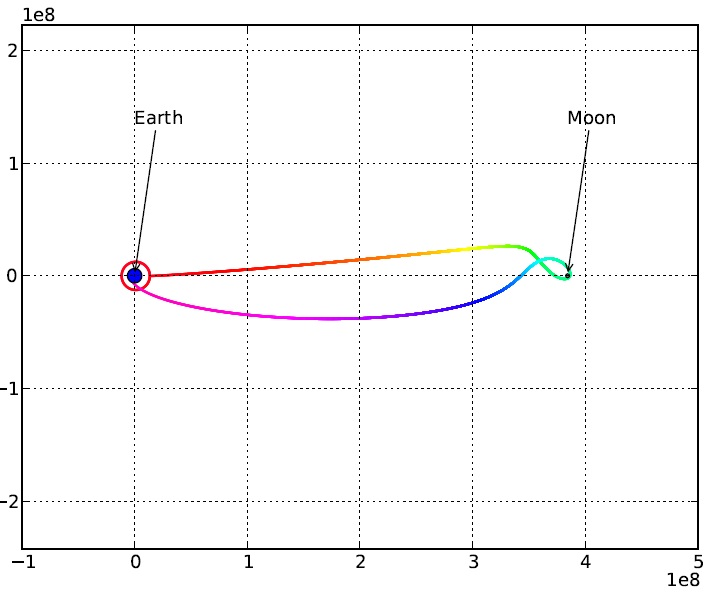
\includegraphics{moonshot.jpg}\hfill}


\chapter{Examples}
\label{examples::doc}\label{examples:examples}
For many people, it is easiest to learn a new library by adapting existing examples to
their purposes. For that reason, many examples are presented in this section in the
hope that they will prove useful to others using inspyred.


\section{Standard Algorithms}
\label{examples:standard-algorithms}
The following examples illustrate how to use the different, built-in, evolutionary computations.
They are (hopefully) simple and self-explanatory. Please note that each one uses an existing
benchmark problem. This is just an expedience; it is not necessary. The full list of existing
benchmarks can be found in the {\hyperref[reference::doc]{\emph{Library Reference}}}. See the {\hyperref[tutorial::doc]{\emph{Tutorial}}} for examples that
do not make use of a benchmark problem.


\subsection{Genetic Algorithm}
\label{examples:genetic-algorithm}
In this example, a GA is used to evolve a solution to the binary version of the Schwefel benchmark.
{[}\code{download}{]}

\begin{Verbatim}[commandchars=\\\{\}]
\PYG{k+kn}{from} \PYG{n+nn}{random} \PYG{k+kn}{import} \PYG{n}{Random}
\PYG{k+kn}{from} \PYG{n+nn}{time} \PYG{k+kn}{import} \PYG{n}{time}
\PYG{k+kn}{import} \PYG{n+nn}{inspyred}

\PYG{k}{def} \PYG{n+nf}{main}\PYG{p}{(}\PYG{n}{prng}\PYG{o}{=}\PYG{n+nb+bp}{None}\PYG{p}{,} \PYG{n}{display}\PYG{o}{=}\PYG{n+nb+bp}{False}\PYG{p}{)}\PYG{p}{:} 
    \PYG{k}{if} \PYG{n}{prng} \PYG{o+ow}{is} \PYG{n+nb+bp}{None}\PYG{p}{:}
        \PYG{n}{prng} \PYG{o}{=} \PYG{n}{Random}\PYG{p}{(}\PYG{p}{)}
        \PYG{n}{prng}\PYG{o}{.}\PYG{n}{seed}\PYG{p}{(}\PYG{n}{time}\PYG{p}{(}\PYG{p}{)}\PYG{p}{)} 
    
    \PYG{n}{problem} \PYG{o}{=} \PYG{n}{inspyred}\PYG{o}{.}\PYG{n}{benchmarks}\PYG{o}{.}\PYG{n}{Binary}\PYG{p}{(}\PYG{n}{inspyred}\PYG{o}{.}\PYG{n}{benchmarks}\PYG{o}{.}\PYG{n}{Schwefel}\PYG{p}{(}\PYG{l+m+mi}{2}\PYG{p}{)}\PYG{p}{,} 
                                         \PYG{n}{dimension\PYGZus{}bits}\PYG{o}{=}\PYG{l+m+mi}{30}\PYG{p}{)}
    \PYG{n}{ea} \PYG{o}{=} \PYG{n}{inspyred}\PYG{o}{.}\PYG{n}{ec}\PYG{o}{.}\PYG{n}{GA}\PYG{p}{(}\PYG{n}{prng}\PYG{p}{)}
    \PYG{n}{ea}\PYG{o}{.}\PYG{n}{terminator} \PYG{o}{=} \PYG{n}{inspyred}\PYG{o}{.}\PYG{n}{ec}\PYG{o}{.}\PYG{n}{terminators}\PYG{o}{.}\PYG{n}{evaluation\PYGZus{}termination}
    \PYG{n}{final\PYGZus{}pop} \PYG{o}{=} \PYG{n}{ea}\PYG{o}{.}\PYG{n}{evolve}\PYG{p}{(}\PYG{n}{generator}\PYG{o}{=}\PYG{n}{problem}\PYG{o}{.}\PYG{n}{generator}\PYG{p}{,}
                          \PYG{n}{evaluator}\PYG{o}{=}\PYG{n}{problem}\PYG{o}{.}\PYG{n}{evaluator}\PYG{p}{,}
                          \PYG{n}{pop\PYGZus{}size}\PYG{o}{=}\PYG{l+m+mi}{100}\PYG{p}{,}
                          \PYG{n}{maximize}\PYG{o}{=}\PYG{n}{problem}\PYG{o}{.}\PYG{n}{maximize}\PYG{p}{,}
                          \PYG{n}{bounder}\PYG{o}{=}\PYG{n}{problem}\PYG{o}{.}\PYG{n}{bounder}\PYG{p}{,}
                          \PYG{n}{max\PYGZus{}evaluations}\PYG{o}{=}\PYG{l+m+mi}{30000}\PYG{p}{,} 
                          \PYG{n}{num\PYGZus{}elites}\PYG{o}{=}\PYG{l+m+mi}{1}\PYG{p}{)}
                          
    \PYG{k}{if} \PYG{n}{display}\PYG{p}{:}
        \PYG{n}{best} \PYG{o}{=} \PYG{n+nb}{max}\PYG{p}{(}\PYG{n}{final\PYGZus{}pop}\PYG{p}{)}
        \PYG{k}{print}\PYG{p}{(}\PYG{l+s}{'}\PYG{l+s}{Best Solution: }\PYG{l+s+se}{\PYGZbs{}n}\PYG{l+s}{\PYGZob{}0\PYGZcb{}}\PYG{l+s}{'}\PYG{o}{.}\PYG{n}{format}\PYG{p}{(}\PYG{n+nb}{str}\PYG{p}{(}\PYG{n}{best}\PYG{p}{)}\PYG{p}{)}\PYG{p}{)}
    \PYG{k}{return} \PYG{n}{ea}
            
\PYG{k}{if} \PYG{n}{\PYGZus{}\PYGZus{}name\PYGZus{}\PYGZus{}} \PYG{o}{==} \PYG{l+s}{'}\PYG{l+s}{\PYGZus{}\PYGZus{}main\PYGZus{}\PYGZus{}}\PYG{l+s}{'}\PYG{p}{:}
    \PYG{n}{main}\PYG{p}{(}\PYG{n}{display}\PYG{o}{=}\PYG{n+nb+bp}{True}\PYG{p}{)}
\end{Verbatim}


\subsection{Evolution Strategy}
\label{examples:evolution-strategy}
In this example, an ES is used to evolve a solution to the Rosenbrock benchmark.
{[}\code{download}{]}

\begin{Verbatim}[commandchars=\\\{\}]
\PYG{k+kn}{from} \PYG{n+nn}{random} \PYG{k+kn}{import} \PYG{n}{Random}
\PYG{k+kn}{from} \PYG{n+nn}{time} \PYG{k+kn}{import} \PYG{n}{time}
\PYG{k+kn}{import} \PYG{n+nn}{inspyred}

\PYG{k}{def} \PYG{n+nf}{main}\PYG{p}{(}\PYG{n}{prng}\PYG{o}{=}\PYG{n+nb+bp}{None}\PYG{p}{,} \PYG{n}{display}\PYG{o}{=}\PYG{n+nb+bp}{False}\PYG{p}{)}\PYG{p}{:}    
    \PYG{k}{if} \PYG{n}{prng} \PYG{o+ow}{is} \PYG{n+nb+bp}{None}\PYG{p}{:}
        \PYG{n}{prng} \PYG{o}{=} \PYG{n}{Random}\PYG{p}{(}\PYG{p}{)}
        \PYG{n}{prng}\PYG{o}{.}\PYG{n}{seed}\PYG{p}{(}\PYG{n}{time}\PYG{p}{(}\PYG{p}{)}\PYG{p}{)} 
        
    \PYG{n}{problem} \PYG{o}{=} \PYG{n}{inspyred}\PYG{o}{.}\PYG{n}{benchmarks}\PYG{o}{.}\PYG{n}{Rosenbrock}\PYG{p}{(}\PYG{l+m+mi}{2}\PYG{p}{)}
    \PYG{n}{ea} \PYG{o}{=} \PYG{n}{inspyred}\PYG{o}{.}\PYG{n}{ec}\PYG{o}{.}\PYG{n}{ES}\PYG{p}{(}\PYG{n}{prng}\PYG{p}{)}
    \PYG{n}{ea}\PYG{o}{.}\PYG{n}{terminator} \PYG{o}{=} \PYG{p}{[}\PYG{n}{inspyred}\PYG{o}{.}\PYG{n}{ec}\PYG{o}{.}\PYG{n}{terminators}\PYG{o}{.}\PYG{n}{evaluation\PYGZus{}termination}\PYG{p}{,} 
                     \PYG{n}{inspyred}\PYG{o}{.}\PYG{n}{ec}\PYG{o}{.}\PYG{n}{terminators}\PYG{o}{.}\PYG{n}{diversity\PYGZus{}termination}\PYG{p}{]}
    \PYG{n}{final\PYGZus{}pop} \PYG{o}{=} \PYG{n}{ea}\PYG{o}{.}\PYG{n}{evolve}\PYG{p}{(}\PYG{n}{generator}\PYG{o}{=}\PYG{n}{problem}\PYG{o}{.}\PYG{n}{generator}\PYG{p}{,} 
                          \PYG{n}{evaluator}\PYG{o}{=}\PYG{n}{problem}\PYG{o}{.}\PYG{n}{evaluator}\PYG{p}{,} 
                          \PYG{n}{pop\PYGZus{}size}\PYG{o}{=}\PYG{l+m+mi}{100}\PYG{p}{,} 
                          \PYG{n}{bounder}\PYG{o}{=}\PYG{n}{problem}\PYG{o}{.}\PYG{n}{bounder}\PYG{p}{,}
                          \PYG{n}{maximize}\PYG{o}{=}\PYG{n}{problem}\PYG{o}{.}\PYG{n}{maximize}\PYG{p}{,}
                          \PYG{n}{max\PYGZus{}evaluations}\PYG{o}{=}\PYG{l+m+mi}{30000}\PYG{p}{)}

    \PYG{k}{if} \PYG{n}{display}\PYG{p}{:}
        \PYG{n}{best} \PYG{o}{=} \PYG{n+nb}{max}\PYG{p}{(}\PYG{n}{final\PYGZus{}pop}\PYG{p}{)}
        \PYG{k}{print}\PYG{p}{(}\PYG{l+s}{'}\PYG{l+s}{Best Solution: }\PYG{l+s+se}{\PYGZbs{}n}\PYG{l+s}{\PYGZob{}0\PYGZcb{}}\PYG{l+s}{'}\PYG{o}{.}\PYG{n}{format}\PYG{p}{(}\PYG{n+nb}{str}\PYG{p}{(}\PYG{n}{best}\PYG{p}{)}\PYG{p}{)}\PYG{p}{)}
    \PYG{k}{return} \PYG{n}{ea}
            
\PYG{k}{if} \PYG{n}{\PYGZus{}\PYGZus{}name\PYGZus{}\PYGZus{}} \PYG{o}{==} \PYG{l+s}{'}\PYG{l+s}{\PYGZus{}\PYGZus{}main\PYGZus{}\PYGZus{}}\PYG{l+s}{'}\PYG{p}{:}
    \PYG{n}{main}\PYG{p}{(}\PYG{n}{display}\PYG{o}{=}\PYG{n+nb+bp}{True}\PYG{p}{)}
\end{Verbatim}


\subsection{Simulated Annealing}
\label{examples:simulated-annealing}
In this example, an SA is used to evolve a solution to the Sphere benchmark.
{[}\code{download}{]}

\begin{Verbatim}[commandchars=\\\{\}]
\PYG{k+kn}{from} \PYG{n+nn}{random} \PYG{k+kn}{import} \PYG{n}{Random}
\PYG{k+kn}{from} \PYG{n+nn}{time} \PYG{k+kn}{import} \PYG{n}{time}
\PYG{k+kn}{import} \PYG{n+nn}{inspyred}

\PYG{k}{def} \PYG{n+nf}{main}\PYG{p}{(}\PYG{n}{prng}\PYG{o}{=}\PYG{n+nb+bp}{None}\PYG{p}{,} \PYG{n}{display}\PYG{o}{=}\PYG{n+nb+bp}{False}\PYG{p}{)}\PYG{p}{:}    
    \PYG{k}{if} \PYG{n}{prng} \PYG{o+ow}{is} \PYG{n+nb+bp}{None}\PYG{p}{:}
        \PYG{n}{prng} \PYG{o}{=} \PYG{n}{Random}\PYG{p}{(}\PYG{p}{)}
        \PYG{n}{prng}\PYG{o}{.}\PYG{n}{seed}\PYG{p}{(}\PYG{n}{time}\PYG{p}{(}\PYG{p}{)}\PYG{p}{)} 
        
    \PYG{n}{problem} \PYG{o}{=} \PYG{n}{inspyred}\PYG{o}{.}\PYG{n}{benchmarks}\PYG{o}{.}\PYG{n}{Sphere}\PYG{p}{(}\PYG{l+m+mi}{2}\PYG{p}{)}
    \PYG{n}{ea} \PYG{o}{=} \PYG{n}{inspyred}\PYG{o}{.}\PYG{n}{ec}\PYG{o}{.}\PYG{n}{SA}\PYG{p}{(}\PYG{n}{prng}\PYG{p}{)}
    \PYG{n}{ea}\PYG{o}{.}\PYG{n}{terminator} \PYG{o}{=} \PYG{n}{inspyred}\PYG{o}{.}\PYG{n}{ec}\PYG{o}{.}\PYG{n}{terminators}\PYG{o}{.}\PYG{n}{evaluation\PYGZus{}termination}
    \PYG{n}{final\PYGZus{}pop} \PYG{o}{=} \PYG{n}{ea}\PYG{o}{.}\PYG{n}{evolve}\PYG{p}{(}\PYG{n}{evaluator}\PYG{o}{=}\PYG{n}{problem}\PYG{o}{.}\PYG{n}{evaluator}\PYG{p}{,} 
                          \PYG{n}{generator}\PYG{o}{=}\PYG{n}{problem}\PYG{o}{.}\PYG{n}{generator}\PYG{p}{,} 
                          \PYG{n}{maximize}\PYG{o}{=}\PYG{n}{problem}\PYG{o}{.}\PYG{n}{maximize}\PYG{p}{,}
                          \PYG{n}{bounder}\PYG{o}{=}\PYG{n}{problem}\PYG{o}{.}\PYG{n}{bounder}\PYG{p}{,}
                          \PYG{n}{max\PYGZus{}evaluations}\PYG{o}{=}\PYG{l+m+mi}{30000}\PYG{p}{)}
                          
    \PYG{k}{if} \PYG{n}{display}\PYG{p}{:}
        \PYG{n}{best} \PYG{o}{=} \PYG{n+nb}{max}\PYG{p}{(}\PYG{n}{final\PYGZus{}pop}\PYG{p}{)}
        \PYG{k}{print}\PYG{p}{(}\PYG{l+s}{'}\PYG{l+s}{Best Solution: }\PYG{l+s+se}{\PYGZbs{}n}\PYG{l+s}{\PYGZob{}0\PYGZcb{}}\PYG{l+s}{'}\PYG{o}{.}\PYG{n}{format}\PYG{p}{(}\PYG{n+nb}{str}\PYG{p}{(}\PYG{n}{best}\PYG{p}{)}\PYG{p}{)}\PYG{p}{)}
    \PYG{k}{return} \PYG{n}{ea}
            
\PYG{k}{if} \PYG{n}{\PYGZus{}\PYGZus{}name\PYGZus{}\PYGZus{}} \PYG{o}{==} \PYG{l+s}{'}\PYG{l+s}{\PYGZus{}\PYGZus{}main\PYGZus{}\PYGZus{}}\PYG{l+s}{'}\PYG{p}{:}
    \PYG{n}{main}\PYG{p}{(}\PYG{n}{display}\PYG{o}{=}\PYG{n+nb+bp}{True}\PYG{p}{)}
\end{Verbatim}


\subsection{Differential Evolution Algorithm}
\label{examples:differential-evolution-algorithm}
In this example, a DEA is used to evolve a solution to the Griewank benchmark.
{[}\code{download}{]}

\begin{Verbatim}[commandchars=\\\{\}]
\PYG{k+kn}{from} \PYG{n+nn}{random} \PYG{k+kn}{import} \PYG{n}{Random}
\PYG{k+kn}{from} \PYG{n+nn}{time} \PYG{k+kn}{import} \PYG{n}{time}
\PYG{k+kn}{import} \PYG{n+nn}{inspyred}

\PYG{k}{def} \PYG{n+nf}{main}\PYG{p}{(}\PYG{n}{prng}\PYG{o}{=}\PYG{n+nb+bp}{None}\PYG{p}{,} \PYG{n}{display}\PYG{o}{=}\PYG{n+nb+bp}{False}\PYG{p}{)}\PYG{p}{:}
    \PYG{k}{if} \PYG{n}{prng} \PYG{o+ow}{is} \PYG{n+nb+bp}{None}\PYG{p}{:}
        \PYG{n}{prng} \PYG{o}{=} \PYG{n}{Random}\PYG{p}{(}\PYG{p}{)}
        \PYG{n}{prng}\PYG{o}{.}\PYG{n}{seed}\PYG{p}{(}\PYG{n}{time}\PYG{p}{(}\PYG{p}{)}\PYG{p}{)} 
    
    \PYG{n}{problem} \PYG{o}{=} \PYG{n}{inspyred}\PYG{o}{.}\PYG{n}{benchmarks}\PYG{o}{.}\PYG{n}{Griewank}\PYG{p}{(}\PYG{l+m+mi}{2}\PYG{p}{)}
    \PYG{n}{ea} \PYG{o}{=} \PYG{n}{inspyred}\PYG{o}{.}\PYG{n}{ec}\PYG{o}{.}\PYG{n}{DEA}\PYG{p}{(}\PYG{n}{prng}\PYG{p}{)}
    \PYG{n}{ea}\PYG{o}{.}\PYG{n}{terminator} \PYG{o}{=} \PYG{n}{inspyred}\PYG{o}{.}\PYG{n}{ec}\PYG{o}{.}\PYG{n}{terminators}\PYG{o}{.}\PYG{n}{evaluation\PYGZus{}termination}
    \PYG{n}{final\PYGZus{}pop} \PYG{o}{=} \PYG{n}{ea}\PYG{o}{.}\PYG{n}{evolve}\PYG{p}{(}\PYG{n}{generator}\PYG{o}{=}\PYG{n}{problem}\PYG{o}{.}\PYG{n}{generator}\PYG{p}{,} 
                          \PYG{n}{evaluator}\PYG{o}{=}\PYG{n}{problem}\PYG{o}{.}\PYG{n}{evaluator}\PYG{p}{,} 
                          \PYG{n}{pop\PYGZus{}size}\PYG{o}{=}\PYG{l+m+mi}{100}\PYG{p}{,} 
                          \PYG{n}{bounder}\PYG{o}{=}\PYG{n}{problem}\PYG{o}{.}\PYG{n}{bounder}\PYG{p}{,}
                          \PYG{n}{maximize}\PYG{o}{=}\PYG{n}{problem}\PYG{o}{.}\PYG{n}{maximize}\PYG{p}{,}
                          \PYG{n}{max\PYGZus{}evaluations}\PYG{o}{=}\PYG{l+m+mi}{30000}\PYG{p}{)}
                          
    \PYG{k}{if} \PYG{n}{display}\PYG{p}{:}
        \PYG{n}{best} \PYG{o}{=} \PYG{n+nb}{max}\PYG{p}{(}\PYG{n}{final\PYGZus{}pop}\PYG{p}{)}
        \PYG{k}{print}\PYG{p}{(}\PYG{l+s}{'}\PYG{l+s}{Best Solution: }\PYG{l+s+se}{\PYGZbs{}n}\PYG{l+s}{\PYGZob{}0\PYGZcb{}}\PYG{l+s}{'}\PYG{o}{.}\PYG{n}{format}\PYG{p}{(}\PYG{n+nb}{str}\PYG{p}{(}\PYG{n}{best}\PYG{p}{)}\PYG{p}{)}\PYG{p}{)}
    \PYG{k}{return} \PYG{n}{ea}

\PYG{k}{if} \PYG{n}{\PYGZus{}\PYGZus{}name\PYGZus{}\PYGZus{}} \PYG{o}{==} \PYG{l+s}{'}\PYG{l+s}{\PYGZus{}\PYGZus{}main\PYGZus{}\PYGZus{}}\PYG{l+s}{'}\PYG{p}{:}
    \PYG{n}{main}\PYG{p}{(}\PYG{n}{display}\PYG{o}{=}\PYG{n+nb+bp}{True}\PYG{p}{)}
\end{Verbatim}


\subsection{Estimation of Distribution Algorithm}
\label{examples:estimation-of-distribution-algorithm}
In this example, an EDA is used to evolve a solution to the Rastrigin benchmark.
{[}\code{download}{]}

\begin{Verbatim}[commandchars=\\\{\}]
\PYG{k+kn}{from} \PYG{n+nn}{random} \PYG{k+kn}{import} \PYG{n}{Random}
\PYG{k+kn}{from} \PYG{n+nn}{time} \PYG{k+kn}{import} \PYG{n}{time}
\PYG{k+kn}{import} \PYG{n+nn}{inspyred}

\PYG{k}{def} \PYG{n+nf}{main}\PYG{p}{(}\PYG{n}{prng}\PYG{o}{=}\PYG{n+nb+bp}{None}\PYG{p}{,} \PYG{n}{display}\PYG{o}{=}\PYG{n+nb+bp}{False}\PYG{p}{)}\PYG{p}{:}
    \PYG{k}{if} \PYG{n}{prng} \PYG{o+ow}{is} \PYG{n+nb+bp}{None}\PYG{p}{:}
        \PYG{n}{prng} \PYG{o}{=} \PYG{n}{Random}\PYG{p}{(}\PYG{p}{)}
        \PYG{n}{prng}\PYG{o}{.}\PYG{n}{seed}\PYG{p}{(}\PYG{n}{time}\PYG{p}{(}\PYG{p}{)}\PYG{p}{)} 
    
    \PYG{n}{problem} \PYG{o}{=} \PYG{n}{inspyred}\PYG{o}{.}\PYG{n}{benchmarks}\PYG{o}{.}\PYG{n}{Rastrigin}\PYG{p}{(}\PYG{l+m+mi}{2}\PYG{p}{)}
    \PYG{n}{ea} \PYG{o}{=} \PYG{n}{inspyred}\PYG{o}{.}\PYG{n}{ec}\PYG{o}{.}\PYG{n}{EDA}\PYG{p}{(}\PYG{n}{prng}\PYG{p}{)}
    \PYG{n}{ea}\PYG{o}{.}\PYG{n}{terminator} \PYG{o}{=} \PYG{n}{inspyred}\PYG{o}{.}\PYG{n}{ec}\PYG{o}{.}\PYG{n}{terminators}\PYG{o}{.}\PYG{n}{evaluation\PYGZus{}termination}
    \PYG{n}{final\PYGZus{}pop} \PYG{o}{=} \PYG{n}{ea}\PYG{o}{.}\PYG{n}{evolve}\PYG{p}{(}\PYG{n}{evaluator}\PYG{o}{=}\PYG{n}{problem}\PYG{o}{.}\PYG{n}{evaluator}\PYG{p}{,} 
                          \PYG{n}{generator}\PYG{o}{=}\PYG{n}{problem}\PYG{o}{.}\PYG{n}{generator}\PYG{p}{,} 
                          \PYG{n}{pop\PYGZus{}size}\PYG{o}{=}\PYG{l+m+mi}{1000}\PYG{p}{,} 
                          \PYG{n}{bounder}\PYG{o}{=}\PYG{n}{problem}\PYG{o}{.}\PYG{n}{bounder}\PYG{p}{,}
                          \PYG{n}{maximize}\PYG{o}{=}\PYG{n}{problem}\PYG{o}{.}\PYG{n}{maximize}\PYG{p}{,}
                          \PYG{n}{max\PYGZus{}evaluations}\PYG{o}{=}\PYG{l+m+mi}{30000}\PYG{p}{,}
                          \PYG{n}{num\PYGZus{}selected}\PYG{o}{=}\PYG{l+m+mi}{500}\PYG{p}{,}
                          \PYG{n}{num\PYGZus{}offspring}\PYG{o}{=}\PYG{l+m+mi}{1000}\PYG{p}{,}
                          \PYG{n}{num\PYGZus{}elites}\PYG{o}{=}\PYG{l+m+mi}{1}\PYG{p}{)}
    
    \PYG{k}{if} \PYG{n}{display}\PYG{p}{:}
        \PYG{n}{best} \PYG{o}{=} \PYG{n+nb}{max}\PYG{p}{(}\PYG{n}{final\PYGZus{}pop}\PYG{p}{)} 
        \PYG{k}{print}\PYG{p}{(}\PYG{l+s}{'}\PYG{l+s}{Best Solution: }\PYG{l+s+se}{\PYGZbs{}n}\PYG{l+s}{\PYGZob{}0\PYGZcb{}}\PYG{l+s}{'}\PYG{o}{.}\PYG{n}{format}\PYG{p}{(}\PYG{n+nb}{str}\PYG{p}{(}\PYG{n}{best}\PYG{p}{)}\PYG{p}{)}\PYG{p}{)}
    \PYG{k}{return} \PYG{n}{ea}
            
\PYG{k}{if} \PYG{n}{\PYGZus{}\PYGZus{}name\PYGZus{}\PYGZus{}} \PYG{o}{==} \PYG{l+s}{'}\PYG{l+s}{\PYGZus{}\PYGZus{}main\PYGZus{}\PYGZus{}}\PYG{l+s}{'}\PYG{p}{:}
    \PYG{n}{main}\PYG{p}{(}\PYG{n}{display}\PYG{o}{=}\PYG{n+nb+bp}{True}\PYG{p}{)}
\end{Verbatim}


\subsection{Pareto Archived Evolution Strategy (PAES)}
\label{examples:pareto-archived-evolution-strategy-paes}
In this example, a PAES is used to evolve a solution to the Kursawe multiobjective benchmark.
{[}\code{download}{]}

\begin{Verbatim}[commandchars=\\\{\}]
\PYG{k+kn}{from} \PYG{n+nn}{random} \PYG{k+kn}{import} \PYG{n}{Random}
\PYG{k+kn}{from} \PYG{n+nn}{time} \PYG{k+kn}{import} \PYG{n}{time}
\PYG{k+kn}{import} \PYG{n+nn}{inspyred}

\PYG{k}{def} \PYG{n+nf}{main}\PYG{p}{(}\PYG{n}{prng}\PYG{o}{=}\PYG{n+nb+bp}{None}\PYG{p}{,} \PYG{n}{display}\PYG{o}{=}\PYG{n+nb+bp}{False}\PYG{p}{)}\PYG{p}{:}
    \PYG{k}{if} \PYG{n}{prng} \PYG{o+ow}{is} \PYG{n+nb+bp}{None}\PYG{p}{:}
        \PYG{n}{prng} \PYG{o}{=} \PYG{n}{Random}\PYG{p}{(}\PYG{p}{)}
        \PYG{n}{prng}\PYG{o}{.}\PYG{n}{seed}\PYG{p}{(}\PYG{n}{time}\PYG{p}{(}\PYG{p}{)}\PYG{p}{)} 
        
    \PYG{n}{problem} \PYG{o}{=} \PYG{n}{inspyred}\PYG{o}{.}\PYG{n}{benchmarks}\PYG{o}{.}\PYG{n}{Kursawe}\PYG{p}{(}\PYG{l+m+mi}{3}\PYG{p}{)}
    \PYG{n}{ea} \PYG{o}{=} \PYG{n}{inspyred}\PYG{o}{.}\PYG{n}{ec}\PYG{o}{.}\PYG{n}{emo}\PYG{o}{.}\PYG{n}{PAES}\PYG{p}{(}\PYG{n}{prng}\PYG{p}{)}
    \PYG{n}{ea}\PYG{o}{.}\PYG{n}{terminator} \PYG{o}{=} \PYG{n}{inspyred}\PYG{o}{.}\PYG{n}{ec}\PYG{o}{.}\PYG{n}{terminators}\PYG{o}{.}\PYG{n}{evaluation\PYGZus{}termination}
    \PYG{n}{final\PYGZus{}pop} \PYG{o}{=} \PYG{n}{ea}\PYG{o}{.}\PYG{n}{evolve}\PYG{p}{(}\PYG{n}{generator}\PYG{o}{=}\PYG{n}{problem}\PYG{o}{.}\PYG{n}{generator}\PYG{p}{,} 
                          \PYG{n}{evaluator}\PYG{o}{=}\PYG{n}{problem}\PYG{o}{.}\PYG{n}{evaluator}\PYG{p}{,} 
                          \PYG{n}{bounder}\PYG{o}{=}\PYG{n}{problem}\PYG{o}{.}\PYG{n}{bounder}\PYG{p}{,}
                          \PYG{n}{maximize}\PYG{o}{=}\PYG{n}{problem}\PYG{o}{.}\PYG{n}{maximize}\PYG{p}{,}
                          \PYG{n}{max\PYGZus{}evaluations}\PYG{o}{=}\PYG{l+m+mi}{10000}\PYG{p}{,}
                          \PYG{n}{max\PYGZus{}archive\PYGZus{}size}\PYG{o}{=}\PYG{l+m+mi}{100}\PYG{p}{,}
                          \PYG{n}{num\PYGZus{}grid\PYGZus{}divisions}\PYG{o}{=}\PYG{l+m+mi}{4}\PYG{p}{)}
    
    \PYG{k}{if} \PYG{n}{display}\PYG{p}{:}
        \PYG{n}{final\PYGZus{}arc} \PYG{o}{=} \PYG{n}{ea}\PYG{o}{.}\PYG{n}{archive}
        \PYG{k}{print}\PYG{p}{(}\PYG{l+s}{'}\PYG{l+s}{Best Solutions: }\PYG{l+s+se}{\PYGZbs{}n}\PYG{l+s}{'}\PYG{p}{)}
        \PYG{k}{for} \PYG{n}{f} \PYG{o+ow}{in} \PYG{n}{final\PYGZus{}arc}\PYG{p}{:}
            \PYG{k}{print}\PYG{p}{(}\PYG{n}{f}\PYG{p}{)}
        \PYG{k+kn}{import} \PYG{n+nn}{pylab}
        \PYG{n}{x} \PYG{o}{=} \PYG{p}{[}\PYG{p}{]}
        \PYG{n}{y} \PYG{o}{=} \PYG{p}{[}\PYG{p}{]}
        \PYG{k}{for} \PYG{n}{f} \PYG{o+ow}{in} \PYG{n}{final\PYGZus{}arc}\PYG{p}{:}
            \PYG{n}{x}\PYG{o}{.}\PYG{n}{append}\PYG{p}{(}\PYG{n}{f}\PYG{o}{.}\PYG{n}{fitness}\PYG{p}{[}\PYG{l+m+mi}{0}\PYG{p}{]}\PYG{p}{)}
            \PYG{n}{y}\PYG{o}{.}\PYG{n}{append}\PYG{p}{(}\PYG{n}{f}\PYG{o}{.}\PYG{n}{fitness}\PYG{p}{[}\PYG{l+m+mi}{1}\PYG{p}{]}\PYG{p}{)}
        \PYG{n}{pylab}\PYG{o}{.}\PYG{n}{scatter}\PYG{p}{(}\PYG{n}{x}\PYG{p}{,} \PYG{n}{y}\PYG{p}{,} \PYG{n}{color}\PYG{o}{=}\PYG{l+s}{'}\PYG{l+s}{b}\PYG{l+s}{'}\PYG{p}{)}
        \PYG{n}{pylab}\PYG{o}{.}\PYG{n}{savefig}\PYG{p}{(}\PYG{l+s}{'}\PYG{l+s}{\PYGZob{}0\PYGZcb{} Example (\PYGZob{}1\PYGZcb{}).pdf}\PYG{l+s}{'}\PYG{o}{.}\PYG{n}{format}\PYG{p}{(}\PYG{n}{ea}\PYG{o}{.}\PYG{n}{\PYGZus{}\PYGZus{}class\PYGZus{}\PYGZus{}}\PYG{o}{.}\PYG{n}{\PYGZus{}\PYGZus{}name\PYGZus{}\PYGZus{}}\PYG{p}{,} 
                                                     \PYG{n}{problem}\PYG{o}{.}\PYG{n}{\PYGZus{}\PYGZus{}class\PYGZus{}\PYGZus{}}\PYG{o}{.}\PYG{n}{\PYGZus{}\PYGZus{}name\PYGZus{}\PYGZus{}}\PYG{p}{)}\PYG{p}{,} 
                      \PYG{n}{format}\PYG{o}{=}\PYG{l+s}{'}\PYG{l+s}{pdf}\PYG{l+s}{'}\PYG{p}{)}
        \PYG{n}{pylab}\PYG{o}{.}\PYG{n}{show}\PYG{p}{(}\PYG{p}{)}
    \PYG{k}{return} \PYG{n}{ea}

\PYG{k}{if} \PYG{n}{\PYGZus{}\PYGZus{}name\PYGZus{}\PYGZus{}} \PYG{o}{==} \PYG{l+s}{'}\PYG{l+s}{\PYGZus{}\PYGZus{}main\PYGZus{}\PYGZus{}}\PYG{l+s}{'}\PYG{p}{:}
    \PYG{n}{main}\PYG{p}{(}\PYG{n}{display}\PYG{o}{=}\PYG{n+nb+bp}{True}\PYG{p}{)}
\end{Verbatim}


\subsection{Nondominated Sorting Genetic Algorithm (NSGA-II)}
\label{examples:nondominated-sorting-genetic-algorithm-nsga-ii}
In this example, an NSGA2 is used to evolve a solution to the Kursawe multiobjective benchmark.
{[}\code{download}{]}

\begin{Verbatim}[commandchars=\\\{\}]
\PYG{k+kn}{from} \PYG{n+nn}{random} \PYG{k+kn}{import} \PYG{n}{Random}
\PYG{k+kn}{from} \PYG{n+nn}{time} \PYG{k+kn}{import} \PYG{n}{time}
\PYG{k+kn}{import} \PYG{n+nn}{inspyred}
   
\PYG{k}{def} \PYG{n+nf}{main}\PYG{p}{(}\PYG{n}{prng}\PYG{o}{=}\PYG{n+nb+bp}{None}\PYG{p}{,} \PYG{n}{display}\PYG{o}{=}\PYG{n+nb+bp}{False}\PYG{p}{)}\PYG{p}{:}
    \PYG{k}{if} \PYG{n}{prng} \PYG{o+ow}{is} \PYG{n+nb+bp}{None}\PYG{p}{:}
        \PYG{n}{prng} \PYG{o}{=} \PYG{n}{Random}\PYG{p}{(}\PYG{p}{)}
        \PYG{n}{prng}\PYG{o}{.}\PYG{n}{seed}\PYG{p}{(}\PYG{n}{time}\PYG{p}{(}\PYG{p}{)}\PYG{p}{)} 

    \PYG{n}{problem} \PYG{o}{=} \PYG{n}{inspyred}\PYG{o}{.}\PYG{n}{benchmarks}\PYG{o}{.}\PYG{n}{Kursawe}\PYG{p}{(}\PYG{l+m+mi}{3}\PYG{p}{)}
    \PYG{n}{ea} \PYG{o}{=} \PYG{n}{inspyred}\PYG{o}{.}\PYG{n}{ec}\PYG{o}{.}\PYG{n}{emo}\PYG{o}{.}\PYG{n}{NSGA2}\PYG{p}{(}\PYG{n}{prng}\PYG{p}{)}
    \PYG{n}{ea}\PYG{o}{.}\PYG{n}{variator} \PYG{o}{=} \PYG{p}{[}\PYG{n}{inspyred}\PYG{o}{.}\PYG{n}{ec}\PYG{o}{.}\PYG{n}{variators}\PYG{o}{.}\PYG{n}{blend\PYGZus{}crossover}\PYG{p}{,} 
                   \PYG{n}{inspyred}\PYG{o}{.}\PYG{n}{ec}\PYG{o}{.}\PYG{n}{variators}\PYG{o}{.}\PYG{n}{gaussian\PYGZus{}mutation}\PYG{p}{]}
    \PYG{n}{ea}\PYG{o}{.}\PYG{n}{terminator} \PYG{o}{=} \PYG{n}{inspyred}\PYG{o}{.}\PYG{n}{ec}\PYG{o}{.}\PYG{n}{terminators}\PYG{o}{.}\PYG{n}{generation\PYGZus{}termination}
    \PYG{n}{final\PYGZus{}pop} \PYG{o}{=} \PYG{n}{ea}\PYG{o}{.}\PYG{n}{evolve}\PYG{p}{(}\PYG{n}{generator}\PYG{o}{=}\PYG{n}{problem}\PYG{o}{.}\PYG{n}{generator}\PYG{p}{,} 
                          \PYG{n}{evaluator}\PYG{o}{=}\PYG{n}{problem}\PYG{o}{.}\PYG{n}{evaluator}\PYG{p}{,} 
                          \PYG{n}{pop\PYGZus{}size}\PYG{o}{=}\PYG{l+m+mi}{100}\PYG{p}{,}
                          \PYG{n}{maximize}\PYG{o}{=}\PYG{n}{problem}\PYG{o}{.}\PYG{n}{maximize}\PYG{p}{,}
                          \PYG{n}{bounder}\PYG{o}{=}\PYG{n}{problem}\PYG{o}{.}\PYG{n}{bounder}\PYG{p}{,}
                          \PYG{n}{max\PYGZus{}generations}\PYG{o}{=}\PYG{l+m+mi}{80}\PYG{p}{)}
    
    \PYG{k}{if} \PYG{n}{display}\PYG{p}{:}
        \PYG{n}{final\PYGZus{}arc} \PYG{o}{=} \PYG{n}{ea}\PYG{o}{.}\PYG{n}{archive}
        \PYG{k}{print}\PYG{p}{(}\PYG{l+s}{'}\PYG{l+s}{Best Solutions: }\PYG{l+s+se}{\PYGZbs{}n}\PYG{l+s}{'}\PYG{p}{)}
        \PYG{k}{for} \PYG{n}{f} \PYG{o+ow}{in} \PYG{n}{final\PYGZus{}arc}\PYG{p}{:}
            \PYG{k}{print}\PYG{p}{(}\PYG{n}{f}\PYG{p}{)}
        \PYG{k+kn}{import} \PYG{n+nn}{pylab}
        \PYG{n}{x} \PYG{o}{=} \PYG{p}{[}\PYG{p}{]}
        \PYG{n}{y} \PYG{o}{=} \PYG{p}{[}\PYG{p}{]}
        \PYG{k}{for} \PYG{n}{f} \PYG{o+ow}{in} \PYG{n}{final\PYGZus{}arc}\PYG{p}{:}
            \PYG{n}{x}\PYG{o}{.}\PYG{n}{append}\PYG{p}{(}\PYG{n}{f}\PYG{o}{.}\PYG{n}{fitness}\PYG{p}{[}\PYG{l+m+mi}{0}\PYG{p}{]}\PYG{p}{)}
            \PYG{n}{y}\PYG{o}{.}\PYG{n}{append}\PYG{p}{(}\PYG{n}{f}\PYG{o}{.}\PYG{n}{fitness}\PYG{p}{[}\PYG{l+m+mi}{1}\PYG{p}{]}\PYG{p}{)}
        \PYG{n}{pylab}\PYG{o}{.}\PYG{n}{scatter}\PYG{p}{(}\PYG{n}{x}\PYG{p}{,} \PYG{n}{y}\PYG{p}{,} \PYG{n}{color}\PYG{o}{=}\PYG{l+s}{'}\PYG{l+s}{b}\PYG{l+s}{'}\PYG{p}{)}
        \PYG{n}{pylab}\PYG{o}{.}\PYG{n}{savefig}\PYG{p}{(}\PYG{l+s}{'}\PYG{l+s}{\PYGZob{}0\PYGZcb{} Example (\PYGZob{}1\PYGZcb{}).pdf}\PYG{l+s}{'}\PYG{o}{.}\PYG{n}{format}\PYG{p}{(}\PYG{n}{ea}\PYG{o}{.}\PYG{n}{\PYGZus{}\PYGZus{}class\PYGZus{}\PYGZus{}}\PYG{o}{.}\PYG{n}{\PYGZus{}\PYGZus{}name\PYGZus{}\PYGZus{}}\PYG{p}{,} 
                                                     \PYG{n}{problem}\PYG{o}{.}\PYG{n}{\PYGZus{}\PYGZus{}class\PYGZus{}\PYGZus{}}\PYG{o}{.}\PYG{n}{\PYGZus{}\PYGZus{}name\PYGZus{}\PYGZus{}}\PYG{p}{)}\PYG{p}{,} 
                      \PYG{n}{format}\PYG{o}{=}\PYG{l+s}{'}\PYG{l+s}{pdf}\PYG{l+s}{'}\PYG{p}{)}
        \PYG{n}{pylab}\PYG{o}{.}\PYG{n}{show}\PYG{p}{(}\PYG{p}{)}
    \PYG{k}{return} \PYG{n}{ea}
        
\PYG{k}{if} \PYG{n}{\PYGZus{}\PYGZus{}name\PYGZus{}\PYGZus{}} \PYG{o}{==} \PYG{l+s}{'}\PYG{l+s}{\PYGZus{}\PYGZus{}main\PYGZus{}\PYGZus{}}\PYG{l+s}{'}\PYG{p}{:}
    \PYG{n}{main}\PYG{p}{(}\PYG{n}{display}\PYG{o}{=}\PYG{n+nb+bp}{True}\PYG{p}{)}
\end{Verbatim}


\subsection{Particle Swarm Optimization}
\label{examples:particle-swarm-optimization}
In this example, a PSO is used to evolve a solution to the Ackley benchmark.
{[}\code{download}{]}

\begin{Verbatim}[commandchars=\\\{\}]
\PYG{k+kn}{from} \PYG{n+nn}{time} \PYG{k+kn}{import} \PYG{n}{time}
\PYG{k+kn}{from} \PYG{n+nn}{random} \PYG{k+kn}{import} \PYG{n}{Random}
\PYG{k+kn}{import} \PYG{n+nn}{inspyred}

\PYG{k}{def} \PYG{n+nf}{main}\PYG{p}{(}\PYG{n}{prng}\PYG{o}{=}\PYG{n+nb+bp}{None}\PYG{p}{,} \PYG{n}{display}\PYG{o}{=}\PYG{n+nb+bp}{False}\PYG{p}{)}\PYG{p}{:}
    \PYG{k}{if} \PYG{n}{prng} \PYG{o+ow}{is} \PYG{n+nb+bp}{None}\PYG{p}{:}
        \PYG{n}{prng} \PYG{o}{=} \PYG{n}{Random}\PYG{p}{(}\PYG{p}{)}
        \PYG{n}{prng}\PYG{o}{.}\PYG{n}{seed}\PYG{p}{(}\PYG{n}{time}\PYG{p}{(}\PYG{p}{)}\PYG{p}{)} 
    
    \PYG{n}{problem} \PYG{o}{=} \PYG{n}{inspyred}\PYG{o}{.}\PYG{n}{benchmarks}\PYG{o}{.}\PYG{n}{Ackley}\PYG{p}{(}\PYG{l+m+mi}{2}\PYG{p}{)}
    \PYG{n}{ea} \PYG{o}{=} \PYG{n}{inspyred}\PYG{o}{.}\PYG{n}{swarm}\PYG{o}{.}\PYG{n}{PSO}\PYG{p}{(}\PYG{n}{prng}\PYG{p}{)}
    \PYG{n}{ea}\PYG{o}{.}\PYG{n}{terminator} \PYG{o}{=} \PYG{n}{inspyred}\PYG{o}{.}\PYG{n}{ec}\PYG{o}{.}\PYG{n}{terminators}\PYG{o}{.}\PYG{n}{evaluation\PYGZus{}termination}
    \PYG{n}{ea}\PYG{o}{.}\PYG{n}{topology} \PYG{o}{=} \PYG{n}{inspyred}\PYG{o}{.}\PYG{n}{swarm}\PYG{o}{.}\PYG{n}{topologies}\PYG{o}{.}\PYG{n}{ring\PYGZus{}topology}
    \PYG{n}{final\PYGZus{}pop} \PYG{o}{=} \PYG{n}{ea}\PYG{o}{.}\PYG{n}{evolve}\PYG{p}{(}\PYG{n}{generator}\PYG{o}{=}\PYG{n}{problem}\PYG{o}{.}\PYG{n}{generator}\PYG{p}{,}
                          \PYG{n}{evaluator}\PYG{o}{=}\PYG{n}{problem}\PYG{o}{.}\PYG{n}{evaluator}\PYG{p}{,} 
                          \PYG{n}{pop\PYGZus{}size}\PYG{o}{=}\PYG{l+m+mi}{100}\PYG{p}{,}
                          \PYG{n}{bounder}\PYG{o}{=}\PYG{n}{problem}\PYG{o}{.}\PYG{n}{bounder}\PYG{p}{,}
                          \PYG{n}{maximize}\PYG{o}{=}\PYG{n}{problem}\PYG{o}{.}\PYG{n}{maximize}\PYG{p}{,}
                          \PYG{n}{max\PYGZus{}evaluations}\PYG{o}{=}\PYG{l+m+mi}{30000}\PYG{p}{,} 
                          \PYG{n}{neighborhood\PYGZus{}size}\PYG{o}{=}\PYG{l+m+mi}{5}\PYG{p}{)}

    \PYG{k}{if} \PYG{n}{display}\PYG{p}{:}
        \PYG{n}{best} \PYG{o}{=} \PYG{n+nb}{max}\PYG{p}{(}\PYG{n}{final\PYGZus{}pop}\PYG{p}{)} 
        \PYG{k}{print}\PYG{p}{(}\PYG{l+s}{'}\PYG{l+s}{Best Solution: }\PYG{l+s+se}{\PYGZbs{}n}\PYG{l+s}{\PYGZob{}0\PYGZcb{}}\PYG{l+s}{'}\PYG{o}{.}\PYG{n}{format}\PYG{p}{(}\PYG{n+nb}{str}\PYG{p}{(}\PYG{n}{best}\PYG{p}{)}\PYG{p}{)}\PYG{p}{)}
    \PYG{k}{return} \PYG{n}{ea}

\PYG{k}{if} \PYG{n}{\PYGZus{}\PYGZus{}name\PYGZus{}\PYGZus{}} \PYG{o}{==} \PYG{l+s}{'}\PYG{l+s}{\PYGZus{}\PYGZus{}main\PYGZus{}\PYGZus{}}\PYG{l+s}{'}\PYG{p}{:}
    \PYG{n}{main}\PYG{p}{(}\PYG{n}{display}\PYG{o}{=}\PYG{n+nb+bp}{True}\PYG{p}{)}
\end{Verbatim}


\subsection{Ant Colony Optimization}
\label{examples:ant-colony-optimization}
In this example, an ACS is used to evolve a solution to the TSP benchmark.
{[}\code{download}{]}

\begin{Verbatim}[commandchars=\\\{\}]
\PYG{k+kn}{from} \PYG{n+nn}{random} \PYG{k+kn}{import} \PYG{n}{Random}
\PYG{k+kn}{from} \PYG{n+nn}{time} \PYG{k+kn}{import} \PYG{n}{time}
\PYG{k+kn}{import} \PYG{n+nn}{math}
\PYG{k+kn}{import} \PYG{n+nn}{inspyred}

\PYG{k}{def} \PYG{n+nf}{main}\PYG{p}{(}\PYG{n}{prng}\PYG{o}{=}\PYG{n+nb+bp}{None}\PYG{p}{,} \PYG{n}{display}\PYG{o}{=}\PYG{n+nb+bp}{False}\PYG{p}{)}\PYG{p}{:}    
    \PYG{k}{if} \PYG{n}{prng} \PYG{o+ow}{is} \PYG{n+nb+bp}{None}\PYG{p}{:}
        \PYG{n}{prng} \PYG{o}{=} \PYG{n}{Random}\PYG{p}{(}\PYG{p}{)}
        \PYG{n}{prng}\PYG{o}{.}\PYG{n}{seed}\PYG{p}{(}\PYG{n}{time}\PYG{p}{(}\PYG{p}{)}\PYG{p}{)} 
        
    \PYG{n}{points} \PYG{o}{=} \PYG{p}{[}\PYG{p}{(}\PYG{l+m+mf}{110.0}\PYG{p}{,} \PYG{l+m+mf}{225.0}\PYG{p}{)}\PYG{p}{,} \PYG{p}{(}\PYG{l+m+mf}{161.0}\PYG{p}{,} \PYG{l+m+mf}{280.0}\PYG{p}{)}\PYG{p}{,} \PYG{p}{(}\PYG{l+m+mf}{325.0}\PYG{p}{,} \PYG{l+m+mf}{554.0}\PYG{p}{)}\PYG{p}{,} \PYG{p}{(}\PYG{l+m+mf}{490.0}\PYG{p}{,} \PYG{l+m+mf}{285.0}\PYG{p}{)}\PYG{p}{,} 
              \PYG{p}{(}\PYG{l+m+mf}{157.0}\PYG{p}{,} \PYG{l+m+mf}{443.0}\PYG{p}{)}\PYG{p}{,} \PYG{p}{(}\PYG{l+m+mf}{283.0}\PYG{p}{,} \PYG{l+m+mf}{379.0}\PYG{p}{)}\PYG{p}{,} \PYG{p}{(}\PYG{l+m+mf}{397.0}\PYG{p}{,} \PYG{l+m+mf}{566.0}\PYG{p}{)}\PYG{p}{,} \PYG{p}{(}\PYG{l+m+mf}{306.0}\PYG{p}{,} \PYG{l+m+mf}{360.0}\PYG{p}{)}\PYG{p}{,} 
              \PYG{p}{(}\PYG{l+m+mf}{343.0}\PYG{p}{,} \PYG{l+m+mf}{110.0}\PYG{p}{)}\PYG{p}{,} \PYG{p}{(}\PYG{l+m+mf}{552.0}\PYG{p}{,} \PYG{l+m+mf}{199.0}\PYG{p}{)}\PYG{p}{]}
    \PYG{n}{weights} \PYG{o}{=} \PYG{p}{[}\PYG{p}{[}\PYG{l+m+mi}{0} \PYG{k}{for} \PYG{n}{\PYGZus{}} \PYG{o+ow}{in} \PYG{n+nb}{range}\PYG{p}{(}\PYG{n+nb}{len}\PYG{p}{(}\PYG{n}{points}\PYG{p}{)}\PYG{p}{)}\PYG{p}{]} \PYG{k}{for} \PYG{n}{\PYGZus{}} \PYG{o+ow}{in} \PYG{n+nb}{range}\PYG{p}{(}\PYG{n+nb}{len}\PYG{p}{(}\PYG{n}{points}\PYG{p}{)}\PYG{p}{)}\PYG{p}{]}
    \PYG{k}{for} \PYG{n}{i}\PYG{p}{,} \PYG{n}{p} \PYG{o+ow}{in} \PYG{n+nb}{enumerate}\PYG{p}{(}\PYG{n}{points}\PYG{p}{)}\PYG{p}{:}
        \PYG{k}{for} \PYG{n}{j}\PYG{p}{,} \PYG{n}{q} \PYG{o+ow}{in} \PYG{n+nb}{enumerate}\PYG{p}{(}\PYG{n}{points}\PYG{p}{)}\PYG{p}{:}
            \PYG{n}{weights}\PYG{p}{[}\PYG{n}{i}\PYG{p}{]}\PYG{p}{[}\PYG{n}{j}\PYG{p}{]} \PYG{o}{=} \PYG{n}{math}\PYG{o}{.}\PYG{n}{sqrt}\PYG{p}{(}\PYG{p}{(}\PYG{n}{p}\PYG{p}{[}\PYG{l+m+mi}{0}\PYG{p}{]} \PYG{o}{-} \PYG{n}{q}\PYG{p}{[}\PYG{l+m+mi}{0}\PYG{p}{]}\PYG{p}{)}\PYG{o}{*}\PYG{o}{*}\PYG{l+m+mi}{2} \PYG{o}{+} \PYG{p}{(}\PYG{n}{p}\PYG{p}{[}\PYG{l+m+mi}{1}\PYG{p}{]} \PYG{o}{-} \PYG{n}{q}\PYG{p}{[}\PYG{l+m+mi}{1}\PYG{p}{]}\PYG{p}{)}\PYG{o}{*}\PYG{o}{*}\PYG{l+m+mi}{2}\PYG{p}{)}
              
    \PYG{n}{problem} \PYG{o}{=} \PYG{n}{inspyred}\PYG{o}{.}\PYG{n}{benchmarks}\PYG{o}{.}\PYG{n}{TSP}\PYG{p}{(}\PYG{n}{weights}\PYG{p}{)}
    \PYG{n}{ac} \PYG{o}{=} \PYG{n}{inspyred}\PYG{o}{.}\PYG{n}{swarm}\PYG{o}{.}\PYG{n}{ACS}\PYG{p}{(}\PYG{n}{prng}\PYG{p}{,} \PYG{n}{problem}\PYG{o}{.}\PYG{n}{components}\PYG{p}{)}
    \PYG{n}{ac}\PYG{o}{.}\PYG{n}{terminator} \PYG{o}{=} \PYG{n}{inspyred}\PYG{o}{.}\PYG{n}{ec}\PYG{o}{.}\PYG{n}{terminators}\PYG{o}{.}\PYG{n}{generation\PYGZus{}termination}
    \PYG{n}{final\PYGZus{}pop} \PYG{o}{=} \PYG{n}{ac}\PYG{o}{.}\PYG{n}{evolve}\PYG{p}{(}\PYG{n}{generator}\PYG{o}{=}\PYG{n}{problem}\PYG{o}{.}\PYG{n}{constructor}\PYG{p}{,} 
                          \PYG{n}{evaluator}\PYG{o}{=}\PYG{n}{problem}\PYG{o}{.}\PYG{n}{evaluator}\PYG{p}{,} 
                          \PYG{n}{bounder}\PYG{o}{=}\PYG{n}{problem}\PYG{o}{.}\PYG{n}{bounder}\PYG{p}{,}
                          \PYG{n}{maximize}\PYG{o}{=}\PYG{n}{problem}\PYG{o}{.}\PYG{n}{maximize}\PYG{p}{,} 
                          \PYG{n}{pop\PYGZus{}size}\PYG{o}{=}\PYG{l+m+mi}{10}\PYG{p}{,} 
                          \PYG{n}{max\PYGZus{}generations}\PYG{o}{=}\PYG{l+m+mi}{50}\PYG{p}{)}
    
    \PYG{k}{if} \PYG{n}{display}\PYG{p}{:}
        \PYG{n}{best} \PYG{o}{=} \PYG{n+nb}{max}\PYG{p}{(}\PYG{n}{ac}\PYG{o}{.}\PYG{n}{archive}\PYG{p}{)}
        \PYG{k}{print}\PYG{p}{(}\PYG{l+s}{'}\PYG{l+s}{Best Solution:}\PYG{l+s}{'}\PYG{p}{)}
        \PYG{k}{for} \PYG{n}{b} \PYG{o+ow}{in} \PYG{n}{best}\PYG{o}{.}\PYG{n}{candidate}\PYG{p}{:}
            \PYG{k}{print}\PYG{p}{(}\PYG{n}{points}\PYG{p}{[}\PYG{n}{b}\PYG{o}{.}\PYG{n}{element}\PYG{p}{[}\PYG{l+m+mi}{0}\PYG{p}{]}\PYG{p}{]}\PYG{p}{)}
        \PYG{k}{print}\PYG{p}{(}\PYG{n}{points}\PYG{p}{[}\PYG{n}{best}\PYG{o}{.}\PYG{n}{candidate}\PYG{p}{[}\PYG{o}{-}\PYG{l+m+mi}{1}\PYG{p}{]}\PYG{o}{.}\PYG{n}{element}\PYG{p}{[}\PYG{l+m+mi}{1}\PYG{p}{]}\PYG{p}{]}\PYG{p}{)}
        \PYG{k}{print}\PYG{p}{(}\PYG{l+s}{'}\PYG{l+s}{Distance: \PYGZob{}0\PYGZcb{}}\PYG{l+s}{'}\PYG{o}{.}\PYG{n}{format}\PYG{p}{(}\PYG{l+m+mi}{1}\PYG{o}{/}\PYG{n}{best}\PYG{o}{.}\PYG{n}{fitness}\PYG{p}{)}\PYG{p}{)}
    \PYG{k}{return} \PYG{n}{ac}
            
\PYG{k}{if} \PYG{n}{\PYGZus{}\PYGZus{}name\PYGZus{}\PYGZus{}} \PYG{o}{==} \PYG{l+s}{'}\PYG{l+s}{\PYGZus{}\PYGZus{}main\PYGZus{}\PYGZus{}}\PYG{l+s}{'}\PYG{p}{:}
    \PYG{n}{main}\PYG{p}{(}\PYG{n}{display}\PYG{o}{=}\PYG{n+nb+bp}{True}\PYG{p}{)}
\end{Verbatim}


\section{Customized Algorithms}
\label{examples:customized-algorithms}
The true benefit of the inspyred library is that it allows the programmer to customize
almost every aspect of the algorithm. This is accomplished primarily through the use of
function (or function-like) callbacks that can be specified by the programmer. The
following examples show how to customize many different parts of the evolutionary
computation.


\subsection{Custom Evolutionary Computation}
\label{examples:custom-evolutionary-computation}
In this example, an evolutionary computation is created which uses tournament selection,
uniform crossover, Gaussian mutation, and steady-state replacement.
{[}\code{download}{]}

\begin{Verbatim}[commandchars=\\\{\}]
\PYG{k+kn}{from} \PYG{n+nn}{random} \PYG{k+kn}{import} \PYG{n}{Random}
\PYG{k+kn}{from} \PYG{n+nn}{time} \PYG{k+kn}{import} \PYG{n}{time}
\PYG{k+kn}{import} \PYG{n+nn}{inspyred}

\PYG{k}{def} \PYG{n+nf}{main}\PYG{p}{(}\PYG{n}{prng}\PYG{o}{=}\PYG{n+nb+bp}{None}\PYG{p}{,} \PYG{n}{display}\PYG{o}{=}\PYG{n+nb+bp}{False}\PYG{p}{)}\PYG{p}{:}
    \PYG{k}{if} \PYG{n}{prng} \PYG{o+ow}{is} \PYG{n+nb+bp}{None}\PYG{p}{:}
        \PYG{n}{prng} \PYG{o}{=} \PYG{n}{Random}\PYG{p}{(}\PYG{p}{)}
        \PYG{n}{prng}\PYG{o}{.}\PYG{n}{seed}\PYG{p}{(}\PYG{n}{time}\PYG{p}{(}\PYG{p}{)}\PYG{p}{)} 
    
    \PYG{n}{problem} \PYG{o}{=} \PYG{n}{inspyred}\PYG{o}{.}\PYG{n}{benchmarks}\PYG{o}{.}\PYG{n}{Ackley}\PYG{p}{(}\PYG{l+m+mi}{2}\PYG{p}{)}
    \PYG{n}{ea} \PYG{o}{=} \PYG{n}{inspyred}\PYG{o}{.}\PYG{n}{ec}\PYG{o}{.}\PYG{n}{EvolutionaryComputation}\PYG{p}{(}\PYG{n}{prng}\PYG{p}{)}
    \PYG{n}{ea}\PYG{o}{.}\PYG{n}{selector} \PYG{o}{=} \PYG{n}{inspyred}\PYG{o}{.}\PYG{n}{ec}\PYG{o}{.}\PYG{n}{selectors}\PYG{o}{.}\PYG{n}{tournament\PYGZus{}selection}
    \PYG{n}{ea}\PYG{o}{.}\PYG{n}{variator} \PYG{o}{=} \PYG{p}{[}\PYG{n}{inspyred}\PYG{o}{.}\PYG{n}{ec}\PYG{o}{.}\PYG{n}{variators}\PYG{o}{.}\PYG{n}{uniform\PYGZus{}crossover}\PYG{p}{,} 
                   \PYG{n}{inspyred}\PYG{o}{.}\PYG{n}{ec}\PYG{o}{.}\PYG{n}{variators}\PYG{o}{.}\PYG{n}{gaussian\PYGZus{}mutation}\PYG{p}{]}
    \PYG{n}{ea}\PYG{o}{.}\PYG{n}{replacer} \PYG{o}{=} \PYG{n}{inspyred}\PYG{o}{.}\PYG{n}{ec}\PYG{o}{.}\PYG{n}{replacers}\PYG{o}{.}\PYG{n}{steady\PYGZus{}state\PYGZus{}replacement}
    \PYG{n}{ea}\PYG{o}{.}\PYG{n}{terminator} \PYG{o}{=} \PYG{n}{inspyred}\PYG{o}{.}\PYG{n}{ec}\PYG{o}{.}\PYG{n}{terminators}\PYG{o}{.}\PYG{n}{generation\PYGZus{}termination}
    \PYG{n}{final\PYGZus{}pop} \PYG{o}{=} \PYG{n}{ea}\PYG{o}{.}\PYG{n}{evolve}\PYG{p}{(}\PYG{n}{generator}\PYG{o}{=}\PYG{n}{problem}\PYG{o}{.}\PYG{n}{generator}\PYG{p}{,}
                          \PYG{n}{evaluator}\PYG{o}{=}\PYG{n}{problem}\PYG{o}{.}\PYG{n}{evaluator}\PYG{p}{,}
                          \PYG{n}{pop\PYGZus{}size}\PYG{o}{=}\PYG{l+m+mi}{100}\PYG{p}{,} 
                          \PYG{n}{bounder}\PYG{o}{=}\PYG{n}{problem}\PYG{o}{.}\PYG{n}{bounder}\PYG{p}{,}
                          \PYG{n}{maximize}\PYG{o}{=}\PYG{n}{problem}\PYG{o}{.}\PYG{n}{maximize}\PYG{p}{,}
                          \PYG{n}{tournament\PYGZus{}size}\PYG{o}{=}\PYG{l+m+mi}{7}\PYG{p}{,}
                          \PYG{n}{num\PYGZus{}selected}\PYG{o}{=}\PYG{l+m+mi}{2}\PYG{p}{,} 
                          \PYG{n}{max\PYGZus{}generations}\PYG{o}{=}\PYG{l+m+mi}{300}\PYG{p}{,}
                          \PYG{n}{mutation\PYGZus{}rate}\PYG{o}{=}\PYG{l+m+mf}{0.2}\PYG{p}{)}

    \PYG{k}{if} \PYG{n}{display}\PYG{p}{:}
        \PYG{n}{best} \PYG{o}{=} \PYG{n+nb}{max}\PYG{p}{(}\PYG{n}{final\PYGZus{}pop}\PYG{p}{)} 
        \PYG{k}{print}\PYG{p}{(}\PYG{l+s}{'}\PYG{l+s}{Best Solution: }\PYG{l+s+se}{\PYGZbs{}n}\PYG{l+s}{\PYGZob{}0\PYGZcb{}}\PYG{l+s}{'}\PYG{o}{.}\PYG{n}{format}\PYG{p}{(}\PYG{n+nb}{str}\PYG{p}{(}\PYG{n}{best}\PYG{p}{)}\PYG{p}{)}\PYG{p}{)}
    \PYG{k}{return} \PYG{n}{ea}

\PYG{k}{if} \PYG{n}{\PYGZus{}\PYGZus{}name\PYGZus{}\PYGZus{}} \PYG{o}{==} \PYG{l+s}{'}\PYG{l+s}{\PYGZus{}\PYGZus{}main\PYGZus{}\PYGZus{}}\PYG{l+s}{'}\PYG{p}{:}
    \PYG{n}{main}\PYG{p}{(}\PYG{n}{display}\PYG{o}{=}\PYG{n+nb+bp}{True}\PYG{p}{)}
\end{Verbatim}


\subsection{Custom Archiver}
\label{examples:custom-archiver}
The purpose of the archiver is to provide a mechanism for candidate solutions to be
maintained without necessarily remaining in the population. This is important for
most multiobjective evolutionary approaches, but it can also be useful for single-objective
problems, as well. In this example, an archiver is created that maintains the \emph{worst}
individual found. (There is no imaginable reason why one might actually do this. It
is just for illustration purposes.)
{[}\code{download}{]}

\begin{Verbatim}[commandchars=\\\{\}]
\PYG{k+kn}{from} \PYG{n+nn}{random} \PYG{k+kn}{import} \PYG{n}{Random}
\PYG{k+kn}{from} \PYG{n+nn}{time} \PYG{k+kn}{import} \PYG{n}{time}
\PYG{k+kn}{import} \PYG{n+nn}{inspyred}

\PYG{k}{def} \PYG{n+nf}{my\PYGZus{}archiver}\PYG{p}{(}\PYG{n}{random}\PYG{p}{,} \PYG{n}{population}\PYG{p}{,} \PYG{n}{archive}\PYG{p}{,} \PYG{n}{args}\PYG{p}{)}\PYG{p}{:}
    \PYG{n}{worst\PYGZus{}in\PYGZus{}pop} \PYG{o}{=} \PYG{n+nb}{min}\PYG{p}{(}\PYG{n}{population}\PYG{p}{)}
    \PYG{k}{if} \PYG{n+nb}{len}\PYG{p}{(}\PYG{n}{archive}\PYG{p}{)} \PYG{o}{\textgreater{}} \PYG{l+m+mi}{0}\PYG{p}{:}
        \PYG{n}{worst\PYGZus{}in\PYGZus{}arc} \PYG{o}{=} \PYG{n+nb}{min}\PYG{p}{(}\PYG{n}{archive}\PYG{p}{)}
        \PYG{k}{if} \PYG{n}{worst\PYGZus{}in\PYGZus{}pop} \PYG{o}{\textless{}} \PYG{n}{worst\PYGZus{}in\PYGZus{}arc}\PYG{p}{:}
            \PYG{k}{return} \PYG{p}{[}\PYG{n}{worst\PYGZus{}in\PYGZus{}pop}\PYG{p}{]}
        \PYG{k}{else}\PYG{p}{:}
            \PYG{k}{return} \PYG{n}{archive}
    \PYG{k}{else}\PYG{p}{:}
        \PYG{k}{return} \PYG{p}{[}\PYG{n}{worst\PYGZus{}in\PYGZus{}pop}\PYG{p}{]}

\PYG{k}{if} \PYG{n}{\PYGZus{}\PYGZus{}name\PYGZus{}\PYGZus{}} \PYG{o}{==} \PYG{l+s}{'}\PYG{l+s}{\PYGZus{}\PYGZus{}main\PYGZus{}\PYGZus{}}\PYG{l+s}{'}\PYG{p}{:}
    \PYG{n}{prng} \PYG{o}{=} \PYG{n}{Random}\PYG{p}{(}\PYG{p}{)}
    \PYG{n}{prng}\PYG{o}{.}\PYG{n}{seed}\PYG{p}{(}\PYG{n}{time}\PYG{p}{(}\PYG{p}{)}\PYG{p}{)} 
    
    \PYG{n}{problem} \PYG{o}{=} \PYG{n}{inspyred}\PYG{o}{.}\PYG{n}{benchmarks}\PYG{o}{.}\PYG{n}{Rosenbrock}\PYG{p}{(}\PYG{l+m+mi}{2}\PYG{p}{)}
    \PYG{n}{ea} \PYG{o}{=} \PYG{n}{inspyred}\PYG{o}{.}\PYG{n}{ec}\PYG{o}{.}\PYG{n}{ES}\PYG{p}{(}\PYG{n}{prng}\PYG{p}{)}
    \PYG{n}{ea}\PYG{o}{.}\PYG{n}{observer} \PYG{o}{=} \PYG{p}{[}\PYG{n}{inspyred}\PYG{o}{.}\PYG{n}{ec}\PYG{o}{.}\PYG{n}{observers}\PYG{o}{.}\PYG{n}{stats\PYGZus{}observer}\PYG{p}{,} 
                   \PYG{n}{inspyred}\PYG{o}{.}\PYG{n}{ec}\PYG{o}{.}\PYG{n}{observers}\PYG{o}{.}\PYG{n}{archive\PYGZus{}observer}\PYG{p}{]}
    \PYG{n}{ea}\PYG{o}{.}\PYG{n}{archiver} \PYG{o}{=} \PYG{n}{my\PYGZus{}archiver}
    \PYG{n}{ea}\PYG{o}{.}\PYG{n}{terminator} \PYG{o}{=} \PYG{n}{inspyred}\PYG{o}{.}\PYG{n}{ec}\PYG{o}{.}\PYG{n}{terminators}\PYG{o}{.}\PYG{n}{evaluation\PYGZus{}termination}
    \PYG{n}{final\PYGZus{}pop} \PYG{o}{=} \PYG{n}{ea}\PYG{o}{.}\PYG{n}{evolve}\PYG{p}{(}\PYG{n}{generator}\PYG{o}{=}\PYG{n}{problem}\PYG{o}{.}\PYG{n}{generator}\PYG{p}{,} 
                          \PYG{n}{evaluator}\PYG{o}{=}\PYG{n}{problem}\PYG{o}{.}\PYG{n}{evaluator}\PYG{p}{,} 
                          \PYG{n}{pop\PYGZus{}size}\PYG{o}{=}\PYG{l+m+mi}{100}\PYG{p}{,} 
                          \PYG{n}{bounder}\PYG{o}{=}\PYG{n}{problem}\PYG{o}{.}\PYG{n}{bounder}\PYG{p}{,}
                          \PYG{n}{maximize}\PYG{o}{=}\PYG{n}{problem}\PYG{o}{.}\PYG{n}{maximize}\PYG{p}{,}
                          \PYG{n}{max\PYGZus{}evaluations}\PYG{o}{=}\PYG{l+m+mi}{30000}\PYG{p}{)}
    \PYG{n}{best} \PYG{o}{=} \PYG{n+nb}{max}\PYG{p}{(}\PYG{n}{final\PYGZus{}pop}\PYG{p}{)}
    \PYG{k}{print}\PYG{p}{(}\PYG{l+s}{'}\PYG{l+s}{Best Solution: }\PYG{l+s+se}{\PYGZbs{}n}\PYG{l+s}{\PYGZob{}0\PYGZcb{}}\PYG{l+s}{'}\PYG{o}{.}\PYG{n}{format}\PYG{p}{(}\PYG{n+nb}{str}\PYG{p}{(}\PYG{n}{best}\PYG{p}{)}\PYG{p}{)}\PYG{p}{)}
    \PYG{k}{print}\PYG{p}{(}\PYG{n}{ea}\PYG{o}{.}\PYG{n}{archive}\PYG{p}{)}
\end{Verbatim}


\subsection{Custom Observer}
\label{examples:custom-observer}
Sometimes it is helpful to see certain aspects of the current population as it evolves.
The purpose of the ``observer'' functions is to provide a function that executes at the
end of each generation so that the process can be monitored accordingly. In this example,
the only information desired at each generation is the current best individual.
{[}\code{download}{]}

\begin{Verbatim}[commandchars=\\\{\}]
\PYG{k+kn}{from} \PYG{n+nn}{random} \PYG{k+kn}{import} \PYG{n}{Random}
\PYG{k+kn}{from} \PYG{n+nn}{time} \PYG{k+kn}{import} \PYG{n}{time}
\PYG{k+kn}{import} \PYG{n+nn}{inspyred}

\PYG{k}{def} \PYG{n+nf}{my\PYGZus{}observer}\PYG{p}{(}\PYG{n}{population}\PYG{p}{,} \PYG{n}{num\PYGZus{}generations}\PYG{p}{,} \PYG{n}{num\PYGZus{}evaluations}\PYG{p}{,} \PYG{n}{args}\PYG{p}{)}\PYG{p}{:}
    \PYG{n}{best} \PYG{o}{=} \PYG{n+nb}{max}\PYG{p}{(}\PYG{n}{population}\PYG{p}{)}
    \PYG{k}{print}\PYG{p}{(}\PYG{l+s}{'}\PYG{l+s}{\PYGZob{}0:6\PYGZcb{} -- \PYGZob{}1\PYGZcb{} : \PYGZob{}2\PYGZcb{}}\PYG{l+s}{'}\PYG{o}{.}\PYG{n}{format}\PYG{p}{(}\PYG{n}{num\PYGZus{}generations}\PYG{p}{,} 
                                      \PYG{n}{best}\PYG{o}{.}\PYG{n}{fitness}\PYG{p}{,} 
                                      \PYG{n+nb}{str}\PYG{p}{(}\PYG{n}{best}\PYG{o}{.}\PYG{n}{candidate}\PYG{p}{)}\PYG{p}{)}\PYG{p}{)}

\PYG{k}{if} \PYG{n}{\PYGZus{}\PYGZus{}name\PYGZus{}\PYGZus{}} \PYG{o}{==} \PYG{l+s}{'}\PYG{l+s}{\PYGZus{}\PYGZus{}main\PYGZus{}\PYGZus{}}\PYG{l+s}{'}\PYG{p}{:}
    \PYG{n}{prng} \PYG{o}{=} \PYG{n}{Random}\PYG{p}{(}\PYG{p}{)}
    \PYG{n}{prng}\PYG{o}{.}\PYG{n}{seed}\PYG{p}{(}\PYG{n}{time}\PYG{p}{(}\PYG{p}{)}\PYG{p}{)} 
    
    \PYG{n}{problem} \PYG{o}{=} \PYG{n}{inspyred}\PYG{o}{.}\PYG{n}{benchmarks}\PYG{o}{.}\PYG{n}{Rastrigin}\PYG{p}{(}\PYG{l+m+mi}{2}\PYG{p}{)}
    \PYG{n}{ea} \PYG{o}{=} \PYG{n}{inspyred}\PYG{o}{.}\PYG{n}{ec}\PYG{o}{.}\PYG{n}{ES}\PYG{p}{(}\PYG{n}{prng}\PYG{p}{)}
    \PYG{n}{ea}\PYG{o}{.}\PYG{n}{observer} \PYG{o}{=} \PYG{n}{my\PYGZus{}observer}
    \PYG{n}{ea}\PYG{o}{.}\PYG{n}{terminator} \PYG{o}{=} \PYG{n}{inspyred}\PYG{o}{.}\PYG{n}{ec}\PYG{o}{.}\PYG{n}{terminators}\PYG{o}{.}\PYG{n}{evaluation\PYGZus{}termination}
    \PYG{n}{final\PYGZus{}pop} \PYG{o}{=} \PYG{n}{ea}\PYG{o}{.}\PYG{n}{evolve}\PYG{p}{(}\PYG{n}{generator}\PYG{o}{=}\PYG{n}{problem}\PYG{o}{.}\PYG{n}{generator}\PYG{p}{,} 
                          \PYG{n}{evaluator}\PYG{o}{=}\PYG{n}{problem}\PYG{o}{.}\PYG{n}{evaluator}\PYG{p}{,} 
                          \PYG{n}{pop\PYGZus{}size}\PYG{o}{=}\PYG{l+m+mi}{100}\PYG{p}{,} 
                          \PYG{n}{bounder}\PYG{o}{=}\PYG{n}{problem}\PYG{o}{.}\PYG{n}{bounder}\PYG{p}{,}
                          \PYG{n}{maximize}\PYG{o}{=}\PYG{n}{problem}\PYG{o}{.}\PYG{n}{maximize}\PYG{p}{,}
                          \PYG{n}{max\PYGZus{}evaluations}\PYG{o}{=}\PYG{l+m+mi}{30000}\PYG{p}{)}
    \PYG{n}{best} \PYG{o}{=} \PYG{n+nb}{max}\PYG{p}{(}\PYG{n}{final\PYGZus{}pop}\PYG{p}{)}
    \PYG{k}{print}\PYG{p}{(}\PYG{l+s}{'}\PYG{l+s}{Best Solution: }\PYG{l+s+se}{\PYGZbs{}n}\PYG{l+s}{\PYGZob{}0\PYGZcb{}}\PYG{l+s}{'}\PYG{o}{.}\PYG{n}{format}\PYG{p}{(}\PYG{n+nb}{str}\PYG{p}{(}\PYG{n}{best}\PYG{p}{)}\PYG{p}{)}\PYG{p}{)}
\end{Verbatim}


\subsection{Custom Replacer}
\label{examples:custom-replacer}
The replacers are used to determine which of the parents, offspring, and current population
should survive into the next generation. In this example, survivors are determined to be top 50\% of
individuals from the population along with 50\% chosen randomly from the offspring. (Once again, this
is simply an example. There may be no good reason to create such a replacement scheme.)
{[}\code{download}{]}

\begin{Verbatim}[commandchars=\\\{\}]
\PYG{k+kn}{from} \PYG{n+nn}{random} \PYG{k+kn}{import} \PYG{n}{Random}
\PYG{k+kn}{from} \PYG{n+nn}{time} \PYG{k+kn}{import} \PYG{n}{time}
\PYG{k+kn}{import} \PYG{n+nn}{inspyred}

\PYG{k}{def} \PYG{n+nf}{my\PYGZus{}replacer}\PYG{p}{(}\PYG{n}{random}\PYG{p}{,} \PYG{n}{population}\PYG{p}{,} \PYG{n}{parents}\PYG{p}{,} \PYG{n}{offspring}\PYG{p}{,} \PYG{n}{args}\PYG{p}{)}\PYG{p}{:}
    \PYG{n}{psize} \PYG{o}{=} \PYG{n+nb}{len}\PYG{p}{(}\PYG{n}{population}\PYG{p}{)}
    \PYG{n}{population}\PYG{o}{.}\PYG{n}{sort}\PYG{p}{(}\PYG{n}{reverse}\PYG{o}{=}\PYG{n+nb+bp}{True}\PYG{p}{)}
    \PYG{n}{survivors} \PYG{o}{=} \PYG{n}{population}\PYG{p}{[}\PYG{p}{:}\PYG{n}{psize} \PYG{o}{/}\PYG{o}{/} \PYG{l+m+mi}{2}\PYG{p}{]}
    \PYG{n}{num\PYGZus{}remaining} \PYG{o}{=} \PYG{n}{psize} \PYG{o}{-} \PYG{n+nb}{len}\PYG{p}{(}\PYG{n}{survivors}\PYG{p}{)}
    \PYG{k}{for} \PYG{n}{i} \PYG{o+ow}{in} \PYG{n+nb}{range}\PYG{p}{(}\PYG{n}{num\PYGZus{}remaining}\PYG{p}{)}\PYG{p}{:}
        \PYG{n}{survivors}\PYG{o}{.}\PYG{n}{append}\PYG{p}{(}\PYG{n}{random}\PYG{o}{.}\PYG{n}{choice}\PYG{p}{(}\PYG{n}{offspring}\PYG{p}{)}\PYG{p}{)}
    \PYG{k}{return} \PYG{n}{survivors}

\PYG{k}{if} \PYG{n}{\PYGZus{}\PYGZus{}name\PYGZus{}\PYGZus{}} \PYG{o}{==} \PYG{l+s}{'}\PYG{l+s}{\PYGZus{}\PYGZus{}main\PYGZus{}\PYGZus{}}\PYG{l+s}{'}\PYG{p}{:}
    \PYG{n}{prng} \PYG{o}{=} \PYG{n}{Random}\PYG{p}{(}\PYG{p}{)}
    \PYG{n}{prng}\PYG{o}{.}\PYG{n}{seed}\PYG{p}{(}\PYG{n}{time}\PYG{p}{(}\PYG{p}{)}\PYG{p}{)} 
    
    \PYG{n}{problem} \PYG{o}{=} \PYG{n}{inspyred}\PYG{o}{.}\PYG{n}{benchmarks}\PYG{o}{.}\PYG{n}{Ackley}\PYG{p}{(}\PYG{l+m+mi}{2}\PYG{p}{)}
    \PYG{n}{ea} \PYG{o}{=} \PYG{n}{inspyred}\PYG{o}{.}\PYG{n}{ec}\PYG{o}{.}\PYG{n}{ES}\PYG{p}{(}\PYG{n}{prng}\PYG{p}{)}
    \PYG{n}{ea}\PYG{o}{.}\PYG{n}{replacer} \PYG{o}{=} \PYG{n}{my\PYGZus{}replacer}
    \PYG{n}{ea}\PYG{o}{.}\PYG{n}{terminator} \PYG{o}{=} \PYG{n}{inspyred}\PYG{o}{.}\PYG{n}{ec}\PYG{o}{.}\PYG{n}{terminators}\PYG{o}{.}\PYG{n}{evaluation\PYGZus{}termination}
    \PYG{n}{final\PYGZus{}pop} \PYG{o}{=} \PYG{n}{ea}\PYG{o}{.}\PYG{n}{evolve}\PYG{p}{(}\PYG{n}{generator}\PYG{o}{=}\PYG{n}{problem}\PYG{o}{.}\PYG{n}{generator}\PYG{p}{,} 
                          \PYG{n}{evaluator}\PYG{o}{=}\PYG{n}{problem}\PYG{o}{.}\PYG{n}{evaluator}\PYG{p}{,} 
                          \PYG{n}{pop\PYGZus{}size}\PYG{o}{=}\PYG{l+m+mi}{100}\PYG{p}{,} 
                          \PYG{n}{bounder}\PYG{o}{=}\PYG{n}{problem}\PYG{o}{.}\PYG{n}{bounder}\PYG{p}{,}
                          \PYG{n}{maximize}\PYG{o}{=}\PYG{n}{problem}\PYG{o}{.}\PYG{n}{maximize}\PYG{p}{,}
                          \PYG{n}{max\PYGZus{}evaluations}\PYG{o}{=}\PYG{l+m+mi}{30000}\PYG{p}{)}
    \PYG{n}{best} \PYG{o}{=} \PYG{n+nb}{max}\PYG{p}{(}\PYG{n}{final\PYGZus{}pop}\PYG{p}{)}
    \PYG{k}{print}\PYG{p}{(}\PYG{l+s}{'}\PYG{l+s}{Best Solution: }\PYG{l+s+se}{\PYGZbs{}n}\PYG{l+s}{\PYGZob{}0\PYGZcb{}}\PYG{l+s}{'}\PYG{o}{.}\PYG{n}{format}\PYG{p}{(}\PYG{n+nb}{str}\PYG{p}{(}\PYG{n}{best}\PYG{p}{)}\PYG{p}{)}\PYG{p}{)}
\end{Verbatim}


\subsection{Custom Selector}
\label{examples:custom-selector}
The selectors are used to determine which individuals in the population should become parents.
In this example, parents are chosen such that 50\% of the time the best individual in the population
is chosen to be a parent and 50\% of the time a random individual is chosen. As before, this is an
example selector that may have little practical value.
{[}\code{download}{]}

\begin{Verbatim}[commandchars=\\\{\}]
\PYG{k+kn}{from} \PYG{n+nn}{random} \PYG{k+kn}{import} \PYG{n}{Random}
\PYG{k+kn}{from} \PYG{n+nn}{time} \PYG{k+kn}{import} \PYG{n}{time}
\PYG{k+kn}{import} \PYG{n+nn}{inspyred}

\PYG{k}{def} \PYG{n+nf}{my\PYGZus{}selector}\PYG{p}{(}\PYG{n}{random}\PYG{p}{,} \PYG{n}{population}\PYG{p}{,} \PYG{n}{args}\PYG{p}{)}\PYG{p}{:}
    \PYG{n}{n} \PYG{o}{=} \PYG{n}{args}\PYG{o}{.}\PYG{n}{get}\PYG{p}{(}\PYG{l+s}{'}\PYG{l+s}{num\PYGZus{}selected}\PYG{l+s}{'}\PYG{p}{,} \PYG{l+m+mi}{2}\PYG{p}{)}
    \PYG{n}{best} \PYG{o}{=} \PYG{n+nb}{max}\PYG{p}{(}\PYG{n}{population}\PYG{p}{)}
    \PYG{n}{selected} \PYG{o}{=} \PYG{p}{[}\PYG{p}{]}
    \PYG{k}{for} \PYG{n}{i} \PYG{o+ow}{in} \PYG{n+nb}{range}\PYG{p}{(}\PYG{n}{n}\PYG{p}{)}\PYG{p}{:}
        \PYG{k}{if} \PYG{n}{random}\PYG{o}{.}\PYG{n}{random}\PYG{p}{(}\PYG{p}{)} \PYG{o}{\textless{}}\PYG{o}{=} \PYG{l+m+mf}{0.5}\PYG{p}{:}
            \PYG{n}{selected}\PYG{o}{.}\PYG{n}{append}\PYG{p}{(}\PYG{n}{best}\PYG{p}{)}
        \PYG{k}{else}\PYG{p}{:}
            \PYG{n}{selected}\PYG{o}{.}\PYG{n}{append}\PYG{p}{(}\PYG{n}{random}\PYG{o}{.}\PYG{n}{choice}\PYG{p}{(}\PYG{n}{population}\PYG{p}{)}\PYG{p}{)}
    \PYG{k}{return} \PYG{n}{selected}

\PYG{k}{if} \PYG{n}{\PYGZus{}\PYGZus{}name\PYGZus{}\PYGZus{}} \PYG{o}{==} \PYG{l+s}{'}\PYG{l+s}{\PYGZus{}\PYGZus{}main\PYGZus{}\PYGZus{}}\PYG{l+s}{'}\PYG{p}{:}
    \PYG{n}{prng} \PYG{o}{=} \PYG{n}{Random}\PYG{p}{(}\PYG{p}{)}
    \PYG{n}{prng}\PYG{o}{.}\PYG{n}{seed}\PYG{p}{(}\PYG{n}{time}\PYG{p}{(}\PYG{p}{)}\PYG{p}{)} 
    
    \PYG{n}{problem} \PYG{o}{=} \PYG{n}{inspyred}\PYG{o}{.}\PYG{n}{benchmarks}\PYG{o}{.}\PYG{n}{Griewank}\PYG{p}{(}\PYG{l+m+mi}{2}\PYG{p}{)}
    \PYG{n}{ea} \PYG{o}{=} \PYG{n}{inspyred}\PYG{o}{.}\PYG{n}{ec}\PYG{o}{.}\PYG{n}{DEA}\PYG{p}{(}\PYG{n}{prng}\PYG{p}{)}
    \PYG{n}{ea}\PYG{o}{.}\PYG{n}{selector} \PYG{o}{=} \PYG{n}{my\PYGZus{}selector}
    \PYG{n}{ea}\PYG{o}{.}\PYG{n}{terminator} \PYG{o}{=} \PYG{n}{inspyred}\PYG{o}{.}\PYG{n}{ec}\PYG{o}{.}\PYG{n}{terminators}\PYG{o}{.}\PYG{n}{evaluation\PYGZus{}termination}
    \PYG{n}{final\PYGZus{}pop} \PYG{o}{=} \PYG{n}{ea}\PYG{o}{.}\PYG{n}{evolve}\PYG{p}{(}\PYG{n}{generator}\PYG{o}{=}\PYG{n}{problem}\PYG{o}{.}\PYG{n}{generator}\PYG{p}{,} 
                          \PYG{n}{evaluator}\PYG{o}{=}\PYG{n}{problem}\PYG{o}{.}\PYG{n}{evaluator}\PYG{p}{,} 
                          \PYG{n}{pop\PYGZus{}size}\PYG{o}{=}\PYG{l+m+mi}{100}\PYG{p}{,} 
                          \PYG{n}{bounder}\PYG{o}{=}\PYG{n}{problem}\PYG{o}{.}\PYG{n}{bounder}\PYG{p}{,}
                          \PYG{n}{maximize}\PYG{o}{=}\PYG{n}{problem}\PYG{o}{.}\PYG{n}{maximize}\PYG{p}{,}
                          \PYG{n}{max\PYGZus{}evaluations}\PYG{o}{=}\PYG{l+m+mi}{30000}\PYG{p}{)}
                          
    \PYG{n}{best} \PYG{o}{=} \PYG{n+nb}{max}\PYG{p}{(}\PYG{n}{final\PYGZus{}pop}\PYG{p}{)}
    \PYG{k}{print}\PYG{p}{(}\PYG{l+s}{'}\PYG{l+s}{Best Solution: }\PYG{l+s+se}{\PYGZbs{}n}\PYG{l+s}{\PYGZob{}0\PYGZcb{}}\PYG{l+s}{'}\PYG{o}{.}\PYG{n}{format}\PYG{p}{(}\PYG{n+nb}{str}\PYG{p}{(}\PYG{n}{best}\PYG{p}{)}\PYG{p}{)}\PYG{p}{)}
\end{Verbatim}


\subsection{Custom Terminator}
\label{examples:custom-terminator}
The terminators are used to determine when the evolutionary process should end. All terminators
return a Boolean value where True implies that the evolution should end. In this example, the evolution
should continue until the average Hamming distance between all combinations of candidates falls below
a specified minimum.
{[}\code{download}{]}

\begin{Verbatim}[commandchars=\\\{\}]
\PYG{k+kn}{from} \PYG{n+nn}{random} \PYG{k+kn}{import} \PYG{n}{Random}
\PYG{k+kn}{from} \PYG{n+nn}{time} \PYG{k+kn}{import} \PYG{n}{time}
\PYG{k+kn}{import} \PYG{n+nn}{itertools}
\PYG{k+kn}{import} \PYG{n+nn}{inspyred}

\PYG{k}{def} \PYG{n+nf}{my\PYGZus{}terminator}\PYG{p}{(}\PYG{n}{population}\PYG{p}{,} \PYG{n}{num\PYGZus{}generations}\PYG{p}{,} \PYG{n}{num\PYGZus{}evaluations}\PYG{p}{,} \PYG{n}{args}\PYG{p}{)}\PYG{p}{:}
    \PYG{n}{min\PYGZus{}ham\PYGZus{}dist} \PYG{o}{=} \PYG{n}{args}\PYG{o}{.}\PYG{n}{get}\PYG{p}{(}\PYG{l+s}{'}\PYG{l+s}{minimum\PYGZus{}hamming\PYGZus{}distance}\PYG{l+s}{'}\PYG{p}{,} \PYG{l+m+mi}{30}\PYG{p}{)}
    \PYG{n}{ham\PYGZus{}dist} \PYG{o}{=} \PYG{p}{[}\PYG{p}{]}
    \PYG{k}{for} \PYG{n}{x}\PYG{p}{,} \PYG{n}{y} \PYG{o+ow}{in} \PYG{n}{itertools}\PYG{o}{.}\PYG{n}{combinations}\PYG{p}{(}\PYG{n}{population}\PYG{p}{,} \PYG{l+m+mi}{2}\PYG{p}{)}\PYG{p}{:}
        \PYG{n}{ham\PYGZus{}dist}\PYG{o}{.}\PYG{n}{append}\PYG{p}{(}\PYG{n+nb}{sum}\PYG{p}{(}\PYG{n}{a} \PYG{o}{!=} \PYG{n}{b} \PYG{k}{for} \PYG{n}{a}\PYG{p}{,} \PYG{n}{b} \PYG{o+ow}{in} \PYG{n+nb}{zip}\PYG{p}{(}\PYG{n}{x}\PYG{o}{.}\PYG{n}{candidate}\PYG{p}{,} \PYG{n}{y}\PYG{o}{.}\PYG{n}{candidate}\PYG{p}{)}\PYG{p}{)}\PYG{p}{)}
    \PYG{n}{avg\PYGZus{}ham\PYGZus{}dist} \PYG{o}{=} \PYG{n+nb}{sum}\PYG{p}{(}\PYG{n}{ham\PYGZus{}dist}\PYG{p}{)} \PYG{o}{/} \PYG{n+nb}{float}\PYG{p}{(}\PYG{n+nb}{len}\PYG{p}{(}\PYG{n}{ham\PYGZus{}dist}\PYG{p}{)}\PYG{p}{)}
    \PYG{k}{return} \PYG{n}{avg\PYGZus{}ham\PYGZus{}dist} \PYG{o}{\textless{}}\PYG{o}{=} \PYG{n}{min\PYGZus{}ham\PYGZus{}dist}
        

\PYG{k}{if} \PYG{n}{\PYGZus{}\PYGZus{}name\PYGZus{}\PYGZus{}} \PYG{o}{==} \PYG{l+s}{'}\PYG{l+s}{\PYGZus{}\PYGZus{}main\PYGZus{}\PYGZus{}}\PYG{l+s}{'}\PYG{p}{:}
    \PYG{n}{prng} \PYG{o}{=} \PYG{n}{Random}\PYG{p}{(}\PYG{p}{)}
    \PYG{n}{prng}\PYG{o}{.}\PYG{n}{seed}\PYG{p}{(}\PYG{n}{time}\PYG{p}{(}\PYG{p}{)}\PYG{p}{)} 
    
    \PYG{n}{problem} \PYG{o}{=} \PYG{n}{inspyred}\PYG{o}{.}\PYG{n}{benchmarks}\PYG{o}{.}\PYG{n}{Binary}\PYG{p}{(}\PYG{n}{inspyred}\PYG{o}{.}\PYG{n}{benchmarks}\PYG{o}{.}\PYG{n}{Schwefel}\PYG{p}{(}\PYG{l+m+mi}{2}\PYG{p}{)}\PYG{p}{,} 
                                         \PYG{n}{dimension\PYGZus{}bits}\PYG{o}{=}\PYG{l+m+mi}{30}\PYG{p}{)}
    \PYG{n}{ea} \PYG{o}{=} \PYG{n}{inspyred}\PYG{o}{.}\PYG{n}{ec}\PYG{o}{.}\PYG{n}{GA}\PYG{p}{(}\PYG{n}{prng}\PYG{p}{)}
    \PYG{n}{ea}\PYG{o}{.}\PYG{n}{terminator} \PYG{o}{=} \PYG{n}{my\PYGZus{}terminator}
    \PYG{n}{final\PYGZus{}pop} \PYG{o}{=} \PYG{n}{ea}\PYG{o}{.}\PYG{n}{evolve}\PYG{p}{(}\PYG{n}{generator}\PYG{o}{=}\PYG{n}{problem}\PYG{o}{.}\PYG{n}{generator}\PYG{p}{,}
                          \PYG{n}{evaluator}\PYG{o}{=}\PYG{n}{problem}\PYG{o}{.}\PYG{n}{evaluator}\PYG{p}{,}
                          \PYG{n}{pop\PYGZus{}size}\PYG{o}{=}\PYG{l+m+mi}{10}\PYG{p}{,}
                          \PYG{n}{maximize}\PYG{o}{=}\PYG{n}{problem}\PYG{o}{.}\PYG{n}{maximize}\PYG{p}{,}
                          \PYG{n}{bounder}\PYG{o}{=}\PYG{n}{problem}\PYG{o}{.}\PYG{n}{bounder}\PYG{p}{,}
                          \PYG{n}{num\PYGZus{}elites}\PYG{o}{=}\PYG{l+m+mi}{1}\PYG{p}{,}
                          \PYG{n}{minimum\PYGZus{}hamming\PYGZus{}distance}\PYG{o}{=}\PYG{l+m+mi}{12}\PYG{p}{)}
                          
    \PYG{n}{best} \PYG{o}{=} \PYG{n+nb}{max}\PYG{p}{(}\PYG{n}{final\PYGZus{}pop}\PYG{p}{)}
    \PYG{k}{print}\PYG{p}{(}\PYG{l+s}{'}\PYG{l+s}{Best Solution: }\PYG{l+s+se}{\PYGZbs{}n}\PYG{l+s}{\PYGZob{}0\PYGZcb{}}\PYG{l+s}{'}\PYG{o}{.}\PYG{n}{format}\PYG{p}{(}\PYG{n+nb}{str}\PYG{p}{(}\PYG{n}{best}\PYG{p}{)}\PYG{p}{)}\PYG{p}{)}
\end{Verbatim}


\subsection{Custom Variator}
\label{examples:custom-variator}
The variators provide what are normally classified as ``crossover'' and ``mutation,'' however
even more exotic variators can be defined. Remember that a list of variators can be specified
that will act as a pipeline with the output of the first being used as the input to the second, etc.
In this example, the binary candidate is mutated such that two points are chosen and the bits
between each point are put in reverse order. For example, \code{0010100100} would become \code{0010010100}
if the third and eighth bits are the chosen points.
{[}\code{download}{]}

\begin{Verbatim}[commandchars=\\\{\}]
\PYG{k+kn}{from} \PYG{n+nn}{random} \PYG{k+kn}{import} \PYG{n}{Random}
\PYG{k+kn}{from} \PYG{n+nn}{time} \PYG{k+kn}{import} \PYG{n}{time}
\PYG{k+kn}{import} \PYG{n+nn}{inspyred}

\PYG{c}{\PYGZsh{} Note that we could have used the @inspyred.ec.variators.mutator}
\PYG{c}{\PYGZsh{} decorator here and simplified our custom variator to }
\PYG{c}{\PYGZsh{}}
\PYG{c}{\PYGZsh{}     def my\PYGZus{}variator(random, candidate, args)}
\PYG{c}{\PYGZsh{}}
\PYG{c}{\PYGZsh{} where candidate is a single candidate. Such a function would}
\PYG{c}{\PYGZsh{} just return the single mutant.}
\PYG{k}{def} \PYG{n+nf}{my\PYGZus{}variator}\PYG{p}{(}\PYG{n}{random}\PYG{p}{,} \PYG{n}{candidates}\PYG{p}{,} \PYG{n}{args}\PYG{p}{)}\PYG{p}{:}
    \PYG{n}{mutants} \PYG{o}{=} \PYG{p}{[}\PYG{p}{]}
    \PYG{k}{for} \PYG{n}{c} \PYG{o+ow}{in} \PYG{n}{candidates}\PYG{p}{:}
        \PYG{n}{points} \PYG{o}{=} \PYG{n}{random}\PYG{o}{.}\PYG{n}{sample}\PYG{p}{(}\PYG{n+nb}{range}\PYG{p}{(}\PYG{n+nb}{len}\PYG{p}{(}\PYG{n}{c}\PYG{p}{)}\PYG{p}{)}\PYG{p}{,} \PYG{l+m+mi}{2}\PYG{p}{)}
        \PYG{n}{x}\PYG{p}{,} \PYG{n}{y} \PYG{o}{=} \PYG{n+nb}{min}\PYG{p}{(}\PYG{n}{points}\PYG{p}{)}\PYG{p}{,} \PYG{n+nb}{max}\PYG{p}{(}\PYG{n}{points}\PYG{p}{)}
        \PYG{k}{if} \PYG{n}{x} \PYG{o}{==} \PYG{l+m+mi}{0}\PYG{p}{:}
            \PYG{n}{mutants}\PYG{o}{.}\PYG{n}{append}\PYG{p}{(}\PYG{n}{c}\PYG{p}{[}\PYG{n}{y}\PYG{p}{:}\PYG{p}{:}\PYG{o}{-}\PYG{l+m+mi}{1}\PYG{p}{]} \PYG{o}{+} \PYG{n}{c}\PYG{p}{[}\PYG{n}{y}\PYG{o}{+}\PYG{l+m+mi}{1}\PYG{p}{:}\PYG{p}{]}\PYG{p}{)}
        \PYG{k}{else}\PYG{p}{:}
            \PYG{n}{mutants}\PYG{o}{.}\PYG{n}{append}\PYG{p}{(}\PYG{n}{c}\PYG{p}{[}\PYG{p}{:}\PYG{n}{x}\PYG{p}{]} \PYG{o}{+} \PYG{n}{c}\PYG{p}{[}\PYG{n}{y}\PYG{p}{:}\PYG{n}{x}\PYG{o}{-}\PYG{l+m+mi}{1}\PYG{p}{:}\PYG{o}{-}\PYG{l+m+mi}{1}\PYG{p}{]} \PYG{o}{+} \PYG{n}{c}\PYG{p}{[}\PYG{n}{y}\PYG{o}{+}\PYG{l+m+mi}{1}\PYG{p}{:}\PYG{p}{]}\PYG{p}{)}
    \PYG{k}{return} \PYG{n}{mutants}

\PYG{k}{if} \PYG{n}{\PYGZus{}\PYGZus{}name\PYGZus{}\PYGZus{}} \PYG{o}{==} \PYG{l+s}{'}\PYG{l+s}{\PYGZus{}\PYGZus{}main\PYGZus{}\PYGZus{}}\PYG{l+s}{'}\PYG{p}{:}
    \PYG{n}{prng} \PYG{o}{=} \PYG{n}{Random}\PYG{p}{(}\PYG{p}{)}
    \PYG{n}{prng}\PYG{o}{.}\PYG{n}{seed}\PYG{p}{(}\PYG{n}{time}\PYG{p}{(}\PYG{p}{)}\PYG{p}{)} 
    
    \PYG{n}{problem} \PYG{o}{=} \PYG{n}{inspyred}\PYG{o}{.}\PYG{n}{benchmarks}\PYG{o}{.}\PYG{n}{Binary}\PYG{p}{(}\PYG{n}{inspyred}\PYG{o}{.}\PYG{n}{benchmarks}\PYG{o}{.}\PYG{n}{Schwefel}\PYG{p}{(}\PYG{l+m+mi}{2}\PYG{p}{)}\PYG{p}{,} 
                                         \PYG{n}{dimension\PYGZus{}bits}\PYG{o}{=}\PYG{l+m+mi}{30}\PYG{p}{)}
    \PYG{n}{ea} \PYG{o}{=} \PYG{n}{inspyred}\PYG{o}{.}\PYG{n}{ec}\PYG{o}{.}\PYG{n}{GA}\PYG{p}{(}\PYG{n}{prng}\PYG{p}{)}
    \PYG{n}{ea}\PYG{o}{.}\PYG{n}{variator} \PYG{o}{=} \PYG{n}{my\PYGZus{}variator}
    \PYG{n}{ea}\PYG{o}{.}\PYG{n}{terminator} \PYG{o}{=} \PYG{n}{inspyred}\PYG{o}{.}\PYG{n}{ec}\PYG{o}{.}\PYG{n}{terminators}\PYG{o}{.}\PYG{n}{evaluation\PYGZus{}termination}
    \PYG{n}{final\PYGZus{}pop} \PYG{o}{=} \PYG{n}{ea}\PYG{o}{.}\PYG{n}{evolve}\PYG{p}{(}\PYG{n}{generator}\PYG{o}{=}\PYG{n}{problem}\PYG{o}{.}\PYG{n}{generator}\PYG{p}{,}
                          \PYG{n}{evaluator}\PYG{o}{=}\PYG{n}{problem}\PYG{o}{.}\PYG{n}{evaluator}\PYG{p}{,}
                          \PYG{n}{pop\PYGZus{}size}\PYG{o}{=}\PYG{l+m+mi}{10}\PYG{p}{,}
                          \PYG{n}{maximize}\PYG{o}{=}\PYG{n}{problem}\PYG{o}{.}\PYG{n}{maximize}\PYG{p}{,}
                          \PYG{n}{bounder}\PYG{o}{=}\PYG{n}{problem}\PYG{o}{.}\PYG{n}{bounder}\PYG{p}{,}
                          \PYG{n}{num\PYGZus{}elites}\PYG{o}{=}\PYG{l+m+mi}{1}\PYG{p}{,}
                          \PYG{n}{max\PYGZus{}evaluations}\PYG{o}{=}\PYG{l+m+mi}{20000}\PYG{p}{)}
                          
    \PYG{n}{best} \PYG{o}{=} \PYG{n+nb}{max}\PYG{p}{(}\PYG{n}{final\PYGZus{}pop}\PYG{p}{)}
    \PYG{k}{print}\PYG{p}{(}\PYG{l+s}{'}\PYG{l+s}{Best Solution: }\PYG{l+s+se}{\PYGZbs{}n}\PYG{l+s}{\PYGZob{}0\PYGZcb{}}\PYG{l+s}{'}\PYG{o}{.}\PYG{n}{format}\PYG{p}{(}\PYG{n+nb}{str}\PYG{p}{(}\PYG{n}{best}\PYG{p}{)}\PYG{p}{)}\PYG{p}{)}
\end{Verbatim}


\section{Advanced Usage}
\label{examples:advanced-usage}
The examples in this section deal with less commonly used aspects of the library.
Be aware that these parts may not have received as much testing as the more
core components exemplified above.


\subsection{Discrete Optimization}
\label{examples:discrete-optimization}
Discrete optimization problems often present difficulties for naive evolutionary
computation approaches. Special care must be taken to generate and maintain
feasible solutions and/or to sufficiently penalize infeasible solutions.
Ant colony optimization approaches were created to deal with discrete optimization
problems. In these examples, we consider two of the most famous discrete optimization
benchmark problems -- the Traveling Salesman Problem (TSP) and the Knapsack
problem. The background on these problems is omitted here because it can easily
be found elsewhere.


\subsubsection{The Traveling Salesman Problem}
\label{examples:the-traveling-salesman-problem}
Candidate solutions for the TSP can be most easily be represented as permutations
of the list of city numbers (enumerating the order in which cities should be
visited). For instance, if there are 5 cities, then a candidate solution might
be \code{{[}4, 1, 0, 2, 3{]}}. This is how the \code{TSP} benchmark represents solutions.
However, this simple representation forces us to work harder to ensure that our
solutions remain feasible during crossover and mutation. Therefore, we need
to use variators suited to the task, as shown in the example below.
{[}\code{download}{]}

\begin{Verbatim}[commandchars=\\\{\}]
\PYG{k+kn}{from} \PYG{n+nn}{random} \PYG{k+kn}{import} \PYG{n}{Random}
\PYG{k+kn}{from} \PYG{n+nn}{time} \PYG{k+kn}{import} \PYG{n}{time}
\PYG{k+kn}{import} \PYG{n+nn}{math}
\PYG{k+kn}{import} \PYG{n+nn}{inspyred}


\PYG{k}{def} \PYG{n+nf}{main}\PYG{p}{(}\PYG{n}{prng}\PYG{o}{=}\PYG{n+nb+bp}{None}\PYG{p}{,} \PYG{n}{display}\PYG{o}{=}\PYG{n+nb+bp}{False}\PYG{p}{)}\PYG{p}{:}    
    \PYG{k}{if} \PYG{n}{prng} \PYG{o+ow}{is} \PYG{n+nb+bp}{None}\PYG{p}{:}
        \PYG{n}{prng} \PYG{o}{=} \PYG{n}{Random}\PYG{p}{(}\PYG{p}{)}
        \PYG{n}{prng}\PYG{o}{.}\PYG{n}{seed}\PYG{p}{(}\PYG{n}{time}\PYG{p}{(}\PYG{p}{)}\PYG{p}{)} 
        
    \PYG{n}{points} \PYG{o}{=} \PYG{p}{[}\PYG{p}{(}\PYG{l+m+mf}{110.0}\PYG{p}{,} \PYG{l+m+mf}{225.0}\PYG{p}{)}\PYG{p}{,} \PYG{p}{(}\PYG{l+m+mf}{161.0}\PYG{p}{,} \PYG{l+m+mf}{280.0}\PYG{p}{)}\PYG{p}{,} \PYG{p}{(}\PYG{l+m+mf}{325.0}\PYG{p}{,} \PYG{l+m+mf}{554.0}\PYG{p}{)}\PYG{p}{,} \PYG{p}{(}\PYG{l+m+mf}{490.0}\PYG{p}{,} \PYG{l+m+mf}{285.0}\PYG{p}{)}\PYG{p}{,} 
              \PYG{p}{(}\PYG{l+m+mf}{157.0}\PYG{p}{,} \PYG{l+m+mf}{443.0}\PYG{p}{)}\PYG{p}{,} \PYG{p}{(}\PYG{l+m+mf}{283.0}\PYG{p}{,} \PYG{l+m+mf}{379.0}\PYG{p}{)}\PYG{p}{,} \PYG{p}{(}\PYG{l+m+mf}{397.0}\PYG{p}{,} \PYG{l+m+mf}{566.0}\PYG{p}{)}\PYG{p}{,} \PYG{p}{(}\PYG{l+m+mf}{306.0}\PYG{p}{,} \PYG{l+m+mf}{360.0}\PYG{p}{)}\PYG{p}{,} 
              \PYG{p}{(}\PYG{l+m+mf}{343.0}\PYG{p}{,} \PYG{l+m+mf}{110.0}\PYG{p}{)}\PYG{p}{,} \PYG{p}{(}\PYG{l+m+mf}{552.0}\PYG{p}{,} \PYG{l+m+mf}{199.0}\PYG{p}{)}\PYG{p}{]}
    \PYG{n}{weights} \PYG{o}{=} \PYG{p}{[}\PYG{p}{[}\PYG{l+m+mi}{0} \PYG{k}{for} \PYG{n}{\PYGZus{}} \PYG{o+ow}{in} \PYG{n+nb}{range}\PYG{p}{(}\PYG{n+nb}{len}\PYG{p}{(}\PYG{n}{points}\PYG{p}{)}\PYG{p}{)}\PYG{p}{]} \PYG{k}{for} \PYG{n}{\PYGZus{}} \PYG{o+ow}{in} \PYG{n+nb}{range}\PYG{p}{(}\PYG{n+nb}{len}\PYG{p}{(}\PYG{n}{points}\PYG{p}{)}\PYG{p}{)}\PYG{p}{]}
    \PYG{k}{for} \PYG{n}{i}\PYG{p}{,} \PYG{n}{p} \PYG{o+ow}{in} \PYG{n+nb}{enumerate}\PYG{p}{(}\PYG{n}{points}\PYG{p}{)}\PYG{p}{:}
        \PYG{k}{for} \PYG{n}{j}\PYG{p}{,} \PYG{n}{q} \PYG{o+ow}{in} \PYG{n+nb}{enumerate}\PYG{p}{(}\PYG{n}{points}\PYG{p}{)}\PYG{p}{:}
            \PYG{n}{weights}\PYG{p}{[}\PYG{n}{i}\PYG{p}{]}\PYG{p}{[}\PYG{n}{j}\PYG{p}{]} \PYG{o}{=} \PYG{n}{math}\PYG{o}{.}\PYG{n}{sqrt}\PYG{p}{(}\PYG{p}{(}\PYG{n}{p}\PYG{p}{[}\PYG{l+m+mi}{0}\PYG{p}{]} \PYG{o}{-} \PYG{n}{q}\PYG{p}{[}\PYG{l+m+mi}{0}\PYG{p}{]}\PYG{p}{)}\PYG{o}{*}\PYG{o}{*}\PYG{l+m+mi}{2} \PYG{o}{+} \PYG{p}{(}\PYG{n}{p}\PYG{p}{[}\PYG{l+m+mi}{1}\PYG{p}{]} \PYG{o}{-} \PYG{n}{q}\PYG{p}{[}\PYG{l+m+mi}{1}\PYG{p}{]}\PYG{p}{)}\PYG{o}{*}\PYG{o}{*}\PYG{l+m+mi}{2}\PYG{p}{)}
              
    \PYG{n}{problem} \PYG{o}{=} \PYG{n}{inspyred}\PYG{o}{.}\PYG{n}{benchmarks}\PYG{o}{.}\PYG{n}{TSP}\PYG{p}{(}\PYG{n}{weights}\PYG{p}{)}
    \PYG{n}{ea} \PYG{o}{=} \PYG{n}{inspyred}\PYG{o}{.}\PYG{n}{ec}\PYG{o}{.}\PYG{n}{EvolutionaryComputation}\PYG{p}{(}\PYG{n}{prng}\PYG{p}{)}
    \PYG{n}{ea}\PYG{o}{.}\PYG{n}{selector} \PYG{o}{=} \PYG{n}{inspyred}\PYG{o}{.}\PYG{n}{ec}\PYG{o}{.}\PYG{n}{selectors}\PYG{o}{.}\PYG{n}{tournament\PYGZus{}selection}
    \PYG{n}{ea}\PYG{o}{.}\PYG{n}{variator} \PYG{o}{=} \PYG{p}{[}\PYG{n}{inspyred}\PYG{o}{.}\PYG{n}{ec}\PYG{o}{.}\PYG{n}{variators}\PYG{o}{.}\PYG{n}{partially\PYGZus{}matched\PYGZus{}crossover}\PYG{p}{,} 
                   \PYG{n}{inspyred}\PYG{o}{.}\PYG{n}{ec}\PYG{o}{.}\PYG{n}{variators}\PYG{o}{.}\PYG{n}{inversion\PYGZus{}mutation}\PYG{p}{]}
    \PYG{n}{ea}\PYG{o}{.}\PYG{n}{replacer} \PYG{o}{=} \PYG{n}{inspyred}\PYG{o}{.}\PYG{n}{ec}\PYG{o}{.}\PYG{n}{replacers}\PYG{o}{.}\PYG{n}{generational\PYGZus{}replacement}
    \PYG{n}{ea}\PYG{o}{.}\PYG{n}{terminator} \PYG{o}{=} \PYG{n}{inspyred}\PYG{o}{.}\PYG{n}{ec}\PYG{o}{.}\PYG{n}{terminators}\PYG{o}{.}\PYG{n}{generation\PYGZus{}termination}
    \PYG{n}{final\PYGZus{}pop} \PYG{o}{=} \PYG{n}{ea}\PYG{o}{.}\PYG{n}{evolve}\PYG{p}{(}\PYG{n}{generator}\PYG{o}{=}\PYG{n}{problem}\PYG{o}{.}\PYG{n}{generator}\PYG{p}{,} 
                          \PYG{n}{evaluator}\PYG{o}{=}\PYG{n}{problem}\PYG{o}{.}\PYG{n}{evaluator}\PYG{p}{,} 
                          \PYG{n}{bounder}\PYG{o}{=}\PYG{n}{problem}\PYG{o}{.}\PYG{n}{bounder}\PYG{p}{,}
                          \PYG{n}{maximize}\PYG{o}{=}\PYG{n}{problem}\PYG{o}{.}\PYG{n}{maximize}\PYG{p}{,} 
                          \PYG{n}{pop\PYGZus{}size}\PYG{o}{=}\PYG{l+m+mi}{100}\PYG{p}{,} 
                          \PYG{n}{max\PYGZus{}generations}\PYG{o}{=}\PYG{l+m+mi}{50}\PYG{p}{,}
                          \PYG{n}{tournament\PYGZus{}size}\PYG{o}{=}\PYG{l+m+mi}{5}\PYG{p}{,}
                          \PYG{n}{num\PYGZus{}selected}\PYG{o}{=}\PYG{l+m+mi}{100}\PYG{p}{,}
                          \PYG{n}{num\PYGZus{}elites}\PYG{o}{=}\PYG{l+m+mi}{1}\PYG{p}{)}
    
    \PYG{k}{if} \PYG{n}{display}\PYG{p}{:}
        \PYG{n}{best} \PYG{o}{=} \PYG{n+nb}{max}\PYG{p}{(}\PYG{n}{ea}\PYG{o}{.}\PYG{n}{population}\PYG{p}{)}
        \PYG{k}{print}\PYG{p}{(}\PYG{l+s}{'}\PYG{l+s}{Best Solution: \PYGZob{}0\PYGZcb{}: \PYGZob{}1\PYGZcb{}}\PYG{l+s}{'}\PYG{o}{.}\PYG{n}{format}\PYG{p}{(}\PYG{n+nb}{str}\PYG{p}{(}\PYG{n}{best}\PYG{o}{.}\PYG{n}{candidate}\PYG{p}{)}\PYG{p}{,} \PYG{l+m+mi}{1}\PYG{o}{/}\PYG{n}{best}\PYG{o}{.}\PYG{n}{fitness}\PYG{p}{)}\PYG{p}{)}
    \PYG{k}{return} \PYG{n}{ea}
            
\PYG{k}{if} \PYG{n}{\PYGZus{}\PYGZus{}name\PYGZus{}\PYGZus{}} \PYG{o}{==} \PYG{l+s}{'}\PYG{l+s}{\PYGZus{}\PYGZus{}main\PYGZus{}\PYGZus{}}\PYG{l+s}{'}\PYG{p}{:}
    \PYG{n}{main}\PYG{p}{(}\PYG{n}{display}\PYG{o}{=}\PYG{n+nb+bp}{True}\PYG{p}{)}
\end{Verbatim}

As an alternative, we can use ant colony optimization to solve the TSP. This
example was shown previously, but it is presented again here for completeness.
{[}\code{download}{]}

\begin{Verbatim}[commandchars=\\\{\}]
\PYG{k+kn}{from} \PYG{n+nn}{random} \PYG{k+kn}{import} \PYG{n}{Random}
\PYG{k+kn}{from} \PYG{n+nn}{time} \PYG{k+kn}{import} \PYG{n}{time}
\PYG{k+kn}{import} \PYG{n+nn}{math}
\PYG{k+kn}{import} \PYG{n+nn}{inspyred}

\PYG{k}{def} \PYG{n+nf}{main}\PYG{p}{(}\PYG{n}{prng}\PYG{o}{=}\PYG{n+nb+bp}{None}\PYG{p}{,} \PYG{n}{display}\PYG{o}{=}\PYG{n+nb+bp}{False}\PYG{p}{)}\PYG{p}{:}    
    \PYG{k}{if} \PYG{n}{prng} \PYG{o+ow}{is} \PYG{n+nb+bp}{None}\PYG{p}{:}
        \PYG{n}{prng} \PYG{o}{=} \PYG{n}{Random}\PYG{p}{(}\PYG{p}{)}
        \PYG{n}{prng}\PYG{o}{.}\PYG{n}{seed}\PYG{p}{(}\PYG{n}{time}\PYG{p}{(}\PYG{p}{)}\PYG{p}{)} 
        
    \PYG{n}{points} \PYG{o}{=} \PYG{p}{[}\PYG{p}{(}\PYG{l+m+mf}{110.0}\PYG{p}{,} \PYG{l+m+mf}{225.0}\PYG{p}{)}\PYG{p}{,} \PYG{p}{(}\PYG{l+m+mf}{161.0}\PYG{p}{,} \PYG{l+m+mf}{280.0}\PYG{p}{)}\PYG{p}{,} \PYG{p}{(}\PYG{l+m+mf}{325.0}\PYG{p}{,} \PYG{l+m+mf}{554.0}\PYG{p}{)}\PYG{p}{,} \PYG{p}{(}\PYG{l+m+mf}{490.0}\PYG{p}{,} \PYG{l+m+mf}{285.0}\PYG{p}{)}\PYG{p}{,} 
              \PYG{p}{(}\PYG{l+m+mf}{157.0}\PYG{p}{,} \PYG{l+m+mf}{443.0}\PYG{p}{)}\PYG{p}{,} \PYG{p}{(}\PYG{l+m+mf}{283.0}\PYG{p}{,} \PYG{l+m+mf}{379.0}\PYG{p}{)}\PYG{p}{,} \PYG{p}{(}\PYG{l+m+mf}{397.0}\PYG{p}{,} \PYG{l+m+mf}{566.0}\PYG{p}{)}\PYG{p}{,} \PYG{p}{(}\PYG{l+m+mf}{306.0}\PYG{p}{,} \PYG{l+m+mf}{360.0}\PYG{p}{)}\PYG{p}{,} 
              \PYG{p}{(}\PYG{l+m+mf}{343.0}\PYG{p}{,} \PYG{l+m+mf}{110.0}\PYG{p}{)}\PYG{p}{,} \PYG{p}{(}\PYG{l+m+mf}{552.0}\PYG{p}{,} \PYG{l+m+mf}{199.0}\PYG{p}{)}\PYG{p}{]}
    \PYG{n}{weights} \PYG{o}{=} \PYG{p}{[}\PYG{p}{[}\PYG{l+m+mi}{0} \PYG{k}{for} \PYG{n}{\PYGZus{}} \PYG{o+ow}{in} \PYG{n+nb}{range}\PYG{p}{(}\PYG{n+nb}{len}\PYG{p}{(}\PYG{n}{points}\PYG{p}{)}\PYG{p}{)}\PYG{p}{]} \PYG{k}{for} \PYG{n}{\PYGZus{}} \PYG{o+ow}{in} \PYG{n+nb}{range}\PYG{p}{(}\PYG{n+nb}{len}\PYG{p}{(}\PYG{n}{points}\PYG{p}{)}\PYG{p}{)}\PYG{p}{]}
    \PYG{k}{for} \PYG{n}{i}\PYG{p}{,} \PYG{n}{p} \PYG{o+ow}{in} \PYG{n+nb}{enumerate}\PYG{p}{(}\PYG{n}{points}\PYG{p}{)}\PYG{p}{:}
        \PYG{k}{for} \PYG{n}{j}\PYG{p}{,} \PYG{n}{q} \PYG{o+ow}{in} \PYG{n+nb}{enumerate}\PYG{p}{(}\PYG{n}{points}\PYG{p}{)}\PYG{p}{:}
            \PYG{n}{weights}\PYG{p}{[}\PYG{n}{i}\PYG{p}{]}\PYG{p}{[}\PYG{n}{j}\PYG{p}{]} \PYG{o}{=} \PYG{n}{math}\PYG{o}{.}\PYG{n}{sqrt}\PYG{p}{(}\PYG{p}{(}\PYG{n}{p}\PYG{p}{[}\PYG{l+m+mi}{0}\PYG{p}{]} \PYG{o}{-} \PYG{n}{q}\PYG{p}{[}\PYG{l+m+mi}{0}\PYG{p}{]}\PYG{p}{)}\PYG{o}{*}\PYG{o}{*}\PYG{l+m+mi}{2} \PYG{o}{+} \PYG{p}{(}\PYG{n}{p}\PYG{p}{[}\PYG{l+m+mi}{1}\PYG{p}{]} \PYG{o}{-} \PYG{n}{q}\PYG{p}{[}\PYG{l+m+mi}{1}\PYG{p}{]}\PYG{p}{)}\PYG{o}{*}\PYG{o}{*}\PYG{l+m+mi}{2}\PYG{p}{)}
              
    \PYG{n}{problem} \PYG{o}{=} \PYG{n}{inspyred}\PYG{o}{.}\PYG{n}{benchmarks}\PYG{o}{.}\PYG{n}{TSP}\PYG{p}{(}\PYG{n}{weights}\PYG{p}{)}
    \PYG{n}{ac} \PYG{o}{=} \PYG{n}{inspyred}\PYG{o}{.}\PYG{n}{swarm}\PYG{o}{.}\PYG{n}{ACS}\PYG{p}{(}\PYG{n}{prng}\PYG{p}{,} \PYG{n}{problem}\PYG{o}{.}\PYG{n}{components}\PYG{p}{)}
    \PYG{n}{ac}\PYG{o}{.}\PYG{n}{terminator} \PYG{o}{=} \PYG{n}{inspyred}\PYG{o}{.}\PYG{n}{ec}\PYG{o}{.}\PYG{n}{terminators}\PYG{o}{.}\PYG{n}{generation\PYGZus{}termination}
    \PYG{n}{final\PYGZus{}pop} \PYG{o}{=} \PYG{n}{ac}\PYG{o}{.}\PYG{n}{evolve}\PYG{p}{(}\PYG{n}{generator}\PYG{o}{=}\PYG{n}{problem}\PYG{o}{.}\PYG{n}{constructor}\PYG{p}{,} 
                          \PYG{n}{evaluator}\PYG{o}{=}\PYG{n}{problem}\PYG{o}{.}\PYG{n}{evaluator}\PYG{p}{,} 
                          \PYG{n}{bounder}\PYG{o}{=}\PYG{n}{problem}\PYG{o}{.}\PYG{n}{bounder}\PYG{p}{,}
                          \PYG{n}{maximize}\PYG{o}{=}\PYG{n}{problem}\PYG{o}{.}\PYG{n}{maximize}\PYG{p}{,} 
                          \PYG{n}{pop\PYGZus{}size}\PYG{o}{=}\PYG{l+m+mi}{10}\PYG{p}{,} 
                          \PYG{n}{max\PYGZus{}generations}\PYG{o}{=}\PYG{l+m+mi}{50}\PYG{p}{)}
    
    \PYG{k}{if} \PYG{n}{display}\PYG{p}{:}
        \PYG{n}{best} \PYG{o}{=} \PYG{n+nb}{max}\PYG{p}{(}\PYG{n}{ac}\PYG{o}{.}\PYG{n}{archive}\PYG{p}{)}
        \PYG{k}{print}\PYG{p}{(}\PYG{l+s}{'}\PYG{l+s}{Best Solution:}\PYG{l+s}{'}\PYG{p}{)}
        \PYG{k}{for} \PYG{n}{b} \PYG{o+ow}{in} \PYG{n}{best}\PYG{o}{.}\PYG{n}{candidate}\PYG{p}{:}
            \PYG{k}{print}\PYG{p}{(}\PYG{n}{points}\PYG{p}{[}\PYG{n}{b}\PYG{o}{.}\PYG{n}{element}\PYG{p}{[}\PYG{l+m+mi}{0}\PYG{p}{]}\PYG{p}{]}\PYG{p}{)}
        \PYG{k}{print}\PYG{p}{(}\PYG{n}{points}\PYG{p}{[}\PYG{n}{best}\PYG{o}{.}\PYG{n}{candidate}\PYG{p}{[}\PYG{o}{-}\PYG{l+m+mi}{1}\PYG{p}{]}\PYG{o}{.}\PYG{n}{element}\PYG{p}{[}\PYG{l+m+mi}{1}\PYG{p}{]}\PYG{p}{]}\PYG{p}{)}
        \PYG{k}{print}\PYG{p}{(}\PYG{l+s}{'}\PYG{l+s}{Distance: \PYGZob{}0\PYGZcb{}}\PYG{l+s}{'}\PYG{o}{.}\PYG{n}{format}\PYG{p}{(}\PYG{l+m+mi}{1}\PYG{o}{/}\PYG{n}{best}\PYG{o}{.}\PYG{n}{fitness}\PYG{p}{)}\PYG{p}{)}
    \PYG{k}{return} \PYG{n}{ac}
            
\PYG{k}{if} \PYG{n}{\PYGZus{}\PYGZus{}name\PYGZus{}\PYGZus{}} \PYG{o}{==} \PYG{l+s}{'}\PYG{l+s}{\PYGZus{}\PYGZus{}main\PYGZus{}\PYGZus{}}\PYG{l+s}{'}\PYG{p}{:}
    \PYG{n}{main}\PYG{p}{(}\PYG{n}{display}\PYG{o}{=}\PYG{n+nb+bp}{True}\PYG{p}{)}
\end{Verbatim}


\subsubsection{The Knapsack Problem}
\label{examples:the-knapsack-problem}
Candidate solutions for the Knapsack problem can be represented as either a binary
list (for the 0/1 Knapsack) or as a list of non-negative integers (for the Knapsack
with duplicates). In each case, the list is the same length as the number of items,
and each element of the list corresponds to the quantity of the corresponding item
to place in the knapsack. For the evolutionary computation, we can use
\code{uniform\_crossover} \emph{and} \code{gaussian\_mutation}. The reason we are able to use
Gaussian mutation here, even though the candidates are composed of discrete values,
is because the bounder created by the \code{Knapsack} benchmark is an instance of
\code{DiscreteBounder}, which automatically moves an illegal component to its nearest
legal value.
{[}\code{download}{]}

\begin{Verbatim}[commandchars=\\\{\}]
\PYG{k+kn}{from} \PYG{n+nn}{random} \PYG{k+kn}{import} \PYG{n}{Random}
\PYG{k+kn}{from} \PYG{n+nn}{time} \PYG{k+kn}{import} \PYG{n}{time}
\PYG{k+kn}{import} \PYG{n+nn}{inspyred}


\PYG{k}{def} \PYG{n+nf}{main}\PYG{p}{(}\PYG{n}{prng}\PYG{o}{=}\PYG{n+nb+bp}{None}\PYG{p}{,} \PYG{n}{display}\PYG{o}{=}\PYG{n+nb+bp}{False}\PYG{p}{)}\PYG{p}{:}    
    \PYG{k}{if} \PYG{n}{prng} \PYG{o+ow}{is} \PYG{n+nb+bp}{None}\PYG{p}{:}
        \PYG{n}{prng} \PYG{o}{=} \PYG{n}{Random}\PYG{p}{(}\PYG{p}{)}
        \PYG{n}{prng}\PYG{o}{.}\PYG{n}{seed}\PYG{p}{(}\PYG{n}{time}\PYG{p}{(}\PYG{p}{)}\PYG{p}{)} 
        
    \PYG{n}{items} \PYG{o}{=} \PYG{p}{[}\PYG{p}{(}\PYG{l+m+mi}{7}\PYG{p}{,}\PYG{l+m+mi}{369}\PYG{p}{)}\PYG{p}{,} \PYG{p}{(}\PYG{l+m+mi}{10}\PYG{p}{,}\PYG{l+m+mi}{346}\PYG{p}{)}\PYG{p}{,} \PYG{p}{(}\PYG{l+m+mi}{11}\PYG{p}{,}\PYG{l+m+mi}{322}\PYG{p}{)}\PYG{p}{,} \PYG{p}{(}\PYG{l+m+mi}{10}\PYG{p}{,}\PYG{l+m+mi}{347}\PYG{p}{)}\PYG{p}{,} \PYG{p}{(}\PYG{l+m+mi}{12}\PYG{p}{,}\PYG{l+m+mi}{348}\PYG{p}{)}\PYG{p}{,} \PYG{p}{(}\PYG{l+m+mi}{13}\PYG{p}{,}\PYG{l+m+mi}{383}\PYG{p}{)}\PYG{p}{,} 
             \PYG{p}{(}\PYG{l+m+mi}{8}\PYG{p}{,}\PYG{l+m+mi}{347}\PYG{p}{)}\PYG{p}{,} \PYG{p}{(}\PYG{l+m+mi}{11}\PYG{p}{,}\PYG{l+m+mi}{364}\PYG{p}{)}\PYG{p}{,} \PYG{p}{(}\PYG{l+m+mi}{8}\PYG{p}{,}\PYG{l+m+mi}{340}\PYG{p}{)}\PYG{p}{,} \PYG{p}{(}\PYG{l+m+mi}{8}\PYG{p}{,}\PYG{l+m+mi}{324}\PYG{p}{)}\PYG{p}{,} \PYG{p}{(}\PYG{l+m+mi}{13}\PYG{p}{,}\PYG{l+m+mi}{365}\PYG{p}{)}\PYG{p}{,} \PYG{p}{(}\PYG{l+m+mi}{12}\PYG{p}{,}\PYG{l+m+mi}{314}\PYG{p}{)}\PYG{p}{,} 
             \PYG{p}{(}\PYG{l+m+mi}{13}\PYG{p}{,}\PYG{l+m+mi}{306}\PYG{p}{)}\PYG{p}{,} \PYG{p}{(}\PYG{l+m+mi}{13}\PYG{p}{,}\PYG{l+m+mi}{394}\PYG{p}{)}\PYG{p}{,} \PYG{p}{(}\PYG{l+m+mi}{7}\PYG{p}{,}\PYG{l+m+mi}{326}\PYG{p}{)}\PYG{p}{,} \PYG{p}{(}\PYG{l+m+mi}{11}\PYG{p}{,}\PYG{l+m+mi}{310}\PYG{p}{)}\PYG{p}{,} \PYG{p}{(}\PYG{l+m+mi}{9}\PYG{p}{,}\PYG{l+m+mi}{400}\PYG{p}{)}\PYG{p}{,} \PYG{p}{(}\PYG{l+m+mi}{13}\PYG{p}{,}\PYG{l+m+mi}{339}\PYG{p}{)}\PYG{p}{,} 
             \PYG{p}{(}\PYG{l+m+mi}{5}\PYG{p}{,}\PYG{l+m+mi}{381}\PYG{p}{)}\PYG{p}{,} \PYG{p}{(}\PYG{l+m+mi}{14}\PYG{p}{,}\PYG{l+m+mi}{353}\PYG{p}{)}\PYG{p}{,} \PYG{p}{(}\PYG{l+m+mi}{6}\PYG{p}{,}\PYG{l+m+mi}{383}\PYG{p}{)}\PYG{p}{,} \PYG{p}{(}\PYG{l+m+mi}{9}\PYG{p}{,}\PYG{l+m+mi}{317}\PYG{p}{)}\PYG{p}{,} \PYG{p}{(}\PYG{l+m+mi}{6}\PYG{p}{,}\PYG{l+m+mi}{349}\PYG{p}{)}\PYG{p}{,} \PYG{p}{(}\PYG{l+m+mi}{11}\PYG{p}{,}\PYG{l+m+mi}{396}\PYG{p}{)}\PYG{p}{,} 
             \PYG{p}{(}\PYG{l+m+mi}{14}\PYG{p}{,}\PYG{l+m+mi}{353}\PYG{p}{)}\PYG{p}{,} \PYG{p}{(}\PYG{l+m+mi}{9}\PYG{p}{,}\PYG{l+m+mi}{322}\PYG{p}{)}\PYG{p}{,} \PYG{p}{(}\PYG{l+m+mi}{5}\PYG{p}{,}\PYG{l+m+mi}{329}\PYG{p}{)}\PYG{p}{,} \PYG{p}{(}\PYG{l+m+mi}{5}\PYG{p}{,}\PYG{l+m+mi}{386}\PYG{p}{)}\PYG{p}{,} \PYG{p}{(}\PYG{l+m+mi}{5}\PYG{p}{,}\PYG{l+m+mi}{382}\PYG{p}{)}\PYG{p}{,} \PYG{p}{(}\PYG{l+m+mi}{4}\PYG{p}{,}\PYG{l+m+mi}{369}\PYG{p}{)}\PYG{p}{,} 
             \PYG{p}{(}\PYG{l+m+mi}{6}\PYG{p}{,}\PYG{l+m+mi}{304}\PYG{p}{)}\PYG{p}{,} \PYG{p}{(}\PYG{l+m+mi}{10}\PYG{p}{,}\PYG{l+m+mi}{392}\PYG{p}{)}\PYG{p}{,} \PYG{p}{(}\PYG{l+m+mi}{8}\PYG{p}{,}\PYG{l+m+mi}{390}\PYG{p}{)}\PYG{p}{,} \PYG{p}{(}\PYG{l+m+mi}{8}\PYG{p}{,}\PYG{l+m+mi}{307}\PYG{p}{)}\PYG{p}{,} \PYG{p}{(}\PYG{l+m+mi}{10}\PYG{p}{,}\PYG{l+m+mi}{318}\PYG{p}{)}\PYG{p}{,} \PYG{p}{(}\PYG{l+m+mi}{13}\PYG{p}{,}\PYG{l+m+mi}{359}\PYG{p}{)}\PYG{p}{,} 
             \PYG{p}{(}\PYG{l+m+mi}{9}\PYG{p}{,}\PYG{l+m+mi}{378}\PYG{p}{)}\PYG{p}{,} \PYG{p}{(}\PYG{l+m+mi}{8}\PYG{p}{,}\PYG{l+m+mi}{376}\PYG{p}{)}\PYG{p}{,} \PYG{p}{(}\PYG{l+m+mi}{11}\PYG{p}{,}\PYG{l+m+mi}{330}\PYG{p}{)}\PYG{p}{,} \PYG{p}{(}\PYG{l+m+mi}{9}\PYG{p}{,}\PYG{l+m+mi}{331}\PYG{p}{)}\PYG{p}{]}

    \PYG{n}{problem} \PYG{o}{=} \PYG{n}{inspyred}\PYG{o}{.}\PYG{n}{benchmarks}\PYG{o}{.}\PYG{n}{Knapsack}\PYG{p}{(}\PYG{l+m+mi}{15}\PYG{p}{,} \PYG{n}{items}\PYG{p}{,} \PYG{n}{duplicates}\PYG{o}{=}\PYG{n+nb+bp}{True}\PYG{p}{)}
    \PYG{n}{ea} \PYG{o}{=} \PYG{n}{inspyred}\PYG{o}{.}\PYG{n}{ec}\PYG{o}{.}\PYG{n}{EvolutionaryComputation}\PYG{p}{(}\PYG{n}{prng}\PYG{p}{)}
    \PYG{n}{ea}\PYG{o}{.}\PYG{n}{selector} \PYG{o}{=} \PYG{n}{inspyred}\PYG{o}{.}\PYG{n}{ec}\PYG{o}{.}\PYG{n}{selectors}\PYG{o}{.}\PYG{n}{tournament\PYGZus{}selection}
    \PYG{n}{ea}\PYG{o}{.}\PYG{n}{variator} \PYG{o}{=} \PYG{p}{[}\PYG{n}{inspyred}\PYG{o}{.}\PYG{n}{ec}\PYG{o}{.}\PYG{n}{variators}\PYG{o}{.}\PYG{n}{uniform\PYGZus{}crossover}\PYG{p}{,} 
                   \PYG{n}{inspyred}\PYG{o}{.}\PYG{n}{ec}\PYG{o}{.}\PYG{n}{variators}\PYG{o}{.}\PYG{n}{gaussian\PYGZus{}mutation}\PYG{p}{]}
    \PYG{n}{ea}\PYG{o}{.}\PYG{n}{replacer} \PYG{o}{=} \PYG{n}{inspyred}\PYG{o}{.}\PYG{n}{ec}\PYG{o}{.}\PYG{n}{replacers}\PYG{o}{.}\PYG{n}{steady\PYGZus{}state\PYGZus{}replacement}
    \PYG{n}{ea}\PYG{o}{.}\PYG{n}{terminator} \PYG{o}{=} \PYG{n}{inspyred}\PYG{o}{.}\PYG{n}{ec}\PYG{o}{.}\PYG{n}{terminators}\PYG{o}{.}\PYG{n}{evaluation\PYGZus{}termination}
    \PYG{n}{final\PYGZus{}pop} \PYG{o}{=} \PYG{n}{ea}\PYG{o}{.}\PYG{n}{evolve}\PYG{p}{(}\PYG{n}{generator}\PYG{o}{=}\PYG{n}{problem}\PYG{o}{.}\PYG{n}{generator}\PYG{p}{,} 
                          \PYG{n}{evaluator}\PYG{o}{=}\PYG{n}{problem}\PYG{o}{.}\PYG{n}{evaluator}\PYG{p}{,} 
                          \PYG{n}{bounder}\PYG{o}{=}\PYG{n}{problem}\PYG{o}{.}\PYG{n}{bounder}\PYG{p}{,}
                          \PYG{n}{maximize}\PYG{o}{=}\PYG{n}{problem}\PYG{o}{.}\PYG{n}{maximize}\PYG{p}{,} 
                          \PYG{n}{pop\PYGZus{}size}\PYG{o}{=}\PYG{l+m+mi}{100}\PYG{p}{,} 
                          \PYG{n}{max\PYGZus{}evaluations}\PYG{o}{=}\PYG{l+m+mi}{2500}\PYG{p}{,}
                          \PYG{n}{tournament\PYGZus{}size}\PYG{o}{=}\PYG{l+m+mi}{5}\PYG{p}{,}
                          \PYG{n}{num\PYGZus{}selected}\PYG{o}{=}\PYG{l+m+mi}{2}\PYG{p}{)}
    
    \PYG{k}{if} \PYG{n}{display}\PYG{p}{:}
        \PYG{n}{best} \PYG{o}{=} \PYG{n+nb}{max}\PYG{p}{(}\PYG{n}{ea}\PYG{o}{.}\PYG{n}{population}\PYG{p}{)}
        \PYG{k}{print}\PYG{p}{(}\PYG{l+s}{'}\PYG{l+s}{Best Solution: \PYGZob{}0\PYGZcb{}: \PYGZob{}1\PYGZcb{}}\PYG{l+s}{'}\PYG{o}{.}\PYG{n}{format}\PYG{p}{(}\PYG{n+nb}{str}\PYG{p}{(}\PYG{n}{best}\PYG{o}{.}\PYG{n}{candidate}\PYG{p}{)}\PYG{p}{,} 
                                               \PYG{n}{best}\PYG{o}{.}\PYG{n}{fitness}\PYG{p}{)}\PYG{p}{)}
    \PYG{k}{return} \PYG{n}{ea}
            
\PYG{k}{if} \PYG{n}{\PYGZus{}\PYGZus{}name\PYGZus{}\PYGZus{}} \PYG{o}{==} \PYG{l+s}{'}\PYG{l+s}{\PYGZus{}\PYGZus{}main\PYGZus{}\PYGZus{}}\PYG{l+s}{'}\PYG{p}{:}
    \PYG{n}{main}\PYG{p}{(}\PYG{n}{display}\PYG{o}{=}\PYG{n+nb+bp}{True}\PYG{p}{)}
\end{Verbatim}

Once again, as an alternative we can use ant colony optimization. Just for variety,
we'll use it to solve the 0/1 Knapsack problem (\code{duplicates=False}).
{[}\code{download}{]}

\begin{Verbatim}[commandchars=\\\{\}]
\PYG{k+kn}{from} \PYG{n+nn}{random} \PYG{k+kn}{import} \PYG{n}{Random}
\PYG{k+kn}{from} \PYG{n+nn}{time} \PYG{k+kn}{import} \PYG{n}{time}
\PYG{k+kn}{import} \PYG{n+nn}{math}
\PYG{k+kn}{import} \PYG{n+nn}{inspyred}


\PYG{k}{def} \PYG{n+nf}{main}\PYG{p}{(}\PYG{n}{prng}\PYG{o}{=}\PYG{n+nb+bp}{None}\PYG{p}{,} \PYG{n}{display}\PYG{o}{=}\PYG{n+nb+bp}{False}\PYG{p}{)}\PYG{p}{:}    
    \PYG{k}{if} \PYG{n}{prng} \PYG{o+ow}{is} \PYG{n+nb+bp}{None}\PYG{p}{:}
        \PYG{n}{prng} \PYG{o}{=} \PYG{n}{Random}\PYG{p}{(}\PYG{p}{)}
        \PYG{n}{prng}\PYG{o}{.}\PYG{n}{seed}\PYG{p}{(}\PYG{n}{time}\PYG{p}{(}\PYG{p}{)}\PYG{p}{)} 

    \PYG{n}{items} \PYG{o}{=} \PYG{p}{[}\PYG{p}{(}\PYG{l+m+mi}{7}\PYG{p}{,}\PYG{l+m+mi}{369}\PYG{p}{)}\PYG{p}{,} \PYG{p}{(}\PYG{l+m+mi}{10}\PYG{p}{,}\PYG{l+m+mi}{346}\PYG{p}{)}\PYG{p}{,} \PYG{p}{(}\PYG{l+m+mi}{11}\PYG{p}{,}\PYG{l+m+mi}{322}\PYG{p}{)}\PYG{p}{,} \PYG{p}{(}\PYG{l+m+mi}{10}\PYG{p}{,}\PYG{l+m+mi}{347}\PYG{p}{)}\PYG{p}{,} \PYG{p}{(}\PYG{l+m+mi}{12}\PYG{p}{,}\PYG{l+m+mi}{348}\PYG{p}{)}\PYG{p}{,} \PYG{p}{(}\PYG{l+m+mi}{13}\PYG{p}{,}\PYG{l+m+mi}{383}\PYG{p}{)}\PYG{p}{,} 
             \PYG{p}{(}\PYG{l+m+mi}{8}\PYG{p}{,}\PYG{l+m+mi}{347}\PYG{p}{)}\PYG{p}{,} \PYG{p}{(}\PYG{l+m+mi}{11}\PYG{p}{,}\PYG{l+m+mi}{364}\PYG{p}{)}\PYG{p}{,} \PYG{p}{(}\PYG{l+m+mi}{8}\PYG{p}{,}\PYG{l+m+mi}{340}\PYG{p}{)}\PYG{p}{,} \PYG{p}{(}\PYG{l+m+mi}{8}\PYG{p}{,}\PYG{l+m+mi}{324}\PYG{p}{)}\PYG{p}{,} \PYG{p}{(}\PYG{l+m+mi}{13}\PYG{p}{,}\PYG{l+m+mi}{365}\PYG{p}{)}\PYG{p}{,} \PYG{p}{(}\PYG{l+m+mi}{12}\PYG{p}{,}\PYG{l+m+mi}{314}\PYG{p}{)}\PYG{p}{,} 
             \PYG{p}{(}\PYG{l+m+mi}{13}\PYG{p}{,}\PYG{l+m+mi}{306}\PYG{p}{)}\PYG{p}{,} \PYG{p}{(}\PYG{l+m+mi}{13}\PYG{p}{,}\PYG{l+m+mi}{394}\PYG{p}{)}\PYG{p}{,} \PYG{p}{(}\PYG{l+m+mi}{7}\PYG{p}{,}\PYG{l+m+mi}{326}\PYG{p}{)}\PYG{p}{,} \PYG{p}{(}\PYG{l+m+mi}{11}\PYG{p}{,}\PYG{l+m+mi}{310}\PYG{p}{)}\PYG{p}{,} \PYG{p}{(}\PYG{l+m+mi}{9}\PYG{p}{,}\PYG{l+m+mi}{400}\PYG{p}{)}\PYG{p}{,} \PYG{p}{(}\PYG{l+m+mi}{13}\PYG{p}{,}\PYG{l+m+mi}{339}\PYG{p}{)}\PYG{p}{,} 
             \PYG{p}{(}\PYG{l+m+mi}{5}\PYG{p}{,}\PYG{l+m+mi}{381}\PYG{p}{)}\PYG{p}{,} \PYG{p}{(}\PYG{l+m+mi}{14}\PYG{p}{,}\PYG{l+m+mi}{353}\PYG{p}{)}\PYG{p}{,} \PYG{p}{(}\PYG{l+m+mi}{6}\PYG{p}{,}\PYG{l+m+mi}{383}\PYG{p}{)}\PYG{p}{,} \PYG{p}{(}\PYG{l+m+mi}{9}\PYG{p}{,}\PYG{l+m+mi}{317}\PYG{p}{)}\PYG{p}{,} \PYG{p}{(}\PYG{l+m+mi}{6}\PYG{p}{,}\PYG{l+m+mi}{349}\PYG{p}{)}\PYG{p}{,} \PYG{p}{(}\PYG{l+m+mi}{11}\PYG{p}{,}\PYG{l+m+mi}{396}\PYG{p}{)}\PYG{p}{,} 
             \PYG{p}{(}\PYG{l+m+mi}{14}\PYG{p}{,}\PYG{l+m+mi}{353}\PYG{p}{)}\PYG{p}{,} \PYG{p}{(}\PYG{l+m+mi}{9}\PYG{p}{,}\PYG{l+m+mi}{322}\PYG{p}{)}\PYG{p}{,} \PYG{p}{(}\PYG{l+m+mi}{5}\PYG{p}{,}\PYG{l+m+mi}{329}\PYG{p}{)}\PYG{p}{,} \PYG{p}{(}\PYG{l+m+mi}{5}\PYG{p}{,}\PYG{l+m+mi}{386}\PYG{p}{)}\PYG{p}{,} \PYG{p}{(}\PYG{l+m+mi}{5}\PYG{p}{,}\PYG{l+m+mi}{382}\PYG{p}{)}\PYG{p}{,} \PYG{p}{(}\PYG{l+m+mi}{4}\PYG{p}{,}\PYG{l+m+mi}{369}\PYG{p}{)}\PYG{p}{,} 
             \PYG{p}{(}\PYG{l+m+mi}{6}\PYG{p}{,}\PYG{l+m+mi}{304}\PYG{p}{)}\PYG{p}{,} \PYG{p}{(}\PYG{l+m+mi}{10}\PYG{p}{,}\PYG{l+m+mi}{392}\PYG{p}{)}\PYG{p}{,} \PYG{p}{(}\PYG{l+m+mi}{8}\PYG{p}{,}\PYG{l+m+mi}{390}\PYG{p}{)}\PYG{p}{,} \PYG{p}{(}\PYG{l+m+mi}{8}\PYG{p}{,}\PYG{l+m+mi}{307}\PYG{p}{)}\PYG{p}{,} \PYG{p}{(}\PYG{l+m+mi}{10}\PYG{p}{,}\PYG{l+m+mi}{318}\PYG{p}{)}\PYG{p}{,} \PYG{p}{(}\PYG{l+m+mi}{13}\PYG{p}{,}\PYG{l+m+mi}{359}\PYG{p}{)}\PYG{p}{,} 
             \PYG{p}{(}\PYG{l+m+mi}{9}\PYG{p}{,}\PYG{l+m+mi}{378}\PYG{p}{)}\PYG{p}{,} \PYG{p}{(}\PYG{l+m+mi}{8}\PYG{p}{,}\PYG{l+m+mi}{376}\PYG{p}{)}\PYG{p}{,} \PYG{p}{(}\PYG{l+m+mi}{11}\PYG{p}{,}\PYG{l+m+mi}{330}\PYG{p}{)}\PYG{p}{,} \PYG{p}{(}\PYG{l+m+mi}{9}\PYG{p}{,}\PYG{l+m+mi}{331}\PYG{p}{)}\PYG{p}{]}

    \PYG{n}{problem} \PYG{o}{=} \PYG{n}{inspyred}\PYG{o}{.}\PYG{n}{benchmarks}\PYG{o}{.}\PYG{n}{Knapsack}\PYG{p}{(}\PYG{l+m+mi}{15}\PYG{p}{,} \PYG{n}{items}\PYG{p}{,} \PYG{n}{duplicates}\PYG{o}{=}\PYG{n+nb+bp}{False}\PYG{p}{)}
    \PYG{n}{ac} \PYG{o}{=} \PYG{n}{inspyred}\PYG{o}{.}\PYG{n}{swarm}\PYG{o}{.}\PYG{n}{ACS}\PYG{p}{(}\PYG{n}{prng}\PYG{p}{,} \PYG{n}{problem}\PYG{o}{.}\PYG{n}{components}\PYG{p}{)}
    \PYG{n}{ac}\PYG{o}{.}\PYG{n}{terminator} \PYG{o}{=} \PYG{n}{inspyred}\PYG{o}{.}\PYG{n}{ec}\PYG{o}{.}\PYG{n}{terminators}\PYG{o}{.}\PYG{n}{generation\PYGZus{}termination}
    \PYG{n}{final\PYGZus{}pop} \PYG{o}{=} \PYG{n}{ac}\PYG{o}{.}\PYG{n}{evolve}\PYG{p}{(}\PYG{n}{problem}\PYG{o}{.}\PYG{n}{constructor}\PYG{p}{,} \PYG{n}{problem}\PYG{o}{.}\PYG{n}{evaluator}\PYG{p}{,} 
                          \PYG{n}{maximize}\PYG{o}{=}\PYG{n}{problem}\PYG{o}{.}\PYG{n}{maximize}\PYG{p}{,} \PYG{n}{pop\PYGZus{}size}\PYG{o}{=}\PYG{l+m+mi}{50}\PYG{p}{,} 
                          \PYG{n}{max\PYGZus{}generations}\PYG{o}{=}\PYG{l+m+mi}{50}\PYG{p}{)}

    \PYG{k}{if} \PYG{n}{display}\PYG{p}{:}
        \PYG{n}{best} \PYG{o}{=} \PYG{n+nb}{max}\PYG{p}{(}\PYG{n}{ac}\PYG{o}{.}\PYG{n}{archive}\PYG{p}{)}
        \PYG{k}{print}\PYG{p}{(}\PYG{l+s}{'}\PYG{l+s}{Best Solution: \PYGZob{}0\PYGZcb{}: \PYGZob{}1\PYGZcb{}}\PYG{l+s}{'}\PYG{o}{.}\PYG{n}{format}\PYG{p}{(}\PYG{n+nb}{str}\PYG{p}{(}\PYG{n}{best}\PYG{o}{.}\PYG{n}{candidate}\PYG{p}{)}\PYG{p}{,} 
                                               \PYG{n}{best}\PYG{o}{.}\PYG{n}{fitness}\PYG{p}{)}\PYG{p}{)}
    \PYG{k}{return} \PYG{n}{ac}
            
\PYG{k}{if} \PYG{n}{\PYGZus{}\PYGZus{}name\PYGZus{}\PYGZus{}} \PYG{o}{==} \PYG{l+s}{'}\PYG{l+s}{\PYGZus{}\PYGZus{}main\PYGZus{}\PYGZus{}}\PYG{l+s}{'}\PYG{p}{:}
    \PYG{n}{main}\PYG{p}{(}\PYG{n}{display}\PYG{o}{=}\PYG{n+nb+bp}{True}\PYG{p}{)}
\end{Verbatim}


\subsection{Evaluating Individuals Concurrently}
\label{examples:evaluating-individuals-concurrently}
One of the most lauded aspects of many bio-inspired algorithms is their
inherent parallelism. Taking advantage of this parallelism is important in
real-world problems, which are often computationally expensive. There are
two approaches available in inspyred to perform parallel evaluations for
candidate solutions. The first makes use of the \code{multiprocessing} module
that exists in core Python 2.6+. The second makes use of a third-party
library called \href{http://www.parallelpython.com}{Parallel Python} (pp),
which can be used for either multi-core processing on a single machine or
distributed processing across a network.


\subsubsection{The \texttt{multiprocessing} Module}
\label{examples:the-multiprocessing-module}
Using the \code{multiprocessing} approach to parallel evaluations is probably
the better choice if all evaluations are going to be split among multiple
processors or cores on a single machine. This is because the module is part
of the core Python library (2.6+) and provides a simple, standard interface
for setting up the parallelism. As shown in the example below, the only
additional parameter is the name of the ``actual'' evaluation function and
the (optional) number of CPUs to use.
{[}\code{download}{]}

\begin{Verbatim}[commandchars=\\\{\}]
\PYG{k+kn}{from} \PYG{n+nn}{random} \PYG{k+kn}{import} \PYG{n}{Random}
\PYG{k+kn}{from} \PYG{n+nn}{time} \PYG{k+kn}{import} \PYG{n}{time}
\PYG{k+kn}{import} \PYG{n+nn}{inspyred}
\PYG{k+kn}{import} \PYG{n+nn}{math}

\PYG{k}{def} \PYG{n+nf}{generate\PYGZus{}rastrigin}\PYG{p}{(}\PYG{n}{random}\PYG{p}{,} \PYG{n}{args}\PYG{p}{)}\PYG{p}{:}
    \PYG{n}{size} \PYG{o}{=} \PYG{n}{args}\PYG{o}{.}\PYG{n}{get}\PYG{p}{(}\PYG{l+s}{'}\PYG{l+s}{num\PYGZus{}inputs}\PYG{l+s}{'}\PYG{p}{,} \PYG{l+m+mi}{10}\PYG{p}{)}
    \PYG{k}{return} \PYG{p}{[}\PYG{n}{random}\PYG{o}{.}\PYG{n}{uniform}\PYG{p}{(}\PYG{o}{-}\PYG{l+m+mf}{5.12}\PYG{p}{,} \PYG{l+m+mf}{5.12}\PYG{p}{)} \PYG{k}{for} \PYG{n}{i} \PYG{o+ow}{in} \PYG{n+nb}{xrange}\PYG{p}{(}\PYG{n}{size}\PYG{p}{)}\PYG{p}{]}

\PYG{k}{def} \PYG{n+nf}{evaluate\PYGZus{}rastrigin}\PYG{p}{(}\PYG{n}{candidates}\PYG{p}{,} \PYG{n}{args}\PYG{p}{)}\PYG{p}{:}
    \PYG{n}{fitness} \PYG{o}{=} \PYG{p}{[}\PYG{p}{]}
    \PYG{k}{for} \PYG{n}{cs} \PYG{o+ow}{in} \PYG{n}{candidates}\PYG{p}{:}
        \PYG{n}{fit} \PYG{o}{=} \PYG{l+m+mi}{10} \PYG{o}{*} \PYG{n+nb}{len}\PYG{p}{(}\PYG{n}{cs}\PYG{p}{)} \PYG{o}{+} \PYG{n+nb}{sum}\PYG{p}{(}\PYG{p}{[}\PYG{p}{(}\PYG{p}{(}\PYG{n}{x} \PYG{o}{-} \PYG{l+m+mi}{1}\PYG{p}{)}\PYG{o}{*}\PYG{o}{*}\PYG{l+m+mi}{2} \PYG{o}{-} \PYG{l+m+mi}{10} \PYG{o}{*} 
                                   \PYG{n}{math}\PYG{o}{.}\PYG{n}{cos}\PYG{p}{(}\PYG{l+m+mi}{2} \PYG{o}{*} \PYG{n}{math}\PYG{o}{.}\PYG{n}{pi} \PYG{o}{*} \PYG{p}{(}\PYG{n}{x} \PYG{o}{-} \PYG{l+m+mi}{1}\PYG{p}{)}\PYG{p}{)}\PYG{p}{)} 
                                   \PYG{k}{for} \PYG{n}{x} \PYG{o+ow}{in} \PYG{n}{cs}\PYG{p}{]}\PYG{p}{)}
        \PYG{n}{fitness}\PYG{o}{.}\PYG{n}{append}\PYG{p}{(}\PYG{n}{fit}\PYG{p}{)}
    \PYG{k}{return} \PYG{n}{fitness}
    
\PYG{k}{def} \PYG{n+nf}{main}\PYG{p}{(}\PYG{n}{prng}\PYG{o}{=}\PYG{n+nb+bp}{None}\PYG{p}{,} \PYG{n}{display}\PYG{o}{=}\PYG{n+nb+bp}{False}\PYG{p}{)}\PYG{p}{:}    
    \PYG{k}{if} \PYG{n}{prng} \PYG{o+ow}{is} \PYG{n+nb+bp}{None}\PYG{p}{:}
        \PYG{n}{prng} \PYG{o}{=} \PYG{n}{Random}\PYG{p}{(}\PYG{p}{)}
        \PYG{n}{prng}\PYG{o}{.}\PYG{n}{seed}\PYG{p}{(}\PYG{n}{time}\PYG{p}{(}\PYG{p}{)}\PYG{p}{)} 

    \PYG{n}{ea} \PYG{o}{=} \PYG{n}{inspyred}\PYG{o}{.}\PYG{n}{ec}\PYG{o}{.}\PYG{n}{DEA}\PYG{p}{(}\PYG{n}{prng}\PYG{p}{)}
    \PYG{k}{if} \PYG{n}{display}\PYG{p}{:}
        \PYG{n}{ea}\PYG{o}{.}\PYG{n}{observer} \PYG{o}{=} \PYG{n}{inspyred}\PYG{o}{.}\PYG{n}{ec}\PYG{o}{.}\PYG{n}{observers}\PYG{o}{.}\PYG{n}{stats\PYGZus{}observer} 
    \PYG{n}{ea}\PYG{o}{.}\PYG{n}{terminator} \PYG{o}{=} \PYG{n}{inspyred}\PYG{o}{.}\PYG{n}{ec}\PYG{o}{.}\PYG{n}{terminators}\PYG{o}{.}\PYG{n}{evaluation\PYGZus{}termination}
    \PYG{n}{final\PYGZus{}pop} \PYG{o}{=} \PYG{n}{ea}\PYG{o}{.}\PYG{n}{evolve}\PYG{p}{(}\PYG{n}{generator}\PYG{o}{=}\PYG{n}{generate\PYGZus{}rastrigin}\PYG{p}{,} 
                          \PYG{n}{evaluator}\PYG{o}{=}\PYG{n}{inspyred}\PYG{o}{.}\PYG{n}{ec}\PYG{o}{.}\PYG{n}{evaluators}\PYG{o}{.}\PYG{n}{parallel\PYGZus{}evaluation\PYGZus{}mp}\PYG{p}{,}
                          \PYG{n}{mp\PYGZus{}evaluator}\PYG{o}{=}\PYG{n}{evaluate\PYGZus{}rastrigin}\PYG{p}{,} 
                          \PYG{n}{mp\PYGZus{}num\PYGZus{}cpus}\PYG{o}{=}\PYG{l+m+mi}{8}\PYG{p}{,}
                          \PYG{n}{pop\PYGZus{}size}\PYG{o}{=}\PYG{l+m+mi}{8}\PYG{p}{,} 
                          \PYG{n}{bounder}\PYG{o}{=}\PYG{n}{inspyred}\PYG{o}{.}\PYG{n}{ec}\PYG{o}{.}\PYG{n}{Bounder}\PYG{p}{(}\PYG{o}{-}\PYG{l+m+mf}{5.12}\PYG{p}{,} \PYG{l+m+mf}{5.12}\PYG{p}{)}\PYG{p}{,}
                          \PYG{n}{maximize}\PYG{o}{=}\PYG{n+nb+bp}{False}\PYG{p}{,}
                          \PYG{n}{max\PYGZus{}evaluations}\PYG{o}{=}\PYG{l+m+mi}{256}\PYG{p}{,}
                          \PYG{n}{num\PYGZus{}inputs}\PYG{o}{=}\PYG{l+m+mi}{3}\PYG{p}{)}
                          
    \PYG{k}{if} \PYG{n}{display}\PYG{p}{:}
        \PYG{n}{best} \PYG{o}{=} \PYG{n+nb}{max}\PYG{p}{(}\PYG{n}{final\PYGZus{}pop}\PYG{p}{)} 
        \PYG{k}{print}\PYG{p}{(}\PYG{l+s}{'}\PYG{l+s}{Best Solution: }\PYG{l+s+se}{\PYGZbs{}n}\PYG{l+s}{\PYGZob{}0\PYGZcb{}}\PYG{l+s}{'}\PYG{o}{.}\PYG{n}{format}\PYG{p}{(}\PYG{n+nb}{str}\PYG{p}{(}\PYG{n}{best}\PYG{p}{)}\PYG{p}{)}\PYG{p}{)}
    \PYG{k}{return} \PYG{n}{ea}
            
\PYG{k}{if} \PYG{n}{\PYGZus{}\PYGZus{}name\PYGZus{}\PYGZus{}} \PYG{o}{==} \PYG{l+s}{'}\PYG{l+s}{\PYGZus{}\PYGZus{}main\PYGZus{}\PYGZus{}}\PYG{l+s}{'}\PYG{p}{:}
    \PYG{n}{main}\PYG{p}{(}\PYG{n}{display}\PYG{o}{=}\PYG{n+nb+bp}{True}\PYG{p}{)}
\end{Verbatim}


\subsubsection{Parallel Python}
\label{examples:id1}
The Parallel Python approach to multiprocessing is best suited for use across
a network of computers (though it \emph{can} be used on a single machine, as well).
It takes just a little effort to install and setup pp
on each machine, but once it's complete, the network becomes a very efficient
computing cluster. This is a capability that the \code{multiprocessing} approach
simply does not have, and it provides incredible scalability. However, pp
requires additional, non-standard parameters to be passed in, as illustrated
in the example below.
{[}\code{download}{]}

\begin{Verbatim}[commandchars=\\\{\}]
\PYG{k+kn}{from} \PYG{n+nn}{random} \PYG{k+kn}{import} \PYG{n}{Random}
\PYG{k+kn}{from} \PYG{n+nn}{time} \PYG{k+kn}{import} \PYG{n}{time}
\PYG{k+kn}{import} \PYG{n+nn}{inspyred}
\PYG{k+kn}{import} \PYG{n+nn}{math}

\PYG{c}{\PYGZsh{} Define an additional "necessary" function for the evaluator}
\PYG{c}{\PYGZsh{} to see how it must be handled when using pp.}
\PYG{k}{def} \PYG{n+nf}{my\PYGZus{}squaring\PYGZus{}function}\PYG{p}{(}\PYG{n}{x}\PYG{p}{)}\PYG{p}{:}
    \PYG{k}{return} \PYG{n}{x}\PYG{o}{*}\PYG{o}{*}\PYG{l+m+mi}{2}

\PYG{k}{def} \PYG{n+nf}{generate\PYGZus{}rastrigin}\PYG{p}{(}\PYG{n}{random}\PYG{p}{,} \PYG{n}{args}\PYG{p}{)}\PYG{p}{:}
    \PYG{n}{size} \PYG{o}{=} \PYG{n}{args}\PYG{o}{.}\PYG{n}{get}\PYG{p}{(}\PYG{l+s}{'}\PYG{l+s}{num\PYGZus{}inputs}\PYG{l+s}{'}\PYG{p}{,} \PYG{l+m+mi}{10}\PYG{p}{)}
    \PYG{k}{return} \PYG{p}{[}\PYG{n}{random}\PYG{o}{.}\PYG{n}{uniform}\PYG{p}{(}\PYG{o}{-}\PYG{l+m+mf}{5.12}\PYG{p}{,} \PYG{l+m+mf}{5.12}\PYG{p}{)} \PYG{k}{for} \PYG{n}{i} \PYG{o+ow}{in} \PYG{n+nb}{xrange}\PYG{p}{(}\PYG{n}{size}\PYG{p}{)}\PYG{p}{]}

\PYG{k}{def} \PYG{n+nf}{evaluate\PYGZus{}rastrigin}\PYG{p}{(}\PYG{n}{candidates}\PYG{p}{,} \PYG{n}{args}\PYG{p}{)}\PYG{p}{:}
    \PYG{n}{fitness} \PYG{o}{=} \PYG{p}{[}\PYG{p}{]}
    \PYG{k}{for} \PYG{n}{cs} \PYG{o+ow}{in} \PYG{n}{candidates}\PYG{p}{:}
        \PYG{n}{fit} \PYG{o}{=} \PYG{l+m+mi}{10} \PYG{o}{*} \PYG{n+nb}{len}\PYG{p}{(}\PYG{n}{cs}\PYG{p}{)} \PYG{o}{+} \PYG{n+nb}{sum}\PYG{p}{(}\PYG{p}{[}\PYG{p}{(}\PYG{n}{my\PYGZus{}squaring\PYGZus{}function}\PYG{p}{(}\PYG{n}{x} \PYG{o}{-} \PYG{l+m+mi}{1}\PYG{p}{)} \PYG{o}{-} 
                                   \PYG{l+m+mi}{10} \PYG{o}{*} \PYG{n}{math}\PYG{o}{.}\PYG{n}{cos}\PYG{p}{(}\PYG{l+m+mi}{2} \PYG{o}{*} \PYG{n}{math}\PYG{o}{.}\PYG{n}{pi} \PYG{o}{*} \PYG{p}{(}\PYG{n}{x} \PYG{o}{-} \PYG{l+m+mi}{1}\PYG{p}{)}\PYG{p}{)}\PYG{p}{)} 
                                   \PYG{k}{for} \PYG{n}{x} \PYG{o+ow}{in} \PYG{n}{cs}\PYG{p}{]}\PYG{p}{)}
        \PYG{n}{fitness}\PYG{o}{.}\PYG{n}{append}\PYG{p}{(}\PYG{n}{fit}\PYG{p}{)}
    \PYG{k}{return} \PYG{n}{fitness}
    
\PYG{k}{def} \PYG{n+nf}{main}\PYG{p}{(}\PYG{n}{prng}\PYG{o}{=}\PYG{n+nb+bp}{None}\PYG{p}{,} \PYG{n}{display}\PYG{o}{=}\PYG{n+nb+bp}{False}\PYG{p}{)}\PYG{p}{:}    
    \PYG{k}{if} \PYG{n}{prng} \PYG{o+ow}{is} \PYG{n+nb+bp}{None}\PYG{p}{:}
        \PYG{n}{prng} \PYG{o}{=} \PYG{n}{Random}\PYG{p}{(}\PYG{p}{)}
        \PYG{n}{prng}\PYG{o}{.}\PYG{n}{seed}\PYG{p}{(}\PYG{n}{time}\PYG{p}{(}\PYG{p}{)}\PYG{p}{)} 
        
    \PYG{n}{ea} \PYG{o}{=} \PYG{n}{inspyred}\PYG{o}{.}\PYG{n}{ec}\PYG{o}{.}\PYG{n}{DEA}\PYG{p}{(}\PYG{n}{prng}\PYG{p}{)}
    \PYG{k}{if} \PYG{n}{display}\PYG{p}{:}
        \PYG{n}{ea}\PYG{o}{.}\PYG{n}{observer} \PYG{o}{=} \PYG{n}{inspyred}\PYG{o}{.}\PYG{n}{ec}\PYG{o}{.}\PYG{n}{observers}\PYG{o}{.}\PYG{n}{stats\PYGZus{}observer} 
    \PYG{n}{ea}\PYG{o}{.}\PYG{n}{terminator} \PYG{o}{=} \PYG{n}{inspyred}\PYG{o}{.}\PYG{n}{ec}\PYG{o}{.}\PYG{n}{terminators}\PYG{o}{.}\PYG{n}{evaluation\PYGZus{}termination}
    \PYG{n}{final\PYGZus{}pop} \PYG{o}{=} \PYG{n}{ea}\PYG{o}{.}\PYG{n}{evolve}\PYG{p}{(}\PYG{n}{generator}\PYG{o}{=}\PYG{n}{generate\PYGZus{}rastrigin}\PYG{p}{,} 
                          \PYG{n}{evaluator}\PYG{o}{=}\PYG{n}{inspyred}\PYG{o}{.}\PYG{n}{ec}\PYG{o}{.}\PYG{n}{evaluators}\PYG{o}{.}\PYG{n}{parallel\PYGZus{}evaluation\PYGZus{}pp}\PYG{p}{,}
                          \PYG{n}{pp\PYGZus{}evaluator}\PYG{o}{=}\PYG{n}{evaluate\PYGZus{}rastrigin}\PYG{p}{,} 
                          \PYG{n}{pp\PYGZus{}dependencies}\PYG{o}{=}\PYG{p}{(}\PYG{n}{my\PYGZus{}squaring\PYGZus{}function}\PYG{p}{,}\PYG{p}{)}\PYG{p}{,}
                          \PYG{n}{pp\PYGZus{}modules}\PYG{o}{=}\PYG{p}{(}\PYG{l+s}{"}\PYG{l+s}{math}\PYG{l+s}{"}\PYG{p}{,}\PYG{p}{)}\PYG{p}{,}
                          \PYG{n}{pop\PYGZus{}size}\PYG{o}{=}\PYG{l+m+mi}{8}\PYG{p}{,} 
                          \PYG{n}{bounder}\PYG{o}{=}\PYG{n}{inspyred}\PYG{o}{.}\PYG{n}{ec}\PYG{o}{.}\PYG{n}{Bounder}\PYG{p}{(}\PYG{o}{-}\PYG{l+m+mf}{5.12}\PYG{p}{,} \PYG{l+m+mf}{5.12}\PYG{p}{)}\PYG{p}{,}
                          \PYG{n}{maximize}\PYG{o}{=}\PYG{n+nb+bp}{False}\PYG{p}{,}
                          \PYG{n}{max\PYGZus{}evaluations}\PYG{o}{=}\PYG{l+m+mi}{256}\PYG{p}{,}
                          \PYG{n}{num\PYGZus{}inputs}\PYG{o}{=}\PYG{l+m+mi}{3}\PYG{p}{)}
    
    \PYG{k}{if} \PYG{n}{display}\PYG{p}{:}
        \PYG{n}{best} \PYG{o}{=} \PYG{n+nb}{max}\PYG{p}{(}\PYG{n}{final\PYGZus{}pop}\PYG{p}{)} 
        \PYG{k}{print}\PYG{p}{(}\PYG{l+s}{'}\PYG{l+s}{Best Solution: }\PYG{l+s+se}{\PYGZbs{}n}\PYG{l+s}{\PYGZob{}0\PYGZcb{}}\PYG{l+s}{'}\PYG{o}{.}\PYG{n}{format}\PYG{p}{(}\PYG{n+nb}{str}\PYG{p}{(}\PYG{n}{best}\PYG{p}{)}\PYG{p}{)}\PYG{p}{)}
    \PYG{k}{return} \PYG{n}{ea}
            
\PYG{k}{if} \PYG{n}{\PYGZus{}\PYGZus{}name\PYGZus{}\PYGZus{}} \PYG{o}{==} \PYG{l+s}{'}\PYG{l+s}{\PYGZus{}\PYGZus{}main\PYGZus{}\PYGZus{}}\PYG{l+s}{'}\PYG{p}{:}
    \PYG{n}{main}\PYG{p}{(}\PYG{n}{display}\PYG{o}{=}\PYG{n+nb+bp}{True}\PYG{p}{)}
\end{Verbatim}


\subsection{Replacement via Niching}
\label{examples:replacement-via-niching}
An example of a not-quite-standard replacer is the \code{crowding\_replacement} which
provides a niching capability. An example using this replacer is given below. Here,
the candidates are just single numbers (but created as singleton lists so as to
be \code{Sequence} types for some of the built-in operators) between 0 and 26. Their
fitness values are simply the value of the sine function using the candidate value
as input. Since the sine function is periodic and goes through four periods between
0 and 26, this function is multimodal. So we can use \code{crowding\_replacement} to
ensure that all maxima are found.
{[}\code{download}{]}

\begin{Verbatim}[commandchars=\\\{\}]
\PYG{k+kn}{import} \PYG{n+nn}{random}
\PYG{k+kn}{import} \PYG{n+nn}{time}
\PYG{k+kn}{import} \PYG{n+nn}{math}
\PYG{k+kn}{import} \PYG{n+nn}{itertools}
\PYG{k+kn}{import} \PYG{n+nn}{inspyred}

\PYG{k}{def} \PYG{n+nf}{my\PYGZus{}distance}\PYG{p}{(}\PYG{n}{x}\PYG{p}{,} \PYG{n}{y}\PYG{p}{)}\PYG{p}{:}
    \PYG{k}{return} \PYG{n+nb}{sum}\PYG{p}{(}\PYG{p}{[}\PYG{n+nb}{abs}\PYG{p}{(}\PYG{n}{a} \PYG{o}{-} \PYG{n}{b}\PYG{p}{)} \PYG{k}{for} \PYG{n}{a}\PYG{p}{,} \PYG{n}{b} \PYG{o+ow}{in} \PYG{n+nb}{zip}\PYG{p}{(}\PYG{n}{x}\PYG{p}{,} \PYG{n}{y}\PYG{p}{)}\PYG{p}{]}\PYG{p}{)}

\PYG{k}{def} \PYG{n+nf}{generate}\PYG{p}{(}\PYG{n}{random}\PYG{p}{,} \PYG{n}{args}\PYG{p}{)}\PYG{p}{:}
    \PYG{k}{return} \PYG{p}{[}\PYG{n}{random}\PYG{o}{.}\PYG{n}{uniform}\PYG{p}{(}\PYG{l+m+mi}{0}\PYG{p}{,} \PYG{l+m+mi}{26}\PYG{p}{)}\PYG{p}{]}
    
\PYG{k}{def} \PYG{n+nf}{evaluate}\PYG{p}{(}\PYG{n}{candidates}\PYG{p}{,} \PYG{n}{args}\PYG{p}{)}\PYG{p}{:}
    \PYG{n}{fitness} \PYG{o}{=} \PYG{p}{[}\PYG{p}{]}
    \PYG{k}{for} \PYG{n}{cand} \PYG{o+ow}{in} \PYG{n}{candidates}\PYG{p}{:}
        \PYG{n}{fit} \PYG{o}{=} \PYG{n+nb}{sum}\PYG{p}{(}\PYG{p}{[}\PYG{n}{math}\PYG{o}{.}\PYG{n}{sin}\PYG{p}{(}\PYG{n}{c}\PYG{p}{)} \PYG{k}{for} \PYG{n}{c} \PYG{o+ow}{in} \PYG{n}{cand}\PYG{p}{]}\PYG{p}{)}
        \PYG{n}{fitness}\PYG{o}{.}\PYG{n}{append}\PYG{p}{(}\PYG{n}{fit}\PYG{p}{)}
    \PYG{k}{return} \PYG{n}{fitness}

\PYG{k}{def} \PYG{n+nf}{main}\PYG{p}{(}\PYG{n}{prng}\PYG{o}{=}\PYG{n+nb+bp}{None}\PYG{p}{,} \PYG{n}{display}\PYG{o}{=}\PYG{n+nb+bp}{False}\PYG{p}{)}\PYG{p}{:}
    \PYG{k}{if} \PYG{n}{prng} \PYG{o+ow}{is} \PYG{n+nb+bp}{None}\PYG{p}{:}
        \PYG{n}{prng} \PYG{o}{=} \PYG{n}{random}\PYG{o}{.}\PYG{n}{Random}\PYG{p}{(}\PYG{p}{)}
        \PYG{n}{prng}\PYG{o}{.}\PYG{n}{seed}\PYG{p}{(}\PYG{n}{time}\PYG{o}{.}\PYG{n}{time}\PYG{p}{(}\PYG{p}{)}\PYG{p}{)} 
    
    \PYG{n}{ea} \PYG{o}{=} \PYG{n}{inspyred}\PYG{o}{.}\PYG{n}{ec}\PYG{o}{.}\PYG{n}{EvolutionaryComputation}\PYG{p}{(}\PYG{n}{prng}\PYG{p}{)}
    \PYG{n}{ea}\PYG{o}{.}\PYG{n}{selector} \PYG{o}{=} \PYG{n}{inspyred}\PYG{o}{.}\PYG{n}{ec}\PYG{o}{.}\PYG{n}{selectors}\PYG{o}{.}\PYG{n}{tournament\PYGZus{}selection}
    \PYG{n}{ea}\PYG{o}{.}\PYG{n}{replacer} \PYG{o}{=} \PYG{n}{inspyred}\PYG{o}{.}\PYG{n}{ec}\PYG{o}{.}\PYG{n}{replacers}\PYG{o}{.}\PYG{n}{crowding\PYGZus{}replacement}
    \PYG{n}{ea}\PYG{o}{.}\PYG{n}{variator} \PYG{o}{=} \PYG{n}{inspyred}\PYG{o}{.}\PYG{n}{ec}\PYG{o}{.}\PYG{n}{variators}\PYG{o}{.}\PYG{n}{gaussian\PYGZus{}mutation}
    \PYG{n}{ea}\PYG{o}{.}\PYG{n}{terminator} \PYG{o}{=} \PYG{n}{inspyred}\PYG{o}{.}\PYG{n}{ec}\PYG{o}{.}\PYG{n}{terminators}\PYG{o}{.}\PYG{n}{evaluation\PYGZus{}termination}

    \PYG{n}{final\PYGZus{}pop} \PYG{o}{=} \PYG{n}{ea}\PYG{o}{.}\PYG{n}{evolve}\PYG{p}{(}\PYG{n}{generate}\PYG{p}{,} \PYG{n}{evaluate}\PYG{p}{,} \PYG{n}{pop\PYGZus{}size}\PYG{o}{=}\PYG{l+m+mi}{30}\PYG{p}{,} 
                          \PYG{n}{bounder}\PYG{o}{=}\PYG{n}{inspyred}\PYG{o}{.}\PYG{n}{ec}\PYG{o}{.}\PYG{n}{Bounder}\PYG{p}{(}\PYG{l+m+mi}{0}\PYG{p}{,} \PYG{l+m+mi}{26}\PYG{p}{)}\PYG{p}{,}
                          \PYG{n}{max\PYGZus{}evaluations}\PYG{o}{=}\PYG{l+m+mi}{10000}\PYG{p}{,}
                          \PYG{n}{num\PYGZus{}selected}\PYG{o}{=}\PYG{l+m+mi}{30}\PYG{p}{,}
                          \PYG{n}{mutation\PYGZus{}rate}\PYG{o}{=}\PYG{l+m+mf}{1.0}\PYG{p}{,}
                          \PYG{n}{crowding\PYGZus{}distance}\PYG{o}{=}\PYG{l+m+mi}{10}\PYG{p}{,}
                          \PYG{n}{distance\PYGZus{}function}\PYG{o}{=}\PYG{n}{my\PYGZus{}distance}\PYG{p}{)}
                          
    \PYG{k}{if} \PYG{n}{display}\PYG{p}{:}
        \PYG{k+kn}{import} \PYG{n+nn}{pylab}
        \PYG{n}{x} \PYG{o}{=} \PYG{p}{[}\PYG{p}{]}
        \PYG{n}{y} \PYG{o}{=} \PYG{p}{[}\PYG{p}{]}
        \PYG{k}{for} \PYG{n}{p} \PYG{o+ow}{in} \PYG{n}{final\PYGZus{}pop}\PYG{p}{:}
            \PYG{n}{x}\PYG{o}{.}\PYG{n}{append}\PYG{p}{(}\PYG{n}{p}\PYG{o}{.}\PYG{n}{candidate}\PYG{p}{[}\PYG{l+m+mi}{0}\PYG{p}{]}\PYG{p}{)}
            \PYG{n}{y}\PYG{o}{.}\PYG{n}{append}\PYG{p}{(}\PYG{n}{math}\PYG{o}{.}\PYG{n}{sin}\PYG{p}{(}\PYG{n}{p}\PYG{o}{.}\PYG{n}{candidate}\PYG{p}{[}\PYG{l+m+mi}{0}\PYG{p}{]}\PYG{p}{)}\PYG{p}{)}
        \PYG{n}{t} \PYG{o}{=} \PYG{p}{[}\PYG{p}{(}\PYG{n}{i} \PYG{o}{/} \PYG{l+m+mf}{1000.0}\PYG{p}{)} \PYG{o}{*} \PYG{l+m+mf}{26.0} \PYG{k}{for} \PYG{n}{i} \PYG{o+ow}{in} \PYG{n+nb}{range}\PYG{p}{(}\PYG{l+m+mi}{1000}\PYG{p}{)}\PYG{p}{]}
        \PYG{n}{s} \PYG{o}{=} \PYG{p}{[}\PYG{n}{math}\PYG{o}{.}\PYG{n}{sin}\PYG{p}{(}\PYG{n}{a}\PYG{p}{)} \PYG{k}{for} \PYG{n}{a} \PYG{o+ow}{in} \PYG{n}{t}\PYG{p}{]}
        \PYG{n}{pylab}\PYG{o}{.}\PYG{n}{plot}\PYG{p}{(}\PYG{n}{t}\PYG{p}{,} \PYG{n}{s}\PYG{p}{,} \PYG{n}{color}\PYG{o}{=}\PYG{l+s}{'}\PYG{l+s}{b}\PYG{l+s}{'}\PYG{p}{)}
        \PYG{n}{pylab}\PYG{o}{.}\PYG{n}{scatter}\PYG{p}{(}\PYG{n}{x}\PYG{p}{,} \PYG{n}{y}\PYG{p}{,} \PYG{n}{color}\PYG{o}{=}\PYG{l+s}{'}\PYG{l+s}{r}\PYG{l+s}{'}\PYG{p}{)}
        \PYG{n}{pylab}\PYG{o}{.}\PYG{n}{axis}\PYG{p}{(}\PYG{p}{[}\PYG{l+m+mi}{0}\PYG{p}{,} \PYG{l+m+mi}{26}\PYG{p}{,} \PYG{l+m+mi}{0}\PYG{p}{,} \PYG{l+m+mf}{1.1}\PYG{p}{]}\PYG{p}{)}
        \PYG{n}{pylab}\PYG{o}{.}\PYG{n}{savefig}\PYG{p}{(}\PYG{l+s}{'}\PYG{l+s}{niche\PYGZus{}example.pdf}\PYG{l+s}{'}\PYG{p}{,} \PYG{n}{format}\PYG{o}{=}\PYG{l+s}{'}\PYG{l+s}{pdf}\PYG{l+s}{'}\PYG{p}{)}
        \PYG{n}{pylab}\PYG{o}{.}\PYG{n}{show}\PYG{p}{(}\PYG{p}{)}
    \PYG{k}{return} \PYG{n}{ea}

\PYG{k}{if} \PYG{n}{\PYGZus{}\PYGZus{}name\PYGZus{}\PYGZus{}} \PYG{o}{==} \PYG{l+s}{'}\PYG{l+s}{\PYGZus{}\PYGZus{}main\PYGZus{}\PYGZus{}}\PYG{l+s}{'}\PYG{p}{:}
    \PYG{n}{main}\PYG{p}{(}\PYG{n}{display}\PYG{o}{=}\PYG{n+nb+bp}{True}\PYG{p}{)}
\end{Verbatim}


\chapter{Recipes}
\label{recipes:recipes}\label{recipes::doc}
This section provides a set of recipes that can be used to add additional functionality to inspyred.
These recipes are not a part of the core library, but they have proven to be useful in the past for
real-world programs. If they continue to be useful, they may be incorporated into inspyred in a
future version.


\section{Lexicographic Ordering}
\label{recipes:lexicographic-ordering}
In multiobjective optimization problems, alternatives to Pareto preference include linear weighting of the
objectives and prioritizing the objectives from most to least important. Both of these methods essentially
reduce the problem to a single objective optimization. Obviously, the weighting of the objectives would be
handled entirely in the evaluator for the problem, so no special recipe is needed. But the prioritizing
of the objectives, which is also known as lexicographic ordering, requires some additional effort.

The fitness values for two individuals, \emph{x} and \emph{y}, should be compared such that, if the first objective
for \emph{x} is ``better'' (i.e., lower when minimizing or higher when maximizing) than the first objective for
\emph{y}, then \emph{x} is considered ``better'' than \emph{y}. If they are equal in that objective, then the second
objective is considered in the same way. This process is repeated for all objectives.

The following recipe provides a class to deal with such comparisons that is intended to function much like
the \code{inspyred.ec.emo.Pareto} class.
{[}\code{download}{]}

\begin{Verbatim}[commandchars=\\\{\}]
\PYG{k+kn}{import} \PYG{n+nn}{functools}

\PYG{n+nd}{@functools.total\PYGZus{}ordering}
\PYG{k}{class} \PYG{n+nc}{Lexicographic}\PYG{p}{(}\PYG{n+nb}{object}\PYG{p}{)}\PYG{p}{:}
    \PYG{k}{def} \PYG{n+nf}{\PYGZus{}\PYGZus{}init\PYGZus{}\PYGZus{}}\PYG{p}{(}\PYG{n+nb+bp}{self}\PYG{p}{,} \PYG{n}{values}\PYG{o}{=}\PYG{n+nb+bp}{None}\PYG{p}{,} \PYG{n}{maximize}\PYG{o}{=}\PYG{n+nb+bp}{True}\PYG{p}{)}\PYG{p}{:}
        \PYG{k}{if} \PYG{n}{values} \PYG{o+ow}{is} \PYG{n+nb+bp}{None}\PYG{p}{:}
            \PYG{n}{values} \PYG{o}{=} \PYG{p}{[}\PYG{p}{]}
        \PYG{n+nb+bp}{self}\PYG{o}{.}\PYG{n}{values} \PYG{o}{=} \PYG{n}{values}
        \PYG{k}{try}\PYG{p}{:}
            \PYG{n+nb}{iter}\PYG{p}{(}\PYG{n}{maximize}\PYG{p}{)}
        \PYG{k}{except} \PYG{n+ne}{TypeError}\PYG{p}{:}
            \PYG{n}{maximize} \PYG{o}{=} \PYG{p}{[}\PYG{n}{maximize} \PYG{k}{for} \PYG{n}{v} \PYG{o+ow}{in} \PYG{n}{values}\PYG{p}{]}
        \PYG{n+nb+bp}{self}\PYG{o}{.}\PYG{n}{maximize} \PYG{o}{=} \PYG{n}{maximize}

    \PYG{k}{def} \PYG{n+nf}{\PYGZus{}\PYGZus{}len\PYGZus{}\PYGZus{}}\PYG{p}{(}\PYG{n+nb+bp}{self}\PYG{p}{)}\PYG{p}{:}
        \PYG{k}{return} \PYG{n+nb}{len}\PYG{p}{(}\PYG{n+nb+bp}{self}\PYG{o}{.}\PYG{n}{values}\PYG{p}{)}
    
    \PYG{k}{def} \PYG{n+nf}{\PYGZus{}\PYGZus{}getitem\PYGZus{}\PYGZus{}}\PYG{p}{(}\PYG{n+nb+bp}{self}\PYG{p}{,} \PYG{n}{key}\PYG{p}{)}\PYG{p}{:}
        \PYG{k}{return} \PYG{n+nb+bp}{self}\PYG{o}{.}\PYG{n}{values}\PYG{p}{[}\PYG{n}{key}\PYG{p}{]}
        
    \PYG{k}{def} \PYG{n+nf}{\PYGZus{}\PYGZus{}iter\PYGZus{}\PYGZus{}}\PYG{p}{(}\PYG{n+nb+bp}{self}\PYG{p}{)}\PYG{p}{:}
        \PYG{k}{return} \PYG{n+nb}{iter}\PYG{p}{(}\PYG{n+nb+bp}{self}\PYG{o}{.}\PYG{n}{values}\PYG{p}{)}
        
    \PYG{k}{def} \PYG{n+nf}{\PYGZus{}\PYGZus{}lt\PYGZus{}\PYGZus{}}\PYG{p}{(}\PYG{n+nb+bp}{self}\PYG{p}{,} \PYG{n}{other}\PYG{p}{)}\PYG{p}{:}
        \PYG{k}{for} \PYG{n}{v}\PYG{p}{,} \PYG{n}{o}\PYG{p}{,} \PYG{n}{m} \PYG{o+ow}{in} \PYG{n+nb}{zip}\PYG{p}{(}\PYG{n+nb+bp}{self}\PYG{o}{.}\PYG{n}{values}\PYG{p}{,} \PYG{n}{other}\PYG{o}{.}\PYG{n}{values}\PYG{p}{,} \PYG{n+nb+bp}{self}\PYG{o}{.}\PYG{n}{maximize}\PYG{p}{)}\PYG{p}{:}
            \PYG{k}{if} \PYG{n}{m}\PYG{p}{:}
                \PYG{k}{if} \PYG{n}{v} \PYG{o}{\textless{}} \PYG{n}{o}\PYG{p}{:}
                    \PYG{k}{return} \PYG{n+nb+bp}{True}
                \PYG{k}{elif} \PYG{n}{v} \PYG{o}{\textgreater{}} \PYG{n}{o}\PYG{p}{:}
                    \PYG{k}{return} \PYG{n+nb+bp}{False}
            \PYG{k}{else}\PYG{p}{:}
                \PYG{k}{if} \PYG{n}{v} \PYG{o}{\textgreater{}} \PYG{n}{o}\PYG{p}{:}
                    \PYG{k}{return} \PYG{n+nb+bp}{True}
                \PYG{k}{elif} \PYG{n}{v} \PYG{o}{\textless{}} \PYG{n}{o}\PYG{p}{:}
                    \PYG{k}{return} \PYG{n+nb+bp}{False}
        \PYG{k}{return} \PYG{n+nb+bp}{False}

    \PYG{k}{def} \PYG{n+nf}{\PYGZus{}\PYGZus{}eq\PYGZus{}\PYGZus{}}\PYG{p}{(}\PYG{n+nb+bp}{self}\PYG{p}{,} \PYG{n}{other}\PYG{p}{)}\PYG{p}{:}
        \PYG{k}{return} \PYG{p}{(}\PYG{n+nb+bp}{self}\PYG{o}{.}\PYG{n}{values} \PYG{o}{==} \PYG{n}{other}\PYG{o}{.}\PYG{n}{values} \PYG{o+ow}{and} \PYG{n+nb+bp}{self}\PYG{o}{.}\PYG{n}{maximize} \PYG{o}{==} \PYG{n}{other}\PYG{o}{.}\PYG{n}{maximize}\PYG{p}{)}

    \PYG{k}{def} \PYG{n+nf}{\PYGZus{}\PYGZus{}str\PYGZus{}\PYGZus{}}\PYG{p}{(}\PYG{n+nb+bp}{self}\PYG{p}{)}\PYG{p}{:}
        \PYG{k}{return} \PYG{n+nb}{str}\PYG{p}{(}\PYG{n+nb+bp}{self}\PYG{o}{.}\PYG{n}{values}\PYG{p}{)}
        
    \PYG{k}{def} \PYG{n+nf}{\PYGZus{}\PYGZus{}repr\PYGZus{}\PYGZus{}}\PYG{p}{(}\PYG{n+nb+bp}{self}\PYG{p}{)}\PYG{p}{:}
        \PYG{k}{return} \PYG{n+nb}{str}\PYG{p}{(}\PYG{n+nb+bp}{self}\PYG{o}{.}\PYG{n}{values}\PYG{p}{)}


\PYG{k}{def} \PYG{n+nf}{my\PYGZus{}evaluator}\PYG{p}{(}\PYG{n}{candidates}\PYG{p}{,} \PYG{n}{args}\PYG{p}{)}\PYG{p}{:}
    \PYG{n}{fitness} \PYG{o}{=} \PYG{p}{[}\PYG{p}{]}
    \PYG{k}{for} \PYG{n}{candidate} \PYG{o+ow}{in} \PYG{n}{candidates}\PYG{p}{:}
        \PYG{n}{f} \PYG{o}{=} \PYG{n}{candidate}\PYG{p}{[}\PYG{l+m+mi}{0}\PYG{p}{]} \PYG{o}{*}\PYG{o}{*} \PYG{l+m+mi}{2} \PYG{o}{+} \PYG{l+m+mi}{1}
        \PYG{n}{g} \PYG{o}{=} \PYG{n}{candidate}\PYG{p}{[}\PYG{l+m+mi}{0}\PYG{p}{]} \PYG{o}{*}\PYG{o}{*} \PYG{l+m+mi}{2} \PYG{o}{-} \PYG{l+m+mi}{1}
        \PYG{n}{fitness}\PYG{o}{.}\PYG{n}{append}\PYG{p}{(}\PYG{n}{Lexicographic}\PYG{p}{(}\PYG{p}{[}\PYG{n}{f}\PYG{p}{,} \PYG{n}{g}\PYG{p}{]}\PYG{p}{,} \PYG{n}{maximize}\PYG{o}{=}\PYG{n+nb+bp}{False}\PYG{p}{)}\PYG{p}{)}
    \PYG{k}{return} \PYG{n}{fitness}

\PYG{k}{def} \PYG{n+nf}{my\PYGZus{}generator}\PYG{p}{(}\PYG{n}{random}\PYG{p}{,} \PYG{n}{args}\PYG{p}{)}\PYG{p}{:}
    \PYG{k}{return} \PYG{p}{[}\PYG{n}{random}\PYG{o}{.}\PYG{n}{random}\PYG{p}{(}\PYG{p}{)}\PYG{p}{]}
    
\PYG{k}{if} \PYG{n}{\PYGZus{}\PYGZus{}name\PYGZus{}\PYGZus{}} \PYG{o}{==} \PYG{l+s}{'}\PYG{l+s}{\PYGZus{}\PYGZus{}main\PYGZus{}\PYGZus{}}\PYG{l+s}{'}\PYG{p}{:}
    \PYG{n}{a} \PYG{o}{=} \PYG{n}{Lexicographic}\PYG{p}{(}\PYG{p}{[}\PYG{l+m+mi}{1}\PYG{p}{,} \PYG{l+m+mi}{2}\PYG{p}{,} \PYG{l+m+mi}{3}\PYG{p}{]}\PYG{p}{,} \PYG{n}{maximize}\PYG{o}{=}\PYG{n+nb+bp}{True}\PYG{p}{)}
    \PYG{n}{b} \PYG{o}{=} \PYG{n}{Lexicographic}\PYG{p}{(}\PYG{p}{[}\PYG{l+m+mi}{1}\PYG{p}{,} \PYG{l+m+mi}{3}\PYG{p}{,} \PYG{l+m+mi}{2}\PYG{p}{]}\PYG{p}{,} \PYG{n}{maximize}\PYG{o}{=}\PYG{n+nb+bp}{True}\PYG{p}{)}
    \PYG{n}{c} \PYG{o}{=} \PYG{n}{Lexicographic}\PYG{p}{(}\PYG{p}{[}\PYG{l+m+mi}{2}\PYG{p}{,} \PYG{l+m+mi}{1}\PYG{p}{,} \PYG{l+m+mi}{3}\PYG{p}{]}\PYG{p}{,} \PYG{n}{maximize}\PYG{o}{=}\PYG{n+nb+bp}{True}\PYG{p}{)}
    \PYG{n}{d} \PYG{o}{=} \PYG{n}{Lexicographic}\PYG{p}{(}\PYG{p}{[}\PYG{l+m+mi}{2}\PYG{p}{,} \PYG{l+m+mi}{3}\PYG{p}{,} \PYG{l+m+mi}{1}\PYG{p}{]}\PYG{p}{,} \PYG{n}{maximize}\PYG{o}{=}\PYG{n+nb+bp}{True}\PYG{p}{)}
    \PYG{n}{e} \PYG{o}{=} \PYG{n}{Lexicographic}\PYG{p}{(}\PYG{p}{[}\PYG{l+m+mi}{3}\PYG{p}{,} \PYG{l+m+mi}{1}\PYG{p}{,} \PYG{l+m+mi}{2}\PYG{p}{]}\PYG{p}{,} \PYG{n}{maximize}\PYG{o}{=}\PYG{n+nb+bp}{True}\PYG{p}{)}
    \PYG{n}{f} \PYG{o}{=} \PYG{n}{Lexicographic}\PYG{p}{(}\PYG{p}{[}\PYG{l+m+mi}{3}\PYG{p}{,} \PYG{l+m+mi}{2}\PYG{p}{,} \PYG{l+m+mi}{1}\PYG{p}{]}\PYG{p}{,} \PYG{n}{maximize}\PYG{o}{=}\PYG{n+nb+bp}{True}\PYG{p}{)}
    
    \PYG{n}{u} \PYG{o}{=} \PYG{n}{Lexicographic}\PYG{p}{(}\PYG{p}{[}\PYG{l+m+mi}{1}\PYG{p}{,} \PYG{l+m+mi}{2}\PYG{p}{,} \PYG{l+m+mi}{3}\PYG{p}{]}\PYG{p}{,} \PYG{n}{maximize}\PYG{o}{=}\PYG{n+nb+bp}{False}\PYG{p}{)}
    \PYG{n}{v} \PYG{o}{=} \PYG{n}{Lexicographic}\PYG{p}{(}\PYG{p}{[}\PYG{l+m+mi}{1}\PYG{p}{,} \PYG{l+m+mi}{3}\PYG{p}{,} \PYG{l+m+mi}{2}\PYG{p}{]}\PYG{p}{,} \PYG{n}{maximize}\PYG{o}{=}\PYG{n+nb+bp}{False}\PYG{p}{)}
    \PYG{n}{w} \PYG{o}{=} \PYG{n}{Lexicographic}\PYG{p}{(}\PYG{p}{[}\PYG{l+m+mi}{2}\PYG{p}{,} \PYG{l+m+mi}{1}\PYG{p}{,} \PYG{l+m+mi}{3}\PYG{p}{]}\PYG{p}{,} \PYG{n}{maximize}\PYG{o}{=}\PYG{n+nb+bp}{False}\PYG{p}{)}
    \PYG{n}{x} \PYG{o}{=} \PYG{n}{Lexicographic}\PYG{p}{(}\PYG{p}{[}\PYG{l+m+mi}{2}\PYG{p}{,} \PYG{l+m+mi}{3}\PYG{p}{,} \PYG{l+m+mi}{1}\PYG{p}{]}\PYG{p}{,} \PYG{n}{maximize}\PYG{o}{=}\PYG{n+nb+bp}{False}\PYG{p}{)}
    \PYG{n}{y} \PYG{o}{=} \PYG{n}{Lexicographic}\PYG{p}{(}\PYG{p}{[}\PYG{l+m+mi}{3}\PYG{p}{,} \PYG{l+m+mi}{1}\PYG{p}{,} \PYG{l+m+mi}{2}\PYG{p}{]}\PYG{p}{,} \PYG{n}{maximize}\PYG{o}{=}\PYG{n+nb+bp}{False}\PYG{p}{)}
    \PYG{n}{z} \PYG{o}{=} \PYG{n}{Lexicographic}\PYG{p}{(}\PYG{p}{[}\PYG{l+m+mi}{3}\PYG{p}{,} \PYG{l+m+mi}{2}\PYG{p}{,} \PYG{l+m+mi}{1}\PYG{p}{]}\PYG{p}{,} \PYG{n}{maximize}\PYG{o}{=}\PYG{n+nb+bp}{False}\PYG{p}{)}
    
    \PYG{k}{for} \PYG{n}{p} \PYG{o+ow}{in} \PYG{p}{[}\PYG{n}{a}\PYG{p}{,} \PYG{n}{b}\PYG{p}{,} \PYG{n}{c}\PYG{p}{,} \PYG{n}{d}\PYG{p}{,} \PYG{n}{e}\PYG{p}{,} \PYG{n}{f}\PYG{p}{]}\PYG{p}{:}
        \PYG{k}{for} \PYG{n}{q} \PYG{o+ow}{in} \PYG{p}{[}\PYG{n}{a}\PYG{p}{,} \PYG{n}{b}\PYG{p}{,} \PYG{n}{c}\PYG{p}{,} \PYG{n}{d}\PYG{p}{,} \PYG{n}{e}\PYG{p}{,} \PYG{n}{f}\PYG{p}{]}\PYG{p}{:}
            \PYG{k}{print}\PYG{p}{(}\PYG{l+s}{'}\PYG{l+s+si}{\PYGZpc{}s}\PYG{l+s}{ \textless{} }\PYG{l+s+si}{\PYGZpc{}s}\PYG{l+s}{ : }\PYG{l+s+si}{\PYGZpc{}s}\PYG{l+s}{'} \PYG{o}{\PYGZpc{}} \PYG{p}{(}\PYG{n}{p}\PYG{p}{,} \PYG{n}{q}\PYG{p}{,} \PYG{n}{p} \PYG{o}{\textless{}} \PYG{n}{q}\PYG{p}{)}\PYG{p}{)}
    \PYG{k}{print}\PYG{p}{(}\PYG{l+s}{'}\PYG{l+s}{----------------------------------------}\PYG{l+s}{'}\PYG{p}{)}
    \PYG{k}{for} \PYG{n}{p} \PYG{o+ow}{in} \PYG{p}{[}\PYG{n}{u}\PYG{p}{,} \PYG{n}{v}\PYG{p}{,} \PYG{n}{w}\PYG{p}{,} \PYG{n}{x}\PYG{p}{,} \PYG{n}{y}\PYG{p}{,} \PYG{n}{z}\PYG{p}{]}\PYG{p}{:}
        \PYG{k}{for} \PYG{n}{q} \PYG{o+ow}{in} \PYG{p}{[}\PYG{n}{u}\PYG{p}{,} \PYG{n}{v}\PYG{p}{,} \PYG{n}{w}\PYG{p}{,} \PYG{n}{x}\PYG{p}{,} \PYG{n}{y}\PYG{p}{,} \PYG{n}{z}\PYG{p}{]}\PYG{p}{:}
            \PYG{k}{print}\PYG{p}{(}\PYG{l+s}{'}\PYG{l+s+si}{\PYGZpc{}s}\PYG{l+s}{ \textless{} }\PYG{l+s+si}{\PYGZpc{}s}\PYG{l+s}{ : }\PYG{l+s+si}{\PYGZpc{}s}\PYG{l+s}{'} \PYG{o}{\PYGZpc{}} \PYG{p}{(}\PYG{n}{p}\PYG{p}{,} \PYG{n}{q}\PYG{p}{,} \PYG{n}{p} \PYG{o}{\textless{}} \PYG{n}{q}\PYG{p}{)}\PYG{p}{)}
\end{Verbatim}


\section{Constraint Selection}
\label{recipes:constraint-selection}
Optimization problems often have to deal with constraints and constraint violations. The following recipe
provides one example of how to handle such a thing with inspyred. Here, candidates represent ordered pairs
and their fitness is simply their distance from the origin. However, we provide a constraint that punishes
candidates that lie outside of the unit circle. Such a scenario should produce a candidate that lies on the
unit circle. Note also that \code{crowding\_replacement} or some other fitness sharing or niching scheme could
be used to generate many such points on the circle.
{[}\code{download}{]}

\begin{Verbatim}[commandchars=\\\{\}]
\PYG{k+kn}{import} \PYG{n+nn}{random}
\PYG{k+kn}{from} \PYG{n+nn}{inspyred} \PYG{k+kn}{import} \PYG{n}{ec}
\PYG{k+kn}{from} \PYG{n+nn}{inspyred.ec} \PYG{k+kn}{import} \PYG{n}{variators}
\PYG{k+kn}{from} \PYG{n+nn}{inspyred.ec} \PYG{k+kn}{import} \PYG{n}{replacers}
\PYG{k+kn}{from} \PYG{n+nn}{inspyred.ec} \PYG{k+kn}{import} \PYG{n}{terminators}
\PYG{k+kn}{from} \PYG{n+nn}{inspyred.ec} \PYG{k+kn}{import} \PYG{n}{observers}

\PYG{k}{def} \PYG{n+nf}{my\PYGZus{}constraint\PYGZus{}function}\PYG{p}{(}\PYG{n}{candidate}\PYG{p}{)}\PYG{p}{:}
    \PYG{l+s+sd}{"""Return the number of constraints that candidate violates."""}
    \PYG{c}{\PYGZsh{} In this case, we'll just say that the point has to lie }
    \PYG{c}{\PYGZsh{} within a circle centered at (0, 0) of radius 1.}
    \PYG{k}{if} \PYG{n}{candidate}\PYG{p}{[}\PYG{l+m+mi}{0}\PYG{p}{]}\PYG{o}{*}\PYG{o}{*}\PYG{l+m+mi}{2} \PYG{o}{+} \PYG{n}{candidate}\PYG{p}{[}\PYG{l+m+mi}{1}\PYG{p}{]}\PYG{o}{*}\PYG{o}{*}\PYG{l+m+mi}{2} \PYG{o}{\textgreater{}} \PYG{l+m+mi}{1}\PYG{p}{:}
        \PYG{k}{return} \PYG{l+m+mi}{1}
    \PYG{k}{else}\PYG{p}{:}
        \PYG{k}{return} \PYG{l+m+mi}{0}

\PYG{k}{def} \PYG{n+nf}{my\PYGZus{}generator}\PYG{p}{(}\PYG{n}{random}\PYG{p}{,} \PYG{n}{args}\PYG{p}{)}\PYG{p}{:}
    \PYG{c}{\PYGZsh{} Create pairs in the range [-2, 2].}
    \PYG{k}{return} \PYG{p}{[}\PYG{n}{random}\PYG{o}{.}\PYG{n}{uniform}\PYG{p}{(}\PYG{o}{-}\PYG{l+m+mf}{2.0}\PYG{p}{,} \PYG{l+m+mf}{2.0}\PYG{p}{)} \PYG{k}{for} \PYG{n}{i} \PYG{o+ow}{in} \PYG{n+nb}{range}\PYG{p}{(}\PYG{l+m+mi}{2}\PYG{p}{)}\PYG{p}{]}

\PYG{k}{def} \PYG{n+nf}{my\PYGZus{}evaluator}\PYG{p}{(}\PYG{n}{candidates}\PYG{p}{,} \PYG{n}{args}\PYG{p}{)}\PYG{p}{:}
    \PYG{c}{\PYGZsh{} The fitness will be how far the point is from}
    \PYG{c}{\PYGZsh{} the origin. (We're maximizing, in this case.)}
    \PYG{c}{\PYGZsh{} Note that the constraint heavily punishes individuals}
    \PYG{c}{\PYGZsh{} who go beyond the unit circle. Therefore, these}
    \PYG{c}{\PYGZsh{} two functions combined focus the evolution toward}
    \PYG{c}{\PYGZsh{} finding individual who lie ON the circle.}
    \PYG{n}{fitness} \PYG{o}{=} \PYG{p}{[}\PYG{p}{]}
    \PYG{k}{for} \PYG{n}{c} \PYG{o+ow}{in} \PYG{n}{candidates}\PYG{p}{:}
        \PYG{k}{if} \PYG{n}{my\PYGZus{}constraint\PYGZus{}function}\PYG{p}{(}\PYG{n}{c}\PYG{p}{)} \PYG{o}{\textgreater{}} \PYG{l+m+mi}{0}\PYG{p}{:}
            \PYG{n}{fitness}\PYG{o}{.}\PYG{n}{append}\PYG{p}{(}\PYG{o}{-}\PYG{l+m+mi}{1}\PYG{p}{)}
        \PYG{k}{else}\PYG{p}{:}
            \PYG{n}{fitness}\PYG{o}{.}\PYG{n}{append}\PYG{p}{(}\PYG{n}{c}\PYG{p}{[}\PYG{l+m+mi}{0}\PYG{p}{]}\PYG{o}{*}\PYG{o}{*}\PYG{l+m+mi}{2} \PYG{o}{+} \PYG{n}{c}\PYG{p}{[}\PYG{l+m+mi}{1}\PYG{p}{]}\PYG{o}{*}\PYG{o}{*}\PYG{l+m+mi}{2}\PYG{p}{)}
    \PYG{k}{return} \PYG{n}{fitness}

\PYG{k}{def} \PYG{n+nf}{constrained\PYGZus{}tournament\PYGZus{}selection}\PYG{p}{(}\PYG{n}{random}\PYG{p}{,} \PYG{n}{population}\PYG{p}{,} \PYG{n}{args}\PYG{p}{)}\PYG{p}{:}
    \PYG{n}{num\PYGZus{}selected} \PYG{o}{=} \PYG{n}{args}\PYG{o}{.}\PYG{n}{setdefault}\PYG{p}{(}\PYG{l+s}{'}\PYG{l+s}{num\PYGZus{}selected}\PYG{l+s}{'}\PYG{p}{,} \PYG{l+m+mi}{1}\PYG{p}{)}
    \PYG{n}{constraint\PYGZus{}func} \PYG{o}{=} \PYG{n}{args}\PYG{o}{.}\PYG{n}{setdefault}\PYG{p}{(}\PYG{l+s}{'}\PYG{l+s}{constraint\PYGZus{}function}\PYG{l+s}{'}\PYG{p}{,} \PYG{n+nb+bp}{None}\PYG{p}{)}
    \PYG{n}{tournament\PYGZus{}size} \PYG{o}{=} \PYG{l+m+mi}{2}
    \PYG{n}{pop} \PYG{o}{=} \PYG{n+nb}{list}\PYG{p}{(}\PYG{n}{population}\PYG{p}{)}
    \PYG{n}{selected} \PYG{o}{=} \PYG{p}{[}\PYG{p}{]}
    \PYG{k}{for} \PYG{n}{\PYGZus{}} \PYG{o+ow}{in} \PYG{n+nb}{range}\PYG{p}{(}\PYG{n}{num\PYGZus{}selected}\PYG{p}{)}\PYG{p}{:}
        \PYG{n}{tournament} \PYG{o}{=} \PYG{n}{random}\PYG{o}{.}\PYG{n}{sample}\PYG{p}{(}\PYG{n}{pop}\PYG{p}{,} \PYG{n}{tournament\PYGZus{}size}\PYG{p}{)}
        \PYG{c}{\PYGZsh{} If there is not a constraint function,}
        \PYG{c}{\PYGZsh{} just do regular tournament selection.}
        \PYG{k}{if} \PYG{n}{constraint\PYGZus{}func} \PYG{o+ow}{is} \PYG{n+nb+bp}{None}\PYG{p}{:}
            \PYG{n}{selected}\PYG{o}{.}\PYG{n}{append}\PYG{p}{(}\PYG{n+nb}{max}\PYG{p}{(}\PYG{n}{tournament}\PYG{p}{)}\PYG{p}{)}
        \PYG{k}{else}\PYG{p}{:}
            \PYG{n}{cons} \PYG{o}{=} \PYG{p}{[}\PYG{n}{constraint\PYGZus{}func}\PYG{p}{(}\PYG{n}{t}\PYG{o}{.}\PYG{n}{candidate}\PYG{p}{)} \PYG{k}{for} \PYG{n}{t} \PYG{o+ow}{in} \PYG{n}{tournament}\PYG{p}{]}
            \PYG{c}{\PYGZsh{} If no constraints are violated, just do }
            \PYG{c}{\PYGZsh{} regular tournament selection.}
            \PYG{k}{if} \PYG{n+nb}{max}\PYG{p}{(}\PYG{n}{cons}\PYG{p}{)} \PYG{o}{==} \PYG{l+m+mi}{0}\PYG{p}{:}
                \PYG{n}{selected}\PYG{o}{.}\PYG{n}{append}\PYG{p}{(}\PYG{n+nb}{max}\PYG{p}{(}\PYG{n}{tournament}\PYG{p}{)}\PYG{p}{)}
            \PYG{c}{\PYGZsh{} Otherwise, choose the least violator }
            \PYG{c}{\PYGZsh{} (which may be a non-violator).}
            \PYG{k}{else}\PYG{p}{:}
                \PYG{n}{selected}\PYG{o}{.}\PYG{n}{append}\PYG{p}{(}\PYG{n}{tournament}\PYG{p}{[}\PYG{n}{cons}\PYG{o}{.}\PYG{n}{index}\PYG{p}{(}\PYG{n+nb}{min}\PYG{p}{(}\PYG{n}{cons}\PYG{p}{)}\PYG{p}{)}\PYG{p}{]}\PYG{p}{)}
    \PYG{k}{return} \PYG{n}{selected}

\PYG{n}{r} \PYG{o}{=} \PYG{n}{random}\PYG{o}{.}\PYG{n}{Random}\PYG{p}{(}\PYG{p}{)}
\PYG{n}{myec} \PYG{o}{=} \PYG{n}{ec}\PYG{o}{.}\PYG{n}{EvolutionaryComputation}\PYG{p}{(}\PYG{n}{r}\PYG{p}{)}
\PYG{n}{myec}\PYG{o}{.}\PYG{n}{selector} \PYG{o}{=} \PYG{n}{constrained\PYGZus{}tournament\PYGZus{}selection}
\PYG{n}{myec}\PYG{o}{.}\PYG{n}{variator} \PYG{o}{=} \PYG{n}{variators}\PYG{o}{.}\PYG{n}{gaussian\PYGZus{}mutation}
\PYG{n}{myec}\PYG{o}{.}\PYG{n}{replacer} \PYG{o}{=} \PYG{n}{replacers}\PYG{o}{.}\PYG{n}{generational\PYGZus{}replacement}
\PYG{n}{myec}\PYG{o}{.}\PYG{n}{terminator} \PYG{o}{=} \PYG{n}{terminators}\PYG{o}{.}\PYG{n}{evaluation\PYGZus{}termination}
\PYG{n}{myec}\PYG{o}{.}\PYG{n}{observer} \PYG{o}{=} \PYG{n}{observers}\PYG{o}{.}\PYG{n}{stats\PYGZus{}observer}
\PYG{n}{pop} \PYG{o}{=} \PYG{n}{myec}\PYG{o}{.}\PYG{n}{evolve}\PYG{p}{(}\PYG{n}{my\PYGZus{}generator}\PYG{p}{,} \PYG{n}{my\PYGZus{}evaluator}\PYG{p}{,} 
                  \PYG{n}{pop\PYGZus{}size}\PYG{o}{=}\PYG{l+m+mi}{100}\PYG{p}{,} 
                  \PYG{n}{bounder}\PYG{o}{=}\PYG{n}{ec}\PYG{o}{.}\PYG{n}{Bounder}\PYG{p}{(}\PYG{o}{-}\PYG{l+m+mi}{2}\PYG{p}{,} \PYG{l+m+mi}{2}\PYG{p}{)}\PYG{p}{,}
                  \PYG{n}{num\PYGZus{}selected}\PYG{o}{=}\PYG{l+m+mi}{100}\PYG{p}{,}
                  \PYG{n}{constraint\PYGZus{}func}\PYG{o}{=}\PYG{n}{my\PYGZus{}constraint\PYGZus{}function}\PYG{p}{,} 
                  \PYG{n}{mutation\PYGZus{}rate}\PYG{o}{=}\PYG{l+m+mf}{0.5}\PYG{p}{,}
                  \PYG{n}{max\PYGZus{}evaluations}\PYG{o}{=}\PYG{l+m+mi}{2000}\PYG{p}{)}
                  
\PYG{k+kn}{import} \PYG{n+nn}{pylab}
\PYG{n}{x} \PYG{o}{=} \PYG{p}{[}\PYG{p}{]}
\PYG{n}{y} \PYG{o}{=} \PYG{p}{[}\PYG{p}{]}
\PYG{n}{c} \PYG{o}{=} \PYG{p}{[}\PYG{p}{]}
\PYG{n}{pop}\PYG{o}{.}\PYG{n}{sort}\PYG{p}{(}\PYG{p}{)}
\PYG{n}{num\PYGZus{}feasible} \PYG{o}{=} \PYG{n+nb}{len}\PYG{p}{(}\PYG{p}{[}\PYG{n}{p} \PYG{k}{for} \PYG{n}{p} \PYG{o+ow}{in} \PYG{n}{pop} \PYG{k}{if} \PYG{n}{p}\PYG{o}{.}\PYG{n}{fitness} \PYG{o}{\textgreater{}}\PYG{o}{=} \PYG{l+m+mi}{0}\PYG{p}{]}\PYG{p}{)}
\PYG{n}{feasible\PYGZus{}count} \PYG{o}{=} \PYG{l+m+mi}{0}
\PYG{k}{for} \PYG{n}{i}\PYG{p}{,} \PYG{n}{p} \PYG{o+ow}{in} \PYG{n+nb}{enumerate}\PYG{p}{(}\PYG{n}{pop}\PYG{p}{)}\PYG{p}{:}
    \PYG{n}{x}\PYG{o}{.}\PYG{n}{append}\PYG{p}{(}\PYG{n}{p}\PYG{o}{.}\PYG{n}{candidate}\PYG{p}{[}\PYG{l+m+mi}{0}\PYG{p}{]}\PYG{p}{)}
    \PYG{n}{y}\PYG{o}{.}\PYG{n}{append}\PYG{p}{(}\PYG{n}{p}\PYG{o}{.}\PYG{n}{candidate}\PYG{p}{[}\PYG{l+m+mi}{1}\PYG{p}{]}\PYG{p}{)}
    \PYG{k}{if} \PYG{n}{i} \PYG{o}{==} \PYG{n+nb}{len}\PYG{p}{(}\PYG{n}{pop}\PYG{p}{)} \PYG{o}{-} \PYG{l+m+mi}{1}\PYG{p}{:}
        \PYG{n}{c}\PYG{o}{.}\PYG{n}{append}\PYG{p}{(}\PYG{l+s}{'}\PYG{l+s}{r}\PYG{l+s}{'}\PYG{p}{)}
    \PYG{k}{elif} \PYG{n}{p}\PYG{o}{.}\PYG{n}{fitness} \PYG{o}{\textless{}} \PYG{l+m+mi}{0}\PYG{p}{:}
        \PYG{n}{c}\PYG{o}{.}\PYG{n}{append}\PYG{p}{(}\PYG{l+s}{'}\PYG{l+s}{0.98}\PYG{l+s}{'}\PYG{p}{)}
    \PYG{k}{else}\PYG{p}{:}
        \PYG{n}{c}\PYG{o}{.}\PYG{n}{append}\PYG{p}{(}\PYG{n+nb}{str}\PYG{p}{(}\PYG{l+m+mi}{1} \PYG{o}{-} \PYG{n}{feasible\PYGZus{}count} \PYG{o}{/} \PYG{n+nb}{float}\PYG{p}{(}\PYG{n}{num\PYGZus{}feasible}\PYG{p}{)}\PYG{p}{)}\PYG{p}{)}
        \PYG{n}{feasible\PYGZus{}count} \PYG{o}{+}\PYG{o}{=} \PYG{l+m+mi}{1}
\PYG{n}{angles} \PYG{o}{=} \PYG{n}{pylab}\PYG{o}{.}\PYG{n}{linspace}\PYG{p}{(}\PYG{l+m+mi}{0}\PYG{p}{,} \PYG{l+m+mi}{2}\PYG{o}{*}\PYG{n}{pylab}\PYG{o}{.}\PYG{n}{pi}\PYG{p}{,} \PYG{l+m+mi}{100}\PYG{p}{)}
\PYG{n}{pylab}\PYG{o}{.}\PYG{n}{plot}\PYG{p}{(}\PYG{n}{pylab}\PYG{o}{.}\PYG{n}{cos}\PYG{p}{(}\PYG{n}{angles}\PYG{p}{)}\PYG{p}{,} \PYG{n}{pylab}\PYG{o}{.}\PYG{n}{sin}\PYG{p}{(}\PYG{n}{angles}\PYG{p}{)}\PYG{p}{,} \PYG{n}{color}\PYG{o}{=}\PYG{l+s}{'}\PYG{l+s}{b}\PYG{l+s}{'}\PYG{p}{)}
\PYG{n}{pylab}\PYG{o}{.}\PYG{n}{scatter}\PYG{p}{(}\PYG{n}{x}\PYG{p}{,} \PYG{n}{y}\PYG{p}{,} \PYG{n}{color}\PYG{o}{=}\PYG{n}{c}\PYG{p}{)}
\PYG{n}{pylab}\PYG{o}{.}\PYG{n}{savefig}\PYG{p}{(}\PYG{l+s}{'}\PYG{l+s}{constraint\PYGZus{}example.pdf}\PYG{l+s}{'}\PYG{p}{,} \PYG{n}{format}\PYG{o}{=}\PYG{l+s}{'}\PYG{l+s}{pdf}\PYG{l+s}{'}\PYG{p}{)}
\end{Verbatim}


\section{Meta-Evolutionary Computation}
\label{recipes:meta-evolutionary-computation}
The following recipe shows how an evolutionary computation can be used to evolve near-optimal operators and
parameters for another evolutionary computation. In the EC literature, such a thing is generally referred
to as a ``meta-EC''.
{[}\code{download}{]}

\begin{Verbatim}[commandchars=\\\{\}]
\PYG{k+kn}{import} \PYG{n+nn}{csv}
\PYG{k+kn}{import} \PYG{n+nn}{time}
\PYG{k+kn}{import} \PYG{n+nn}{random}
\PYG{k+kn}{from} \PYG{n+nn}{inspyred} \PYG{k+kn}{import} \PYG{n}{ec}
\PYG{k+kn}{from} \PYG{n+nn}{inspyred.ec} \PYG{k+kn}{import} \PYG{n}{selectors}
\PYG{k+kn}{from} \PYG{n+nn}{inspyred.ec} \PYG{k+kn}{import} \PYG{n}{replacers}
\PYG{k+kn}{from} \PYG{n+nn}{inspyred.ec} \PYG{k+kn}{import} \PYG{n}{variators}
\PYG{k+kn}{from} \PYG{n+nn}{inspyred.ec} \PYG{k+kn}{import} \PYG{n}{terminators}
\PYG{k+kn}{from} \PYG{n+nn}{inspyred.ec} \PYG{k+kn}{import} \PYG{n}{observers}


\PYG{k}{class} \PYG{n+nc}{MetaEC}\PYG{p}{(}\PYG{n}{ec}\PYG{o}{.}\PYG{n}{EvolutionaryComputation}\PYG{p}{)}\PYG{p}{:}
    \PYG{k}{def} \PYG{n+nf}{\PYGZus{}\PYGZus{}init\PYGZus{}\PYGZus{}}\PYG{p}{(}\PYG{n+nb+bp}{self}\PYG{p}{,} \PYG{n}{random}\PYG{p}{)}\PYG{p}{:}
        \PYG{n}{ec}\PYG{o}{.}\PYG{n}{EvolutionaryComputation}\PYG{o}{.}\PYG{n}{\PYGZus{}\PYGZus{}init\PYGZus{}\PYGZus{}}\PYG{p}{(}\PYG{n+nb+bp}{self}\PYG{p}{,} \PYG{n}{random}\PYG{p}{)}
        \PYG{n+nb+bp}{self}\PYG{o}{.}\PYG{n}{selector} \PYG{o}{=} \PYG{n}{selectors}\PYG{o}{.}\PYG{n}{tournament\PYGZus{}selection}
        \PYG{n+nb+bp}{self}\PYG{o}{.}\PYG{n}{replacer} \PYG{o}{=} \PYG{n}{replacers}\PYG{o}{.}\PYG{n}{generational\PYGZus{}replacement}
        \PYG{n+nb+bp}{self}\PYG{o}{.}\PYG{n}{variator} \PYG{o}{=} \PYG{p}{[}\PYG{n}{variators}\PYG{o}{.}\PYG{n}{uniform\PYGZus{}crossover}\PYG{p}{,} \PYG{n+nb+bp}{self}\PYG{o}{.}\PYG{n}{\PYGZus{}internal\PYGZus{}variator}\PYG{p}{]}
        \PYG{n+nb+bp}{self}\PYG{o}{.}\PYG{n}{terminator} \PYG{o}{=} \PYG{n+nb+bp}{self}\PYG{o}{.}\PYG{n}{\PYGZus{}internal\PYGZus{}meta\PYGZus{}terminator}
        
    \PYG{k}{def} \PYG{n+nf}{\PYGZus{}create\PYGZus{}selector\PYGZus{}replacer}\PYG{p}{(}\PYG{n+nb+bp}{self}\PYG{p}{,} \PYG{n}{random}\PYG{p}{)}\PYG{p}{:}
        \PYG{n}{pop\PYGZus{}size} \PYG{o}{=} \PYG{n}{random}\PYG{o}{.}\PYG{n}{randint}\PYG{p}{(}\PYG{l+m+mi}{1}\PYG{p}{,} \PYG{l+m+mi}{100}\PYG{p}{)}
        \PYG{n}{selector} \PYG{o}{=} \PYG{n}{random}\PYG{o}{.}\PYG{n}{choice}\PYG{p}{(}\PYG{n+nb}{range}\PYG{p}{(}\PYG{l+m+mi}{0}\PYG{p}{,} \PYG{l+m+mi}{5}\PYG{p}{)}\PYG{p}{)}
        \PYG{n}{replacer} \PYG{o}{=} \PYG{n}{random}\PYG{o}{.}\PYG{n}{choice}\PYG{p}{(}\PYG{n+nb}{range}\PYG{p}{(}\PYG{l+m+mi}{0}\PYG{p}{,} \PYG{l+m+mi}{8}\PYG{p}{)}\PYG{p}{)}
        \PYG{n}{sel} \PYG{o}{=} \PYG{p}{[}\PYG{n}{selector}\PYG{p}{]}
        \PYG{k}{if} \PYG{n}{selector} \PYG{o}{\textgreater{}} \PYG{l+m+mi}{0}\PYG{p}{:}
            \PYG{k}{if} \PYG{n}{replacer} \PYG{o}{==} \PYG{l+m+mi}{0} \PYG{o+ow}{or} \PYG{n}{replacer} \PYG{o}{==} \PYG{l+m+mi}{2} \PYG{o+ow}{or} \PYG{n}{replacer} \PYG{o}{==} \PYG{l+m+mi}{3}\PYG{p}{:}
                \PYG{n}{sel}\PYG{o}{.}\PYG{n}{append}\PYG{p}{(}\PYG{n}{pop\PYGZus{}size}\PYG{p}{)}
            \PYG{k}{else}\PYG{p}{:}
                \PYG{n}{sel}\PYG{o}{.}\PYG{n}{append}\PYG{p}{(}\PYG{n}{random}\PYG{o}{.}\PYG{n}{randint}\PYG{p}{(}\PYG{l+m+mi}{1}\PYG{p}{,} \PYG{n}{pop\PYGZus{}size}\PYG{p}{)}\PYG{p}{)}
        \PYG{k}{if} \PYG{n}{selector} \PYG{o}{==} \PYG{l+m+mi}{2}\PYG{p}{:}
            \PYG{n}{sel}\PYG{o}{.}\PYG{n}{append}\PYG{p}{(}\PYG{n}{random}\PYG{o}{.}\PYG{n}{randint}\PYG{p}{(}\PYG{n+nb}{min}\PYG{p}{(}\PYG{l+m+mi}{2}\PYG{p}{,} \PYG{n}{pop\PYGZus{}size}\PYG{p}{)}\PYG{p}{,} \PYG{n}{pop\PYGZus{}size}\PYG{p}{)}\PYG{p}{)}
        \PYG{n}{rep} \PYG{o}{=} \PYG{p}{[}\PYG{n}{replacer}\PYG{p}{]}
        \PYG{k}{if} \PYG{n}{replacer} \PYG{o}{==} \PYG{l+m+mi}{1}\PYG{p}{:}
            \PYG{n}{rep}\PYG{o}{.}\PYG{n}{append}\PYG{p}{(}\PYG{n}{random}\PYG{o}{.}\PYG{n}{randint}\PYG{p}{(}\PYG{n+nb}{min}\PYG{p}{(}\PYG{l+m+mi}{2}\PYG{p}{,} \PYG{n}{pop\PYGZus{}size}\PYG{p}{)}\PYG{p}{,} \PYG{n}{pop\PYGZus{}size}\PYG{p}{)}\PYG{p}{)}
        \PYG{k}{elif} \PYG{n}{replacer} \PYG{o}{==} \PYG{l+m+mi}{3} \PYG{o+ow}{or} \PYG{n}{replacer} \PYG{o}{==} \PYG{l+m+mi}{5}\PYG{p}{:}
            \PYG{n}{rep}\PYG{o}{.}\PYG{n}{append}\PYG{p}{(}\PYG{n}{random}\PYG{o}{.}\PYG{n}{randint}\PYG{p}{(}\PYG{l+m+mi}{0}\PYG{p}{,} \PYG{n}{pop\PYGZus{}size}\PYG{p}{)}\PYG{p}{)}
        \PYG{k}{return} \PYG{p}{[}\PYG{n}{pop\PYGZus{}size}\PYG{p}{,} \PYG{n}{sel}\PYG{p}{,} \PYG{n}{rep}\PYG{p}{]}
    
    \PYG{k}{def} \PYG{n+nf}{\PYGZus{}create\PYGZus{}variators}\PYG{p}{(}\PYG{n+nb+bp}{self}\PYG{p}{,} \PYG{n}{random}\PYG{p}{)}\PYG{p}{:}
        \PYG{n}{crossover} \PYG{o}{=} \PYG{n}{random}\PYG{o}{.}\PYG{n}{choice}\PYG{p}{(}\PYG{p}{[}\PYG{l+m+mi}{0}\PYG{p}{,} \PYG{l+m+mi}{1}\PYG{p}{,} \PYG{l+m+mi}{2}\PYG{p}{,} \PYG{l+m+mi}{3}\PYG{p}{,} \PYG{l+m+mi}{4}\PYG{p}{,} \PYG{l+m+mi}{6}\PYG{p}{]}\PYG{p}{)}
        \PYG{n}{mutator} \PYG{o}{=} \PYG{n}{random}\PYG{o}{.}\PYG{n}{choice}\PYG{p}{(}\PYG{p}{[}\PYG{l+m+mi}{5}\PYG{p}{,} \PYG{l+m+mi}{6}\PYG{p}{]}\PYG{p}{)}
        \PYG{n}{variators} \PYG{o}{=} \PYG{p}{(}\PYG{p}{[}\PYG{n}{crossover}\PYG{p}{]}\PYG{p}{,} \PYG{p}{[}\PYG{n}{mutator}\PYG{p}{]}\PYG{p}{)}
        \PYG{k}{if} \PYG{n}{crossover} \PYG{o}{==} \PYG{l+m+mi}{0} \PYG{o+ow}{or} \PYG{n}{crossover} \PYG{o}{==} \PYG{l+m+mi}{4}\PYG{p}{:}
            \PYG{n}{variators}\PYG{p}{[}\PYG{l+m+mi}{0}\PYG{p}{]}\PYG{o}{.}\PYG{n}{append}\PYG{p}{(}\PYG{n}{random}\PYG{o}{.}\PYG{n}{random}\PYG{p}{(}\PYG{p}{)}\PYG{p}{)}
            \PYG{n}{variators}\PYG{p}{[}\PYG{l+m+mi}{0}\PYG{p}{]}\PYG{o}{.}\PYG{n}{append}\PYG{p}{(}\PYG{n}{random}\PYG{o}{.}\PYG{n}{random}\PYG{p}{(}\PYG{p}{)}\PYG{p}{)}
        \PYG{k}{elif} \PYG{n}{crossover} \PYG{o}{==} \PYG{l+m+mi}{1}\PYG{p}{:}
            \PYG{n}{variators}\PYG{p}{[}\PYG{l+m+mi}{0}\PYG{p}{]}\PYG{o}{.}\PYG{n}{append}\PYG{p}{(}\PYG{n}{random}\PYG{o}{.}\PYG{n}{random}\PYG{p}{(}\PYG{p}{)}\PYG{p}{)}
        \PYG{k}{elif} \PYG{n}{crossover} \PYG{o}{==} \PYG{l+m+mi}{2}\PYG{p}{:}
            \PYG{n}{variators}\PYG{p}{[}\PYG{l+m+mi}{0}\PYG{p}{]}\PYG{o}{.}\PYG{n}{append}\PYG{p}{(}\PYG{n}{random}\PYG{o}{.}\PYG{n}{random}\PYG{p}{(}\PYG{p}{)}\PYG{p}{)}
            \PYG{n}{variators}\PYG{p}{[}\PYG{l+m+mi}{0}\PYG{p}{]}\PYG{o}{.}\PYG{n}{append}\PYG{p}{(}\PYG{n}{random}\PYG{o}{.}\PYG{n}{randint}\PYG{p}{(}\PYG{l+m+mi}{1}\PYG{p}{,} \PYG{l+m+mi}{10}\PYG{p}{)}\PYG{p}{)}
        \PYG{k}{elif} \PYG{n}{crossover} \PYG{o}{==} \PYG{l+m+mi}{3}\PYG{p}{:}
            \PYG{n}{variators}\PYG{p}{[}\PYG{l+m+mi}{0}\PYG{p}{]}\PYG{o}{.}\PYG{n}{append}\PYG{p}{(}\PYG{n}{random}\PYG{o}{.}\PYG{n}{randint}\PYG{p}{(}\PYG{l+m+mi}{0}\PYG{p}{,} \PYG{l+m+mi}{30}\PYG{p}{)}\PYG{p}{)}
        \PYG{k}{if} \PYG{n}{mutator} \PYG{o}{==} \PYG{l+m+mi}{5}\PYG{p}{:}
            \PYG{n}{variators}\PYG{p}{[}\PYG{l+m+mi}{1}\PYG{p}{]}\PYG{o}{.}\PYG{n}{append}\PYG{p}{(}\PYG{n}{random}\PYG{o}{.}\PYG{n}{random}\PYG{p}{(}\PYG{p}{)}\PYG{p}{)}
            \PYG{n}{variators}\PYG{p}{[}\PYG{l+m+mi}{1}\PYG{p}{]}\PYG{o}{.}\PYG{n}{append}\PYG{p}{(}\PYG{n}{random}\PYG{o}{.}\PYG{n}{random}\PYG{p}{(}\PYG{p}{)}\PYG{p}{)}
        \PYG{k}{return} \PYG{n}{variators}
    
    \PYG{k}{def} \PYG{n+nf}{\PYGZus{}internal\PYGZus{}generator}\PYG{p}{(}\PYG{n+nb+bp}{self}\PYG{p}{,} \PYG{n}{random}\PYG{p}{,} \PYG{n}{args}\PYG{p}{)}\PYG{p}{:}
        \PYG{n}{cross}\PYG{p}{,} \PYG{n}{mut} \PYG{o}{=} \PYG{n+nb+bp}{self}\PYG{o}{.}\PYG{n}{\PYGZus{}create\PYGZus{}variators}\PYG{p}{(}\PYG{n}{random}\PYG{p}{)}
        \PYG{k}{return} \PYG{p}{[}\PYG{n+nb+bp}{self}\PYG{o}{.}\PYG{n}{\PYGZus{}create\PYGZus{}selector\PYGZus{}replacer}\PYG{p}{(}\PYG{n}{random}\PYG{p}{)}\PYG{p}{,} \PYG{n}{cross}\PYG{p}{,} \PYG{n}{mut}\PYG{p}{]}
        
    \PYG{k}{def} \PYG{n+nf}{\PYGZus{}internal\PYGZus{}variator}\PYG{p}{(}\PYG{n+nb+bp}{self}\PYG{p}{,} \PYG{n}{random}\PYG{p}{,} \PYG{n}{candidates}\PYG{p}{,} \PYG{n}{args}\PYG{p}{)}\PYG{p}{:}
        \PYG{n}{cs\PYGZus{}copy} \PYG{o}{=} \PYG{n+nb}{list}\PYG{p}{(}\PYG{n}{candidates}\PYG{p}{)}
        \PYG{k}{for} \PYG{n}{i}\PYG{p}{,} \PYG{n}{cs} \PYG{o+ow}{in} \PYG{n+nb}{enumerate}\PYG{p}{(}\PYG{n}{cs\PYGZus{}copy}\PYG{p}{)}\PYG{p}{:}
            \PYG{k}{if} \PYG{n}{random}\PYG{o}{.}\PYG{n}{random}\PYG{p}{(}\PYG{p}{)} \PYG{o}{\textless{}} \PYG{l+m+mf}{0.1}\PYG{p}{:}
                \PYG{n}{cs\PYGZus{}copy}\PYG{p}{[}\PYG{n}{i}\PYG{p}{]}\PYG{p}{[}\PYG{l+m+mi}{0}\PYG{p}{]} \PYG{o}{=} \PYG{n+nb+bp}{self}\PYG{o}{.}\PYG{n}{\PYGZus{}create\PYGZus{}selector\PYGZus{}replacer}\PYG{p}{(}\PYG{n}{random}\PYG{p}{)}
            \PYG{k}{if} \PYG{n}{random}\PYG{o}{.}\PYG{n}{random}\PYG{p}{(}\PYG{p}{)} \PYG{o}{\textless{}} \PYG{l+m+mf}{0.1}\PYG{p}{:}
                \PYG{n}{cross}\PYG{p}{,} \PYG{n}{mut} \PYG{o}{=} \PYG{n+nb+bp}{self}\PYG{o}{.}\PYG{n}{\PYGZus{}create\PYGZus{}variators}\PYG{p}{(}\PYG{n}{random}\PYG{p}{)}
                \PYG{n}{cs\PYGZus{}copy}\PYG{p}{[}\PYG{n}{i}\PYG{p}{]}\PYG{p}{[}\PYG{l+m+mi}{1}\PYG{p}{]} \PYG{o}{=} \PYG{n}{cross}
                \PYG{n}{cs\PYGZus{}copy}\PYG{p}{[}\PYG{n}{i}\PYG{p}{]}\PYG{p}{[}\PYG{l+m+mi}{2}\PYG{p}{]} \PYG{o}{=} \PYG{n}{mut}
        \PYG{k}{return} \PYG{n}{cs\PYGZus{}copy}

    \PYG{k}{def} \PYG{n+nf}{\PYGZus{}internal\PYGZus{}observer}\PYG{p}{(}\PYG{n+nb+bp}{self}\PYG{p}{,} \PYG{n}{population}\PYG{p}{,} \PYG{n}{num\PYGZus{}generations}\PYG{p}{,} \PYG{n}{num\PYGZus{}evaluations}\PYG{p}{,} \PYG{n}{args}\PYG{p}{)}\PYG{p}{:}
        \PYG{k}{for} \PYG{n}{i}\PYG{p}{,} \PYG{n}{p} \PYG{o+ow}{in} \PYG{n+nb}{enumerate}\PYG{p}{(}\PYG{n}{population}\PYG{p}{)}\PYG{p}{:}
            \PYG{n+nb+bp}{self}\PYG{o}{.}\PYG{n}{\PYGZus{}observer\PYGZus{}file}\PYG{o}{.}\PYG{n}{write}\PYG{p}{(}\PYG{l+s}{'}\PYG{l+s}{\PYGZob{}0\PYGZcb{}, \PYGZob{}1\PYGZcb{}, \PYGZob{}2\PYGZcb{}}\PYG{l+s+se}{\PYGZbs{}n}\PYG{l+s}{'}\PYG{o}{.}\PYG{n}{format}\PYG{p}{(}\PYG{n}{i}\PYG{p}{,} \PYG{n}{p}\PYG{o}{.}\PYG{n}{fitness}\PYG{p}{,} \PYG{n+nb}{str}\PYG{p}{(}\PYG{n}{p}\PYG{o}{.}\PYG{n}{candidate}\PYG{p}{)}\PYG{p}{)}\PYG{p}{)}
            \PYG{n+nb+bp}{self}\PYG{o}{.}\PYG{n}{\PYGZus{}observer\PYGZus{}file}\PYG{o}{.}\PYG{n}{flush}\PYG{p}{(}\PYG{p}{)}
    
    \PYG{k}{def} \PYG{n+nf}{\PYGZus{}internal\PYGZus{}terminator}\PYG{p}{(}\PYG{n+nb+bp}{self}\PYG{p}{,} \PYG{n}{population}\PYG{p}{,} \PYG{n}{num\PYGZus{}generations}\PYG{p}{,} \PYG{n}{num\PYGZus{}evaluations}\PYG{p}{,} \PYG{n}{args}\PYG{p}{)}\PYG{p}{:}
        \PYG{n}{maxevals} \PYG{o}{=} \PYG{n}{args}\PYG{o}{.}\PYG{n}{get}\PYG{p}{(}\PYG{l+s}{'}\PYG{l+s}{max\PYGZus{}evaluations}\PYG{l+s}{'}\PYG{p}{,} \PYG{l+m+mi}{0}\PYG{p}{)}
        \PYG{n+nb+bp}{self}\PYG{o}{.}\PYG{n}{\PYGZus{}meta\PYGZus{}evaluations} \PYG{o}{+}\PYG{o}{=} \PYG{n}{num\PYGZus{}evaluations}
        \PYG{k}{return} \PYG{n}{num\PYGZus{}evaluations} \PYG{o}{\textgreater{}}\PYG{o}{=} \PYG{n}{maxevals} \PYG{o+ow}{or} \PYG{n+nb+bp}{self}\PYG{o}{.}\PYG{n}{\PYGZus{}meta\PYGZus{}evaluations} \PYG{o}{\textgreater{}}\PYG{o}{=} \PYG{n+nb+bp}{self}\PYG{o}{.}\PYG{n}{\PYGZus{}max\PYGZus{}meta\PYGZus{}evaluations}
        
    \PYG{k}{def} \PYG{n+nf}{\PYGZus{}internal\PYGZus{}meta\PYGZus{}terminator}\PYG{p}{(}\PYG{n+nb+bp}{self}\PYG{p}{,} \PYG{n}{population}\PYG{p}{,} \PYG{n}{num\PYGZus{}generations}\PYG{p}{,} \PYG{n}{num\PYGZus{}evaluations}\PYG{p}{,} \PYG{n}{args}\PYG{p}{)}\PYG{p}{:}
        \PYG{k}{return} \PYG{n+nb+bp}{self}\PYG{o}{.}\PYG{n}{\PYGZus{}meta\PYGZus{}evaluations} \PYG{o}{\textgreater{}}\PYG{o}{=} \PYG{n+nb+bp}{self}\PYG{o}{.}\PYG{n}{\PYGZus{}max\PYGZus{}meta\PYGZus{}evaluations}
        
    \PYG{k}{def} \PYG{n+nf}{\PYGZus{}internal\PYGZus{}evaluator}\PYG{p}{(}\PYG{n+nb+bp}{self}\PYG{p}{,} \PYG{n}{candidates}\PYG{p}{,} \PYG{n}{args}\PYG{p}{)}\PYG{p}{:}
        \PYG{n}{the\PYGZus{}generator} \PYG{o}{=} \PYG{n}{args}\PYG{o}{.}\PYG{n}{get}\PYG{p}{(}\PYG{l+s}{'}\PYG{l+s}{the\PYGZus{}generator}\PYG{l+s}{'}\PYG{p}{)}
        \PYG{n}{the\PYGZus{}evaluator} \PYG{o}{=} \PYG{n}{args}\PYG{o}{.}\PYG{n}{get}\PYG{p}{(}\PYG{l+s}{'}\PYG{l+s}{the\PYGZus{}evaluator}\PYG{l+s}{'}\PYG{p}{)}
        \PYG{n}{do\PYGZus{}maximize} \PYG{o}{=} \PYG{n}{args}\PYG{o}{.}\PYG{n}{get}\PYG{p}{(}\PYG{l+s}{'}\PYG{l+s}{do\PYGZus{}maximize}\PYG{l+s}{'}\PYG{p}{,} \PYG{n+nb+bp}{True}\PYG{p}{)}
    
        \PYG{n}{fitness} \PYG{o}{=} \PYG{p}{[}\PYG{p}{]}
        \PYG{k}{for} \PYG{n}{candidate} \PYG{o+ow}{in} \PYG{n}{candidates}\PYG{p}{:}
            \PYG{n}{popsize}\PYG{p}{,} \PYG{n}{selector}\PYG{p}{,} \PYG{n}{replacer}\PYG{p}{,} \PYG{n}{crossover}\PYG{p}{,} \PYG{n}{mutator}\PYG{p}{,} \PYG{n}{myargs} \PYG{o}{=} \PYG{n+nb+bp}{self}\PYG{o}{.}\PYG{n}{interpret\PYGZus{}candidate}\PYG{p}{(}\PYG{n}{candidate}\PYG{p}{)}
            \PYG{n}{myargs}\PYG{p}{[}\PYG{l+s}{'}\PYG{l+s}{max\PYGZus{}evaluations}\PYG{l+s}{'}\PYG{p}{]} \PYG{o}{=} \PYG{n}{args}\PYG{o}{.}\PYG{n}{get}\PYG{p}{(}\PYG{l+s}{'}\PYG{l+s}{num\PYGZus{}trial\PYGZus{}evaluations}\PYG{l+s}{'}\PYG{p}{,} \PYG{n}{popsize} \PYG{o}{*} \PYG{l+m+mi}{10}\PYG{p}{)}
            \PYG{n}{num\PYGZus{}trials} \PYG{o}{=} \PYG{n}{args}\PYG{o}{.}\PYG{n}{get}\PYG{p}{(}\PYG{l+s}{'}\PYG{l+s}{num\PYGZus{}trials}\PYG{l+s}{'}\PYG{p}{,} \PYG{l+m+mi}{1}\PYG{p}{)}
            \PYG{n}{evo} \PYG{o}{=} \PYG{n}{ec}\PYG{o}{.}\PYG{n}{EvolutionaryComputation}\PYG{p}{(}\PYG{n+nb+bp}{self}\PYG{o}{.}\PYG{n}{\PYGZus{}random}\PYG{p}{)}
            \PYG{n}{evo}\PYG{o}{.}\PYG{n}{terminator} \PYG{o}{=} \PYG{n+nb+bp}{self}\PYG{o}{.}\PYG{n}{\PYGZus{}internal\PYGZus{}terminator}
            \PYG{n}{evo}\PYG{o}{.}\PYG{n}{observer} \PYG{o}{=} \PYG{n+nb+bp}{self}\PYG{o}{.}\PYG{n}{\PYGZus{}internal\PYGZus{}observer}
            \PYG{n}{evo}\PYG{o}{.}\PYG{n}{selector} \PYG{o}{=} \PYG{n}{selector}
            \PYG{n}{evo}\PYG{o}{.}\PYG{n}{variator} \PYG{o}{=} \PYG{p}{[}\PYG{n}{crossover}\PYG{p}{,} \PYG{n}{mutator}\PYG{p}{]}
            \PYG{n}{evo}\PYG{o}{.}\PYG{n}{replacer} \PYG{o}{=} \PYG{n}{replacer}
            \PYG{n}{best\PYGZus{}fit} \PYG{o}{=} \PYG{p}{[}\PYG{p}{]}
            \PYG{k}{for} \PYG{n}{i} \PYG{o+ow}{in} \PYG{n+nb}{range}\PYG{p}{(}\PYG{n}{num\PYGZus{}trials}\PYG{p}{)}\PYG{p}{:}
                \PYG{n}{final\PYGZus{}pop} \PYG{o}{=} \PYG{n}{evo}\PYG{o}{.}\PYG{n}{evolve}\PYG{p}{(}\PYG{n}{generator}\PYG{o}{=}\PYG{n}{the\PYGZus{}generator}\PYG{p}{,}
                                       \PYG{n}{evaluator}\PYG{o}{=}\PYG{n}{the\PYGZus{}evaluator}\PYG{p}{,}
                                       \PYG{n}{pop\PYGZus{}size}\PYG{o}{=}\PYG{n}{popsize}\PYG{p}{,}
                                       \PYG{n}{maximize}\PYG{o}{=}\PYG{n}{do\PYGZus{}maximize}\PYG{p}{,}
                                       \PYG{n}{args}\PYG{o}{=}\PYG{n}{myargs}\PYG{p}{)}
                \PYG{n}{best\PYGZus{}fit}\PYG{o}{.}\PYG{n}{append}\PYG{p}{(}\PYG{n}{final\PYGZus{}pop}\PYG{p}{[}\PYG{l+m+mi}{0}\PYG{p}{]}\PYG{o}{.}\PYG{n}{fitness}\PYG{p}{)}
            \PYG{n}{fitness}\PYG{o}{.}\PYG{n}{append}\PYG{p}{(}\PYG{n+nb}{sum}\PYG{p}{(}\PYG{n}{best\PYGZus{}fit}\PYG{p}{)} \PYG{o}{/} \PYG{n+nb}{float}\PYG{p}{(}\PYG{n+nb}{len}\PYG{p}{(}\PYG{n}{best\PYGZus{}fit}\PYG{p}{)}\PYG{p}{)}\PYG{p}{)}
        \PYG{k}{return} \PYG{n}{fitness}
    
    \PYG{k}{def} \PYG{n+nf}{interpret\PYGZus{}candidate}\PYG{p}{(}\PYG{n+nb+bp}{self}\PYG{p}{,} \PYG{n}{candidate}\PYG{p}{)}\PYG{p}{:}
        \PYG{n}{selector\PYGZus{}mapping} \PYG{o}{=} \PYG{p}{(}\PYG{n}{selectors}\PYG{o}{.}\PYG{n}{default\PYGZus{}selection}\PYG{p}{,}
                            \PYG{n}{selectors}\PYG{o}{.}\PYG{n}{rank\PYGZus{}selection}\PYG{p}{,}
                            \PYG{n}{selectors}\PYG{o}{.}\PYG{n}{tournament\PYGZus{}selection}\PYG{p}{,}
                            \PYG{n}{selectors}\PYG{o}{.}\PYG{n}{truncation\PYGZus{}selection}\PYG{p}{,}
                            \PYG{n}{selectors}\PYG{o}{.}\PYG{n}{uniform\PYGZus{}selection}\PYG{p}{)}
        \PYG{n}{variator\PYGZus{}mapping} \PYG{o}{=} \PYG{p}{(}\PYG{n}{variators}\PYG{o}{.}\PYG{n}{blend\PYGZus{}crossover}\PYG{p}{,} 
                            \PYG{n}{variators}\PYG{o}{.}\PYG{n}{heuristic\PYGZus{}crossover}\PYG{p}{,}
                            \PYG{n}{variators}\PYG{o}{.}\PYG{n}{n\PYGZus{}point\PYGZus{}crossover}\PYG{p}{,}
                            \PYG{n}{variators}\PYG{o}{.}\PYG{n}{simulated\PYGZus{}binary\PYGZus{}crossover}\PYG{p}{,}
                            \PYG{n}{variators}\PYG{o}{.}\PYG{n}{uniform\PYGZus{}crossover}\PYG{p}{,}
                            \PYG{n}{variators}\PYG{o}{.}\PYG{n}{gaussian\PYGZus{}mutation}\PYG{p}{,}
                            \PYG{n}{variators}\PYG{o}{.}\PYG{n}{default\PYGZus{}variation}\PYG{p}{)}
        \PYG{n}{replacer\PYGZus{}mapping} \PYG{o}{=} \PYG{p}{(}\PYG{n}{replacers}\PYG{o}{.}\PYG{n}{comma\PYGZus{}replacement}\PYG{p}{,}
                            \PYG{n}{replacers}\PYG{o}{.}\PYG{n}{crowding\PYGZus{}replacement}\PYG{p}{,} 
                            \PYG{n}{replacers}\PYG{o}{.}\PYG{n}{default\PYGZus{}replacement}\PYG{p}{,}
                            \PYG{n}{replacers}\PYG{o}{.}\PYG{n}{generational\PYGZus{}replacement}\PYG{p}{,}
                            \PYG{n}{replacers}\PYG{o}{.}\PYG{n}{plus\PYGZus{}replacement}\PYG{p}{,}
                            \PYG{n}{replacers}\PYG{o}{.}\PYG{n}{random\PYGZus{}replacement}\PYG{p}{,}
                            \PYG{n}{replacers}\PYG{o}{.}\PYG{n}{steady\PYGZus{}state\PYGZus{}replacement}\PYG{p}{,}
                            \PYG{n}{replacers}\PYG{o}{.}\PYG{n}{truncation\PYGZus{}replacement}\PYG{p}{)}
        
        \PYG{n}{myargs} \PYG{o}{=} \PYG{n+nb}{dict}\PYG{p}{(}\PYG{p}{)}
        \PYG{c}{\PYGZsh{} Selectors}
        \PYG{k}{if} \PYG{n}{candidate}\PYG{p}{[}\PYG{l+m+mi}{0}\PYG{p}{]}\PYG{p}{[}\PYG{l+m+mi}{1}\PYG{p}{]}\PYG{p}{[}\PYG{l+m+mi}{0}\PYG{p}{]} \PYG{o}{==} \PYG{l+m+mi}{1}\PYG{p}{:}
            \PYG{n}{myargs}\PYG{p}{[}\PYG{l+s}{'}\PYG{l+s}{num\PYGZus{}selected}\PYG{l+s}{'}\PYG{p}{]} \PYG{o}{=} \PYG{n}{candidate}\PYG{p}{[}\PYG{l+m+mi}{0}\PYG{p}{]}\PYG{p}{[}\PYG{l+m+mi}{1}\PYG{p}{]}\PYG{p}{[}\PYG{l+m+mi}{1}\PYG{p}{]}
        \PYG{k}{elif} \PYG{n}{candidate}\PYG{p}{[}\PYG{l+m+mi}{0}\PYG{p}{]}\PYG{p}{[}\PYG{l+m+mi}{1}\PYG{p}{]}\PYG{p}{[}\PYG{l+m+mi}{0}\PYG{p}{]} \PYG{o}{==} \PYG{l+m+mi}{2}\PYG{p}{:}
            \PYG{n}{myargs}\PYG{p}{[}\PYG{l+s}{'}\PYG{l+s}{num\PYGZus{}selected}\PYG{l+s}{'}\PYG{p}{]} \PYG{o}{=} \PYG{n}{candidate}\PYG{p}{[}\PYG{l+m+mi}{0}\PYG{p}{]}\PYG{p}{[}\PYG{l+m+mi}{1}\PYG{p}{]}\PYG{p}{[}\PYG{l+m+mi}{1}\PYG{p}{]}
            \PYG{n}{myargs}\PYG{p}{[}\PYG{l+s}{'}\PYG{l+s}{tournament\PYGZus{}size}\PYG{l+s}{'}\PYG{p}{]} \PYG{o}{=} \PYG{n}{candidate}\PYG{p}{[}\PYG{l+m+mi}{0}\PYG{p}{]}\PYG{p}{[}\PYG{l+m+mi}{1}\PYG{p}{]}\PYG{p}{[}\PYG{l+m+mi}{2}\PYG{p}{]}
        \PYG{k}{elif} \PYG{n}{candidate}\PYG{p}{[}\PYG{l+m+mi}{0}\PYG{p}{]}\PYG{p}{[}\PYG{l+m+mi}{1}\PYG{p}{]}\PYG{p}{[}\PYG{l+m+mi}{0}\PYG{p}{]} \PYG{o}{==} \PYG{l+m+mi}{3}\PYG{p}{:}
            \PYG{n}{myargs}\PYG{p}{[}\PYG{l+s}{'}\PYG{l+s}{num\PYGZus{}selected}\PYG{l+s}{'}\PYG{p}{]} \PYG{o}{=} \PYG{n}{candidate}\PYG{p}{[}\PYG{l+m+mi}{0}\PYG{p}{]}\PYG{p}{[}\PYG{l+m+mi}{1}\PYG{p}{]}\PYG{p}{[}\PYG{l+m+mi}{1}\PYG{p}{]}
        \PYG{k}{elif} \PYG{n}{candidate}\PYG{p}{[}\PYG{l+m+mi}{0}\PYG{p}{]}\PYG{p}{[}\PYG{l+m+mi}{1}\PYG{p}{]}\PYG{p}{[}\PYG{l+m+mi}{0}\PYG{p}{]} \PYG{o}{==} \PYG{l+m+mi}{4}\PYG{p}{:}
            \PYG{n}{myargs}\PYG{p}{[}\PYG{l+s}{'}\PYG{l+s}{num\PYGZus{}selected}\PYG{l+s}{'}\PYG{p}{]} \PYG{o}{=} \PYG{n}{candidate}\PYG{p}{[}\PYG{l+m+mi}{0}\PYG{p}{]}\PYG{p}{[}\PYG{l+m+mi}{1}\PYG{p}{]}\PYG{p}{[}\PYG{l+m+mi}{1}\PYG{p}{]}
            
        \PYG{c}{\PYGZsh{} Replacers}
        \PYG{k}{if} \PYG{n}{candidate}\PYG{p}{[}\PYG{l+m+mi}{0}\PYG{p}{]}\PYG{p}{[}\PYG{l+m+mi}{2}\PYG{p}{]}\PYG{p}{[}\PYG{l+m+mi}{0}\PYG{p}{]} \PYG{o}{==} \PYG{l+m+mi}{1}\PYG{p}{:}
            \PYG{n}{myargs}\PYG{p}{[}\PYG{l+s}{'}\PYG{l+s}{crowding\PYGZus{}distance}\PYG{l+s}{'}\PYG{p}{]} \PYG{o}{=} \PYG{n}{candidate}\PYG{p}{[}\PYG{l+m+mi}{0}\PYG{p}{]}\PYG{p}{[}\PYG{l+m+mi}{2}\PYG{p}{]}\PYG{p}{[}\PYG{l+m+mi}{1}\PYG{p}{]}
        \PYG{k}{elif} \PYG{n}{candidate}\PYG{p}{[}\PYG{l+m+mi}{0}\PYG{p}{]}\PYG{p}{[}\PYG{l+m+mi}{2}\PYG{p}{]}\PYG{p}{[}\PYG{l+m+mi}{0}\PYG{p}{]} \PYG{o}{==} \PYG{l+m+mi}{3}\PYG{p}{:}
            \PYG{n}{myargs}\PYG{p}{[}\PYG{l+s}{'}\PYG{l+s}{num\PYGZus{}elites}\PYG{l+s}{'}\PYG{p}{]} \PYG{o}{=} \PYG{n}{candidate}\PYG{p}{[}\PYG{l+m+mi}{0}\PYG{p}{]}\PYG{p}{[}\PYG{l+m+mi}{2}\PYG{p}{]}\PYG{p}{[}\PYG{l+m+mi}{1}\PYG{p}{]}
        \PYG{k}{elif} \PYG{n}{candidate}\PYG{p}{[}\PYG{l+m+mi}{0}\PYG{p}{]}\PYG{p}{[}\PYG{l+m+mi}{2}\PYG{p}{]}\PYG{p}{[}\PYG{l+m+mi}{0}\PYG{p}{]} \PYG{o}{==} \PYG{l+m+mi}{5}\PYG{p}{:}
            \PYG{n}{myargs}\PYG{p}{[}\PYG{l+s}{'}\PYG{l+s}{num\PYGZus{}elites}\PYG{l+s}{'}\PYG{p}{]} \PYG{o}{=} \PYG{n}{candidate}\PYG{p}{[}\PYG{l+m+mi}{0}\PYG{p}{]}\PYG{p}{[}\PYG{l+m+mi}{2}\PYG{p}{]}\PYG{p}{[}\PYG{l+m+mi}{1}\PYG{p}{]}
            
        \PYG{c}{\PYGZsh{} Crossovers}
        \PYG{k}{if} \PYG{n}{candidate}\PYG{p}{[}\PYG{l+m+mi}{1}\PYG{p}{]}\PYG{p}{[}\PYG{l+m+mi}{0}\PYG{p}{]} \PYG{o}{==} \PYG{l+m+mi}{0}\PYG{p}{:}
            \PYG{n}{myargs}\PYG{p}{[}\PYG{l+s}{'}\PYG{l+s}{crossover\PYGZus{}rate}\PYG{l+s}{'}\PYG{p}{]} \PYG{o}{=} \PYG{n}{candidate}\PYG{p}{[}\PYG{l+m+mi}{1}\PYG{p}{]}\PYG{p}{[}\PYG{l+m+mi}{1}\PYG{p}{]}
            \PYG{n}{myargs}\PYG{p}{[}\PYG{l+s}{'}\PYG{l+s}{blx\PYGZus{}alpha}\PYG{l+s}{'}\PYG{p}{]} \PYG{o}{=} \PYG{n}{candidate}\PYG{p}{[}\PYG{l+m+mi}{1}\PYG{p}{]}\PYG{p}{[}\PYG{l+m+mi}{2}\PYG{p}{]}
        \PYG{k}{elif} \PYG{n}{candidate}\PYG{p}{[}\PYG{l+m+mi}{1}\PYG{p}{]}\PYG{p}{[}\PYG{l+m+mi}{0}\PYG{p}{]} \PYG{o}{==} \PYG{l+m+mi}{1}\PYG{p}{:}
            \PYG{n}{myargs}\PYG{p}{[}\PYG{l+s}{'}\PYG{l+s}{crossover\PYGZus{}rate}\PYG{l+s}{'}\PYG{p}{]} \PYG{o}{=} \PYG{n}{candidate}\PYG{p}{[}\PYG{l+m+mi}{1}\PYG{p}{]}\PYG{p}{[}\PYG{l+m+mi}{1}\PYG{p}{]}
        \PYG{k}{elif} \PYG{n}{candidate}\PYG{p}{[}\PYG{l+m+mi}{1}\PYG{p}{]}\PYG{p}{[}\PYG{l+m+mi}{0}\PYG{p}{]} \PYG{o}{==} \PYG{l+m+mi}{2}\PYG{p}{:}
            \PYG{n}{myargs}\PYG{p}{[}\PYG{l+s}{'}\PYG{l+s}{crossover\PYGZus{}rate}\PYG{l+s}{'}\PYG{p}{]} \PYG{o}{=} \PYG{n}{candidate}\PYG{p}{[}\PYG{l+m+mi}{1}\PYG{p}{]}\PYG{p}{[}\PYG{l+m+mi}{1}\PYG{p}{]}
            \PYG{n}{myargs}\PYG{p}{[}\PYG{l+s}{'}\PYG{l+s}{num\PYGZus{}crossover\PYGZus{}points}\PYG{l+s}{'}\PYG{p}{]} \PYG{o}{=} \PYG{n}{candidate}\PYG{p}{[}\PYG{l+m+mi}{1}\PYG{p}{]}\PYG{p}{[}\PYG{l+m+mi}{2}\PYG{p}{]}
        \PYG{k}{elif} \PYG{n}{candidate}\PYG{p}{[}\PYG{l+m+mi}{1}\PYG{p}{]}\PYG{p}{[}\PYG{l+m+mi}{0}\PYG{p}{]} \PYG{o}{==} \PYG{l+m+mi}{3}\PYG{p}{:}
            \PYG{n}{myargs}\PYG{p}{[}\PYG{l+s}{'}\PYG{l+s}{sbx\PYGZus{}distribution\PYGZus{}index}\PYG{l+s}{'}\PYG{p}{]} \PYG{o}{=} \PYG{n}{candidate}\PYG{p}{[}\PYG{l+m+mi}{1}\PYG{p}{]}\PYG{p}{[}\PYG{l+m+mi}{1}\PYG{p}{]}
        \PYG{k}{elif} \PYG{n}{candidate}\PYG{p}{[}\PYG{l+m+mi}{1}\PYG{p}{]}\PYG{p}{[}\PYG{l+m+mi}{0}\PYG{p}{]} \PYG{o}{==} \PYG{l+m+mi}{4}\PYG{p}{:}
            \PYG{n}{myargs}\PYG{p}{[}\PYG{l+s}{'}\PYG{l+s}{crossover\PYGZus{}rate}\PYG{l+s}{'}\PYG{p}{]} \PYG{o}{=} \PYG{n}{candidate}\PYG{p}{[}\PYG{l+m+mi}{1}\PYG{p}{]}\PYG{p}{[}\PYG{l+m+mi}{1}\PYG{p}{]}
            \PYG{n}{myargs}\PYG{p}{[}\PYG{l+s}{'}\PYG{l+s}{ux\PYGZus{}bias}\PYG{l+s}{'}\PYG{p}{]} \PYG{o}{=} \PYG{n}{candidate}\PYG{p}{[}\PYG{l+m+mi}{1}\PYG{p}{]}\PYG{p}{[}\PYG{l+m+mi}{2}\PYG{p}{]}
            
        \PYG{c}{\PYGZsh{} Mutators}
        \PYG{k}{if} \PYG{n}{candidate}\PYG{p}{[}\PYG{l+m+mi}{2}\PYG{p}{]}\PYG{p}{[}\PYG{l+m+mi}{0}\PYG{p}{]} \PYG{o}{==} \PYG{l+m+mi}{5}\PYG{p}{:}
            \PYG{n}{myargs}\PYG{p}{[}\PYG{l+s}{'}\PYG{l+s}{mutation\PYGZus{}rate}\PYG{l+s}{'}\PYG{p}{]} \PYG{o}{=} \PYG{n}{candidate}\PYG{p}{[}\PYG{l+m+mi}{2}\PYG{p}{]}\PYG{p}{[}\PYG{l+m+mi}{1}\PYG{p}{]}
            \PYG{n}{myargs}\PYG{p}{[}\PYG{l+s}{'}\PYG{l+s}{gaussian\PYGZus{}stdev}\PYG{l+s}{'}\PYG{p}{]} \PYG{o}{=} \PYG{n}{candidate}\PYG{p}{[}\PYG{l+m+mi}{2}\PYG{p}{]}\PYG{p}{[}\PYG{l+m+mi}{2}\PYG{p}{]}
            
        \PYG{k}{return} \PYG{p}{(}\PYG{n}{candidate}\PYG{p}{[}\PYG{l+m+mi}{0}\PYG{p}{]}\PYG{p}{[}\PYG{l+m+mi}{0}\PYG{p}{]}\PYG{p}{,} 
                \PYG{n}{selector\PYGZus{}mapping}\PYG{p}{[}\PYG{n}{candidate}\PYG{p}{[}\PYG{l+m+mi}{0}\PYG{p}{]}\PYG{p}{[}\PYG{l+m+mi}{1}\PYG{p}{]}\PYG{p}{[}\PYG{l+m+mi}{0}\PYG{p}{]}\PYG{p}{]}\PYG{p}{,} 
                \PYG{n}{replacer\PYGZus{}mapping}\PYG{p}{[}\PYG{n}{candidate}\PYG{p}{[}\PYG{l+m+mi}{0}\PYG{p}{]}\PYG{p}{[}\PYG{l+m+mi}{2}\PYG{p}{]}\PYG{p}{[}\PYG{l+m+mi}{0}\PYG{p}{]}\PYG{p}{]}\PYG{p}{,} 
                \PYG{n}{variator\PYGZus{}mapping}\PYG{p}{[}\PYG{n}{candidate}\PYG{p}{[}\PYG{l+m+mi}{1}\PYG{p}{]}\PYG{p}{[}\PYG{l+m+mi}{0}\PYG{p}{]}\PYG{p}{]}\PYG{p}{,}
                \PYG{n}{variator\PYGZus{}mapping}\PYG{p}{[}\PYG{n}{candidate}\PYG{p}{[}\PYG{l+m+mi}{2}\PYG{p}{]}\PYG{p}{[}\PYG{l+m+mi}{0}\PYG{p}{]}\PYG{p}{]}\PYG{p}{,}
                \PYG{n}{myargs}\PYG{p}{)}
                
    \PYG{k}{def} \PYG{n+nf}{evolve}\PYG{p}{(}\PYG{n+nb+bp}{self}\PYG{p}{,} \PYG{n}{generator}\PYG{p}{,} \PYG{n}{evaluator}\PYG{p}{,} \PYG{n}{pop\PYGZus{}size}\PYG{o}{=}\PYG{l+m+mi}{100}\PYG{p}{,} \PYG{n}{seeds}\PYG{o}{=}\PYG{p}{[}\PYG{p}{]}\PYG{p}{,} \PYG{n}{maximize}\PYG{o}{=}\PYG{n+nb+bp}{True}\PYG{p}{,} \PYG{o}{*}\PYG{o}{*}\PYG{n}{args}\PYG{p}{)}\PYG{p}{:}
        \PYG{n}{args}\PYG{o}{.}\PYG{n}{setdefault}\PYG{p}{(}\PYG{l+s}{'}\PYG{l+s}{the\PYGZus{}generator}\PYG{l+s}{'}\PYG{p}{,} \PYG{n}{generator}\PYG{p}{)}
        \PYG{n}{args}\PYG{o}{.}\PYG{n}{setdefault}\PYG{p}{(}\PYG{l+s}{'}\PYG{l+s}{the\PYGZus{}evaluator}\PYG{l+s}{'}\PYG{p}{,} \PYG{n}{evaluator}\PYG{p}{)}
        \PYG{n}{args}\PYG{o}{.}\PYG{n}{setdefault}\PYG{p}{(}\PYG{l+s}{'}\PYG{l+s}{do\PYGZus{}maximize}\PYG{l+s}{'}\PYG{p}{,} \PYG{n}{maximize}\PYG{p}{)}
        \PYG{n}{args}\PYG{o}{.}\PYG{n}{setdefault}\PYG{p}{(}\PYG{l+s}{'}\PYG{l+s}{num\PYGZus{}elites}\PYG{l+s}{'}\PYG{p}{,} \PYG{l+m+mi}{1}\PYG{p}{)}
        \PYG{n}{args}\PYG{o}{.}\PYG{n}{setdefault}\PYG{p}{(}\PYG{l+s}{'}\PYG{l+s}{num\PYGZus{}selected}\PYG{l+s}{'}\PYG{p}{,} \PYG{n}{pop\PYGZus{}size}\PYG{p}{)}
        \PYG{n+nb+bp}{self}\PYG{o}{.}\PYG{n}{\PYGZus{}observer\PYGZus{}file} \PYG{o}{=} \PYG{n+nb}{open}\PYG{p}{(}\PYG{l+s}{'}\PYG{l+s}{metaec-individuals-file-}\PYG{l+s}{'} \PYG{o}{+} \PYG{n}{time}\PYG{o}{.}\PYG{n}{strftime}\PYG{p}{(}\PYG{l+s}{'}\PYG{l+s}{\PYGZpc{}}\PYG{l+s}{m}\PYG{l+s+si}{\PYGZpc{}d}\PYG{l+s}{\PYGZpc{}}\PYG{l+s}{Y-}\PYG{l+s}{\PYGZpc{}}\PYG{l+s}{H}\PYG{l+s}{\PYGZpc{}}\PYG{l+s}{M}\PYG{l+s}{\PYGZpc{}}\PYG{l+s}{S}\PYG{l+s}{'}\PYG{p}{)} \PYG{o}{+} \PYG{l+s}{'}\PYG{l+s}{.csv}\PYG{l+s}{'}\PYG{p}{,} \PYG{l+s}{'}\PYG{l+s}{w}\PYG{l+s}{'}\PYG{p}{)}
        \PYG{n+nb+bp}{self}\PYG{o}{.}\PYG{n}{\PYGZus{}meta\PYGZus{}evaluations} \PYG{o}{=} \PYG{l+m+mi}{0}
        \PYG{n+nb+bp}{self}\PYG{o}{.}\PYG{n}{\PYGZus{}max\PYGZus{}meta\PYGZus{}evaluations} \PYG{o}{=} \PYG{n}{args}\PYG{o}{.}\PYG{n}{get}\PYG{p}{(}\PYG{l+s}{'}\PYG{l+s}{max\PYGZus{}evaluations}\PYG{l+s}{'}\PYG{p}{,} \PYG{l+m+mi}{0}\PYG{p}{)}
        \PYG{n}{final\PYGZus{}pop} \PYG{o}{=} \PYG{n}{ec}\PYG{o}{.}\PYG{n}{EvolutionaryComputation}\PYG{o}{.}\PYG{n}{evolve}\PYG{p}{(}\PYG{n+nb+bp}{self}\PYG{p}{,} \PYG{n+nb+bp}{self}\PYG{o}{.}\PYG{n}{\PYGZus{}internal\PYGZus{}generator}\PYG{p}{,} 
                                                      \PYG{n+nb+bp}{self}\PYG{o}{.}\PYG{n}{\PYGZus{}internal\PYGZus{}evaluator}\PYG{p}{,} \PYG{n}{pop\PYGZus{}size}\PYG{p}{,} 
                                                      \PYG{n}{seeds}\PYG{p}{,} \PYG{n}{maximize}\PYG{p}{,} \PYG{o}{*}\PYG{o}{*}\PYG{n}{args}\PYG{p}{)}
        \PYG{n+nb+bp}{self}\PYG{o}{.}\PYG{n}{\PYGZus{}observer\PYGZus{}file}\PYG{o}{.}\PYG{n}{close}\PYG{p}{(}\PYG{p}{)}
        \PYG{k}{return} \PYG{n}{final\PYGZus{}pop}
        
\PYG{k}{if} \PYG{n}{\PYGZus{}\PYGZus{}name\PYGZus{}\PYGZus{}} \PYG{o}{==} \PYG{l+s}{'}\PYG{l+s}{\PYGZus{}\PYGZus{}main\PYGZus{}\PYGZus{}}\PYG{l+s}{'}\PYG{p}{:}  
    \PYG{k+kn}{import} \PYG{n+nn}{math}
    \PYG{k+kn}{import} \PYG{n+nn}{inspyred}

    \PYG{n}{prng} \PYG{o}{=} \PYG{n}{random}\PYG{o}{.}\PYG{n}{Random}\PYG{p}{(}\PYG{p}{)}
    \PYG{n}{prng}\PYG{o}{.}\PYG{n}{seed}\PYG{p}{(}\PYG{n}{time}\PYG{o}{.}\PYG{n}{time}\PYG{p}{(}\PYG{p}{)}\PYG{p}{)}
    \PYG{n}{problem} \PYG{o}{=} \PYG{n}{inspyred}\PYG{o}{.}\PYG{n}{benchmarks}\PYG{o}{.}\PYG{n}{Rastrigin}\PYG{p}{(}\PYG{l+m+mi}{3}\PYG{p}{)}
    \PYG{n}{mec} \PYG{o}{=} \PYG{n}{MetaEC}\PYG{p}{(}\PYG{n}{prng}\PYG{p}{)}
    \PYG{n}{mec}\PYG{o}{.}\PYG{n}{observer} \PYG{o}{=} \PYG{n}{observers}\PYG{o}{.}\PYG{n}{stats\PYGZus{}observer}
    \PYG{n}{final\PYGZus{}pop} \PYG{o}{=} \PYG{n}{mec}\PYG{o}{.}\PYG{n}{evolve}\PYG{p}{(}\PYG{n}{generator}\PYG{o}{=}\PYG{n}{problem}\PYG{o}{.}\PYG{n}{generator}\PYG{p}{,} 
                           \PYG{n}{evaluator}\PYG{o}{=}\PYG{n}{problem}\PYG{o}{.}\PYG{n}{evaluator}\PYG{p}{,} 
                           \PYG{n}{pop\PYGZus{}size}\PYG{o}{=}\PYG{l+m+mi}{10}\PYG{p}{,} 
                           \PYG{n}{maximize}\PYG{o}{=}\PYG{n}{problem}\PYG{o}{.}\PYG{n}{maximize}\PYG{p}{,}
                           \PYG{n}{bounder}\PYG{o}{=}\PYG{n}{problem}\PYG{o}{.}\PYG{n}{bounder}\PYG{p}{,}
                           \PYG{n}{num\PYGZus{}trials}\PYG{o}{=}\PYG{l+m+mi}{1}\PYG{p}{,} 
                           \PYG{n}{num\PYGZus{}trial\PYGZus{}evaluations}\PYG{o}{=}\PYG{l+m+mi}{5000}\PYG{p}{,} 
                           \PYG{n}{max\PYGZus{}evaluations}\PYG{o}{=}\PYG{l+m+mi}{100000}\PYG{p}{)}
        
    \PYG{n}{pop\PYGZus{}size}\PYG{p}{,} \PYG{n}{selector}\PYG{p}{,} \PYG{n}{replacer}\PYG{p}{,} \PYG{n}{crossover}\PYG{p}{,} \PYG{n}{mutator}\PYG{p}{,} \PYG{n}{args} \PYG{o}{=} \PYG{n}{mec}\PYG{o}{.}\PYG{n}{interpret\PYGZus{}candidate}\PYG{p}{(}\PYG{n}{final\PYGZus{}pop}\PYG{p}{[}\PYG{l+m+mi}{0}\PYG{p}{]}\PYG{o}{.}\PYG{n}{candidate}\PYG{p}{)}
    \PYG{k}{print}\PYG{p}{(}\PYG{l+s}{'}\PYG{l+s}{Best Fitness: \PYGZob{}0\PYGZcb{}}\PYG{l+s}{'}\PYG{o}{.}\PYG{n}{format}\PYG{p}{(}\PYG{n}{final\PYGZus{}pop}\PYG{p}{[}\PYG{l+m+mi}{0}\PYG{p}{]}\PYG{o}{.}\PYG{n}{fitness}\PYG{p}{)}\PYG{p}{)}
    \PYG{k}{print}\PYG{p}{(}\PYG{l+s}{'}\PYG{l+s}{Population Size: \PYGZob{}0\PYGZcb{}}\PYG{l+s}{'}\PYG{o}{.}\PYG{n}{format}\PYG{p}{(}\PYG{n}{pop\PYGZus{}size}\PYG{p}{)}\PYG{p}{)}
    \PYG{k}{print}\PYG{p}{(}\PYG{l+s}{'}\PYG{l+s}{Selector: \PYGZob{}0\PYGZcb{}}\PYG{l+s}{'}\PYG{o}{.}\PYG{n}{format}\PYG{p}{(}\PYG{n}{selector}\PYG{o}{.}\PYG{n}{\PYGZus{}\PYGZus{}name\PYGZus{}\PYGZus{}}\PYG{p}{)}\PYG{p}{)}
    \PYG{k}{print}\PYG{p}{(}\PYG{l+s}{'}\PYG{l+s}{Replacer: \PYGZob{}0\PYGZcb{}}\PYG{l+s}{'}\PYG{o}{.}\PYG{n}{format}\PYG{p}{(}\PYG{n}{replacer}\PYG{o}{.}\PYG{n}{\PYGZus{}\PYGZus{}name\PYGZus{}\PYGZus{}}\PYG{p}{)}\PYG{p}{)}
    \PYG{k}{print}\PYG{p}{(}\PYG{l+s}{'}\PYG{l+s}{Crossover: \PYGZob{}0\PYGZcb{}}\PYG{l+s}{'}\PYG{o}{.}\PYG{n}{format}\PYG{p}{(}\PYG{n}{crossover}\PYG{o}{.}\PYG{n}{\PYGZus{}\PYGZus{}name\PYGZus{}\PYGZus{}}\PYG{p}{)}\PYG{p}{)}
    \PYG{k}{print}\PYG{p}{(}\PYG{l+s}{'}\PYG{l+s}{Mutator: \PYGZob{}0\PYGZcb{}}\PYG{l+s}{'}\PYG{o}{.}\PYG{n}{format}\PYG{p}{(}\PYG{n}{mutator}\PYG{o}{.}\PYG{n}{\PYGZus{}\PYGZus{}name\PYGZus{}\PYGZus{}}\PYG{p}{)}\PYG{p}{)}
    \PYG{k}{print}\PYG{p}{(}\PYG{l+s}{'}\PYG{l+s}{Parameters:}\PYG{l+s}{'}\PYG{p}{)}
    \PYG{k}{for} \PYG{n}{key} \PYG{o+ow}{in} \PYG{n}{args}\PYG{p}{:}
        \PYG{k}{print}\PYG{p}{(}\PYG{l+s}{'}\PYG{l+s}{    \PYGZob{}0\PYGZcb{}: \PYGZob{}1\PYGZcb{}}\PYG{l+s}{'}\PYG{o}{.}\PYG{n}{format}\PYG{p}{(}\PYG{n}{key}\PYG{p}{,} \PYG{n}{args}\PYG{p}{[}\PYG{n}{key}\PYG{p}{]}\PYG{p}{)}\PYG{p}{)}
    \PYG{k}{print}\PYG{p}{(}\PYG{l+s}{'}\PYG{l+s}{Actual Evaluations Used: \PYGZob{}0\PYGZcb{}}\PYG{l+s}{'}\PYG{o}{.}\PYG{n}{format}\PYG{p}{(}\PYG{n}{mec}\PYG{o}{.}\PYG{n}{\PYGZus{}meta\PYGZus{}evaluations}\PYG{p}{)}\PYG{p}{)}
\end{Verbatim}


\section{Micro-Evolutionary Computation}
\label{recipes:micro-evolutionary-computation}
Another approach that has been successfully applied to some difficult problems is to use many small-population EC's
for small numbers of evaluations in succession. Each succeeding EC is seeded with the best solution from the
previous run. This is somewhat akin to a random-restart hill-climbing approach, except that information about the
best solution so far is passed along during each restart.
{[}\code{download}{]}

\begin{Verbatim}[commandchars=\\\{\}]
\PYG{k+kn}{from} \PYG{n+nn}{inspyred} \PYG{k+kn}{import} \PYG{n}{ec}
\PYG{k+kn}{from} \PYG{n+nn}{inspyred.ec} \PYG{k+kn}{import} \PYG{n}{terminators}

\PYG{k}{class} \PYG{n+nc}{MicroEC}\PYG{p}{(}\PYG{n}{ec}\PYG{o}{.}\PYG{n}{EvolutionaryComputation}\PYG{p}{)}\PYG{p}{:}
    \PYG{k}{def} \PYG{n+nf}{\PYGZus{}\PYGZus{}init\PYGZus{}\PYGZus{}}\PYG{p}{(}\PYG{n+nb+bp}{self}\PYG{p}{,} \PYG{n}{random}\PYG{p}{)}\PYG{p}{:}
        \PYG{n}{ec}\PYG{o}{.}\PYG{n}{EvolutionaryComputation}\PYG{o}{.}\PYG{n}{\PYGZus{}\PYGZus{}init\PYGZus{}\PYGZus{}}\PYG{p}{(}\PYG{n+nb+bp}{self}\PYG{p}{,} \PYG{n}{random}\PYG{p}{)}
        
    \PYG{k}{def} \PYG{n+nf}{evolve}\PYG{p}{(}\PYG{n+nb+bp}{self}\PYG{p}{,} \PYG{n}{generator}\PYG{p}{,} \PYG{n}{evaluator}\PYG{p}{,} \PYG{n}{pop\PYGZus{}size}\PYG{o}{=}\PYG{l+m+mi}{10}\PYG{p}{,} \PYG{n}{seeds}\PYG{o}{=}\PYG{p}{[}\PYG{p}{]}\PYG{p}{,} \PYG{n}{maximize}\PYG{o}{=}\PYG{n+nb+bp}{True}\PYG{p}{,} \PYG{n}{bounder}\PYG{o}{=}\PYG{n}{ec}\PYG{o}{.}\PYG{n}{Bounder}\PYG{p}{(}\PYG{p}{)}\PYG{p}{,} \PYG{o}{*}\PYG{o}{*}\PYG{n}{args}\PYG{p}{)}\PYG{p}{:}
        \PYG{n+nb+bp}{self}\PYG{o}{.}\PYG{n}{\PYGZus{}kwargs} \PYG{o}{=} \PYG{n}{args}
        \PYG{n+nb+bp}{self}\PYG{o}{.}\PYG{n}{\PYGZus{}kwargs}\PYG{p}{[}\PYG{l+s}{'}\PYG{l+s}{\PYGZus{}ec}\PYG{l+s}{'}\PYG{p}{]} \PYG{o}{=} \PYG{n+nb+bp}{self}
        \PYG{n+nb+bp}{self}\PYG{o}{.}\PYG{n}{termination\PYGZus{}cause} \PYG{o}{=} \PYG{n+nb+bp}{None}
        \PYG{n+nb+bp}{self}\PYG{o}{.}\PYG{n}{generator} \PYG{o}{=} \PYG{n}{generator}
        \PYG{n+nb+bp}{self}\PYG{o}{.}\PYG{n}{evaluator} \PYG{o}{=} \PYG{n}{evaluator}
        \PYG{n+nb+bp}{self}\PYG{o}{.}\PYG{n}{bounder} \PYG{o}{=} \PYG{n}{bounder}
        \PYG{n+nb+bp}{self}\PYG{o}{.}\PYG{n}{maximize} \PYG{o}{=} \PYG{n}{maximize}
        \PYG{n+nb+bp}{self}\PYG{o}{.}\PYG{n}{population} \PYG{o}{=} \PYG{p}{[}\PYG{p}{]}
        \PYG{n+nb+bp}{self}\PYG{o}{.}\PYG{n}{archive} \PYG{o}{=} \PYG{p}{[}\PYG{p}{]}
        \PYG{n+nb+bp}{self}\PYG{o}{.}\PYG{n}{num\PYGZus{}generations} \PYG{o}{=} \PYG{l+m+mi}{0}
        \PYG{n+nb+bp}{self}\PYG{o}{.}\PYG{n}{num\PYGZus{}evaluations} \PYG{o}{=} \PYG{l+m+mi}{0}
        \PYG{n}{microseeds} \PYG{o}{=} \PYG{n}{seeds}
        \PYG{n}{args}\PYG{o}{.}\PYG{n}{setdefault}\PYG{p}{(}\PYG{l+s}{'}\PYG{l+s}{min\PYGZus{}diversity}\PYG{l+s}{'}\PYG{p}{,} \PYG{l+m+mf}{0.05}\PYG{p}{)}
        \PYG{k}{while} \PYG{o+ow}{not} \PYG{n+nb+bp}{self}\PYG{o}{.}\PYG{n}{\PYGZus{}should\PYGZus{}terminate}\PYG{p}{(}\PYG{n+nb+bp}{self}\PYG{o}{.}\PYG{n}{population}\PYG{p}{,} \PYG{n+nb+bp}{self}\PYG{o}{.}\PYG{n}{num\PYGZus{}generations}\PYG{p}{,} \PYG{n+nb+bp}{self}\PYG{o}{.}\PYG{n}{num\PYGZus{}evaluations}\PYG{p}{)}\PYG{p}{:}
            \PYG{n}{microec} \PYG{o}{=} \PYG{n}{ec}\PYG{o}{.}\PYG{n}{EvolutionaryComputation}\PYG{p}{(}\PYG{n+nb+bp}{self}\PYG{o}{.}\PYG{n}{\PYGZus{}random}\PYG{p}{)}
            \PYG{n}{microec}\PYG{o}{.}\PYG{n}{selector} \PYG{o}{=} \PYG{n+nb+bp}{self}\PYG{o}{.}\PYG{n}{selector}
            \PYG{n}{microec}\PYG{o}{.}\PYG{n}{variator} \PYG{o}{=} \PYG{n+nb+bp}{self}\PYG{o}{.}\PYG{n}{variator}
            \PYG{n}{microec}\PYG{o}{.}\PYG{n}{replacer} \PYG{o}{=} \PYG{n+nb+bp}{self}\PYG{o}{.}\PYG{n}{replacer}
            \PYG{n}{microec}\PYG{o}{.}\PYG{n}{terminator} \PYG{o}{=} \PYG{n}{terminators}\PYG{o}{.}\PYG{n}{diversity\PYGZus{}termination}
            \PYG{n}{result} \PYG{o}{=} \PYG{n}{microec}\PYG{o}{.}\PYG{n}{evolve}\PYG{p}{(}\PYG{n}{generator}\PYG{o}{=}\PYG{n}{generator}\PYG{p}{,} \PYG{n}{evaluator}\PYG{o}{=}\PYG{n}{evaluator}\PYG{p}{,} 
                                    \PYG{n}{pop\PYGZus{}size}\PYG{o}{=}\PYG{n}{pop\PYGZus{}size}\PYG{p}{,} \PYG{n}{seeds}\PYG{o}{=}\PYG{n}{microseeds}\PYG{p}{,} 
                                    \PYG{n}{maximize}\PYG{o}{=}\PYG{n}{maximize}\PYG{p}{,} \PYG{o}{*}\PYG{o}{*}\PYG{n}{args}\PYG{p}{)}
            \PYG{n}{result}\PYG{o}{.}\PYG{n}{sort}\PYG{p}{(}\PYG{n}{reverse}\PYG{o}{=}\PYG{n+nb+bp}{True}\PYG{p}{)}
            \PYG{n}{microseeds} \PYG{o}{=} \PYG{p}{[}\PYG{n}{result}\PYG{p}{[}\PYG{l+m+mi}{0}\PYG{p}{]}\PYG{o}{.}\PYG{n}{candidate}\PYG{p}{]}
            \PYG{n+nb+bp}{self}\PYG{o}{.}\PYG{n}{population} \PYG{o}{=} \PYG{n+nb}{list}\PYG{p}{(}\PYG{n}{result}\PYG{p}{)}
            \PYG{n+nb+bp}{self}\PYG{o}{.}\PYG{n}{num\PYGZus{}evaluations} \PYG{o}{+}\PYG{o}{=} \PYG{n}{microec}\PYG{o}{.}\PYG{n}{num\PYGZus{}evaluations}

            \PYG{c}{\PYGZsh{} Migrate individuals.}
            \PYG{n+nb+bp}{self}\PYG{o}{.}\PYG{n}{population} \PYG{o}{=} \PYG{n+nb+bp}{self}\PYG{o}{.}\PYG{n}{migrator}\PYG{p}{(}\PYG{n}{random}\PYG{o}{=}\PYG{n+nb+bp}{self}\PYG{o}{.}\PYG{n}{\PYGZus{}random}\PYG{p}{,} 
                                            \PYG{n}{population}\PYG{o}{=}\PYG{n+nb+bp}{self}\PYG{o}{.}\PYG{n}{population}\PYG{p}{,} 
                                            \PYG{n}{args}\PYG{o}{=}\PYG{n+nb+bp}{self}\PYG{o}{.}\PYG{n}{\PYGZus{}kwargs}\PYG{p}{)}
            
            \PYG{c}{\PYGZsh{} Archive individuals.}
            \PYG{n}{pop\PYGZus{}copy} \PYG{o}{=} \PYG{n+nb}{list}\PYG{p}{(}\PYG{n+nb+bp}{self}\PYG{o}{.}\PYG{n}{population}\PYG{p}{)}
            \PYG{n}{arc\PYGZus{}copy} \PYG{o}{=} \PYG{n+nb}{list}\PYG{p}{(}\PYG{n+nb+bp}{self}\PYG{o}{.}\PYG{n}{archive}\PYG{p}{)}
            \PYG{n+nb+bp}{self}\PYG{o}{.}\PYG{n}{archive} \PYG{o}{=} \PYG{n+nb+bp}{self}\PYG{o}{.}\PYG{n}{archiver}\PYG{p}{(}\PYG{n}{random}\PYG{o}{=}\PYG{n+nb+bp}{self}\PYG{o}{.}\PYG{n}{\PYGZus{}random}\PYG{p}{,} \PYG{n}{archive}\PYG{o}{=}\PYG{n}{arc\PYGZus{}copy}\PYG{p}{,} 
                                         \PYG{n}{population}\PYG{o}{=}\PYG{n}{pop\PYGZus{}copy}\PYG{p}{,} \PYG{n}{args}\PYG{o}{=}\PYG{n+nb+bp}{self}\PYG{o}{.}\PYG{n}{\PYGZus{}kwargs}\PYG{p}{)}
            
            \PYG{n+nb+bp}{self}\PYG{o}{.}\PYG{n}{num\PYGZus{}generations} \PYG{o}{+}\PYG{o}{=} \PYG{n}{microec}\PYG{o}{.}\PYG{n}{num\PYGZus{}generations}
            \PYG{k}{if} \PYG{n+nb}{isinstance}\PYG{p}{(}\PYG{n+nb+bp}{self}\PYG{o}{.}\PYG{n}{observer}\PYG{p}{,} \PYG{p}{(}\PYG{n+nb}{list}\PYG{p}{,} \PYG{n+nb}{tuple}\PYG{p}{)}\PYG{p}{)}\PYG{p}{:}
                \PYG{k}{for} \PYG{n}{obs} \PYG{o+ow}{in} \PYG{n+nb+bp}{self}\PYG{o}{.}\PYG{n}{observer}\PYG{p}{:}
                    \PYG{n}{obs}\PYG{p}{(}\PYG{n}{population}\PYG{o}{=}\PYG{n+nb+bp}{self}\PYG{o}{.}\PYG{n}{population}\PYG{p}{,} \PYG{n}{num\PYGZus{}generations}\PYG{o}{=}\PYG{n+nb+bp}{self}\PYG{o}{.}\PYG{n}{num\PYGZus{}generations}\PYG{p}{,} 
                        \PYG{n}{num\PYGZus{}evaluations}\PYG{o}{=}\PYG{n+nb+bp}{self}\PYG{o}{.}\PYG{n}{num\PYGZus{}evaluations}\PYG{p}{,} \PYG{n}{args}\PYG{o}{=}\PYG{n+nb+bp}{self}\PYG{o}{.}\PYG{n}{\PYGZus{}kwargs}\PYG{p}{)}
            \PYG{k}{else}\PYG{p}{:}
                \PYG{n+nb+bp}{self}\PYG{o}{.}\PYG{n}{observer}\PYG{p}{(}\PYG{n}{population}\PYG{o}{=}\PYG{n+nb+bp}{self}\PYG{o}{.}\PYG{n}{population}\PYG{p}{,} \PYG{n}{num\PYGZus{}generations}\PYG{o}{=}\PYG{n+nb+bp}{self}\PYG{o}{.}\PYG{n}{num\PYGZus{}generations}\PYG{p}{,} 
                              \PYG{n}{num\PYGZus{}evaluations}\PYG{o}{=}\PYG{n+nb+bp}{self}\PYG{o}{.}\PYG{n}{num\PYGZus{}evaluations}\PYG{p}{,} \PYG{n}{args}\PYG{o}{=}\PYG{n+nb+bp}{self}\PYG{o}{.}\PYG{n}{\PYGZus{}kwargs}\PYG{p}{)}
        \PYG{k}{return} \PYG{n+nb+bp}{self}\PYG{o}{.}\PYG{n}{population}
    
\PYG{k}{if} \PYG{n}{\PYGZus{}\PYGZus{}name\PYGZus{}\PYGZus{}} \PYG{o}{==} \PYG{l+s}{'}\PYG{l+s}{\PYGZus{}\PYGZus{}main\PYGZus{}\PYGZus{}}\PYG{l+s}{'}\PYG{p}{:}
    \PYG{k+kn}{import} \PYG{n+nn}{random}
    \PYG{k+kn}{import} \PYG{n+nn}{math}
    \PYG{k+kn}{import} \PYG{n+nn}{time}
    \PYG{k+kn}{from} \PYG{n+nn}{inspyred} \PYG{k+kn}{import} \PYG{n}{ec}
    \PYG{k+kn}{from} \PYG{n+nn}{inspyred.ec} \PYG{k+kn}{import} \PYG{n}{observers}
    \PYG{k+kn}{from} \PYG{n+nn}{inspyred.ec} \PYG{k+kn}{import} \PYG{n}{terminators}
    \PYG{k+kn}{from} \PYG{n+nn}{inspyred.ec} \PYG{k+kn}{import} \PYG{n}{selectors}
    \PYG{k+kn}{from} \PYG{n+nn}{inspyred.ec} \PYG{k+kn}{import} \PYG{n}{replacers}
    \PYG{k+kn}{from} \PYG{n+nn}{inspyred.ec} \PYG{k+kn}{import} \PYG{n}{variators}
    \PYG{k+kn}{from} \PYG{n+nn}{inspyred.ec} \PYG{k+kn}{import} \PYG{n}{archivers}


    \PYG{k}{def} \PYG{n+nf}{rastrigin\PYGZus{}generator}\PYG{p}{(}\PYG{n}{random}\PYG{p}{,} \PYG{n}{args}\PYG{p}{)}\PYG{p}{:}
        \PYG{k}{return} \PYG{p}{[}\PYG{n}{random}\PYG{o}{.}\PYG{n}{uniform}\PYG{p}{(}\PYG{o}{-}\PYG{l+m+mf}{5.12}\PYG{p}{,} \PYG{l+m+mf}{5.12}\PYG{p}{)} \PYG{k}{for} \PYG{n}{\PYGZus{}} \PYG{o+ow}{in} \PYG{n+nb}{range}\PYG{p}{(}\PYG{l+m+mi}{2}\PYG{p}{)}\PYG{p}{]}

    \PYG{k}{def} \PYG{n+nf}{rastrigin\PYGZus{}evaluator}\PYG{p}{(}\PYG{n}{candidates}\PYG{p}{,} \PYG{n}{args}\PYG{p}{)}\PYG{p}{:}
        \PYG{n}{fitness} \PYG{o}{=} \PYG{p}{[}\PYG{p}{]}
        \PYG{k}{for} \PYG{n}{cand} \PYG{o+ow}{in} \PYG{n}{candidates}\PYG{p}{:}
            \PYG{n}{fitness}\PYG{o}{.}\PYG{n}{append}\PYG{p}{(}\PYG{l+m+mi}{10} \PYG{o}{*} \PYG{n+nb}{len}\PYG{p}{(}\PYG{n}{cand}\PYG{p}{)} \PYG{o}{+} \PYG{n+nb}{sum}\PYG{p}{(}\PYG{p}{[}\PYG{n}{x}\PYG{o}{*}\PYG{o}{*}\PYG{l+m+mi}{2} \PYG{o}{-} \PYG{l+m+mi}{10} \PYG{o}{*} \PYG{p}{(}\PYG{n}{math}\PYG{o}{.}\PYG{n}{cos}\PYG{p}{(}\PYG{l+m+mi}{2}\PYG{o}{*}\PYG{n}{math}\PYG{o}{.}\PYG{n}{pi}\PYG{o}{*}\PYG{n}{x}\PYG{p}{)}\PYG{p}{)} \PYG{k}{for} \PYG{n}{x} \PYG{o+ow}{in} \PYG{n}{cand}\PYG{p}{]}\PYG{p}{)}\PYG{p}{)}
        \PYG{k}{return} \PYG{n}{fitness}
        
    \PYG{n}{prng} \PYG{o}{=} \PYG{n}{random}\PYG{o}{.}\PYG{n}{Random}\PYG{p}{(}\PYG{p}{)}
    \PYG{n}{prng}\PYG{o}{.}\PYG{n}{seed}\PYG{p}{(}\PYG{n}{time}\PYG{o}{.}\PYG{n}{time}\PYG{p}{(}\PYG{p}{)}\PYG{p}{)}
    \PYG{n}{micro} \PYG{o}{=} \PYG{n}{MicroEC}\PYG{p}{(}\PYG{n}{prng}\PYG{p}{)}
    \PYG{n}{micro}\PYG{o}{.}\PYG{n}{selector} \PYG{o}{=} \PYG{n}{selectors}\PYG{o}{.}\PYG{n}{tournament\PYGZus{}selection}
    \PYG{n}{micro}\PYG{o}{.}\PYG{n}{replacer} \PYG{o}{=} \PYG{n}{replacers}\PYG{o}{.}\PYG{n}{steady\PYGZus{}state\PYGZus{}replacement}
    \PYG{n}{micro}\PYG{o}{.}\PYG{n}{variator} \PYG{o}{=} \PYG{p}{[}\PYG{n}{variators}\PYG{o}{.}\PYG{n}{uniform\PYGZus{}crossover}\PYG{p}{,} \PYG{n}{variators}\PYG{o}{.}\PYG{n}{gaussian\PYGZus{}mutation}\PYG{p}{]}
    \PYG{n}{micro}\PYG{o}{.}\PYG{n}{archiver} \PYG{o}{=} \PYG{n}{archivers}\PYG{o}{.}\PYG{n}{best\PYGZus{}archiver}
    \PYG{n}{micro}\PYG{o}{.}\PYG{n}{observer} \PYG{o}{=} \PYG{n}{observers}\PYG{o}{.}\PYG{n}{stats\PYGZus{}observer}
    \PYG{n}{micro}\PYG{o}{.}\PYG{n}{terminator} \PYG{o}{=} \PYG{n}{terminators}\PYG{o}{.}\PYG{n}{evaluation\PYGZus{}termination}
    \PYG{n}{final\PYGZus{}pop} \PYG{o}{=} \PYG{n}{micro}\PYG{o}{.}\PYG{n}{evolve}\PYG{p}{(}\PYG{n}{rastrigin\PYGZus{}generator}\PYG{p}{,} 
                             \PYG{n}{rastrigin\PYGZus{}evaluator}\PYG{p}{,} 
                             \PYG{n}{pop\PYGZus{}size}\PYG{o}{=}\PYG{l+m+mi}{10}\PYG{p}{,} 
                             \PYG{n}{maximize}\PYG{o}{=}\PYG{n+nb+bp}{False}\PYG{p}{,} 
                             \PYG{n}{bounder}\PYG{o}{=}\PYG{n}{ec}\PYG{o}{.}\PYG{n}{Bounder}\PYG{p}{(}\PYG{o}{-}\PYG{l+m+mf}{5.12}\PYG{p}{,} \PYG{l+m+mf}{5.12}\PYG{p}{)}\PYG{p}{,}
                             \PYG{n}{max\PYGZus{}evaluations}\PYG{o}{=}\PYG{l+m+mi}{3000}\PYG{p}{,} 
                             \PYG{n}{num\PYGZus{}selected}\PYG{o}{=}\PYG{l+m+mi}{2}\PYG{p}{,} 
                             \PYG{n}{gaussian\PYGZus{}stdev}\PYG{o}{=}\PYG{l+m+mf}{0.1}\PYG{p}{)}
                             
    \PYG{k}{print}\PYG{p}{(}\PYG{l+s}{'}\PYG{l+s}{Actual evaluations: \PYGZob{}0\PYGZcb{}}\PYG{l+s}{'}\PYG{o}{.}\PYG{n}{format}\PYG{p}{(}\PYG{n}{micro}\PYG{o}{.}\PYG{n}{num\PYGZus{}evaluations}\PYG{p}{)}\PYG{p}{)}

    \PYG{k}{for} \PYG{n}{p} \PYG{o+ow}{in} \PYG{n}{micro}\PYG{o}{.}\PYG{n}{archive}\PYG{p}{:}
        \PYG{k}{print} \PYG{n}{p}
\end{Verbatim}


\section{Network Migrator}
\label{recipes:network-migrator}
The following custom migrator is a callable class (because the migrator must behave like a callback function)
that allows solutions to migrate from one network machine to another. It is assumed that the EC islands are
running on the given IP:port combinations.
{[}\code{download}{]}

\begin{Verbatim}[commandchars=\\\{\}]
\PYG{k+kn}{import} \PYG{n+nn}{sys}
\PYG{k+kn}{import} \PYG{n+nn}{socket}
\PYG{k+kn}{import} \PYG{n+nn}{pickle}
\PYG{k+kn}{import} \PYG{n+nn}{threading}
\PYG{k+kn}{import} \PYG{n+nn}{collections}
\PYG{k+kn}{import} \PYG{n+nn}{SocketServer}

\PYG{k}{class} \PYG{n+nc}{NetworkMigrator}\PYG{p}{(}\PYG{n}{SocketServer}\PYG{o}{.}\PYG{n}{ThreadingMixIn}\PYG{p}{,} \PYG{n}{SocketServer}\PYG{o}{.}\PYG{n}{TCPServer}\PYG{p}{)}\PYG{p}{:}
    \PYG{l+s+sd}{"""Defines a migration function across a network.}
\PYG{l+s+sd}{    }
\PYG{l+s+sd}{    This callable class acts as a migration function that }
\PYG{l+s+sd}{    allows candidate solutions to migrate from one population}
\PYG{l+s+sd}{    to another via TCP/IP connections.}
\PYG{l+s+sd}{    }
\PYG{l+s+sd}{    The migrator is constructed by specifying the IP address}
\PYG{l+s+sd}{    of the server (hosting the population from which individuals}
\PYG{l+s+sd}{    emigrate) as an IP-port tuple and the addresses of the clients }
\PYG{l+s+sd}{    (hosting the populations to which individuals from the server }
\PYG{l+s+sd}{    immigrate) as a list of IP-port tuples. The {}`{}`max\PYGZus{}migrants{}`{}` }
\PYG{l+s+sd}{    parameter specifies the size of the queue of migrants waiting }
\PYG{l+s+sd}{    to immigrate to the server from the clients; the newest migrants }
\PYG{l+s+sd}{    replace older ones in the queue.}
\PYG{l+s+sd}{    }
\PYG{l+s+sd}{    Note: In order to use this migration operator, individuals}
\PYG{l+s+sd}{    must be pickle-able.}
\PYG{l+s+sd}{        }
\PYG{l+s+sd}{    The following is an example of the use of this operator::}
\PYG{l+s+sd}{    }
\PYG{l+s+sd}{        m = NetworkMigrator(('192.168.1.10', 25125),}
\PYG{l+s+sd}{                            [('192.168.1.11', 12345), ('192.168.1.12', 54321)], }
\PYG{l+s+sd}{                            max\PYGZus{}migrants=3)}
\PYG{l+s+sd}{                        }
\PYG{l+s+sd}{    Since the NetworkMigrator object is a server, it should always}
\PYG{l+s+sd}{    call the {}`{}`shutdown(){}`{}` method when it is no longer needed, in}
\PYG{l+s+sd}{    order to give back its resources.}

\PYG{l+s+sd}{    Public Attributes:}
\PYG{l+s+sd}{    }
\PYG{l+s+sd}{    - *client\PYGZus{}addresses* -- the list of IP address tuples}
\PYG{l+s+sd}{      (IP, port) to which individuals should migrate}
\PYG{l+s+sd}{    - *migrants* -- the deque of migrants (of maximum size }
\PYG{l+s+sd}{      specified by {}`{}`max\PYGZus{}migrants{}`{}`) waiting to immigrate }
\PYG{l+s+sd}{      to client populations}
\PYG{l+s+sd}{    }
\PYG{l+s+sd}{    """}
    \PYG{k}{def} \PYG{n+nf}{\PYGZus{}\PYGZus{}init\PYGZus{}\PYGZus{}}\PYG{p}{(}\PYG{n+nb+bp}{self}\PYG{p}{,} \PYG{n}{server\PYGZus{}address}\PYG{p}{,} \PYG{n}{client\PYGZus{}addresses}\PYG{p}{,} \PYG{n}{max\PYGZus{}migrants}\PYG{o}{=}\PYG{l+m+mi}{1}\PYG{p}{)}\PYG{p}{:}
        \PYG{n+nb+bp}{self}\PYG{o}{.}\PYG{n}{\PYGZus{}lock} \PYG{o}{=} \PYG{n}{threading}\PYG{o}{.}\PYG{n}{Lock}\PYG{p}{(}\PYG{p}{)}
        \PYG{n}{SocketServer}\PYG{o}{.}\PYG{n}{TCPServer}\PYG{o}{.}\PYG{n}{\PYGZus{}\PYGZus{}init\PYGZus{}\PYGZus{}}\PYG{p}{(}\PYG{n+nb+bp}{self}\PYG{p}{,} \PYG{n}{server\PYGZus{}address}\PYG{p}{,} \PYG{n+nb+bp}{None}\PYG{p}{)}
        \PYG{n+nb+bp}{self}\PYG{o}{.}\PYG{n}{client\PYGZus{}addresses} \PYG{o}{=} \PYG{n}{client\PYGZus{}addresses}
        \PYG{n+nb+bp}{self}\PYG{o}{.}\PYG{n}{migrants} \PYG{o}{=} \PYG{n}{collections}\PYG{o}{.}\PYG{n}{deque}\PYG{p}{(}\PYG{n}{maxlen}\PYG{o}{=}\PYG{n}{max\PYGZus{}migrants}\PYG{p}{)}
        \PYG{n}{t} \PYG{o}{=} \PYG{n}{threading}\PYG{o}{.}\PYG{n}{Thread}\PYG{p}{(}\PYG{n}{target}\PYG{o}{=}\PYG{n+nb+bp}{self}\PYG{o}{.}\PYG{n}{serve\PYGZus{}forever}\PYG{p}{)}
        \PYG{n}{t}\PYG{o}{.}\PYG{n}{setDaemon}\PYG{p}{(}\PYG{n+nb+bp}{True}\PYG{p}{)}
        \PYG{n}{t}\PYG{o}{.}\PYG{n}{start}\PYG{p}{(}\PYG{p}{)}
        \PYG{n+nb+bp}{self}\PYG{o}{.}\PYG{n}{\PYGZus{}\PYGZus{}name\PYGZus{}\PYGZus{}} \PYG{o}{=} \PYG{n+nb+bp}{self}\PYG{o}{.}\PYG{n}{\PYGZus{}\PYGZus{}class\PYGZus{}\PYGZus{}}\PYG{o}{.}\PYG{n}{\PYGZus{}\PYGZus{}name\PYGZus{}\PYGZus{}}

    \PYG{k}{def} \PYG{n+nf}{finish\PYGZus{}request}\PYG{p}{(}\PYG{n+nb+bp}{self}\PYG{p}{,} \PYG{n}{request}\PYG{p}{,} \PYG{n}{client\PYGZus{}address}\PYG{p}{)}\PYG{p}{:}
        \PYG{k}{try}\PYG{p}{:}
            \PYG{n}{rbufsize} \PYG{o}{=} \PYG{o}{-}\PYG{l+m+mi}{1}
            \PYG{n}{wbufsize} \PYG{o}{=} \PYG{l+m+mi}{0}
            \PYG{n}{rfile} \PYG{o}{=} \PYG{n}{request}\PYG{o}{.}\PYG{n}{makefile}\PYG{p}{(}\PYG{l+s}{'}\PYG{l+s}{rb}\PYG{l+s}{'}\PYG{p}{,} \PYG{n}{rbufsize}\PYG{p}{)}
            \PYG{n}{wfile} \PYG{o}{=} \PYG{n}{request}\PYG{o}{.}\PYG{n}{makefile}\PYG{p}{(}\PYG{l+s}{'}\PYG{l+s}{wb}\PYG{l+s}{'}\PYG{p}{,} \PYG{n}{wbufsize}\PYG{p}{)}

            \PYG{n}{pickle\PYGZus{}data} \PYG{o}{=} \PYG{n}{rfile}\PYG{o}{.}\PYG{n}{readline}\PYG{p}{(}\PYG{p}{)}\PYG{o}{.}\PYG{n}{strip}\PYG{p}{(}\PYG{p}{)}
            \PYG{n}{migrant} \PYG{o}{=} \PYG{n}{pickle}\PYG{o}{.}\PYG{n}{loads}\PYG{p}{(}\PYG{n}{pickle\PYGZus{}data}\PYG{p}{)}
            \PYG{k}{with} \PYG{n+nb+bp}{self}\PYG{o}{.}\PYG{n}{\PYGZus{}lock}\PYG{p}{:}
                \PYG{n+nb+bp}{self}\PYG{o}{.}\PYG{n}{migrants}\PYG{o}{.}\PYG{n}{append}\PYG{p}{(}\PYG{n}{migrant}\PYG{p}{)}
            
            \PYG{k}{if} \PYG{o+ow}{not} \PYG{n}{wfile}\PYG{o}{.}\PYG{n}{closed}\PYG{p}{:}
                \PYG{n}{wfile}\PYG{o}{.}\PYG{n}{flush}\PYG{p}{(}\PYG{p}{)}
            \PYG{n}{wfile}\PYG{o}{.}\PYG{n}{close}\PYG{p}{(}\PYG{p}{)}
            \PYG{n}{rfile}\PYG{o}{.}\PYG{n}{close}\PYG{p}{(}\PYG{p}{)}        
        \PYG{k}{finally}\PYG{p}{:}
            \PYG{n}{sys}\PYG{o}{.}\PYG{n}{exc\PYGZus{}traceback} \PYG{o}{=} \PYG{n+nb+bp}{None}

    \PYG{k}{def} \PYG{n+nf}{\PYGZus{}\PYGZus{}call\PYGZus{}\PYGZus{}}\PYG{p}{(}\PYG{n+nb+bp}{self}\PYG{p}{,} \PYG{n}{random}\PYG{p}{,} \PYG{n}{population}\PYG{p}{,} \PYG{n}{args}\PYG{p}{)}\PYG{p}{:}
        \PYG{l+s+sd}{"""Perform the migration.}
\PYG{l+s+sd}{        }
\PYG{l+s+sd}{        This function serves as the migration operator. Here, a random address}
\PYG{l+s+sd}{        is chosen from the {}`{}`client\PYGZus{}addresses{}`{}` list, and a random individual}
\PYG{l+s+sd}{        is chosen from the population to become the migrant. A socket is opened}
\PYG{l+s+sd}{        to the chosen client address, and the chosen migrant is pickled and}
\PYG{l+s+sd}{        sent to the NetworkMigrator object running at the client address. Then}
\PYG{l+s+sd}{        the migrant queue on the current machine is queried for a migrant}
\PYG{l+s+sd}{        to replace the one sent. If one is found, it replaces the newly}
\PYG{l+s+sd}{        migrated individual; otherwise, the individual remains in the population.}
\PYG{l+s+sd}{        }
\PYG{l+s+sd}{        Any immigrants may also be re-evaluated before insertion into the}
\PYG{l+s+sd}{        current population by setting the {}`{}`evaluate\PYGZus{}migrant{}`{}` keyword}
\PYG{l+s+sd}{        argument in {}`{}`args{}`{}` to True. This is useful if the evaluation}
\PYG{l+s+sd}{        functions in different populations are different and we want to compare}
\PYG{l+s+sd}{        "apples to apples," as they say.}

\PYG{l+s+sd}{        Arguments:}
\PYG{l+s+sd}{        }
\PYG{l+s+sd}{        - *random* -- the random number generator object}
\PYG{l+s+sd}{        - *population* -- the population of Individuals}
\PYG{l+s+sd}{        - *args* -- a dictionary of keyword arguments}
\PYG{l+s+sd}{        }
\PYG{l+s+sd}{        Optional keyword arguments in the {}`{}`args{}`{}` parameter:}
\PYG{l+s+sd}{        }
\PYG{l+s+sd}{        - *evaluate\PYGZus{}migrant* -- whether to re-evaluate the immigrant (default False)}
\PYG{l+s+sd}{        }
\PYG{l+s+sd}{        """}
        \PYG{n}{evaluate\PYGZus{}migrant} \PYG{o}{=} \PYG{n}{args}\PYG{o}{.}\PYG{n}{setdefault}\PYG{p}{(}\PYG{l+s}{'}\PYG{l+s}{evaluate\PYGZus{}migrant}\PYG{l+s}{'}\PYG{p}{,} \PYG{n+nb+bp}{False}\PYG{p}{)}
        \PYG{n}{client\PYGZus{}address} \PYG{o}{=} \PYG{n}{random}\PYG{o}{.}\PYG{n}{choice}\PYG{p}{(}\PYG{n+nb+bp}{self}\PYG{o}{.}\PYG{n}{client\PYGZus{}addresses}\PYG{p}{)}
        \PYG{n}{migrant\PYGZus{}index} \PYG{o}{=} \PYG{n}{random}\PYG{o}{.}\PYG{n}{randint}\PYG{p}{(}\PYG{l+m+mi}{0}\PYG{p}{,} \PYG{n+nb}{len}\PYG{p}{(}\PYG{n}{population}\PYG{p}{)} \PYG{o}{-} \PYG{l+m+mi}{1}\PYG{p}{)}
        \PYG{n}{pickle\PYGZus{}data} \PYG{o}{=} \PYG{n}{pickle}\PYG{o}{.}\PYG{n}{dumps}\PYG{p}{(}\PYG{n}{population}\PYG{p}{[}\PYG{n}{migrant\PYGZus{}index}\PYG{p}{]}\PYG{p}{)}
        \PYG{n}{sock} \PYG{o}{=} \PYG{n}{socket}\PYG{o}{.}\PYG{n}{socket}\PYG{p}{(}\PYG{n}{socket}\PYG{o}{.}\PYG{n}{AF\PYGZus{}INET}\PYG{p}{,} \PYG{n}{socket}\PYG{o}{.}\PYG{n}{SOCK\PYGZus{}STREAM}\PYG{p}{)}
        \PYG{k}{try}\PYG{p}{:}
            \PYG{n}{sock}\PYG{o}{.}\PYG{n}{connect}\PYG{p}{(}\PYG{n}{client\PYGZus{}address}\PYG{p}{)}
            \PYG{n}{sock}\PYG{o}{.}\PYG{n}{send}\PYG{p}{(}\PYG{n}{pickle\PYGZus{}data} \PYG{o}{+} \PYG{l+s}{'}\PYG{l+s+se}{\PYGZbs{}n}\PYG{l+s}{'}\PYG{p}{)}
        \PYG{k}{finally}\PYG{p}{:}
            \PYG{n}{sock}\PYG{o}{.}\PYG{n}{close}\PYG{p}{(}\PYG{p}{)}
        \PYG{n}{migrant} \PYG{o}{=} \PYG{n+nb+bp}{None}
        \PYG{k}{with} \PYG{n+nb+bp}{self}\PYG{o}{.}\PYG{n}{\PYGZus{}lock}\PYG{p}{:}
            \PYG{k}{if} \PYG{n+nb}{len}\PYG{p}{(}\PYG{n+nb+bp}{self}\PYG{o}{.}\PYG{n}{migrants}\PYG{p}{)} \PYG{o}{\textgreater{}} \PYG{l+m+mi}{0}\PYG{p}{:}
                \PYG{n}{migrant} \PYG{o}{=} \PYG{n+nb+bp}{self}\PYG{o}{.}\PYG{n}{migrants}\PYG{o}{.}\PYG{n}{popleft}\PYG{p}{(}\PYG{p}{)}
        \PYG{k}{if} \PYG{n}{migrant} \PYG{o+ow}{is} \PYG{o+ow}{not} \PYG{n+nb+bp}{None}\PYG{p}{:}
            \PYG{k}{if} \PYG{n}{evaluate\PYGZus{}migrant}\PYG{p}{:}
                \PYG{n}{fit} \PYG{o}{=} \PYG{n}{args}\PYG{o}{.}\PYG{n}{\PYGZus{}ec}\PYG{o}{.}\PYG{n}{evaluator}\PYG{p}{(}\PYG{p}{[}\PYG{n}{migrant}\PYG{p}{]}\PYG{p}{,} \PYG{n}{args}\PYG{p}{)}
                \PYG{n}{migrant}\PYG{o}{.}\PYG{n}{fitness} \PYG{o}{=} \PYG{n}{fit}\PYG{p}{[}\PYG{l+m+mi}{0}\PYG{p}{]}
                \PYG{n}{args}\PYG{o}{.}\PYG{n}{\PYGZus{}ec}\PYG{o}{.}\PYG{n}{num\PYGZus{}evaluations} \PYG{o}{+}\PYG{o}{=} \PYG{l+m+mi}{1}
            \PYG{n}{population}\PYG{p}{[}\PYG{n}{migrant\PYGZus{}index}\PYG{p}{]} \PYG{o}{=} \PYG{n}{migrant}
        \PYG{k}{return} \PYG{n}{population}
		
    \PYG{k}{def} \PYG{n+nf}{\PYGZus{}\PYGZus{}str\PYGZus{}\PYGZus{}}\PYG{p}{(}\PYG{n+nb+bp}{self}\PYG{p}{)}\PYG{p}{:}
        \PYG{k}{return} \PYG{n+nb}{str}\PYG{p}{(}\PYG{n+nb+bp}{self}\PYG{o}{.}\PYG{n}{migrants}\PYG{p}{)}
\end{Verbatim}


\chapter{Library Reference}
\label{reference:library-reference}\label{reference::doc}
This chapter provides a complete reference to all of the functionality included in inspyred.


\section{Evolutionary Computation}
\label{reference:module-inspyred.ec}\label{reference:evolutionary-computation}\index{inspyred.ec (module)}

\subsection{\texttt{ec} -- Evolutionary computation framework}
\label{reference:ec-evolutionary-computation-framework}
This module provides a framework for creating evolutionary computations.
\index{Bounder (class in inspyred.ec)}

\begin{fulllineitems}
\phantomsection\label{reference:inspyred.ec.Bounder}\pysiglinewithargsret{\strong{class }\code{inspyred.ec.}\bfcode{Bounder}}{\emph{lower\_bound=None}, \emph{upper\_bound=None}}{}
Defines a basic bounding function for numeric lists.

This callable class acts as a function that bounds a 
numeric list between the lower and upper bounds specified.
These bounds can be single values or lists of values. For
instance, if the candidate is composed of five values, each
of which should be bounded between 0 and 1, you can say
\code{Bounder({[}0, 0, 0, 0, 0{]}, {[}1, 1, 1, 1, 1{]})} or just
\code{Bounder(0, 1)}. If either the \code{lower\_bound} or 
\code{upper\_bound} argument is \code{None}, the Bounder leaves 
the candidate unchanged (which is the default behavior).

As an example, if the bounder above were used on the candidate 
\code{{[}0.2, -0.1, 0.76, 1.3, 0.4{]}}, the resulting bounded
candidate would be \code{{[}0.2, 0, 0.76, 1, 0.4{]}}.

A bounding function is necessary to ensure that all 
evolutionary operators respect the legal bounds for 
candidates. If the user is using only custom operators
(which would be aware of the problem constraints), then 
those can obviously be tailored to enforce the bounds
on the candidates themselves. But the built-in operators
make only minimal assumptions about the candidate solutions.
Therefore, they must rely on an external bounding function
that can be user-specified (so as to contain problem-specific
information).

In general, a user-specified bounding function must accept
two arguments: the candidate to be bounded and the keyword
argument dictionary. Typically, the signature of such a 
function would be the following:

\begin{Verbatim}[commandchars=\\\{\}]
\PYG{n}{bounded\PYGZus{}candidate} \PYG{o}{=} \PYG{n}{bounding\PYGZus{}function}\PYG{p}{(}\PYG{n}{candidate}\PYG{p}{,} \PYG{n}{args}\PYG{p}{)}
\end{Verbatim}

This function should return the resulting candidate after 
bounding has been performed.

Public Attributes:
\begin{itemize}
\item {} 
\emph{lower\_bound} -- the lower bound for a candidate

\item {} 
\emph{upper\_bound} -- the upper bound for a candidate

\end{itemize}

\end{fulllineitems}

\index{DiscreteBounder (class in inspyred.ec)}

\begin{fulllineitems}
\phantomsection\label{reference:inspyred.ec.DiscreteBounder}\pysiglinewithargsret{\strong{class }\code{inspyred.ec.}\bfcode{DiscreteBounder}}{\emph{values}}{}
Defines a basic bounding function for numeric lists of discrete values.

This callable class acts as a function that bounds a 
numeric list to a set of legitimate values. It does this by 
resolving a given candidate value to the nearest legitimate 
value that can be attained. In the event that a candidate value
is the same distance to multiple legitimate values, the legitimate
value appearing earliest in the list will be used.

For instance, if \code{{[}1, 4, 8, 16{]}} was used as the \emph{values} parameter,
then the candidate \code{{[}6, 10, 13, 3, 4, 0, 1, 12, 2{]}} would be 
bounded to \code{{[}4, 8, 16, 4, 4, 1, 1, 8, 1{]}}.

Public Attributes:
\begin{itemize}
\item {} 
\emph{values} -- the set of attainable values

\item {} 
\emph{lower\_bound} -- the smallest attainable value

\item {} 
\emph{upper\_bound} -- the largest attainable value

\end{itemize}

\end{fulllineitems}

\index{Individual (class in inspyred.ec)}

\begin{fulllineitems}
\phantomsection\label{reference:inspyred.ec.Individual}\pysiglinewithargsret{\strong{class }\code{inspyred.ec.}\bfcode{Individual}}{\emph{candidate=None}, \emph{maximize=True}}{}
Represents an individual in an evolutionary computation.

An individual is defined by its candidate solution and the
fitness (or value) of that candidate solution. Individuals
can be compared with one another by using \textless{}, \textless{}=, \textgreater{}, and \textgreater{}=.
In all cases, such comparisons are made using the individuals'
fitness values. The \code{maximize} attribute is respected in all
cases, so it is better to think of, for example, \textless{} (less-than)
to really mean ``worse than'' and \textgreater{} (greater-than) to mean
``better than''. For instance, if individuals a and b have fitness
values 2 and 4, respectively, and if \code{maximize} were \code{True},
then a \textless{} b would be true. If \code{maximize} were \code{False}, then 
a \textless{} b would be false (because a is ``better than'' b in terms of
the fitness evaluation, since we're minimizing).

\begin{notice}{note}{Note:}
\code{Individual} objects are almost always created by the EC, 
rather than the user. The \code{evolve} method of the EC also 
has a \code{maximize} argument, whose value is passed directly 
to all created individuals.
\end{notice}

Public Attributes:
\begin{itemize}
\item {} 
\emph{candidate} -- the candidate solution

\item {} 
\emph{fitness} -- the value of the candidate solution

\item {} 
\emph{birthdate} -- the system time at which the individual was created

\item {} 
\emph{maximize} -- Boolean value stating use of maximization

\end{itemize}

\end{fulllineitems}

\index{Error}

\begin{fulllineitems}
\phantomsection\label{reference:inspyred.ec.Error}\pysigline{\strong{exception }\code{inspyred.ec.}\bfcode{Error}}
An empty base exception.

\end{fulllineitems}

\index{EvolutionExit}

\begin{fulllineitems}
\phantomsection\label{reference:inspyred.ec.EvolutionExit}\pysigline{\strong{exception }\code{inspyred.ec.}\bfcode{EvolutionExit}}
An exception that may be raised and caught to end the evolution.

This is an empty exception class that can be raised by the user
at any point in the code and caught outside of the \code{evolve}
method.

\begin{notice}{note}{Note:}
Be aware that ending the evolution in such a way will almost 
certainly produce an erroneous population (e.g., not all 
individuals will have been reevaluated, etc.). However, this 
approach can be viable if solutions have been archived such 
that the current population is not of critical importance.
\end{notice}

\end{fulllineitems}

\index{EvolutionaryComputation (class in inspyred.ec)}

\begin{fulllineitems}
\phantomsection\label{reference:inspyred.ec.EvolutionaryComputation}\pysiglinewithargsret{\strong{class }\code{inspyred.ec.}\bfcode{EvolutionaryComputation}}{\emph{random}}{}
Represents a basic evolutionary computation.

This class encapsulates the components of a generic evolutionary
computation. These components are the selection mechanism, the
variation operators, the replacement mechanism, the migration
scheme, the archival mechanism, the terminators, and the observers.

The \code{observer}, \code{terminator}, and \code{variator} attributes may be
specified as lists of such operators. In the case of the \code{observer},
all elements of the list will be called in sequence during the 
observation phase. In the case of the \code{terminator}, all elements of
the list will be combined via logical \code{or} and, thus, the evolution will 
terminate if any of the terminators return True. Finally, in the case
of the \code{variator}, the elements of the list will be applied one
after another in pipeline fashion, where the output of one variator
is used as the input to the next.

Public Attributes:
\begin{itemize}
\item {} 
\emph{selector} -- the selection operator (defaults to \code{default\_selection})

\item {} 
\emph{variator} -- the (possibly list of) variation operator(s) (defaults to 
\code{default\_variation})

\item {} 
\emph{replacer} -- the replacement operator (defaults to 
\code{default\_replacement})

\item {} 
\emph{migrator} -- the migration operator (defaults to \code{default\_migration})

\item {} 
\emph{archiver} -- the archival operator (defaults to \code{default\_archiver})

\item {} 
\emph{observer} -- the (possibly list of) observer(s) (defaults to 
\code{default\_observer})

\item {} 
\emph{terminator} -- the (possibly list of) terminator(s) (defaults to 
\code{default\_termination})

\item {} 
\emph{logger} -- the logger to use (defaults to the logger `inspyred.ec')

\end{itemize}

The following attributes do not have legitimate values until after 
the \code{evolve} method executes:
\begin{itemize}
\item {} 
\emph{termination\_cause} -- the name of the function causing 
\code{evolve} to terminate, in the event that multiple terminators are used

\item {} 
\emph{generator} -- the generator function passed to \code{evolve}

\item {} 
\emph{evaluator} -- the evaluator function passed to \code{evolve}

\item {} 
\emph{bounder} -- the bounding function passed to \code{evolve}

\item {} 
\emph{maximize} -- Boolean stating use of maximization passed to \code{evolve}

\item {} 
\emph{archive} -- the archive of individuals

\item {} 
\emph{population} -- the population of individuals

\item {} 
\emph{num\_evaluations} -- the number of fitness evaluations used

\item {} 
\emph{num\_generations} -- the number of generations processed

\end{itemize}

Note that the attributes above are, in general, not intended to 
be modified by the user. (They are intended for the user to query
during or after the \code{evolve} method's execution.) However, 
there may be instances where it is necessary to modify them 
within other functions. This is possible to do, but it should be the 
exception, rather than the rule.

If logging is desired, the following basic code segment can be 
used in the \code{main} or calling scope to accomplish that:

\begin{Verbatim}[commandchars=\\\{\}]
\PYG{k+kn}{import} \PYG{n+nn}{logging}
\PYG{n}{logger} \PYG{o}{=} \PYG{n}{logging}\PYG{o}{.}\PYG{n}{getLogger}\PYG{p}{(}\PYG{l+s}{'}\PYG{l+s}{inspyred.ec}\PYG{l+s}{'}\PYG{p}{)}
\PYG{n}{logger}\PYG{o}{.}\PYG{n}{setLevel}\PYG{p}{(}\PYG{n}{logging}\PYG{o}{.}\PYG{n}{DEBUG}\PYG{p}{)}
\PYG{n}{file\PYGZus{}handler} \PYG{o}{=} \PYG{n}{logging}\PYG{o}{.}\PYG{n}{FileHandler}\PYG{p}{(}\PYG{l+s}{'}\PYG{l+s}{inspyred.log}\PYG{l+s}{'}\PYG{p}{,} \PYG{n}{mode}\PYG{o}{=}\PYG{l+s}{'}\PYG{l+s}{w}\PYG{l+s}{'}\PYG{p}{)}
\PYG{n}{file\PYGZus{}handler}\PYG{o}{.}\PYG{n}{setLevel}\PYG{p}{(}\PYG{n}{logging}\PYG{o}{.}\PYG{n}{DEBUG}\PYG{p}{)}
\PYG{n}{formatter} \PYG{o}{=} \PYG{n}{logging}\PYG{o}{.}\PYG{n}{Formatter}\PYG{p}{(}\PYG{l+s}{'}\PYG{l+s+si}{\PYGZpc{}(asctime)s}\PYG{l+s}{ - }\PYG{l+s+si}{\PYGZpc{}(name)s}\PYG{l+s}{ - }\PYG{l+s+si}{\PYGZpc{}(levelname)s}\PYG{l+s}{ - }\PYG{l+s+si}{\PYGZpc{}(message)s}\PYG{l+s}{'}\PYG{p}{)}
\PYG{n}{file\PYGZus{}handler}\PYG{o}{.}\PYG{n}{setFormatter}\PYG{p}{(}\PYG{n}{formatter}\PYG{p}{)}
\PYG{n}{logger}\PYG{o}{.}\PYG{n}{addHandler}\PYG{p}{(}\PYG{n}{file\PYGZus{}handler}\PYG{p}{)}
\end{Verbatim}

Protected Attributes:
\begin{itemize}
\item {} 
\emph{\_random} -- the random number generator object

\item {} 
\emph{\_kwargs} -- the dictionary of keyword arguments initialized
from the \emph{args} parameter in the \emph{evolve} method

\end{itemize}
\index{evolve() (inspyred.ec.EvolutionaryComputation method)}

\begin{fulllineitems}
\phantomsection\label{reference:inspyred.ec.EvolutionaryComputation.evolve}\pysiglinewithargsret{\bfcode{evolve}}{\emph{generator}, \emph{evaluator}, \emph{pop\_size=100}, \emph{seeds=None}, \emph{maximize=True}, \emph{bounder=None}, \emph{**args}}{}
Perform the evolution.

This function creates a population and then runs it through a series
of evolutionary epochs until the terminator is satisfied. The general
outline of an epoch is selection, variation, evaluation, replacement,
migration, archival, and observation. The function returns a list of
elements of type \code{Individual} representing the individuals contained
in the final population.

Arguments:
\begin{itemize}
\item {} 
\emph{generator} -- the function to be used to generate candidate solutions

\item {} 
\emph{evaluator} -- the function to be used to evaluate candidate solutions

\item {} 
\emph{pop\_size} -- the number of Individuals in the population (default 100)

\item {} 
\emph{seeds} -- an iterable collection of candidate solutions to include
in the initial population (default None)

\item {} 
\emph{maximize} -- Boolean value stating use of maximization (default True)

\item {} 
\emph{bounder} -- a function used to bound candidate solutions (default None)

\item {} 
\emph{args} -- a dictionary of keyword arguments

\end{itemize}

The \emph{bounder} parameter, if left as \code{None}, will be initialized to a
default \code{Bounder} object that performs no bounding on candidates.
Note that the \emph{\_kwargs} class variable will be initialized to the \emph{args} 
parameter here. It will also be modified to include the following `built-in' 
keyword argument:
\begin{itemize}
\item {} 
\emph{\_ec} -- the evolutionary computation (this object)

\end{itemize}

\end{fulllineitems}


\end{fulllineitems}

\index{GA (class in inspyred.ec)}

\begin{fulllineitems}
\phantomsection\label{reference:inspyred.ec.GA}\pysiglinewithargsret{\strong{class }\code{inspyred.ec.}\bfcode{GA}}{\emph{random}}{}
Evolutionary computation representing a canonical genetic algorithm.

This class represents a genetic algorithm which uses, by 
default, rank selection, \emph{n}-point crossover, bit-flip mutation, 
and generational replacement. In the case of bit-flip mutation, 
it is expected that each candidate solution is a \code{Sequence} 
of binary values.

Optional keyword arguments in \code{evolve} args parameter:
\begin{itemize}
\item {} 
\emph{num\_selected} -- the number of individuals to be selected 
(default len(population))

\item {} 
\emph{crossover\_rate} -- the rate at which crossover is performed 
(default 1.0)

\item {} 
\emph{num\_crossover\_points} -- the \emph{n} crossover points used (default 1)

\item {} 
\emph{mutation\_rate} -- the rate at which mutation is performed (default 0.1)

\item {} 
\emph{num\_elites} -- number of elites to consider (default 0)

\end{itemize}

\end{fulllineitems}

\index{ES (class in inspyred.ec)}

\begin{fulllineitems}
\phantomsection\label{reference:inspyred.ec.ES}\pysiglinewithargsret{\strong{class }\code{inspyred.ec.}\bfcode{ES}}{\emph{random}}{}
Evolutionary computation representing a canonical evolution strategy.

This class represents an evolution strategy which uses, by 
default, the default selection (i.e., all individuals are selected), 
an internal adaptive mutation using strategy parameters, and `plus' 
replacement. It is expected that each candidate solution is a \code{Sequence}
of real values.

The candidate solutions to an ES are augmented by strategy parameters of
the same length (using \code{inspyred.ec.generators.strategize}). These 
strategy parameters are evolved along with the candidates and are used as
the mutation rates for each element of the candidates. The evaluator is
modified internally to use only the actual candidate elements (rather than
also the strategy parameters), so normal evaluator functions may be used
seamlessly.

Optional keyword arguments in \code{evolve} args parameter:
\begin{itemize}
\item {} 
\emph{tau} -- a proportionality constant (default None)

\item {} 
\emph{tau\_prime} -- a proportionality constant (default None)

\item {} 
\emph{epsilon} -- the minimum allowed strategy parameter (default 0.00001)

\end{itemize}

If \emph{tau} is \code{None}, it will be set to \code{1 / sqrt(2 * sqrt(n))}, where
\code{n} is the length of a candidate. If \emph{tau\_prime} is \code{None}, it will be
set to \code{1 / sqrt(2 * n)}. The strategy parameters are updated as follows:
\begin{gather}
\begin{split}\sigma_i^\prime = \sigma_i + e^{\tau \cdot N(0, 1) + \tau^\prime \cdot N(0, 1)}\end{split}\notag\\\begin{split}\sigma_i^\prime = max(\sigma_i^\prime, \epsilon)\end{split}\notag
\end{gather}
\end{fulllineitems}

\index{EDA (class in inspyred.ec)}

\begin{fulllineitems}
\phantomsection\label{reference:inspyred.ec.EDA}\pysiglinewithargsret{\strong{class }\code{inspyred.ec.}\bfcode{EDA}}{\emph{random}}{}
Evolutionary computation representing a canonical estimation of distribution algorithm.

This class represents an estimation of distribution algorithm which
uses, by default, truncation selection, an internal estimation of 
distribution variation, and generational replacement. It is expected 
that each candidate solution is a \code{Sequence} of real values.

The variation used here creates a statistical model based on the set 
of candidates. The offspring are then generated from this model. This 
function also makes use of the bounder function as specified in the EC's 
\code{evolve} method.

Optional keyword arguments in \code{evolve} args parameter:
\begin{itemize}
\item {} 
\emph{num\_selected} -- the number of individuals to be selected 
(default len(population)/2)

\item {} 
\emph{num\_offspring} -- the number of offspring to create (default len(population))

\item {} 
\emph{num\_elites} -- number of elites to consider (default 0)

\end{itemize}

\end{fulllineitems}

\index{DEA (class in inspyred.ec)}

\begin{fulllineitems}
\phantomsection\label{reference:inspyred.ec.DEA}\pysiglinewithargsret{\strong{class }\code{inspyred.ec.}\bfcode{DEA}}{\emph{random}}{}
Evolutionary computation representing a differential evolutionary algorithm.

This class represents a differential evolutionary algorithm which uses, by 
default, tournament selection, heuristic crossover, Gaussian mutation,
and steady-state replacement. It is expected that each candidate solution 
is a \code{Sequence} of real values.

Optional keyword arguments in \code{evolve} args parameter:
\begin{itemize}
\item {} 
\emph{num\_selected} -- the number of individuals to be selected (default 2)

\item {} 
\emph{tournament\_size} -- the tournament size (default 2)

\item {} 
\emph{crossover\_rate} -- the rate at which crossover is performed 
(default 1.0)

\item {} 
\emph{mutation\_rate} -- the rate at which mutation is performed (default 0.1)

\item {} 
\emph{gaussian\_mean} -- the mean used in the Gaussian function (default 0)

\item {} 
\emph{gaussian\_stdev} -- the standard deviation used in the Gaussian function
(default 1)

\end{itemize}

\end{fulllineitems}

\index{SA (class in inspyred.ec)}

\begin{fulllineitems}
\phantomsection\label{reference:inspyred.ec.SA}\pysiglinewithargsret{\strong{class }\code{inspyred.ec.}\bfcode{SA}}{\emph{random}}{}
Evolutionary computation representing simulated annealing.

This class represents a simulated annealing algorithm. It accomplishes this
by using default selection (i.e., all individuals are parents), Gaussian
mutation, and simulated annealing replacement. It is expected that each
candidate solution is a \code{Sequence} of real values. Consult the
documentation for the \code{simulated\_annealing\_replacement} for more
details on the keyword arguments listed below.

\begin{notice}{note}{Note:}
The \code{pop\_size} parameter to \code{evolve} will always be set to 1, 
even if a different value is passed.
\end{notice}

Optional keyword arguments in \code{evolve} args parameter:
\begin{itemize}
\item {} 
\emph{temperature} -- the initial temperature

\item {} 
\emph{cooling\_rate} -- a real-valued coefficient in the range (0, 1) 
by which the temperature should be reduced

\item {} 
\emph{mutation\_rate} -- the rate at which mutation is performed (default 0.1)

\item {} 
\emph{gaussian\_mean} -- the mean used in the Gaussian function (default 0)

\item {} 
\emph{gaussian\_stdev} -- the standard deviation used in the Gaussian function
(default 1)

\end{itemize}

\end{fulllineitems}

\phantomsection\label{reference:module-inspyred.ec.emo}\index{inspyred.ec.emo (module)}

\subsection{\texttt{emo} -- Evolutionary multiobjective optimization}
\label{reference:emo-evolutionary-multiobjective-optimization}
This module provides the framework for making multiobjective evolutionary 
computations.
\phantomsection\label{reference:module-emo}\index{emo (module)}\index{NSGA2 (class in inspyred.ec.emo)}

\begin{fulllineitems}
\phantomsection\label{reference:inspyred.ec.emo.NSGA2}\pysiglinewithargsret{\strong{class }\code{inspyred.ec.emo.}\bfcode{NSGA2}}{\emph{random}}{}
Evolutionary computation representing the nondominated sorting genetic algorithm.

This class represents the nondominated sorting genetic algorithm (NSGA-II)
of Kalyanmoy Deb et al. It uses nondominated sorting with crowding for 
replacement, binary tournament selection to produce \emph{population size}
children, and a Pareto archival strategy. The remaining operators take 
on the typical default values but they may be specified by the designer.

\end{fulllineitems}

\index{PAES (class in inspyred.ec.emo)}

\begin{fulllineitems}
\phantomsection\label{reference:inspyred.ec.emo.PAES}\pysiglinewithargsret{\strong{class }\code{inspyred.ec.emo.}\bfcode{PAES}}{\emph{random}}{}
Evolutionary computation representing the Pareto Archived Evolution Strategy.

This class represents the Pareto Archived Evolution Strategy of Joshua
Knowles and David Corne. It is essentially a (1+1)-ES with an adaptive
grid archive that is used as a part of the replacement process.

\end{fulllineitems}

\index{Pareto (class in inspyred.ec.emo)}

\begin{fulllineitems}
\phantomsection\label{reference:inspyred.ec.emo.Pareto}\pysiglinewithargsret{\strong{class }\code{inspyred.ec.emo.}\bfcode{Pareto}}{\emph{values=None}, \emph{maximize=True}}{}
Represents a Pareto multiobjective solution.

A Pareto solution is a set of multiobjective values that can be 
compared to other Pareto values using Pareto preference. This means 
that a solution dominates, or is better than, another solution if it 
is better than or equal to the other solution in all objectives and
strictly better in at least one objective.

Since some problems may mix maximization and minimization among
different objectives, an optional \emph{maximize} parameter may be
passed upon construction of the Pareto object. This parameter
may be a list of Booleans of the same length as the set of 
objective values. If this parameter is used, then the \emph{maximize}
parameter of the evolutionary computation's \code{evolve} method 
should be left as the default True value in order to avoid
confusion. (Setting the \emph{evolve}`s parameter to False would
essentially invert all of the Booleans in the Pareto \emph{maximize}
list.) So, if all objectives are of the same type (either
maximization or minimization), then it is best simply to use
the \emph{maximize} parameter of the \emph{evolve} method and to leave
the \emph{maximize} parameter of the Pareto initialization set to
its default True value. However, if the objectives are mixed
maximization and minimization, it is best to leave the \code{evolve}`s
\emph{maximize} parameter set to its default True value and specify
the Pareto's \emph{maximize} list to the appropriate Booleans.

The typical usage is as follows:

\begin{Verbatim}[commandchars=\\\{\}]
\PYG{n+nd}{@inspyred.ec.evaluators.evaluator}
\PYG{k}{def} \PYG{n+nf}{my\PYGZus{}evaluator}\PYG{p}{(}\PYG{n}{candidate}\PYG{p}{,} \PYG{n}{args}\PYG{p}{)}\PYG{p}{:}
    \PYG{n}{obj1} \PYG{o}{=} \PYG{l+m+mi}{1} \PYG{c}{\PYGZsh{} Calculate objective 1}
    \PYG{n}{obj2} \PYG{o}{=} \PYG{l+m+mi}{2} \PYG{c}{\PYGZsh{} Calculate objective 2}
    \PYG{n}{obj3} \PYG{o}{=} \PYG{l+m+mi}{3} \PYG{c}{\PYGZsh{} Calculate objective 3}
    \PYG{k}{return} \PYG{n}{emo}\PYG{o}{.}\PYG{n}{Pareto}\PYG{p}{(}\PYG{p}{[}\PYG{n}{obj1}\PYG{p}{,} \PYG{n}{obj2}\PYG{p}{,} \PYG{n}{obj3}\PYG{p}{]}\PYG{p}{)}
\end{Verbatim}

\end{fulllineitems}

\phantomsection\label{reference:module-inspyred.ec.analysis}\index{inspyred.ec.analysis (module)}

\subsection{\texttt{analysis} -- Optimization result analysis}
\label{reference:analysis-optimization-result-analysis}
This module provides analysis methods for the results of evolutionary computations.
\phantomsection\label{reference:module-analysis}\index{analysis (module)}\index{allele\_plot() (in module inspyred.ec.analysis)}

\begin{fulllineitems}
\phantomsection\label{reference:inspyred.ec.analysis.allele_plot}\pysiglinewithargsret{\code{inspyred.ec.analysis.}\bfcode{allele\_plot}}{\emph{filename}, \emph{normalize=False}, \emph{alleles=None}, \emph{generations=None}}{}
Plot the alleles from each generation from the individuals file.

This function creates a plot of the individual allele values as they
change through the generations. It creates three subplots, one for each
of the best, median, and average individual. The best and median 
individuals are chosen using the fitness data for each generation. The 
average individual, on the other hand, is actually an individual created
by averaging the alleles within a generation. This function requires the 
pylab library.

\begin{notice}{note}{Note:}
This function only works for single-objective problems.
\end{notice}
\begin{figure}[htbp]
\centering
\capstart

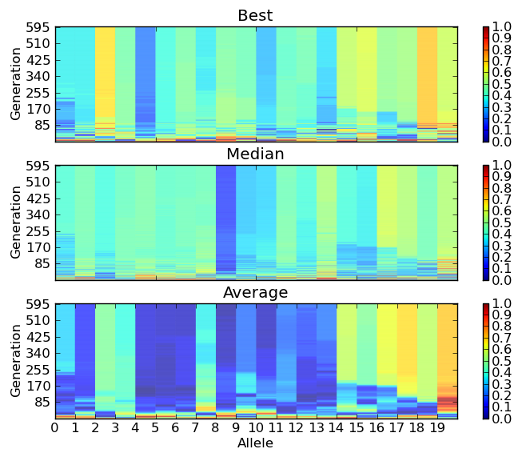
\includegraphics{allele_plot.png}
\caption{An example image saved from the \code{allele\_plot} function.}\end{figure}

Arguments:
\begin{itemize}
\item {} 
\emph{filename} -- the name of the individuals file produced by the file\_observer

\item {} 
\emph{normalize} -- Boolean value stating whether allele values should be
normalized before plotting (default False)

\item {} 
\emph{alleles} -- a list of allele index values that should be plotted
(default None)

\item {} 
\emph{generations} -- a list of generation numbers that should be plotted
(default None)

\end{itemize}

If \emph{alleles} is \code{None}, then all alleles are plotted. Similarly, if 
\emph{generations} is \code{None}, then all generations are plotted.

\end{fulllineitems}

\index{fitness\_statistics() (in module inspyred.ec.analysis)}

\begin{fulllineitems}
\phantomsection\label{reference:inspyred.ec.analysis.fitness_statistics}\pysiglinewithargsret{\code{inspyred.ec.analysis.}\bfcode{fitness\_statistics}}{\emph{population}}{}
Return the basic statistics of the population's fitness values.

This function returns a dictionary containing the ``best'', ``worst'',
``mean'', ``median'', and ``std'' fitness values in the population.
(``std'' is the standard deviation.) A typical usage would be similar
to the following:

\begin{Verbatim}[commandchars=\\\{\}]
\PYG{n}{stats} \PYG{o}{=} \PYG{n}{fitness\PYGZus{}statistics}\PYG{p}{(}\PYG{n}{population}\PYG{p}{)}
\PYG{k}{print}\PYG{p}{(}\PYG{n}{stats}\PYG{p}{[}\PYG{l+s}{'}\PYG{l+s}{best}\PYG{l+s}{'}\PYG{p}{]}\PYG{p}{)}
\PYG{k}{print}\PYG{p}{(}\PYG{n}{stats}\PYG{p}{[}\PYG{l+s}{'}\PYG{l+s}{worst}\PYG{l+s}{'}\PYG{p}{]}\PYG{p}{)}
\PYG{k}{print}\PYG{p}{(}\PYG{n}{stats}\PYG{p}{[}\PYG{l+s}{'}\PYG{l+s}{mean}\PYG{l+s}{'}\PYG{p}{]}\PYG{p}{)}
\PYG{k}{print}\PYG{p}{(}\PYG{n}{stats}\PYG{p}{[}\PYG{l+s}{'}\PYG{l+s}{median}\PYG{l+s}{'}\PYG{p}{]}\PYG{p}{)}
\PYG{k}{print}\PYG{p}{(}\PYG{n}{stats}\PYG{p}{[}\PYG{l+s}{'}\PYG{l+s}{std}\PYG{l+s}{'}\PYG{p}{]}\PYG{p}{)}
\end{Verbatim}

\begin{notice}{note}{Note:}
This function makes use of the numpy library for calculations. If that
library is not found, it attempts to complete the calculations 
internally. However, this second attempt will fail for multiobjective
fitness values and will return \code{nan} for the mean, median, and 
standard deviation.
\end{notice}

Arguments:
\begin{itemize}
\item {} 
\emph{population} -- the population of individuals

\end{itemize}

\end{fulllineitems}

\index{generation\_plot() (in module inspyred.ec.analysis)}

\begin{fulllineitems}
\phantomsection\label{reference:inspyred.ec.analysis.generation_plot}\pysiglinewithargsret{\code{inspyred.ec.analysis.}\bfcode{generation\_plot}}{\emph{filename}, \emph{errorbars=True}}{}
Plot the results of the algorithm using generation statistics.

This function creates a plot of the generation fitness statistics 
(best, worst, median, and average). This function requires the 
pylab and matplotlib libraries.

\begin{notice}{note}{Note:}
This function only works for single-objective problems.
\end{notice}
\begin{figure}[htbp]
\centering
\capstart

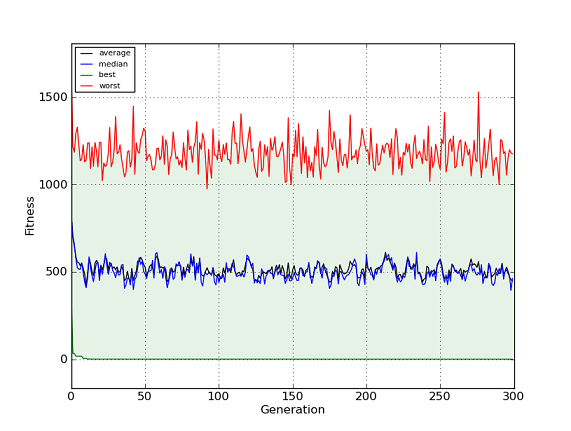
\includegraphics{generation_plot.png}
\caption{An example image saved from the \code{generation\_plot} function (without error bars).}\end{figure}

Arguments:
\begin{itemize}
\item {} 
\emph{filename} -- the name of the statistics file produced by the file\_observer

\item {} 
\emph{errorbars} -- Boolean value stating whether standard error bars should 
be drawn (default True)

\end{itemize}

\end{fulllineitems}

\index{hypervolume() (in module inspyred.ec.analysis)}

\begin{fulllineitems}
\phantomsection\label{reference:inspyred.ec.analysis.hypervolume}\pysiglinewithargsret{\code{inspyred.ec.analysis.}\bfcode{hypervolume}}{\emph{pareto\_set}, \emph{reference\_point=None}}{}
Calculates the hypervolume by slicing objectives (HSO).

This function calculates the hypervolume (or S-measure) of a nondominated
set using the Hypervolume by Slicing Objectives (HSO) procedure of \href{http://www.lania.mx/~ccoello/EMOO/while05a.pdf.gz}{While, et al. 
(IEEE CEC 2005)}.
The \emph{pareto\_set} should be a list of lists of objective values.
The \emph{reference\_point} may be specified or it may be left as the default 
value of None. In that case, the reference point is calculated to be the
maximum value in the set for all objectives (the ideal point). This function 
assumes that objectives are to be maximized.

Arguments:
\begin{itemize}
\item {} 
\emph{pareto\_set} -- the list or lists of objective values comprising the Pareto front

\item {} 
\emph{reference\_point} -- the reference point to be used (default None)

\end{itemize}

\end{fulllineitems}

\phantomsection\label{reference:module-inspyred.ec.utilities}\index{inspyred.ec.utilities (module)}

\subsection{\texttt{utilities} -- Optimization utility functions}
\label{reference:utilities-optimization-utility-functions}
This module provides utility classes and decorators for evolutionary computations.
\phantomsection\label{reference:module-utilities}\index{utilities (module)}\index{Objectify (class in inspyred.ec.utilities)}

\begin{fulllineitems}
\phantomsection\label{reference:inspyred.ec.utilities.Objectify}\pysiglinewithargsret{\strong{class }\code{inspyred.ec.utilities.}\bfcode{Objectify}}{\emph{func}}{}
Create an ``objectified'' version of a function.

This function allows an ordinary function passed to it to 
become essentially a callable instance of a class. For inspyred, 
this means that evolutionary operators (selectors, variators,
replacers, etc.) can be created as normal functions and then
be given the ability to have attributes \emph{that are specific to
the object}. Python functions can always have attributes without
employing any special mechanism, but those attributes exist for the 
function, and there is no way to create a new ``object'' except
by implementing a new function with the same functionality.
This class provides a way to ``objectify'' the same function
multiple times in order to provide each ``object'' with its own
set of independent attributes.

The attributes that are created on an objectified function are
passed into that function via the ubiquitous \code{args} variable
in inspyred. Any user-specified attributes are added to the 
\code{args} dictionary and replace any existing entry if necessary.
If the function modifies those entries in the dictionary (e.g.,
when dynamically modifying parameters), the corresponding 
attributes are modified as well.

Essentially, a local copy of the \code{args} dictionary is created
into which the attributes are inserted. This modified local copy 
is then passed to the function. After the function returns, the
values of the attributes from the dictionary are retrieved and 
are used to update the class attributes.

The typical usage is as follows:

\begin{Verbatim}[commandchars=\\\{\}]
\PYG{k}{def} \PYG{n+nf}{typical\PYGZus{}function}\PYG{p}{(}\PYG{o}{*}\PYG{n}{args}\PYG{p}{,} \PYG{o}{*}\PYG{o}{*}\PYG{n}{kwargs}\PYG{p}{)}\PYG{p}{:}
    \PYG{c}{\PYGZsh{} Implementation of typical function}
    \PYG{k}{pass}

\PYG{n}{fun\PYGZus{}one} \PYG{o}{=} \PYG{n}{Objectify}\PYG{p}{(}\PYG{n}{typical\PYGZus{}function}\PYG{p}{)}
\PYG{n}{fun\PYGZus{}two} \PYG{o}{=} \PYG{n}{Objectify}\PYG{p}{(}\PYG{n}{typical\PYGZus{}function}\PYG{p}{)}
\PYG{n}{fun\PYGZus{}one}\PYG{o}{.}\PYG{n}{attribute} \PYG{o}{=} \PYG{n}{value\PYGZus{}one}
\PYG{n}{fun\PYGZus{}two}\PYG{o}{.}\PYG{n}{attribute} \PYG{o}{=} \PYG{n}{value\PYGZus{}two}
\end{Verbatim}

\end{fulllineitems}

\index{memoize() (in module inspyred.ec.utilities)}

\begin{fulllineitems}
\phantomsection\label{reference:inspyred.ec.utilities.memoize}\pysiglinewithargsret{\code{inspyred.ec.utilities.}\bfcode{memoize}}{\emph{func=None}, \emph{maxlen=None}}{}
Cache a function's return value each time it is called.

This function serves as a function decorator to provide a caching of
evaluated fitness values. If called later with the same arguments, 
the cached value is returned instead of being re-evaluated.

This decorator assumes that candidates are individually pickleable, 
and their pickled values are used for hashing into a dictionary. It 
should be used when evaluating an \emph{expensive} fitness 
function to avoid costly re-evaluation of those fitnesses. The 
typical usage is as follows:

\begin{Verbatim}[commandchars=\\\{\}]
\PYG{n+nd}{@memoize}
\PYG{k}{def} \PYG{n+nf}{expensive\PYGZus{}fitness\PYGZus{}function}\PYG{p}{(}\PYG{n}{candidates}\PYG{p}{,} \PYG{n}{args}\PYG{p}{)}\PYG{p}{:}
    \PYG{c}{\PYGZsh{} Implementation of expensive fitness calculation}
    \PYG{k}{pass}
\end{Verbatim}

It is also possible to provide the named argument \emph{maxlen}, which
specifies the size of the memoization cache to use. (If \emph{maxlen} is
\code{None}, then an unbounded cache is used.) Once the size of the cache 
has reached \emph{maxlen}, the oldest element is replaced by the newest
element in order to keep the size constant. This usage is as follows:

\begin{Verbatim}[commandchars=\\\{\}]
\PYG{n+nd}{@memoize}\PYG{p}{(}\PYG{n}{maxlen}\PYG{o}{=}\PYG{l+m+mi}{100}\PYG{p}{)}
\PYG{k}{def} \PYG{n+nf}{expensive\PYGZus{}fitness\PYGZus{}function}\PYG{p}{(}\PYG{n}{candidates}\PYG{p}{,} \PYG{n}{args}\PYG{p}{)}\PYG{p}{:}
    \PYG{c}{\PYGZsh{} Implementation of expensive fitness calculation}
    \PYG{k}{pass}
\end{Verbatim}

\begin{notice}{warning}{Warning:}
The \code{maxlen} parameter must be passed as a named keyword
argument, or an \code{AttributeError} will be raised (e.g., saying 
\code{@memoize(100)} will cause an error).
\end{notice}

\end{fulllineitems}



\subsection{Operators}
\label{reference:operators}
An evolutionary computation is composed of many parts:
\begin{itemize}
\item {} 
an archiver -- stores solutions separate from the population (e.g., in a multiobjective EC)

\item {} 
an evaluator -- measures the fitness of candidate solutions; problem-dependent

\item {} 
a generator -- creates new candidate solutions; problem-dependent

\item {} 
a migrator -- moves individuals to other populations (in the case of distributed ECs)

\item {} 
observers -- view the progress of an EC in operation; may be a list of observers

\item {} 
a replacer -- determines the survivors of a generation

\item {} 
a selector -- determines the parents of a generation

\item {} 
terminators -- determine whether the evolution should stop; may be a list of terminators

\item {} 
variators -- modify candidate solutions; may be a list of variators

\end{itemize}

Each of these parts may be specified to create custom ECs to suit particular problems.
\phantomsection\label{reference:module-inspyred.ec.archivers}\index{inspyred.ec.archivers (module)}

\subsubsection{\texttt{archivers} -- Solution archival methods}
\label{reference:archivers-solution-archival-methods}
This module provides pre-defined archivers for evoluationary computations.

All archiver functions have the following arguments:
\begin{itemize}
\item {} 
\emph{random} -- the random number generator object

\item {} 
\emph{population} -- the population of individuals

\item {} 
\emph{archive} -- the current archive of individuals

\item {} 
\emph{args} -- a dictionary of keyword arguments

\end{itemize}

Each archiver function returns the updated archive.

\begin{notice}{note}{Note:}
The \emph{population} is really a shallow copy of the actual population of
the evolutionary computation. This means that any activities like
sorting will not affect the actual population.
\end{notice}
\phantomsection\label{reference:module-archivers}\index{archivers (module)}\index{adaptive\_grid\_archiver() (in module inspyred.ec.archivers)}

\begin{fulllineitems}
\phantomsection\label{reference:inspyred.ec.archivers.adaptive_grid_archiver}\pysiglinewithargsret{\code{inspyred.ec.archivers.}\bfcode{adaptive\_grid\_archiver}}{\emph{random}, \emph{population}, \emph{archive}, \emph{args}}{}
Archive only the best individual(s) using a fixed size grid.

This function archives the best solutions by using a fixed-size grid
to determine which existing solutions should be removed in order to
make room for new ones. This archiver is designed specifically for
use with the Pareto Archived Evolution Strategy (PAES).

Optional keyword arguments in args:
\begin{itemize}
\item {} 
\emph{max\_archive\_size} -- the maximum number of individuals in the archive
(default len(population))

\item {} 
\emph{num\_grid\_divisions} -- the number of grid divisions (default 1)

\end{itemize}

\end{fulllineitems}

\index{best\_archiver() (in module inspyred.ec.archivers)}

\begin{fulllineitems}
\phantomsection\label{reference:inspyred.ec.archivers.best_archiver}\pysiglinewithargsret{\code{inspyred.ec.archivers.}\bfcode{best\_archiver}}{\emph{random}, \emph{population}, \emph{archive}, \emph{args}}{}
Archive only the best individual(s).

This function archives the best solutions and removes inferior ones.
If the comparison operators have been overloaded to define Pareto
preference (as in the \code{Pareto} class), then this archiver will form 
a Pareto archive.

\end{fulllineitems}

\index{default\_archiver() (in module inspyred.ec.archivers)}

\begin{fulllineitems}
\phantomsection\label{reference:inspyred.ec.archivers.default_archiver}\pysiglinewithargsret{\code{inspyred.ec.archivers.}\bfcode{default\_archiver}}{\emph{random}, \emph{population}, \emph{archive}, \emph{args}}{}
Do nothing.

This function just returns the existing archive (which is
probably empty) with no changes.

\end{fulllineitems}

\index{population\_archiver() (in module inspyred.ec.archivers)}

\begin{fulllineitems}
\phantomsection\label{reference:inspyred.ec.archivers.population_archiver}\pysiglinewithargsret{\code{inspyred.ec.archivers.}\bfcode{population\_archiver}}{\emph{random}, \emph{population}, \emph{archive}, \emph{args}}{}
Archive the current population.

This function replaces the archive with the individuals 
of the current population.

\end{fulllineitems}

\phantomsection\label{reference:module-inspyred.ec.evaluators}\index{inspyred.ec.evaluators (module)}

\subsubsection{\texttt{evaluators} -- Fitness evaluation methods}
\label{reference:evaluators-fitness-evaluation-methods}
Evaluator functions are problem-specific. This module provides pre-defined 
evaluators for evolutionary computations.

All evaluator functions have the following arguments:
\begin{itemize}
\item {} 
\emph{candidates} -- the candidate solutions

\item {} 
\emph{args} -- a dictionary of keyword arguments

\end{itemize}
\phantomsection\label{reference:module-evaluators}\index{evaluators (module)}\index{evaluator() (in module inspyred.ec.evaluators)}

\begin{fulllineitems}
\phantomsection\label{reference:inspyred.ec.evaluators.evaluator}\pysiglinewithargsret{\code{inspyred.ec.evaluators.}\bfcode{evaluator}}{\emph{evaluate}}{}
Return an inspyred evaluator function based on the given function.

This function generator takes a function that evaluates only one
candidate. The generator handles the iteration over each candidate 
to be evaluated.

The given function \code{evaluate} must have the following signature:

\begin{Verbatim}[commandchars=\\\{\}]
\PYG{n}{fitness} \PYG{o}{=} \PYG{n}{evaluate}\PYG{p}{(}\PYG{n}{candidate}\PYG{p}{,} \PYG{n}{args}\PYG{p}{)}
\end{Verbatim}

This function is most commonly used as a function decorator with
the following usage:

\begin{Verbatim}[commandchars=\\\{\}]
\PYG{n+nd}{@evaluator}
\PYG{k}{def} \PYG{n+nf}{evaluate}\PYG{p}{(}\PYG{n}{candidate}\PYG{p}{,} \PYG{n}{args}\PYG{p}{)}\PYG{p}{:}
    \PYG{c}{\PYGZsh{} Implementation of evaluation}
    \PYG{k}{pass}
\end{Verbatim}

The generated function also contains an attribute named
\code{single\_evaluation} which holds the original evaluation function.
In this way, the original single-candidate function can be
retrieved if necessary.

\end{fulllineitems}

\index{parallel\_evaluation\_mp() (in module inspyred.ec.evaluators)}

\begin{fulllineitems}
\phantomsection\label{reference:inspyred.ec.evaluators.parallel_evaluation_mp}\pysiglinewithargsret{\code{inspyred.ec.evaluators.}\bfcode{parallel\_evaluation\_mp}}{\emph{candidates}, \emph{args}}{}
Evaluate the candidates in parallel using \code{multiprocessing}.

This function allows parallel evaluation of candidate solutions.
It uses the standard multiprocessing library to accomplish the 
parallelization. The function assigns the evaluation of each
candidate to its own job, all of which are then distributed to the
available processing units.

\begin{notice}{note}{Note:}
All arguments to the evaluation function must be pickleable.
Those that are not will not be sent through the \code{args} variable
and will be unavailable to your function.
\end{notice}

Required keyword arguments in args:
\begin{itemize}
\item {} 
\emph{mp\_evaluator} -- actual evaluation function to be used (This function
should have the same signature as any other inspyred evaluation function.)

\end{itemize}

Optional keyword arguments in args:
\begin{itemize}
\item {} 
\emph{mp\_nprocs} -- number of processors that will be used (default machine 
cpu count)

\end{itemize}

\end{fulllineitems}

\index{parallel\_evaluation\_pp() (in module inspyred.ec.evaluators)}

\begin{fulllineitems}
\phantomsection\label{reference:inspyred.ec.evaluators.parallel_evaluation_pp}\pysiglinewithargsret{\code{inspyred.ec.evaluators.}\bfcode{parallel\_evaluation\_pp}}{\emph{candidates}, \emph{args}}{}
Evaluate the candidates in parallel using Parallel Python.

This function allows parallel evaluation of candidate solutions.
It uses the \href{http://www.parallelpython.com}{Parallel Python}  (pp)
library to accomplish the parallelization. This library must already 
be installed in order to use this function. The function assigns the 
evaluation of each candidate to its own job, all of which are then 
distributed to the available processing units.

\begin{notice}{note}{Note:}
All arguments to the evaluation function must be pickleable.
Those that are not will not be sent through the \code{args} variable
and will be unavailable to your function.
\end{notice}

Required keyword arguments in args:
\begin{itemize}
\item {} 
\emph{pp\_evaluator} -- actual evaluation function to be used (This function
should have the same signature as any other inspyred evaluation function.)

\end{itemize}

Optional keyword arguments in args:
\begin{itemize}
\item {} 
\emph{pp\_dependencies} -- tuple of functional dependencies of the serial 
evaluator (default ())

\item {} 
\emph{pp\_modules} -- tuple of modules that must be imported for the 
functional dependencies (default ())

\item {} 
\emph{pp\_servers} -- tuple of servers (on a cluster) that will be used 
for parallel processing (default (``*'',))

\item {} 
\emph{pp\_secret} -- string representing the secret key needed to authenticate
on a worker node (default ``inspyred'')

\item {} 
\emph{pp\_nprocs} -- integer representing the number of worker processes to
start on the local machine (default ``autodetect'', which sets it to the
number of processors in the system)

\end{itemize}

For more information about these arguments, please consult the
documentation for \href{http://www.parallelpython.com}{Parallel Python}.

\end{fulllineitems}

\phantomsection\label{reference:module-inspyred.ec.generators}\index{inspyred.ec.generators (module)}

\subsubsection{\texttt{generators} -- Solution generation methods}
\label{reference:generators-solution-generation-methods}
Generator functions are problem-specific. They are used to create the 
initial set of candidate solutions needed by the evolutionary computation.

All generator functions have the following arguments:
\begin{itemize}
\item {} 
\emph{random} -- the random number generator object

\item {} 
\emph{args} -- a dictionary of keyword arguments

\end{itemize}
\phantomsection\label{reference:module-generators}\index{generators (module)}\index{diversify (class in inspyred.ec.generators)}

\begin{fulllineitems}
\phantomsection\label{reference:inspyred.ec.generators.diversify}\pysiglinewithargsret{\strong{class }\code{inspyred.ec.generators.}\bfcode{diversify}}{\emph{generator}}{}
Ensure uniqueness of candidates created by a generator.

This function decorator is used to enforce uniqueness of candidates 
created by a generator. The decorator maintains a list of previously
created candidates, and it ensures that new candidates are unique by
checking a generated candidate against that list, regenerating if a
duplicate is found. The typical usage is as follows:

\begin{Verbatim}[commandchars=\\\{\}]
\PYG{n+nd}{@diversify}
\PYG{k}{def} \PYG{n+nf}{generator\PYGZus{}function}\PYG{p}{(}\PYG{n}{random}\PYG{p}{,} \PYG{n}{args}\PYG{p}{)}\PYG{p}{:}
    \PYG{c}{\PYGZsh{} Normal generator function}
    \PYG{k}{pass}
\end{Verbatim}

If a list of seeds is used, then these can be specified prior to the
generator's use by saying the following:

\begin{Verbatim}[commandchars=\\\{\}]
\PYG{n+nd}{@diversify}
\PYG{k}{def} \PYG{n+nf}{generator\PYGZus{}function}\PYG{p}{(}\PYG{n}{random}\PYG{p}{,} \PYG{n}{args}\PYG{p}{)}\PYG{p}{:}
    \PYG{c}{\PYGZsh{} Normal generator function}
    \PYG{k}{pass}
\PYG{n}{generator\PYGZus{}function}\PYG{o}{.}\PYG{n}{candidates} \PYG{o}{=} \PYG{n}{seeds}
\end{Verbatim}

\end{fulllineitems}

\index{strategize() (in module inspyred.ec.generators)}

\begin{fulllineitems}
\phantomsection\label{reference:inspyred.ec.generators.strategize}\pysiglinewithargsret{\code{inspyred.ec.generators.}\bfcode{strategize}}{\emph{generator}}{}
Add strategy parameters to candidates created by a generator.

This function decorator is used to provide a means of adding strategy 
parameters to candidates created by a generator. The generator function 
is modifed to extend the candidate with \code{len(candidate)} strategy 
parameters (one per candidate element). Each strategy parameter is 
initialized to a random value in the range {[}0, 1{]}. The typical usage is 
as follows:

\begin{Verbatim}[commandchars=\\\{\}]
\PYG{n+nd}{@strategize}
\PYG{k}{def} \PYG{n+nf}{generator\PYGZus{}function}\PYG{p}{(}\PYG{n}{random}\PYG{p}{,} \PYG{n}{args}\PYG{p}{)}\PYG{p}{:}
    \PYG{c}{\PYGZsh{} Normal generator function}
    \PYG{k}{pass}
\end{Verbatim}

\end{fulllineitems}

\phantomsection\label{reference:module-inspyred.ec.migrators}\index{inspyred.ec.migrators (module)}

\subsubsection{\texttt{migrators} -- Solution migration methods}
\label{reference:migrators-solution-migration-methods}
This module provides pre-defined migrators for evolutionary computations.

All migrator functions have the following arguments:
\begin{itemize}
\item {} 
\emph{random} -- the random number generator object

\item {} 
\emph{population} -- the population of Individuals

\item {} 
\emph{args} -- a dictionary of keyword arguments

\end{itemize}

Each migrator function returns the updated population.

Migrator functions would typically be used for multi-population approaches,
such as island-model evolutionary computations. They provide a means for
individuals to be transferred from one population to another during the
evolutionary process.
\phantomsection\label{reference:module-migrators}\index{migrators (module)}\index{MultiprocessingMigrator (class in inspyred.ec.migrators)}

\begin{fulllineitems}
\phantomsection\label{reference:inspyred.ec.migrators.MultiprocessingMigrator}\pysiglinewithargsret{\strong{class }\code{inspyred.ec.migrators.}\bfcode{MultiprocessingMigrator}}{\emph{max\_migrants=1}}{}
Migrate among processes on the same machine.

This callable class allows individuals to migrate from one process 
to another on the same machine. It maintains a queue of migrants
whose maximum length can be fixed via the \code{max\_migrants}
parameter in the constructor. If the number of migrants in the queue
reaches this value, new migrants are not added until earlier ones
are consumed. The unreliability of a multiprocessing environment
makes it difficult to provide guarantees. However, migrants are 
theoretically added and consumed at the same rate, so this value
should determine the ``freshness'' of individuals, where smaller
queue sizes provide more recency.

An optional keyword argument in \code{args} requires the migrant to be
evaluated by the current evolutionary computation before being inserted 
into the population. This can be important when different populations 
use different evaluation functions and you need to be able to compare 
``apples with apples,'' so to speak.

Optional keyword arguments in args:
\begin{itemize}
\item {} 
\emph{evaluate\_migrant} -- should new migrants be evaluated before 
adding them to the population (default False)

\end{itemize}

\end{fulllineitems}

\index{default\_migration() (in module inspyred.ec.migrators)}

\begin{fulllineitems}
\phantomsection\label{reference:inspyred.ec.migrators.default_migration}\pysiglinewithargsret{\code{inspyred.ec.migrators.}\bfcode{default\_migration}}{\emph{random}, \emph{population}, \emph{args}}{}
Do nothing.

This function just returns the existing population with no changes.

\end{fulllineitems}

\phantomsection\label{reference:module-inspyred.ec.observers}\index{inspyred.ec.observers (module)}

\subsubsection{\texttt{observers} -- Algorithm monitoring methods}
\label{reference:observers-algorithm-monitoring-methods}
This module provides pre-defined observers for evolutionary computations.

All observer functions have the following arguments:
\begin{itemize}
\item {} 
\emph{population} -- the population of Individuals

\item {} 
\emph{num\_generations} -- the number of elapsed generations

\item {} 
\emph{num\_evaluations} -- the number of candidate solution evaluations

\item {} 
\emph{args} -- a dictionary of keyword arguments

\end{itemize}

\begin{notice}{note}{Note:}
The \emph{population} is really a shallow copy of the actual population of
the evolutionary computation. This means that any activities like
sorting will not affect the actual population.
\end{notice}
\phantomsection\label{reference:module-observers}\index{observers (module)}\index{EmailObserver (class in inspyred.ec.observers)}

\begin{fulllineitems}
\phantomsection\label{reference:inspyred.ec.observers.EmailObserver}\pysiglinewithargsret{\strong{class }\code{inspyred.ec.observers.}\bfcode{EmailObserver}}{\emph{username}, \emph{password}, \emph{server}, \emph{port=587}}{}
Email the population statistics, individuals, and optional file observer data.

This callable class allows information about the current generation
to be emailed to a user. This is useful when dealing with computationally
expensive optimization problems where the evolution must progress over
hours or days. The \code{generation\_step} attribute can be set to an integer
greater than 1 to ensure that emails are only sent on generations that are
multiples of the step size.

\begin{notice}{note}{Note:}
This function makes use of the \code{inspyred.ec.analysis.fitness\_statistics} 
function, so it is subject to the same requirements.
\end{notice}

A typical instantiation of this class would be the following:

\begin{Verbatim}[commandchars=\\\{\}]
\PYG{k+kn}{import} \PYG{n+nn}{getpass}
\PYG{n}{usr} \PYG{o}{=} \PYG{n+nb}{raw\PYGZus{}input}\PYG{p}{(}\PYG{l+s}{"}\PYG{l+s}{Enter your username: }\PYG{l+s}{"}\PYG{p}{)}
\PYG{n}{pwd} \PYG{o}{=} \PYG{n}{getpass}\PYG{o}{.}\PYG{n}{getpass}\PYG{p}{(}\PYG{l+s}{"}\PYG{l+s}{Enter your password: }\PYG{l+s}{"}\PYG{p}{)}
\PYG{n}{email\PYGZus{}observer} \PYG{o}{=} \PYG{n}{EmailObserver}\PYG{p}{(}\PYG{n}{usr}\PYG{p}{,} \PYG{n}{pwd}\PYG{p}{,} \PYG{l+s}{"}\PYG{l+s}{my.mail.server}\PYG{l+s}{"}\PYG{p}{)}
\PYG{n}{email\PYGZus{}observer}\PYG{o}{.}\PYG{n}{from\PYGZus{}address} \PYG{o}{=} \PYG{l+s}{"}\PYG{l+s}{me@here.com}\PYG{l+s}{"}
\PYG{n}{email\PYGZus{}observer}\PYG{o}{.}\PYG{n}{to\PYGZus{}address} \PYG{o}{=} \PYG{l+s}{"}\PYG{l+s}{you@there.com}\PYG{l+s}{"} \PYG{c}{\PYGZsh{} or ["you@there.com", "other@somewhere.com"]}
\PYG{n}{email\PYGZus{}observer}\PYG{o}{.}\PYG{n}{subject} \PYG{o}{=} \PYG{l+s}{"}\PYG{l+s}{My custom subject}\PYG{l+s}{"}
\PYG{n}{email\PYGZus{}observer}\PYG{o}{.}\PYG{n}{generation\PYGZus{}step} \PYG{o}{=} \PYG{l+m+mi}{10} \PYG{c}{\PYGZsh{} Send an email every 10th generation}
\end{Verbatim}

Public Attributes:
\begin{itemize}
\item {} 
\emph{username} -- the mail server username

\item {} 
\emph{password} -- the mail server password

\item {} 
\emph{server} -- the mail server URL or IP address string

\item {} 
\emph{port} -- the mail server port as an integer

\item {} 
\emph{from\_address} -- the email address of the sender

\item {} 
\emph{to\_address} -- the (possibly list of) email address(es) of the receiver(s)

\item {} 
\emph{subject} -- the subject of the email (default `inspyred observer report')

\item {} 
\emph{max\_attachment} -- the maximum allowable size, in MB, of attachments
(default 20 MB)

\item {} 
\emph{generation\_step} -- the step size for when a generation's information 
should be emailed (default 1)

\end{itemize}

\end{fulllineitems}

\index{archive\_observer() (in module inspyred.ec.observers)}

\begin{fulllineitems}
\phantomsection\label{reference:inspyred.ec.observers.archive_observer}\pysiglinewithargsret{\code{inspyred.ec.observers.}\bfcode{archive\_observer}}{\emph{population}, \emph{num\_generations}, \emph{num\_evaluations}, \emph{args}}{}
Print the current archive to the screen.

This function displays the current archive of the evolutionary 
computation to the screen.

\end{fulllineitems}

\index{best\_observer() (in module inspyred.ec.observers)}

\begin{fulllineitems}
\phantomsection\label{reference:inspyred.ec.observers.best_observer}\pysiglinewithargsret{\code{inspyred.ec.observers.}\bfcode{best\_observer}}{\emph{population}, \emph{num\_generations}, \emph{num\_evaluations}, \emph{args}}{}
Print the best individual in the population to the screen.

This function displays the best individual in the population to 
the screen.

\end{fulllineitems}

\index{default\_observer() (in module inspyred.ec.observers)}

\begin{fulllineitems}
\phantomsection\label{reference:inspyred.ec.observers.default_observer}\pysiglinewithargsret{\code{inspyred.ec.observers.}\bfcode{default\_observer}}{\emph{population}, \emph{num\_generations}, \emph{num\_evaluations}, \emph{args}}{}
Do nothing.

\end{fulllineitems}

\index{file\_observer() (in module inspyred.ec.observers)}

\begin{fulllineitems}
\phantomsection\label{reference:inspyred.ec.observers.file_observer}\pysiglinewithargsret{\code{inspyred.ec.observers.}\bfcode{file\_observer}}{\emph{population}, \emph{num\_generations}, \emph{num\_evaluations}, \emph{args}}{}
Print the output of the evolutionary computation to a file.

This function saves the results of the evolutionary computation
to two files. The first file, which by default is named 
`inspyred-statistics-file-\textless{}timestamp\textgreater{}.csv', contains the basic
generational statistics of the population throughout the run
(worst, best, median, and average fitness and standard deviation
of the fitness values). The second file, which by default is named
`inspyred-individuals-file-\textless{}timestamp\textgreater{}.csv', contains every individual
during each generation of the run. Both files may be passed to the
function as keyword arguments (see below).

The format of each line of the statistics file is as follows:

\begin{Verbatim}[commandchars=\\\{\}]
generation number, population size, worst, best, median, average, standard deviation
\end{Verbatim}

The format of each line of the individuals file is as follows:

\begin{Verbatim}[commandchars=\\\{\}]
generation number, individual number, fitness, string representation of candidate
\end{Verbatim}

\begin{notice}{note}{Note:}
This function makes use of the \code{inspyred.ec.analysis.fitness\_statistics} 
function, so it is subject to the same requirements.
\end{notice}

Optional keyword arguments in args:
\begin{itemize}
\item {} 
\emph{statistics\_file} -- a file object (default: see text)

\item {} 
\emph{individuals\_file} -- a file object (default: see text)

\end{itemize}

\end{fulllineitems}

\index{plot\_observer() (in module inspyred.ec.observers)}

\begin{fulllineitems}
\phantomsection\label{reference:inspyred.ec.observers.plot_observer}\pysiglinewithargsret{\code{inspyred.ec.observers.}\bfcode{plot\_observer}}{\emph{population}, \emph{num\_generations}, \emph{num\_evaluations}, \emph{args}}{}
Plot the output of the evolutionary computation as a graph.

This function plots the performance of the EC as a line graph 
using the pylab library (matplotlib) and numpy. The graph consists of a 
blue line representing the best fitness, a green line representing
the average fitness, and a red line representing the median fitness.
It modifies the keyword arguments variable `args' by including an
entry called `plot\_data'.

If this observer is used, the calling script should also import
the pylab library and should end the script with

pylab.show()

Otherwise, the program may generate a runtime error.

\begin{notice}{note}{Note:}
This function makes use of the pylab and numpy libraries.
\end{notice}

\end{fulllineitems}

\index{population\_observer() (in module inspyred.ec.observers)}

\begin{fulllineitems}
\phantomsection\label{reference:inspyred.ec.observers.population_observer}\pysiglinewithargsret{\code{inspyred.ec.observers.}\bfcode{population\_observer}}{\emph{population}, \emph{num\_generations}, \emph{num\_evaluations}, \emph{args}}{}
Print the current population of the evolutionary computation to the screen.

This function displays the current population of the evolutionary 
computation to the screen in fitness-sorted order.

\end{fulllineitems}

\index{stats\_observer() (in module inspyred.ec.observers)}

\begin{fulllineitems}
\phantomsection\label{reference:inspyred.ec.observers.stats_observer}\pysiglinewithargsret{\code{inspyred.ec.observers.}\bfcode{stats\_observer}}{\emph{population}, \emph{num\_generations}, \emph{num\_evaluations}, \emph{args}}{}
Print the statistics of the evolutionary computation to the screen.

This function displays the statistics of the evolutionary computation
to the screen. The output includes the generation number, the current
number of evaluations, the maximum fitness, the minimum fitness, 
the average fitness, and the standard deviation.

\begin{notice}{note}{Note:}
This function makes use of the \code{inspyred.ec.analysis.fitness\_statistics} 
function, so it is subject to the same requirements.
\end{notice}

\end{fulllineitems}

\phantomsection\label{reference:module-inspyred.ec.replacers}\index{inspyred.ec.replacers (module)}

\subsubsection{\texttt{replacers} -- Survivor replacement methods}
\label{reference:replacers-survivor-replacement-methods}
This module provides pre-defined replacers for evolutionary computations.

All replacer functions have the following arguments:
\begin{itemize}
\item {} 
\emph{random} -- the random number generator object

\item {} 
\emph{population} -- the population of individuals

\item {} 
\emph{parents} -- the list of parent individuals

\item {} 
\emph{offspring} -- the list of offspring individuals

\item {} 
\emph{args} -- a dictionary of keyword arguments

\end{itemize}

Each replacer function returns the list of surviving individuals.
\phantomsection\label{reference:module-replacers}\index{replacers (module)}\index{comma\_replacement() (in module inspyred.ec.replacers)}

\begin{fulllineitems}
\phantomsection\label{reference:inspyred.ec.replacers.comma_replacement}\pysiglinewithargsret{\code{inspyred.ec.replacers.}\bfcode{comma\_replacement}}{\emph{random}, \emph{population}, \emph{parents}, \emph{offspring}, \emph{args}}{}
Performs ``comma'' replacement.

This function performs ``comma'' replacement, which means that
the entire existing population is replaced by the best
population-many elements from the offspring. This function
makes the assumption that the size of the offspring is at 
least as large as the original population. Otherwise, the
population size will not be constant.

\end{fulllineitems}

\index{crowding\_replacement() (in module inspyred.ec.replacers)}

\begin{fulllineitems}
\phantomsection\label{reference:inspyred.ec.replacers.crowding_replacement}\pysiglinewithargsret{\code{inspyred.ec.replacers.}\bfcode{crowding\_replacement}}{\emph{random}, \emph{population}, \emph{parents}, \emph{offspring}, \emph{args}}{}
Performs crowding replacement as a form of niching.

This function performs crowding replacement, which means that
the members of the population are replaced one-at-a-time with
each of the offspring. A random sample of \emph{crowding\_distance}
individuals is pulled from the current population, and the
closest individual to the current offspring (where ``closest''
is determined by the \emph{distance\_function}) is replaced by that
offspring, if the offspring is better. It is possible for one 
offspring to replace an earlier offspring in the same generation, 
given the random sample that is taken of the current survivors 
for each offspring.

Optional keyword arguments in args:
\begin{itemize}
\item {} 
\emph{distance\_function} -- a function that accepts two candidate 
solutions and returns the distance between them (default 
Euclidean L2 distance)

\item {} 
\emph{crowding\_distance} -- a positive integer representing the 
number of closest solutions to consider as a ``crowd'' (default 2)

\end{itemize}

\end{fulllineitems}

\index{default\_replacement() (in module inspyred.ec.replacers)}

\begin{fulllineitems}
\phantomsection\label{reference:inspyred.ec.replacers.default_replacement}\pysiglinewithargsret{\code{inspyred.ec.replacers.}\bfcode{default\_replacement}}{\emph{random}, \emph{population}, \emph{parents}, \emph{offspring}, \emph{args}}{}
Performs no replacement, returning the original population.

\end{fulllineitems}

\index{generational\_replacement() (in module inspyred.ec.replacers)}

\begin{fulllineitems}
\phantomsection\label{reference:inspyred.ec.replacers.generational_replacement}\pysiglinewithargsret{\code{inspyred.ec.replacers.}\bfcode{generational\_replacement}}{\emph{random}, \emph{population}, \emph{parents}, \emph{offspring}, \emph{args}}{}
Performs generational replacement with optional weak elitism.

This function performs generational replacement, which means that
the entire existing population is replaced by the offspring,
truncating to the population size if the number of offspring is 
larger. Weak elitism may also be specified through the \emph{num\_elites}
keyword argument in args. If this is used, the best \emph{num\_elites}
individuals in the current population are allowed to survive if
they are better than the worst \emph{num\_elites} offspring.

Optional keyword arguments in args:
\begin{itemize}
\item {} 
\emph{num\_elites} -- number of elites to consider (default 0)

\end{itemize}

\end{fulllineitems}

\index{nsga\_replacement() (in module inspyred.ec.replacers)}

\begin{fulllineitems}
\phantomsection\label{reference:inspyred.ec.replacers.nsga_replacement}\pysiglinewithargsret{\code{inspyred.ec.replacers.}\bfcode{nsga\_replacement}}{\emph{random}, \emph{population}, \emph{parents}, \emph{offspring}, \emph{args}}{}
Replaces population using the non-dominated sorting technique from NSGA-II.

\end{fulllineitems}

\index{paes\_replacement() (in module inspyred.ec.replacers)}

\begin{fulllineitems}
\phantomsection\label{reference:inspyred.ec.replacers.paes_replacement}\pysiglinewithargsret{\code{inspyred.ec.replacers.}\bfcode{paes\_replacement}}{\emph{random}, \emph{population}, \emph{parents}, \emph{offspring}, \emph{args}}{}
Replaces population using the Pareto Archived Evolution Strategy method.

\end{fulllineitems}

\index{plus\_replacement() (in module inspyred.ec.replacers)}

\begin{fulllineitems}
\phantomsection\label{reference:inspyred.ec.replacers.plus_replacement}\pysiglinewithargsret{\code{inspyred.ec.replacers.}\bfcode{plus\_replacement}}{\emph{random}, \emph{population}, \emph{parents}, \emph{offspring}, \emph{args}}{}
Performs ``plus'' replacement.

This function performs ``plus'' replacement, which means that
the entire existing population is replaced by the best
population-many elements from the combined set of parents and 
offspring.

\end{fulllineitems}

\index{random\_replacement() (in module inspyred.ec.replacers)}

\begin{fulllineitems}
\phantomsection\label{reference:inspyred.ec.replacers.random_replacement}\pysiglinewithargsret{\code{inspyred.ec.replacers.}\bfcode{random\_replacement}}{\emph{random}, \emph{population}, \emph{parents}, \emph{offspring}, \emph{args}}{}
Performs random replacement with optional weak elitism.

This function performs random replacement, which means that
the offspring replace random members of the population, keeping
the population size constant. Weak elitism may also be specified 
through the \emph{num\_elites} keyword argument in args. If this is used, 
the best \emph{num\_elites} individuals in the current population are 
allowed to survive if they are better than the worst \emph{num\_elites}
offspring.

Optional keyword arguments in args:
\begin{itemize}
\item {} 
\emph{num\_elites} -- number of elites to consider (default 0)

\end{itemize}

\end{fulllineitems}

\index{simulated\_annealing\_replacement() (in module inspyred.ec.replacers)}

\begin{fulllineitems}
\phantomsection\label{reference:inspyred.ec.replacers.simulated_annealing_replacement}\pysiglinewithargsret{\code{inspyred.ec.replacers.}\bfcode{simulated\_annealing\_replacement}}{\emph{random}, \emph{population}, \emph{parents}, \emph{offspring}, \emph{args}}{}
Replaces population using the simulated annealing schedule.

This function performs simulated annealing replacement based
on a temperature and a cooling rate. These can be specified
by the keyword arguments \emph{temperature}, which should be the
initial temperature, and \emph{cooling\_rate}, which should be the
coefficient by which the temperature is reduced. If these
keyword arguments are not present, then the function will
attempt to base the cooling schedule either on the ratio of 
evaluations to the maximum allowed evaluations or on the 
ratio of generations to the maximum allowed generations. 
Each of these ratios is of the form \code{(max - current)/max}
so that the cooling schedule moves smoothly from 1 to 0.

Optional keyword arguments in args:
\begin{itemize}
\item {} 
\emph{temperature} -- the initial temperature

\item {} 
\emph{cooling\_rate} -- a real-valued coefficient in the range (0, 1) 
by which the temperature should be reduced

\end{itemize}

\end{fulllineitems}

\index{steady\_state\_replacement() (in module inspyred.ec.replacers)}

\begin{fulllineitems}
\phantomsection\label{reference:inspyred.ec.replacers.steady_state_replacement}\pysiglinewithargsret{\code{inspyred.ec.replacers.}\bfcode{steady\_state\_replacement}}{\emph{random}, \emph{population}, \emph{parents}, \emph{offspring}, \emph{args}}{}
Performs steady-state replacement for the offspring.

This function performs steady-state replacement, which means that
the offspring replace the least fit individuals in the existing
population, even if those offspring are less fit than the individuals
that they replace.

\end{fulllineitems}

\index{truncation\_replacement() (in module inspyred.ec.replacers)}

\begin{fulllineitems}
\phantomsection\label{reference:inspyred.ec.replacers.truncation_replacement}\pysiglinewithargsret{\code{inspyred.ec.replacers.}\bfcode{truncation\_replacement}}{\emph{random}, \emph{population}, \emph{parents}, \emph{offspring}, \emph{args}}{}
Replaces population with the best of the population and offspring.

This function performs truncation replacement, which means that
the entire existing population is replaced by the best from among
the current population and offspring, keeping the existing population
size fixed. This is similar to so-called ``plus'' replacement in the 
evolution strategies literature, except that ``plus'' replacement 
considers only parents and offspring for survival. However, if the
entire population are parents (which is often the case in evolution 
strategies), then truncation replacement and plus-replacement are 
equivalent approaches.

\end{fulllineitems}

\phantomsection\label{reference:module-inspyred.ec.selectors}\index{inspyred.ec.selectors (module)}

\subsubsection{\texttt{selectors} -- Parent selection methods}
\label{reference:selectors-parent-selection-methods}
This module provides pre-defined selectors for evolutionary computations.

All selector functions have the following arguments:
\begin{itemize}
\item {} 
\emph{random} -- the random number generator object

\item {} 
\emph{population} -- the population of individuals

\item {} 
\emph{args} -- a dictionary of keyword arguments

\end{itemize}

Each selector function returns the list of selected individuals.

\begin{notice}{note}{Note:}
The \emph{population} is really a shallow copy of the actual population of
the evolutionary computation. This means that any activities like
sorting will not affect the actual population.
\end{notice}
\phantomsection\label{reference:module-selectors}\index{selectors (module)}\index{default\_selection() (in module inspyred.ec.selectors)}

\begin{fulllineitems}
\phantomsection\label{reference:inspyred.ec.selectors.default_selection}\pysiglinewithargsret{\code{inspyred.ec.selectors.}\bfcode{default\_selection}}{\emph{random}, \emph{population}, \emph{args}}{}
Return the population.

This function acts as a default selection scheme for an evolutionary
computation. It simply returns the entire population as having been 
selected.

\end{fulllineitems}

\index{fitness\_proportionate\_selection() (in module inspyred.ec.selectors)}

\begin{fulllineitems}
\phantomsection\label{reference:inspyred.ec.selectors.fitness_proportionate_selection}\pysiglinewithargsret{\code{inspyred.ec.selectors.}\bfcode{fitness\_proportionate\_selection}}{\emph{random}, \emph{population}, \emph{args}}{}
Return fitness proportionate sampling of individuals from the population.

This function stochastically chooses individuals from the population
with probability proportional to their fitness. This is often 
referred to as ``roulette wheel'' selection. Note that this selection
is not valid for minimization problems.

Optional keyword arguments in args:
\begin{itemize}
\item {} 
\emph{num\_selected} -- the number of individuals to be selected (default 1)

\end{itemize}

\end{fulllineitems}

\index{rank\_selection() (in module inspyred.ec.selectors)}

\begin{fulllineitems}
\phantomsection\label{reference:inspyred.ec.selectors.rank_selection}\pysiglinewithargsret{\code{inspyred.ec.selectors.}\bfcode{rank\_selection}}{\emph{random}, \emph{population}, \emph{args}}{}
Return a rank-based sampling of individuals from the population.

This function behaves similarly to fitness proportionate selection,
except that it uses the individual's rank in the population, rather
than its raw fitness value, to determine its probability. This
means that it can be used for both maximization and minimization 
problems, since higher rank can be defined correctly for both.

Optional keyword arguments in args:
\begin{itemize}
\item {} 
\emph{num\_selected} -- the number of individuals to be selected (default 1)

\end{itemize}

\end{fulllineitems}

\index{tournament\_selection() (in module inspyred.ec.selectors)}

\begin{fulllineitems}
\phantomsection\label{reference:inspyred.ec.selectors.tournament_selection}\pysiglinewithargsret{\code{inspyred.ec.selectors.}\bfcode{tournament\_selection}}{\emph{random}, \emph{population}, \emph{args}}{}
Return a tournament sampling of individuals from the population.

This function selects \code{num\_selected} individuals from the population. 
It selects each one by using random sampling without replacement
to pull \code{tournament\_size} individuals and adds the best of the
tournament as its selection. If \code{tournament\_size} is greater than
the population size, the population size is used instead as the size
of the tournament.

Optional keyword arguments in args:
\begin{itemize}
\item {} 
\emph{num\_selected} -- the number of individuals to be selected (default 1)

\item {} 
\emph{tournament\_size} -- the tournament size (default 2)

\end{itemize}

\end{fulllineitems}

\index{truncation\_selection() (in module inspyred.ec.selectors)}

\begin{fulllineitems}
\phantomsection\label{reference:inspyred.ec.selectors.truncation_selection}\pysiglinewithargsret{\code{inspyred.ec.selectors.}\bfcode{truncation\_selection}}{\emph{random}, \emph{population}, \emph{args}}{}
Selects the best individuals from the population.

This function performs truncation selection, which means that only
the best individuals from the current population are selected. This
is a completely deterministic selection mechanism.

Optional keyword arguments in args:
\begin{itemize}
\item {} 
\emph{num\_selected} -- the number of individuals to be selected 
(default len(population))

\end{itemize}

\end{fulllineitems}

\index{uniform\_selection() (in module inspyred.ec.selectors)}

\begin{fulllineitems}
\phantomsection\label{reference:inspyred.ec.selectors.uniform_selection}\pysiglinewithargsret{\code{inspyred.ec.selectors.}\bfcode{uniform\_selection}}{\emph{random}, \emph{population}, \emph{args}}{}
Return a uniform sampling of individuals from the population.

This function performs uniform selection by randomly choosing
members of the population with replacement.

Optional keyword arguments in args:
\begin{itemize}
\item {} 
\emph{num\_selected} -- the number of individuals to be selected 
(default 1)

\end{itemize}

\end{fulllineitems}

\phantomsection\label{reference:module-inspyred.ec.terminators}\index{inspyred.ec.terminators (module)}

\subsubsection{\texttt{terminators} -- Algorithm termination methods}
\label{reference:terminators-algorithm-termination-methods}
This module provides pre-defined terminators for evolutionary computations.

Terminators specify when the evolutionary process should end. All 
terminators must return a Boolean value where True implies that 
the evolution should end.

All terminator functions have the following arguments:
\begin{itemize}
\item {} 
\emph{population} -- the population of Individuals

\item {} 
\emph{num\_generations} -- the number of elapsed generations

\item {} 
\emph{num\_evaluations} -- the number of candidate solution evaluations

\item {} 
\emph{args} -- a dictionary of keyword arguments

\end{itemize}

\begin{notice}{note}{Note:}
The \emph{population} is really a shallow copy of the actual population of
the evolutionary computation. This means that any activities like
sorting will not affect the actual population.
\end{notice}
\phantomsection\label{reference:module-terminators}\index{terminators (module)}\index{average\_fitness\_termination() (in module inspyred.ec.terminators)}

\begin{fulllineitems}
\phantomsection\label{reference:inspyred.ec.terminators.average_fitness_termination}\pysiglinewithargsret{\code{inspyred.ec.terminators.}\bfcode{average\_fitness\_termination}}{\emph{population}, \emph{num\_generations}, \emph{num\_evaluations}, \emph{args}}{}
Return True if the population's average fitness is near its best fitness.

This function calculates the average fitness of the population, as well
as the best fitness. If the difference between those values is less 
than a specified tolerance, the function returns True.

Optional keyword arguments in args:
\begin{itemize}
\item {} 
\emph{tolerance} -- the minimum allowable difference between average 
and best fitness (default 0.001)

\end{itemize}

\end{fulllineitems}

\index{default\_termination() (in module inspyred.ec.terminators)}

\begin{fulllineitems}
\phantomsection\label{reference:inspyred.ec.terminators.default_termination}\pysiglinewithargsret{\code{inspyred.ec.terminators.}\bfcode{default\_termination}}{\emph{population}, \emph{num\_generations}, \emph{num\_evaluations}, \emph{args}}{}
Return True.

This function acts as a default termination criterion for an evolutionary computation.

\end{fulllineitems}

\index{diversity\_termination() (in module inspyred.ec.terminators)}

\begin{fulllineitems}
\phantomsection\label{reference:inspyred.ec.terminators.diversity_termination}\pysiglinewithargsret{\code{inspyred.ec.terminators.}\bfcode{diversity\_termination}}{\emph{population}, \emph{num\_generations}, \emph{num\_evaluations}, \emph{args}}{}
Return True if population diversity is less than a minimum diversity.

This function calculates the Euclidean distance between every pair of
individuals in the population. It then compares the maximum of those
distances with a specified minimum required diversity. This terminator 
is really only well-defined for candidate solutions which are list 
types of numeric values.

Optional keyword arguments in args:
\begin{itemize}
\item {} 
\emph{min\_diversity} -- the minimum population diversity allowed (default 0.001)

\end{itemize}

\end{fulllineitems}

\index{evaluation\_termination() (in module inspyred.ec.terminators)}

\begin{fulllineitems}
\phantomsection\label{reference:inspyred.ec.terminators.evaluation_termination}\pysiglinewithargsret{\code{inspyred.ec.terminators.}\bfcode{evaluation\_termination}}{\emph{population}, \emph{num\_generations}, \emph{num\_evaluations}, \emph{args}}{}
Return True if the number of function evaluations meets or exceeds a maximum.

This function compares the number of function evaluations that have been 
generated with a specified maximum. It returns True if the maximum is met
or exceeded.

Optional keyword arguments in args:
\begin{itemize}
\item {} 
\emph{max\_evaluations} -- the maximum candidate solution evaluations (default 
len(population))

\end{itemize}

\end{fulllineitems}

\index{generation\_termination() (in module inspyred.ec.terminators)}

\begin{fulllineitems}
\phantomsection\label{reference:inspyred.ec.terminators.generation_termination}\pysiglinewithargsret{\code{inspyred.ec.terminators.}\bfcode{generation\_termination}}{\emph{population}, \emph{num\_generations}, \emph{num\_evaluations}, \emph{args}}{}
Return True if the number of generations meets or exceeds a maximum.

This function compares the number of generations with a specified 
maximum. It returns True if the maximum is met or exceeded.

Optional keyword arguments in args:
\begin{itemize}
\item {} 
\emph{max\_generations} -- the maximum generations (default 1)

\end{itemize}

\end{fulllineitems}

\index{time\_termination() (in module inspyred.ec.terminators)}

\begin{fulllineitems}
\phantomsection\label{reference:inspyred.ec.terminators.time_termination}\pysiglinewithargsret{\code{inspyred.ec.terminators.}\bfcode{time\_termination}}{\emph{population}, \emph{num\_generations}, \emph{num\_evaluations}, \emph{args}}{}
Return True if the elapsed time meets or exceeds a duration of time.

This function compares the elapsed time with a specified maximum. 
It returns True if the maximum is met or exceeded. If the \emph{start\_time}
keyword argument is omitted, it defaults to \emph{None} and will be set to
the current system time (in seconds). If the \emph{max\_time} keyword argument
is omitted, it will default to \emph{None} and will immediately terminate.
The \emph{max\_time} argument can be specified in seconds as a floating-point
number, as minutes/seconds as a two-element tuple of floating-point
numbers, or as hours/minutes/seconds as a three-element tuple of 
floating-point numbers.

Optional keyword arguments in args:
\begin{itemize}
\item {} 
\emph{start\_time} -- the time from which to start measuring (default None)

\item {} 
\emph{max\_time} -- the maximum time that should elapse (default None)

\end{itemize}

\end{fulllineitems}

\index{user\_termination() (in module inspyred.ec.terminators)}

\begin{fulllineitems}
\phantomsection\label{reference:inspyred.ec.terminators.user_termination}\pysiglinewithargsret{\code{inspyred.ec.terminators.}\bfcode{user\_termination}}{\emph{population}, \emph{num\_generations}, \emph{num\_evaluations}, \emph{args}}{}
Return True if user presses the ESC key when prompted.

This function prompts the user to press the ESC key to terminate the 
evolution. The prompt persists for a specified number of seconds before
evolution continues. Additionally, the function can be customized to 
allow any press of the ESC key to be stored until the next time this 
function is called.

\begin{notice}{note}{Note:}
This function makes use of the \code{msvcrt} (Windows) and \code{curses} 
(Unix) libraries. Other systems may not be supported.
\end{notice}

Optional keyword arguments in args:
\begin{itemize}
\item {} 
\emph{termination\_response\_timeout} -- the number of seconds to wait for 
the user to press the ESC key (default 5)

\item {} 
\emph{clear\_termination\_buffer} -- whether the keyboard buffer should be 
cleared before allowing the user to press a key (default True)

\end{itemize}

\end{fulllineitems}

\phantomsection\label{reference:module-inspyred.ec.variators}\index{inspyred.ec.variators (module)}

\subsubsection{\texttt{variators} -- Solution variation methods}
\label{reference:variators-solution-variation-methods}
This module provides pre-defined variators for evolutionary computations.

All variator functions have the following arguments:
\begin{itemize}
\item {} 
\emph{random} -- the random number generator object

\item {} 
\emph{candidates} -- the candidate solutions

\item {} 
\emph{args} -- a dictionary of keyword arguments

\end{itemize}

Each variator function returns the list of modified individuals. In 
the case of crossover variators, each pair of parents produces a pair
of offspring. In the case of mutation variators, each candidate
produces a single mutant.

These variators may make some limited assumptions about the type of
candidate solutions on which they operate. These assumptions are noted
in the table below. First, all variators except for \code{default\_variation} 
assume that the candidate solutions are \code{Sequence} types. Those marked
under ``Real'' assume that candidates are composed of real numbers. Those
marked ``Binary'' assume that candidates are composed entirely of 0's and 1's.
Those marked ``Discrete'' assume that candidates are composed of elements
from a discrete set where the \code{DiscreteBounder} has been used. And 
those marked ``Pickle'' assume that candidates can be pickled.

\begin{tabulary}{\linewidth}{|l|c|c|c|c|c|c|c|c|}
\hline
\textbf{
Variator
} & \textbf{
Sequence
} & \textbf{
Real
} & \textbf{
Binary
} & \textbf{
Discrete
} & \textbf{
Pickle
}\\\hline

default\_variation
 &  &  &  &  & \\\hline

arithmetic\_crossover
 & 
X
 & 
X
 &  &  & \\\hline

blend\_crossover
 & 
X
 & 
X
 &  &  & \\\hline

heuristic\_crossover
 & 
X
 & 
X
 &  &  & 
X
\\\hline

laplace\_crossover
 & 
X
 & 
X
 &  &  & \\\hline

n\_point\_crossover
 & 
X
 &  &  &  & \\\hline

partially\_matched\_crossover
 & 
X
 &  &  & 
X
 & \\\hline

simulated\_binary\_crossover
 & 
X
 & 
X
 &  &  & \\\hline

uniform\_crossover
 & 
X
 &  &  &  & \\\hline

bit\_flip\_mutation
 & 
X
 &  & 
X
 &  & \\\hline

gaussian\_mutation
 & 
X
 & 
X
 &  &  & \\\hline

inversion\_mutation
 & 
X
 &  &  &  & \\\hline

nonuniform\_mutation
 & 
X
 & 
X
 &  &  & \\\hline

random\_reset\_mutation
 & 
X
 &  &  & 
X
 & \\\hline

scramble\_mutation
 & 
X
 &  &  &  & \\\hline
\end{tabulary}

\index{default\_variation() (in module inspyred.ec.variators)}

\begin{fulllineitems}
\phantomsection\label{reference:inspyred.ec.variators.default_variation}\pysiglinewithargsret{\code{inspyred.ec.variators.}\bfcode{default\_variation}}{\emph{random}, \emph{candidates}, \emph{args}}{}
Return the set of candidates without variation.

\end{fulllineitems}

\index{crossover() (in module inspyred.ec.variators)}

\begin{fulllineitems}
\phantomsection\label{reference:inspyred.ec.variators.crossover}\pysiglinewithargsret{\code{inspyred.ec.variators.}\bfcode{crossover}}{\emph{cross}}{}
Return an inspyred crossover function based on the given function.

This function generator takes a function that operates on only
two parent candidates to produce an iterable sequence of offspring
(typically two). The generator handles the pairing of selected
parents and collecting of all offspring.

The generated function chooses every odd candidate as a `mom' and
every even as a `dad' (discounting the last candidate if there is
an odd number). For each mom-dad pair, offspring are produced via
the \emph{cross} function.

The given function \code{cross} must have the following signature:

\begin{Verbatim}[commandchars=\\\{\}]
\PYG{n}{offspring} \PYG{o}{=} \PYG{n}{cross}\PYG{p}{(}\PYG{n}{random}\PYG{p}{,} \PYG{n}{mom}\PYG{p}{,} \PYG{n}{dad}\PYG{p}{,} \PYG{n}{args}\PYG{p}{)}
\end{Verbatim}

This function is most commonly used as a function decorator with
the following usage:

\begin{Verbatim}[commandchars=\\\{\}]
\PYG{n+nd}{@crossover}
\PYG{k}{def} \PYG{n+nf}{cross}\PYG{p}{(}\PYG{n}{random}\PYG{p}{,} \PYG{n}{mom}\PYG{p}{,} \PYG{n}{dad}\PYG{p}{,} \PYG{n}{args}\PYG{p}{)}\PYG{p}{:}
    \PYG{c}{\PYGZsh{} Implementation of paired crossing}
    \PYG{k}{pass}
\end{Verbatim}

The generated function also contains an attribute named
\code{single\_crossover} which holds the original crossover function.
In this way, the original single-set-of-parents function can be
retrieved if necessary.

\end{fulllineitems}

\index{arithmetic\_crossover() (in module inspyred.ec.variators)}

\begin{fulllineitems}
\phantomsection\label{reference:inspyred.ec.variators.arithmetic_crossover}\pysiglinewithargsret{\code{inspyred.ec.variators.}\bfcode{arithmetic\_crossover}}{\emph{random}, \emph{candidates}, \emph{args}}{}
Return the offspring of arithmetic crossover on the candidates.

This function performs arithmetic crossover (AX), which is similar to a 
generalized weighted averaging of the candidate elements. The allele
of each parent is weighted by the \emph{ax\_alpha} keyword argument, and
the allele of the complement parent is weighted by 1 - \emph{ax\_alpha}.
This averaging is only done on the alleles listed in the \emph{ax\_points}
keyword argument. If this argument is \code{None}, then all alleles
are used. This means that if this function is used with all default
values, then offspring are simple averages of their parents.
This function also makes use of the bounder function as specified 
in the EC's \code{evolve} method.

Optional keyword arguments in args:
\begin{itemize}
\item {} 
\emph{crossover\_rate} -- the rate at which crossover is performed 
(default 1.0)

\item {} 
\emph{ax\_alpha} -- the weight for the averaging (default 0.5)

\item {} 
\emph{ax\_points} -- a list of points specifying the alleles to
recombine (default None)

\end{itemize}

\end{fulllineitems}

\index{blend\_crossover() (in module inspyred.ec.variators)}

\begin{fulllineitems}
\phantomsection\label{reference:inspyred.ec.variators.blend_crossover}\pysiglinewithargsret{\code{inspyred.ec.variators.}\bfcode{blend\_crossover}}{\emph{random}, \emph{candidates}, \emph{args}}{}
Return the offspring of blend crossover on the candidates.

This function performs blend crossover (BLX), which is similar to 
arithmetic crossover with a bit of mutation. It creates offspring
whose values are chosen randomly from a range bounded by the
parent alleles but that is also extended by some amount proportional
to the \emph{blx\_alpha} keyword argument. It is this extension of the
range that provides the additional exploration. This averaging is 
only done on the alleles listed in the \emph{blx\_points} keyword argument. 
If this argument is \code{None}, then all alleles are used. This function 
also makes use of the bounder function as specified in the EC's 
\code{evolve} method.

Optional keyword arguments in args:
\begin{itemize}
\item {} 
\emph{crossover\_rate} -- the rate at which crossover is performed 
(default 1.0)

\item {} 
\emph{blx\_alpha} -- the blending rate (default 0.1)

\item {} 
\emph{blx\_points} -- a list of points specifying the alleles to
recombine (default None)

\end{itemize}

\end{fulllineitems}

\index{heuristic\_crossover() (in module inspyred.ec.variators)}

\begin{fulllineitems}
\phantomsection\label{reference:inspyred.ec.variators.heuristic_crossover}\pysiglinewithargsret{\code{inspyred.ec.variators.}\bfcode{heuristic\_crossover}}{\emph{random}, \emph{candidates}, \emph{args}}{}
Return the offspring of heuristic crossover on the candidates.

It performs heuristic crossover (HX), which is similar to the 
update rule used in particle swarm optimization. This function 
also makes use of the bounder function as specified in the EC's 
\code{evolve} method.

\begin{notice}{note}{Note:}
This function assumes that candidates can be pickled (for hashing 
as keys to a dictionary).
\end{notice}

Optional keyword arguments in args:
\begin{itemize}
\item {} 
\emph{crossover\_rate} -- the rate at which crossover is performed 
(default 1.0)

\end{itemize}

\end{fulllineitems}

\index{laplace\_crossover() (in module inspyred.ec.variators)}

\begin{fulllineitems}
\phantomsection\label{reference:inspyred.ec.variators.laplace_crossover}\pysiglinewithargsret{\code{inspyred.ec.variators.}\bfcode{laplace\_crossover}}{\emph{random}, \emph{candidates}, \emph{args}}{}
Return the offspring of Laplace crossover on the candidates.

This function performs Laplace crosssover (LX), following the 
implementation specified in (Deep and Thakur, ``A new crossover 
operator for real coded genetic algorithms,'' Applied Mathematics 
and Computation, Volume 188, Issue 1, May 2007, pp. 895--911).
This function also makes use of the bounder function as specified 
in the EC's \code{evolve} method.

Optional keyword arguments in args:
\begin{itemize}
\item {} 
\emph{crossover\_rate} -- the rate at which crossover is performed 
(default 1.0)

\item {} 
\emph{lx\_location} -- the location parameter (default 0)

\item {} 
\emph{lx\_scale} -- the scale parameter (default 0.5)

\end{itemize}

In some sense, the \emph{lx\_location} and \emph{lx\_scale} parameters can be thought 
of as analogs in a Laplace distribution to the mean and standard 
deviation of a Gaussian distribution. If \emph{lx\_scale} is near zero, offspring 
will be produced near the parents. If \emph{lx\_scale} is farther from zero, 
offspring will be produced far from the parents.

\end{fulllineitems}

\index{n\_point\_crossover() (in module inspyred.ec.variators)}

\begin{fulllineitems}
\phantomsection\label{reference:inspyred.ec.variators.n_point_crossover}\pysiglinewithargsret{\code{inspyred.ec.variators.}\bfcode{n\_point\_crossover}}{\emph{random}, \emph{candidates}, \emph{args}}{}
Return the offspring of n-point crossover on the candidates.

This function performs n-point crossover (NPX). It selects \emph{n} 
random points without replacement at which to `cut' the candidate 
solutions and recombine them.

Optional keyword arguments in args:
\begin{itemize}
\item {} 
\emph{crossover\_rate} -- the rate at which crossover is performed 
(default 1.0)

\item {} 
\emph{num\_crossover\_points} -- the number of crossover points used (default 1)

\end{itemize}

\end{fulllineitems}

\index{partially\_matched\_crossover() (in module inspyred.ec.variators)}

\begin{fulllineitems}
\phantomsection\label{reference:inspyred.ec.variators.partially_matched_crossover}\pysiglinewithargsret{\code{inspyred.ec.variators.}\bfcode{partially\_matched\_crossover}}{\emph{random}, \emph{candidates}, \emph{args}}{}
Return the offspring of partially matched crossover on the candidates.

This function performs partially matched crossover (PMX). This type of
crossover assumes that candidates are composed of discrete values that
are permutations of a given set (typically integers). It produces offspring
that are themselves permutations of the set.

Optional keyword arguments in args:
\begin{itemize}
\item {} 
\emph{crossover\_rate} -- the rate at which crossover is performed 
(default 1.0)

\end{itemize}

\end{fulllineitems}

\index{simulated\_binary\_crossover() (in module inspyred.ec.variators)}

\begin{fulllineitems}
\phantomsection\label{reference:inspyred.ec.variators.simulated_binary_crossover}\pysiglinewithargsret{\code{inspyred.ec.variators.}\bfcode{simulated\_binary\_crossover}}{\emph{random}, \emph{candidates}, \emph{args}}{}
Return the offspring of simulated binary crossover on the candidates.

This function performs simulated binary crossover (SBX), following the 
implementation in NSGA-II 
\href{http://vision.ucsd.edu/~sagarwal/icannga.pdf}{(Deb et al., ICANNGA 1999)}.

Optional keyword arguments in args:
\begin{itemize}
\item {} 
\emph{crossover\_rate} -- the rate at which crossover is performed 
(default 1.0)

\item {} 
\emph{sbx\_distribution\_index} -- the non-negative distribution index 
(default 10)

\end{itemize}

A small value of the \emph{sbx\_distribution\_index} optional argument allows 
solutions far away from parents to be created as child solutions, 
while a large value restricts only near-parent solutions to be created as
child solutions.

\end{fulllineitems}

\index{uniform\_crossover() (in module inspyred.ec.variators)}

\begin{fulllineitems}
\phantomsection\label{reference:inspyred.ec.variators.uniform_crossover}\pysiglinewithargsret{\code{inspyred.ec.variators.}\bfcode{uniform\_crossover}}{\emph{random}, \emph{candidates}, \emph{args}}{}
Return the offspring of uniform crossover on the candidates.

This function performs uniform crossover (UX). For each element 
of the parents, a biased coin is flipped to determine whether 
the first offspring gets the `mom' or the `dad' element. An 
optional keyword argument in args, \code{ux\_bias}, determines the bias.

Optional keyword arguments in args:
\begin{itemize}
\item {} 
\emph{crossover\_rate} -- the rate at which crossover is performed 
(default 1.0)

\item {} 
\emph{ux\_bias} -- the bias toward the first candidate in the crossover 
(default 0.5)

\end{itemize}

\end{fulllineitems}

\index{mutator() (in module inspyred.ec.variators)}

\begin{fulllineitems}
\phantomsection\label{reference:inspyred.ec.variators.mutator}\pysiglinewithargsret{\code{inspyred.ec.variators.}\bfcode{mutator}}{\emph{mutate}}{}
Return an inspyred mutator function based on the given function.

This function generator takes a function that operates on only
one candidate to produce a single mutated candidate. The generator 
handles the iteration over each candidate in the set to be mutated.

The given function \code{mutate} must have the following signature:

\begin{Verbatim}[commandchars=\\\{\}]
\PYG{n}{mutant} \PYG{o}{=} \PYG{n}{mutate}\PYG{p}{(}\PYG{n}{random}\PYG{p}{,} \PYG{n}{candidate}\PYG{p}{,} \PYG{n}{args}\PYG{p}{)}
\end{Verbatim}

This function is most commonly used as a function decorator with
the following usage:

\begin{Verbatim}[commandchars=\\\{\}]
\PYG{n+nd}{@mutator}
\PYG{k}{def} \PYG{n+nf}{mutate}\PYG{p}{(}\PYG{n}{random}\PYG{p}{,} \PYG{n}{candidate}\PYG{p}{,} \PYG{n}{args}\PYG{p}{)}\PYG{p}{:}
    \PYG{c}{\PYGZsh{} Implementation of mutation}
    \PYG{k}{pass}
\end{Verbatim}

The generated function also contains an attribute named
\code{single\_mutation} which holds the original mutation function.
In this way, the original single-candidate function can be
retrieved if necessary.

\end{fulllineitems}

\index{bit\_flip\_mutation() (in module inspyred.ec.variators)}

\begin{fulllineitems}
\phantomsection\label{reference:inspyred.ec.variators.bit_flip_mutation}\pysiglinewithargsret{\code{inspyred.ec.variators.}\bfcode{bit\_flip\_mutation}}{\emph{random}, \emph{candidates}, \emph{args}}{}
Return the mutants produced by bit-flip mutation on the candidates.

This function performs bit-flip mutation. If a candidate solution contains
non-binary values, this function leaves it unchanged.

Optional keyword arguments in args:
\begin{itemize}
\item {} 
\emph{mutation\_rate} -- the rate at which mutation is performed (default 0.1)

\end{itemize}

The mutation rate is applied on a bit by bit basis.

\end{fulllineitems}

\index{gaussian\_mutation() (in module inspyred.ec.variators)}

\begin{fulllineitems}
\phantomsection\label{reference:inspyred.ec.variators.gaussian_mutation}\pysiglinewithargsret{\code{inspyred.ec.variators.}\bfcode{gaussian\_mutation}}{\emph{random}, \emph{candidates}, \emph{args}}{}
Return the mutants created by Gaussian mutation on the candidates.

This function performs Gaussian mutation. This function  
makes use of the bounder function as specified in the EC's 
\code{evolve} method.

Optional keyword arguments in args:
\begin{itemize}
\item {} 
\emph{mutation\_rate} -- the rate at which mutation is performed (default 0.1)

\item {} 
\emph{gaussian\_mean} -- the mean used in the Gaussian function (default 0)

\item {} 
\emph{gaussian\_stdev} -- the standard deviation used in the Gaussian function
(default 1)

\end{itemize}

The mutation rate is applied on an element by element basis.

\end{fulllineitems}

\index{inversion\_mutation() (in module inspyred.ec.variators)}

\begin{fulllineitems}
\phantomsection\label{reference:inspyred.ec.variators.inversion_mutation}\pysiglinewithargsret{\code{inspyred.ec.variators.}\bfcode{inversion\_mutation}}{\emph{random}, \emph{candidates}, \emph{args}}{}
Return the mutants created by inversion mutation on the candidates.

This function performs inversion mutation. It randomly chooses two
locations along the candidate and reverses the values within that
slice.

Optional keyword arguments in args:
\begin{itemize}
\item {} 
\emph{mutation\_rate} -- the rate at which mutation is performed (default 0.1)

\end{itemize}

The mutation rate is applied to the candidate as a whole (i.e., it
either mutates or it does not, based on the rate).

\end{fulllineitems}

\index{nonuniform\_mutation() (in module inspyred.ec.variators)}

\begin{fulllineitems}
\phantomsection\label{reference:inspyred.ec.variators.nonuniform_mutation}\pysiglinewithargsret{\code{inspyred.ec.variators.}\bfcode{nonuniform\_mutation}}{\emph{random}, \emph{candidates}, \emph{args}}{}
Return the mutants produced by nonuniform mutation on the candidates.

The function performs nonuniform mutation as specified in
(Michalewicz, ``Genetic Algorithms + Data Structures = Evolution
Programs,'' Springer, 1996). This function also makes use of the 
bounder function as specified in the EC's \code{evolve} method.

\begin{notice}{note}{Note:}
This function \textbf{requires} that \emph{max\_generations} be specified in 
the \emph{args} dictionary. Therefore, it is best to use this operator 
in conjunction with the \code{generation\_termination} terminator.
\end{notice}

Required keyword arguments in args:
\begin{itemize}
\item {} 
\emph{max\_generations} -- the maximum number of generations for which
evolution should take place

\end{itemize}

Optional keyword arguments in args:
\begin{itemize}
\item {} 
\emph{mutation\_strength} -- the strength of the mutation, where higher
values correspond to greater variation (default 1)

\end{itemize}

\end{fulllineitems}

\index{random\_reset\_mutation() (in module inspyred.ec.variators)}

\begin{fulllineitems}
\phantomsection\label{reference:inspyred.ec.variators.random_reset_mutation}\pysiglinewithargsret{\code{inspyred.ec.variators.}\bfcode{random\_reset\_mutation}}{\emph{random}, \emph{candidates}, \emph{args}}{}
Return the mutants produced by randomly choosing new values.

This function performs random-reset mutation. It assumes that 
candidate solutions are composed of discrete values. This function
makes use of the bounder function as specified in the EC's 
\code{evolve} method, and it assumes that the bounder contains
an attribute called \emph{values} (which is true for instances of
\code{DiscreteBounder}).

The mutation moves through a candidate solution and, with rate
equal to the \emph{mutation\_rate}, randomly chooses a value from the 
set of allowed values to be used in that location. Note that this
value may be the same as the original value.

Optional keyword arguments in args:
\begin{itemize}
\item {} 
\emph{mutation\_rate} -- the rate at which mutation is performed (default 0.1)

\end{itemize}

The mutation rate is applied on an element by element basis.

\end{fulllineitems}

\index{scramble\_mutation() (in module inspyred.ec.variators)}

\begin{fulllineitems}
\phantomsection\label{reference:inspyred.ec.variators.scramble_mutation}\pysiglinewithargsret{\code{inspyred.ec.variators.}\bfcode{scramble\_mutation}}{\emph{random}, \emph{candidates}, \emph{args}}{}
Return the mutants created by scramble mutation on the candidates.

This function performs scramble mutation. It randomly chooses two
locations along the candidate and scrambles the values within that
slice.

Optional keyword arguments in args:
\begin{itemize}
\item {} 
\emph{mutation\_rate} -- the rate at which mutation is performed (default 0.1)

\end{itemize}

The mutation rate is applied to the candidate as a whole (i.e., it
either mutates or it does not, based on the rate).

\end{fulllineitems}



\section{Swarm Intelligence}
\label{reference:module-inspyred.swarm}\label{reference:swarm-intelligence}\index{inspyred.swarm (module)}

\subsection{\texttt{swarm} -- Swarm intelligence}
\label{reference:swarm-swarm-intelligence}
This module provides standard swarm intelligence algorithms.
\index{ACS (class in inspyred.swarm)}

\begin{fulllineitems}
\phantomsection\label{reference:inspyred.swarm.ACS}\pysiglinewithargsret{\strong{class }\code{inspyred.swarm.}\bfcode{ACS}}{\emph{random}, \emph{components}}{}
Represents an Ant Colony System discrete optimization algorithm.

This class is built upon the \code{EvolutionaryComputation} class making
use of an external archive. It assumes that candidate solutions are
composed of instances of \code{TrailComponent}.

Public Attributes:
\begin{itemize}
\item {} 
\emph{components} -- the full set of discrete components for a given problem

\item {} 
\emph{initial\_pheromone} -- the initial pheromone on a trail (default 0)

\item {} 
\emph{evaporation\_rate} -- the rate of pheromone evaporation (default 0.1)

\item {} 
\emph{learning\_rate} -- the learning rate used in pheromone updates 
(default 0.1)

\end{itemize}

\end{fulllineitems}

\index{PSO (class in inspyred.swarm)}

\begin{fulllineitems}
\phantomsection\label{reference:inspyred.swarm.PSO}\pysiglinewithargsret{\strong{class }\code{inspyred.swarm.}\bfcode{PSO}}{\emph{random}}{}
Represents a basic particle swarm optimization algorithm.

This class is built upon the \code{EvolutionaryComputation} class making
use of an external archive and maintaining the population at the previous
timestep, rather than a velocity. This approach was outlined in 
(Deb and Padhye, ``Development of Efficient Particle Swarm Optimizers by
Using Concepts from Evolutionary Algorithms'', GECCO 2010, pp. 55--62).
This class assumes that each candidate solution is a \code{Sequence} of
real values.

Public Attributes:
\begin{itemize}
\item {} 
\emph{topology} -- the neighborhood topology (default topologies.star\_topology)

\end{itemize}

Optional keyword arguments in \code{evolve} args parameter:
\begin{itemize}
\item {} 
\emph{inertia} -- the inertia constant to be used in the particle 
updating (default 0.5)

\item {} 
\emph{cognitive\_rate} -- the rate at which the particle's current 
position influences its movement (default 2.1)

\item {} 
\emph{social\_rate} -- the rate at which the particle's neighbors 
influence its movement (default 2.1)

\end{itemize}

\end{fulllineitems}

\index{TrailComponent (class in inspyred.swarm)}

\begin{fulllineitems}
\phantomsection\label{reference:inspyred.swarm.TrailComponent}\pysiglinewithargsret{\strong{class }\code{inspyred.swarm.}\bfcode{TrailComponent}}{\emph{element}, \emph{value}, \emph{maximize=True}, \emph{delta=1}, \emph{epsilon=1}}{}
Represents a discrete component of a trail in ant colony optimization.

An trail component has an element, which is its essence (and which
is equivalent to the candidate in the \code{Individual} parent class); 
a value, which is its weight or cost; a pheromone level; and a
desirability, which is a combination of the value and pheromone
level (and which is equivalent to the fitness in the \code{Individual}
parent class). Note that the desirability (and, thus, the fitness)
cannot be set manually. It is calculated automatically from the 
value and pheromone level.

Public Attributes:
\begin{itemize}
\item {} 
\emph{element} -- the actual interpretation of this component

\item {} 
\emph{value} -- the value or cost of the component

\item {} 
\emph{desirability} -- the worth of the component based on value and 
pheromone level

\item {} 
\emph{delta} -- the exponential contribution of the pheromone level on
the desirability

\item {} 
\emph{epsilon} -- the exponential contribution of the value on the 
desirability

\item {} 
\emph{maximize} -- Boolean value stating use of maximization

\end{itemize}

\end{fulllineitems}

\phantomsection\label{reference:module-inspyred.swarm.topologies}\index{inspyred.swarm.topologies (module)}

\subsection{\texttt{topologies} -- Swarm topologies}
\label{reference:topologies-swarm-topologies}
This module defines various topologies for swarm intelligence algorithms.

Particle swarms make use of topologies, which determine the logical
relationships among particles in the swarm (i.e., which ones belong to the same
``neighborhood''). All topology functions have the following arguments:
\begin{itemize}
\item {} 
\emph{random} -- the random number generator object

\item {} 
\emph{population} -- the population of Particles

\item {} 
\emph{args} -- a dictionary of keyword arguments

\end{itemize}

Each topology function returns a list of lists of neighbors
for each particle in the population. For example, if a swarm
contained 10 particles, then this function would return a list
containing 10 lists, each of which contained the neighbors for 
its corresponding particle in the population.

Rather than constructing and returning a list of lists directly, the 
topology functions could (and probably \emph{should}, for efficiency) be 
written as generators that yield each neighborhood list one at a 
time. This is how the existing topology functions operate.
\phantomsection\label{reference:module-topologies}\index{topologies (module)}\index{ring\_topology() (in module inspyred.swarm.topologies)}

\begin{fulllineitems}
\phantomsection\label{reference:inspyred.swarm.topologies.ring_topology}\pysiglinewithargsret{\code{inspyred.swarm.topologies.}\bfcode{ring\_topology}}{\emph{random}, \emph{population}, \emph{args}}{}
Returns the neighbors using a ring topology.

This function sets all particles in a specified sized neighborhood
as neighbors for a given particle. This is known as a ring 
topology. The resulting list of lists of neighbors is returned.

Optional keyword arguments in args:
\begin{itemize}
\item {} 
\emph{neighborhood\_size} -- the width of the neighborhood around a 
particle which determines the size of the neighborhood
(default 3)

\end{itemize}

\end{fulllineitems}

\index{star\_topology() (in module inspyred.swarm.topologies)}

\begin{fulllineitems}
\phantomsection\label{reference:inspyred.swarm.topologies.star_topology}\pysiglinewithargsret{\code{inspyred.swarm.topologies.}\bfcode{star\_topology}}{\emph{random}, \emph{population}, \emph{args}}{}
Returns the neighbors using a star topology.

This function sets all particles as neighbors for all other particles.
This is known as a star topology. The resulting list of lists of 
neighbors is returned.

\end{fulllineitems}



\section{Benchmark Problems}
\label{reference:benchmark-problems}\label{reference:module-inspyred.benchmarks}\index{inspyred.benchmarks (module)}

\subsection{\texttt{benchmarks} -- Benchmark optimization functions}
\label{reference:benchmarks-benchmark-optimization-functions}
This module provides a set of benchmark problems for global optimization.
\phantomsection\label{reference:module-benchmarks}\index{benchmarks (module)}\index{Benchmark (class in inspyred.benchmarks)}

\begin{fulllineitems}
\phantomsection\label{reference:inspyred.benchmarks.Benchmark}\pysiglinewithargsret{\strong{class }\code{inspyred.benchmarks.}\bfcode{Benchmark}}{\emph{dimensions}, \emph{objectives=1}}{}
Defines a global optimization benchmark problem.

This abstract class defines the basic structure of a global
optimization problem. Subclasses should implement the \code{generator} 
and \code{evaluator} methods for a particular optimization problem, 
which can be used with inspyred's evolutionary computations.

In addition to being used with evolutionary computations, subclasses
of this class are also callable. The arguments passed to such a call 
are combined into a list and passed as the single candidate to the 
evaluator method. The single calculated fitness is returned. What
this means is that a given benchmark can act as a mathematical function
that takes arguments and returns the value of the function, like the
following example.:

\begin{Verbatim}[commandchars=\\\{\}]
\PYG{n}{my\PYGZus{}function} \PYG{o}{=} \PYG{n}{benchmarks}\PYG{o}{.}\PYG{n}{Ackley}\PYG{p}{(}\PYG{l+m+mi}{2}\PYG{p}{)}
\PYG{n}{output} \PYG{o}{=} \PYG{n}{my\PYGZus{}function}\PYG{p}{(}\PYG{o}{-}\PYG{l+m+mf}{1.5}\PYG{p}{,} \PYG{l+m+mf}{4.2}\PYG{p}{)}
\end{Verbatim}

Public Attributes:
\begin{itemize}
\item {} 
\emph{dimensions} -- the number of inputs to the problem

\item {} 
\emph{objectives} -- the number of outputs of the problem (default 1)

\item {} 
\emph{bounder} -- the bounding function for the problem (default None)

\item {} 
\emph{maximize} -- whether the problem is one of maximization (default 
True)

\end{itemize}
\index{evaluator() (inspyred.benchmarks.Benchmark method)}

\begin{fulllineitems}
\phantomsection\label{reference:inspyred.benchmarks.Benchmark.evaluator}\pysiglinewithargsret{\bfcode{evaluator}}{\emph{candidates}, \emph{args}}{}
The evaluator function for the benchmark problem.

\end{fulllineitems}

\index{generator() (inspyred.benchmarks.Benchmark method)}

\begin{fulllineitems}
\phantomsection\label{reference:inspyred.benchmarks.Benchmark.generator}\pysiglinewithargsret{\bfcode{generator}}{\emph{random}, \emph{args}}{}
The generator function for the benchmark problem.

\end{fulllineitems}


\end{fulllineitems}

\index{Binary (class in inspyred.benchmarks)}

\begin{fulllineitems}
\phantomsection\label{reference:inspyred.benchmarks.Binary}\pysiglinewithargsret{\strong{class }\code{inspyred.benchmarks.}\bfcode{Binary}}{\emph{benchmark}, \emph{dimension\_bits}}{}
Defines a binary problem based on an existing benchmark problem.

This class can be used to modify an existing benchmark problem to
allow it to use a binary representation. The generator creates
a list of binary values of size \emph{dimensions}-by-\emph{dimension\_bits}.
The evaluator accepts a candidate represented by such a binary list
and transforms that candidate into a real-valued list as follows:
\begin{enumerate}
\item {} 
Each set of \emph{dimension\_bits} bits is converted to its positive
integer representation.

\item {} 
Next, that integer value is divided by the maximum integer that 
can be represented by \emph{dimension\_bits} bits to produce a real 
number in the range {[}0, 1{]}.

\item {} 
That real number is then scaled to the range {[}lower\_bound, 
upper\_bound{]} for that dimension (which should be defined by 
the bounder).

\end{enumerate}

Public Attributes:
\begin{itemize}
\item {} 
\emph{benchmark} -- the original benchmark problem

\item {} 
\emph{dimension\_bits} -- the number of bits to use to represent each dimension

\item {} 
\emph{bounder} -- a bounder that restricts elements of candidate solutions to 
the range {[}0, 1{]}

\item {} 
\emph{maximize} -- whether the underlying benchmark problem is one of maximization

\end{itemize}

\end{fulllineitems}



\subsection{Single-Objective Benchmarks}
\label{reference:single-objective-benchmarks}\index{Ackley (class in inspyred.benchmarks)}

\begin{fulllineitems}
\phantomsection\label{reference:inspyred.benchmarks.Ackley}\pysiglinewithargsret{\strong{class }\code{inspyred.benchmarks.}\bfcode{Ackley}}{\emph{dimensions=2}}{}
Defines the Ackley benchmark problem.

This class defines the Ackley global optimization problem. This 
is a multimodal minimization problem defined as follows:
\begin{gather}
\begin{split}f(x) = -20e^{-0.2\sqrt{\frac{1}{n} \sum_{i=1}^n x_i^2}} - e^{\frac{1}{n} \sum_{i=1}^n \cos(2 \pi x_i)} + 20 + e\end{split}\notag
\end{gather}
Here, $n$ represents the number of dimensions and $x_i \in [-32, 32]$ for $i=1,...,n$.
\begin{figure}[htbp]
\centering
\capstart

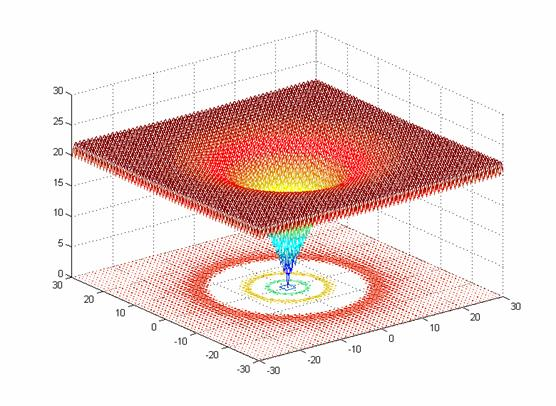
\includegraphics{image6011.jpg}
\caption{Two-dimensional Ackley function 
(\href{http://www-optima.amp.i.kyoto-u.ac.jp/member/student/hedar/Hedar\_files/TestGO\_files/Page295.htm}{image source})}\end{figure}

Public Attributes:
\begin{itemize}
\item {} 
\emph{global\_optimum} -- the problem input that produces the optimum output.
Here, this corresponds to {[}0, 0, ..., 0{]}.

\end{itemize}

\end{fulllineitems}

\index{Griewank (class in inspyred.benchmarks)}

\begin{fulllineitems}
\phantomsection\label{reference:inspyred.benchmarks.Griewank}\pysiglinewithargsret{\strong{class }\code{inspyred.benchmarks.}\bfcode{Griewank}}{\emph{dimensions=2}}{}
Defines the Griewank benchmark problem.

This class defines the Griewank global optimization problem. This 
is a highly multimodal minimization problem with numerous, wide-spread, 
regularly distributed local minima. It is defined as follows:
\begin{gather}
\begin{split}f(x) = \frac{1}{4000} \sum_{i=1}^n x_i^2 - \prod_{i=1}^n \cos(\frac{x_i}{\sqrt{i}}) + 1\end{split}\notag
\end{gather}
Here, $n$ represents the number of dimensions and $x_i \in [-600, 600]$ for $i=1,...,n$.
\begin{figure}[htbp]
\centering
\capstart

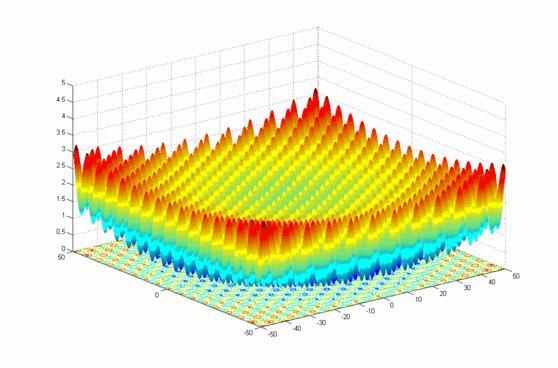
\includegraphics{image8891.jpg}
\caption{Two-dimensional Griewank function 
(\href{http://www-optima.amp.i.kyoto-u.ac.jp/member/student/hedar/Hedar\_files/TestGO\_files/Page1905.htm}{image source})}\end{figure}

Public Attributes:
\begin{itemize}
\item {} 
\emph{global\_optimum} -- the problem input that produces the optimum output.
Here, this corresponds to {[}0, 0, ..., 0{]}.

\end{itemize}

\end{fulllineitems}

\index{Rastrigin (class in inspyred.benchmarks)}

\begin{fulllineitems}
\phantomsection\label{reference:inspyred.benchmarks.Rastrigin}\pysiglinewithargsret{\strong{class }\code{inspyred.benchmarks.}\bfcode{Rastrigin}}{\emph{dimensions=2}}{}
Defines the Rastrigin benchmark problem.

This class defines the Rastrigin global optimization problem. This 
is a highly multimodal minimization problem where the local minima
are regularly distributed. It is defined as follows:
\begin{gather}
\begin{split}f(x) = \sum_{i=1}^n (x_i^2 - 10\cos(2\pi x_i) + 10)\end{split}\notag
\end{gather}
Here, $n$ represents the number of dimensions and $x_i \in [-5.12, 5.12]$ for $i=1,...,n$.
\begin{figure}[htbp]
\centering
\capstart

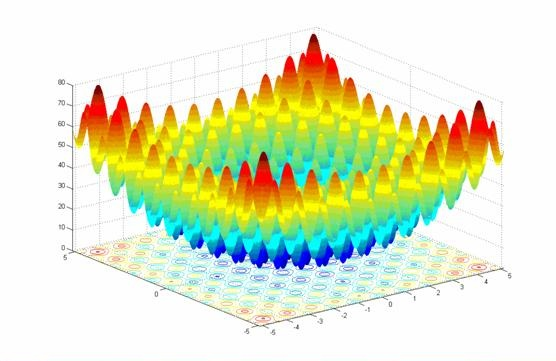
\includegraphics{image12271.jpg}
\caption{Two-dimensional Rastrigin function 
(\href{http://www-optima.amp.i.kyoto-u.ac.jp/member/student/hedar/Hedar\_files/TestGO\_files/Page2607.htm}{image source})}\end{figure}

Public Attributes:
\begin{itemize}
\item {} 
\emph{global\_optimum} -- the problem input that produces the optimum output.
Here, this corresponds to {[}0, 0, ..., 0{]}.

\end{itemize}

\end{fulllineitems}

\index{Rosenbrock (class in inspyred.benchmarks)}

\begin{fulllineitems}
\phantomsection\label{reference:inspyred.benchmarks.Rosenbrock}\pysiglinewithargsret{\strong{class }\code{inspyred.benchmarks.}\bfcode{Rosenbrock}}{\emph{dimensions=2}}{}
Defines the Rosenbrock benchmark problem.

This class defines the Rosenbrock global optimization problem, 
also known as the ``banana function.'' The global optimum sits 
within a narrow, parabolic-shaped flattened valley. It is 
defined as follows:
\begin{gather}
\begin{split}f(x) = \sum_{i=1}^{n-1} [100(x_i^2 - x_{i+1})^2 + (x_i - 1)^2]\end{split}\notag
\end{gather}
Here, $n$ represents the number of dimensions and $x_i \in [-5, 10]$ for $i=1,...,n$.
\begin{figure}[htbp]
\centering
\capstart

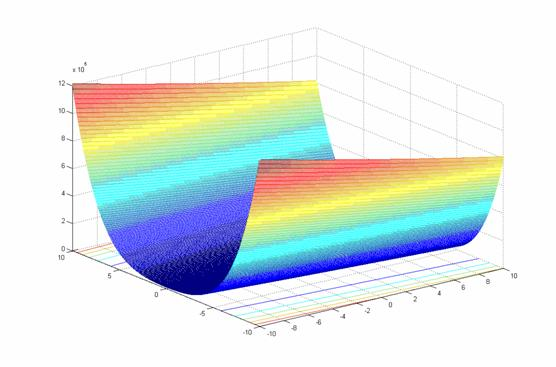
\includegraphics{image12371.jpg}
\caption{Two-dimensional Rosenbrock function 
(\href{http://www-optima.amp.i.kyoto-u.ac.jp/member/student/hedar/Hedar\_files/TestGO\_files/Page2537.htm}{image source})}\end{figure}

Public Attributes:
\begin{itemize}
\item {} 
\emph{global\_optimum} -- the problem input that produces the optimum output.
Here, this corresponds to {[}1, 1, ..., 1{]}.

\end{itemize}

\end{fulllineitems}

\index{Schwefel (class in inspyred.benchmarks)}

\begin{fulllineitems}
\phantomsection\label{reference:inspyred.benchmarks.Schwefel}\pysiglinewithargsret{\strong{class }\code{inspyred.benchmarks.}\bfcode{Schwefel}}{\emph{dimensions=2}}{}
Defines the Schwefel benchmark problem.

This class defines the Schwefel global optimization problem. 
It is defined as follows:
\begin{gather}
\begin{split}f(x) = 418.9829n - \sum_{i=1}^n \left[-x_i \sin(\sqrt{|x_i|})\right]\end{split}\notag
\end{gather}
Here, $n$ represents the number of dimensions and $x_i \in [-500, 500]$ for $i=1,...,n$.
\begin{figure}[htbp]
\centering
\capstart

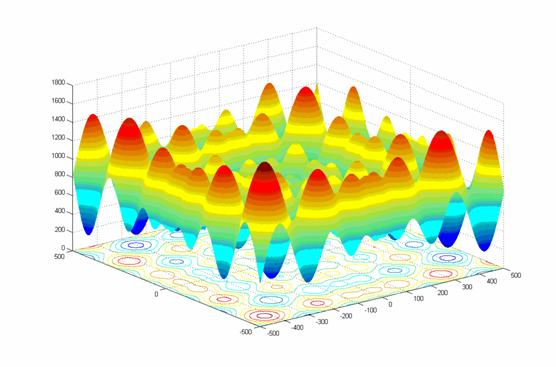
\includegraphics{image12721.jpg}
\caption{Two-dimensional Schwefel function 
(\href{http://www-optima.amp.i.kyoto-u.ac.jp/member/student/hedar/Hedar\_files/TestGO\_files/Page2530.htm}{image source})}\end{figure}

Public Attributes:
\begin{itemize}
\item {} 
\emph{global\_optimum} -- the problem input that produces the optimum output.
Here, this corresponds to {[}420.9687, 420.9687, ..., 420.9687{]}.

\end{itemize}

\end{fulllineitems}

\index{Sphere (class in inspyred.benchmarks)}

\begin{fulllineitems}
\phantomsection\label{reference:inspyred.benchmarks.Sphere}\pysiglinewithargsret{\strong{class }\code{inspyred.benchmarks.}\bfcode{Sphere}}{\emph{dimensions=2}}{}
Defines the Sphere benchmark problem.

This class defines the Sphere global optimization problem, also called
the ``first function of De Jong's'' or ``De Jong's F1.'' It is continuous,
convex, and unimodal, and it is defined as follows:
\begin{gather}
\begin{split}f(x) = \sum_{i=1}^n x_i^2\end{split}\notag
\end{gather}
Here, $n$ represents the number of dimensions and $x_i \in [-5.12, 5.12]$ for $i=1,...,n$.
\begin{figure}[htbp]
\centering
\capstart

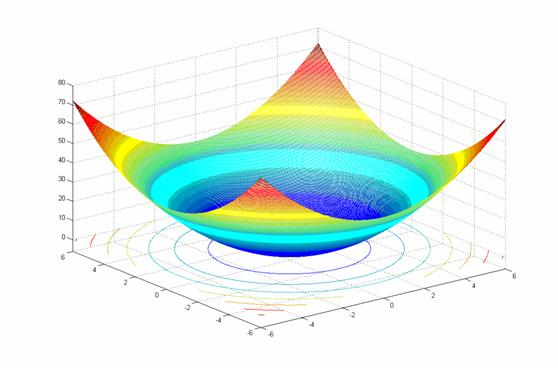
\includegraphics{image11981.jpg}
\caption{Two-dimensional Sphere function 
(\href{http://www-optima.amp.i.kyoto-u.ac.jp/member/student/hedar/Hedar\_files/TestGO\_files/Page1113.htm}{image source})}\end{figure}

Public Attributes:
\begin{itemize}
\item {} 
\emph{global\_optimum} -- the problem input that produces the optimum output.
Here, this corresponds to {[}0, 0, ..., 0{]}.

\end{itemize}

\end{fulllineitems}



\subsection{Multi-Objective Benchmarks}
\label{reference:multi-objective-benchmarks}\index{Kursawe (class in inspyred.benchmarks)}

\begin{fulllineitems}
\phantomsection\label{reference:inspyred.benchmarks.Kursawe}\pysiglinewithargsret{\strong{class }\code{inspyred.benchmarks.}\bfcode{Kursawe}}{\emph{dimensions=2}}{}
Defines the Kursawe multiobjective benchmark problem.

This class defines the Kursawe multiobjective minimization problem. 
This function accepts an n-dimensional input and produces a 
two-dimensional output. It is defined as follows:
\begin{gather}
\begin{split}f_1(x) &= \sum_{i=1}^{n-1} \left[-10e^{-0.2\sqrt{x_i^2 + x_{i+1}^2}}\right] \\
f_2(x) &= \sum_{i=1}^n \left[|x_i|^{0.8} + 5\sin(x_i)^3\right] \\\end{split}\notag
\end{gather}
Here, $n$ represents the number of dimensions and $x_i \in [-5, 5]$ for $i=1,...,n$.
\begin{figure}[htbp]
\centering
\capstart

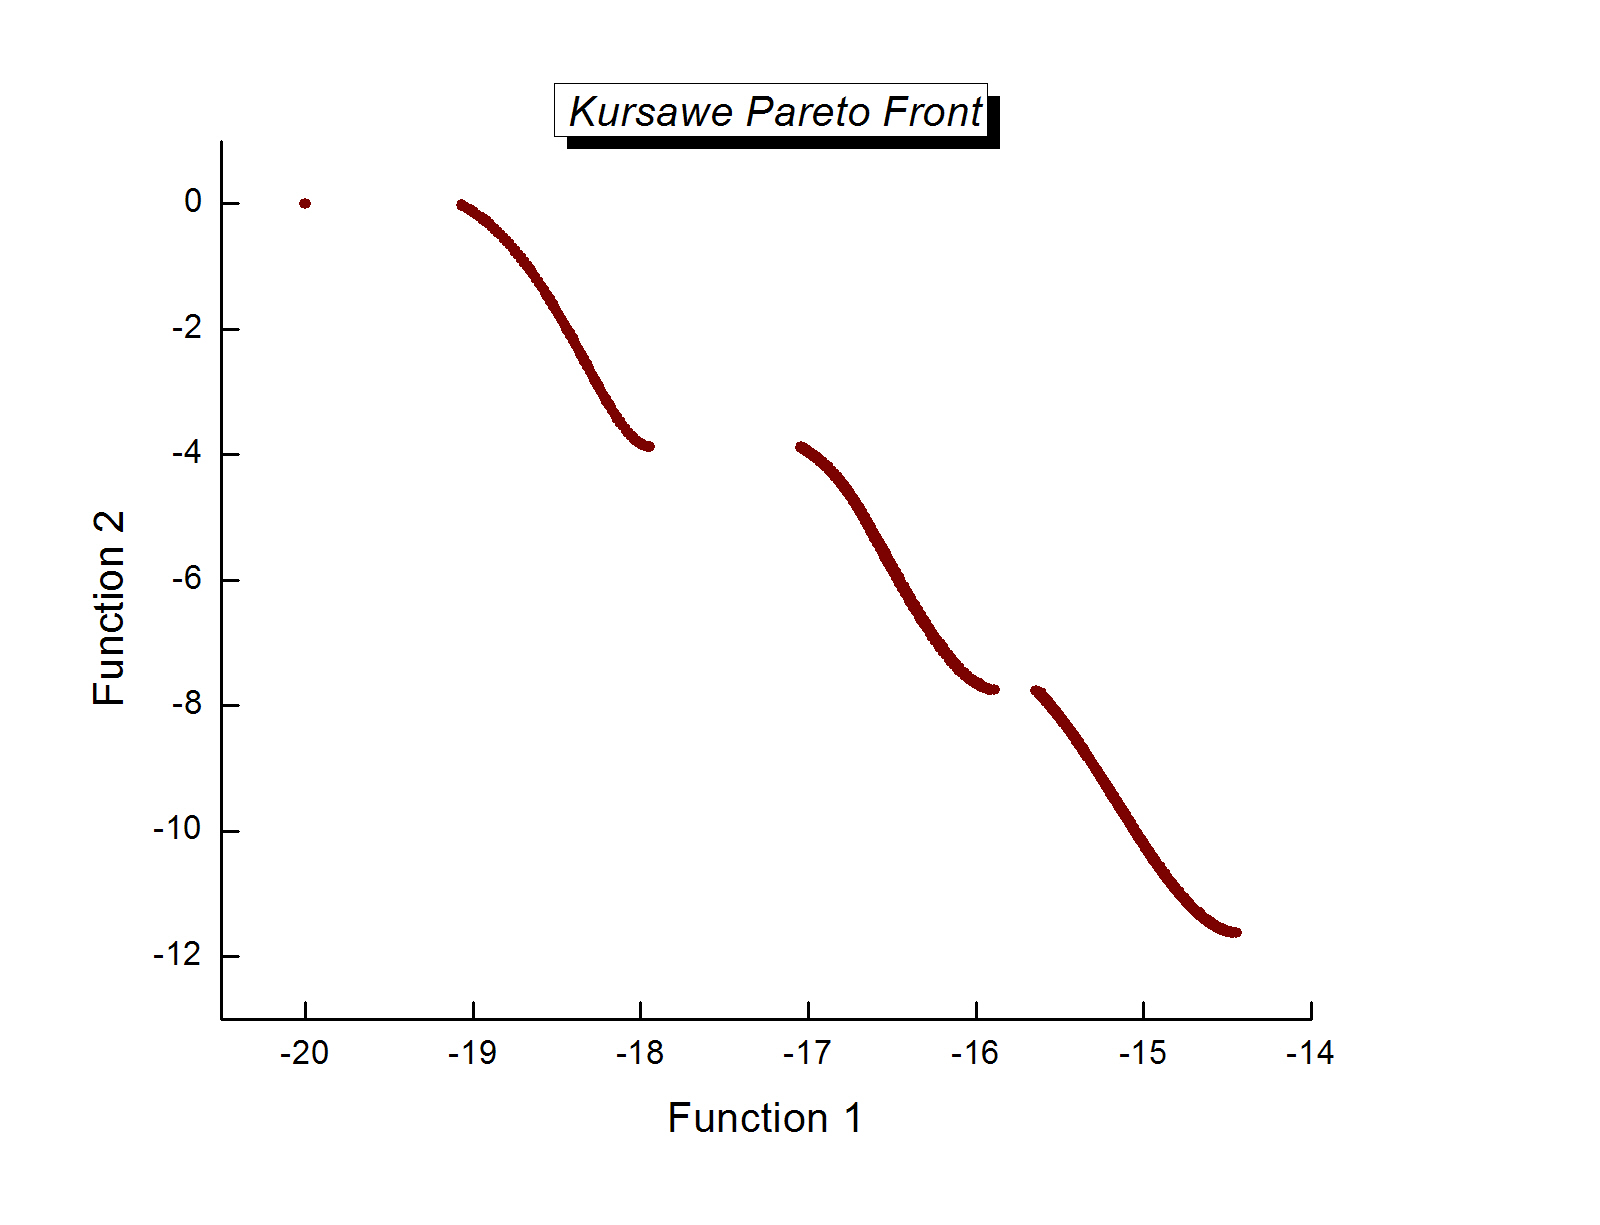
\includegraphics{kursawefun.jpg}
\caption{Three-dimensional Kursawe Pareto front 
(\href{http://delta.cs.cinvestav.mx/~ccoello/EMOO/testfuncs/}{image source})}\end{figure}

\end{fulllineitems}

\index{DTLZ1 (class in inspyred.benchmarks)}

\begin{fulllineitems}
\phantomsection\label{reference:inspyred.benchmarks.DTLZ1}\pysiglinewithargsret{\strong{class }\code{inspyred.benchmarks.}\bfcode{DTLZ1}}{\emph{dimensions=2}, \emph{objectives=2}}{}
Defines the DTLZ1 multiobjective benchmark problem.

This class defines the DTLZ1 multiobjective minimization problem
taken from \href{http://www.tik.ee.ethz.ch/sop/download/supplementary/testproblems/dtlz1/index.php}{(Deb et al., ``Scalable Multi-Objective Optimization Test Problems.''
CEC 2002, pp. 825--830)}.
This function accepts an n-dimensional input and produces an m-dimensional output.
It is defined as follows:
\begin{gather}
\begin{split}f_1(\vec{x}) &= \frac{1}{2} x_1 \dots x_{m-1}(1 + g(\vec{x_m})) \\
f_i(\vec{x}) &= \frac{1}{2} x_1 \dots x_{m-i}(1 + g(\vec{x_m})) \\
f_m(\vec{x}) &= \frac{1}{2} (1 - x_1)(1 + g(\vec{x_m})) \\
g(\vec{x_m}) &= 100\left[|\vec{x_m}| + \sum_{x_i \in \vec{x_m}}\left((x_i - 0.5)^2 - \cos(20\pi(x_i - 0.5))\right)\right] \\\end{split}\notag
\end{gather}
Here, $n$ represents the number of dimensions, $m$ represents the
number of objectives, $x_i \in [0, 1]$ for $i=1,...,n$, and 
$\vec{x_m} = x_m x_{m+1} \dots x_{n}.$

The recommendation given in the paper mentioned above is to provide 4 more
dimensions than objectives. For instance, if we want to use 2 objectives, we
should use 6 dimensions.
\begin{figure}[htbp]
\centering
\capstart

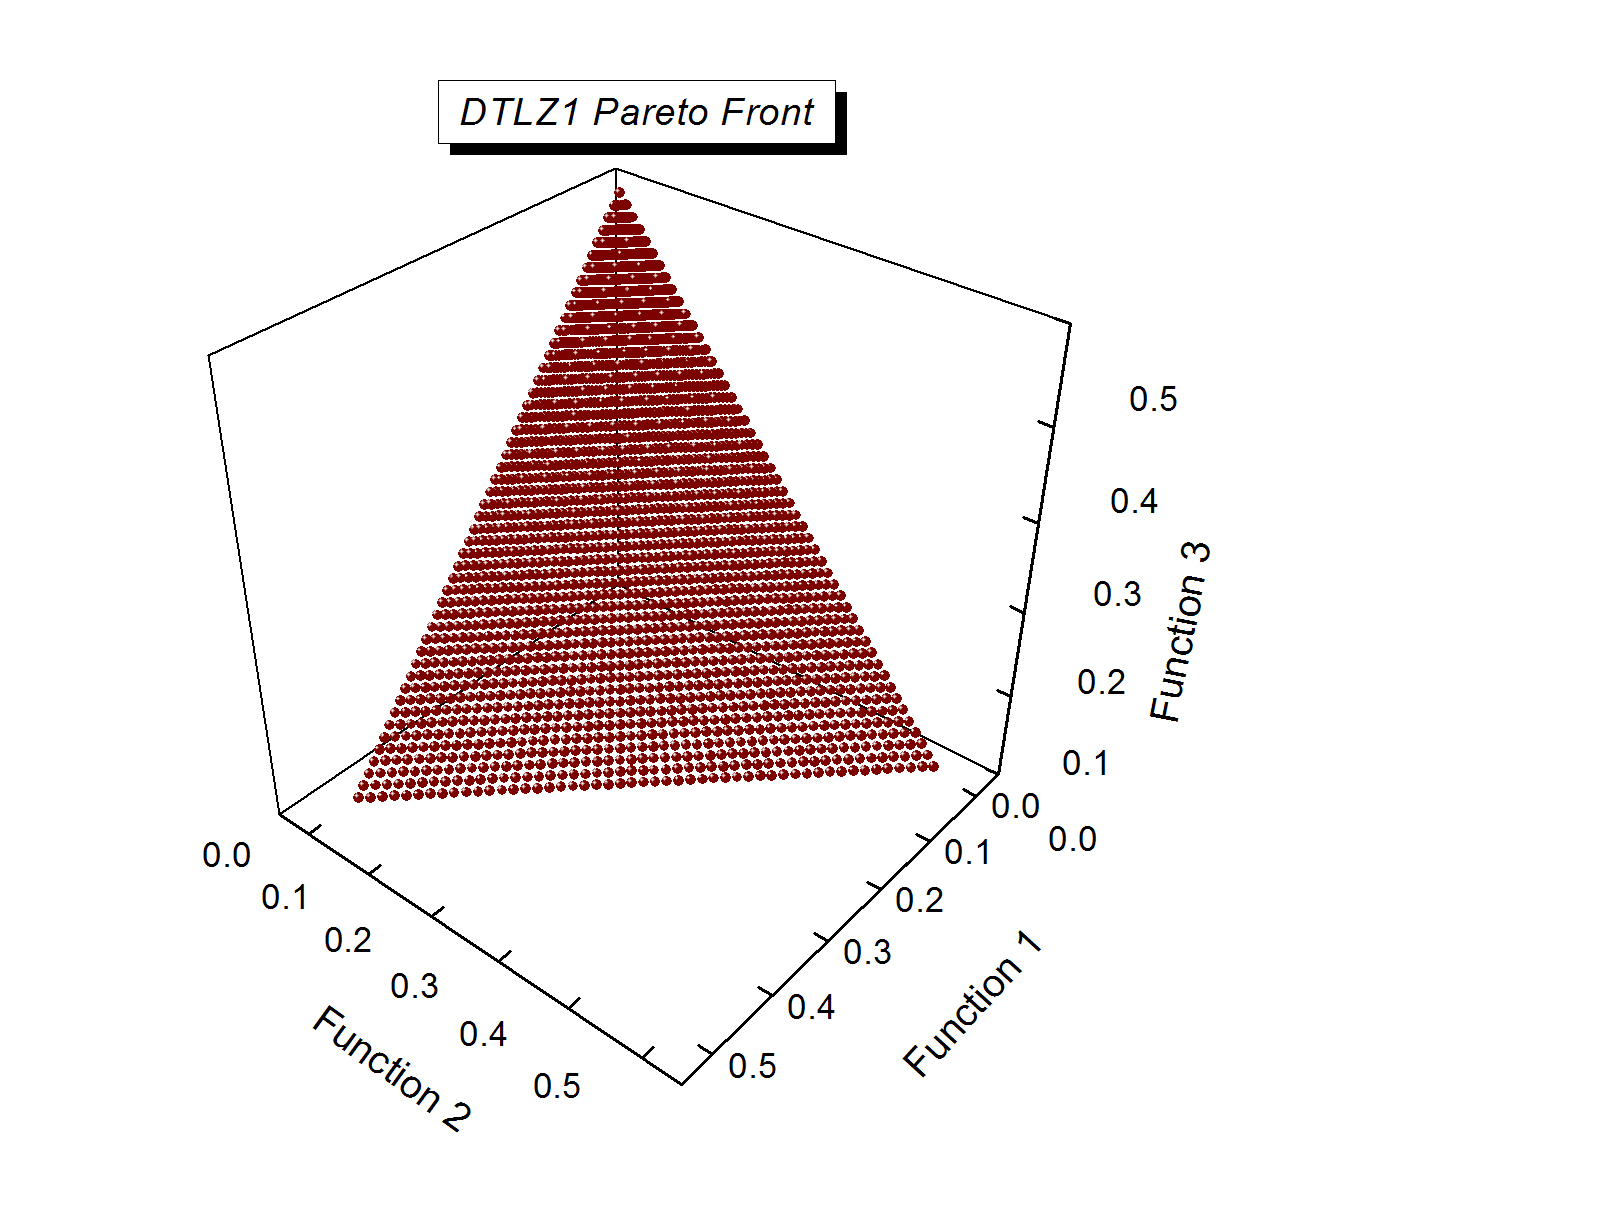
\includegraphics{dtlz1funb.jpg}
\caption{Three-dimensional DTLZ1 Pareto front 
(\href{http://delta.cs.cinvestav.mx/~ccoello/EMOO/testfuncs/}{image source})}\end{figure}
\index{global\_optimum() (inspyred.benchmarks.DTLZ1 method)}

\begin{fulllineitems}
\phantomsection\label{reference:inspyred.benchmarks.DTLZ1.global_optimum}\pysiglinewithargsret{\bfcode{global\_optimum}}{}{}
Return a globally optimal solution to this problem.

This function returns a globally optimal solution (i.e., a 
solution that lives on the Pareto front). Since there are many
solutions that are Pareto-optimal, this function randomly 
chooses one to return.

\end{fulllineitems}


\end{fulllineitems}

\index{DTLZ2 (class in inspyred.benchmarks)}

\begin{fulllineitems}
\phantomsection\label{reference:inspyred.benchmarks.DTLZ2}\pysiglinewithargsret{\strong{class }\code{inspyred.benchmarks.}\bfcode{DTLZ2}}{\emph{dimensions=2}, \emph{objectives=2}}{}
Defines the DTLZ2 multiobjective benchmark problem.

This class defines the DTLZ2 multiobjective minimization problem
taken from \href{http://www.tik.ee.ethz.ch/sop/download/supplementary/testproblems/dtlz1/index.php}{(Deb et al., ``Scalable Multi-Objective Optimization Test Problems.''
CEC 2002, pp. 825--830)}.
This function accepts an n-dimensional input and produces an m-dimensional output.
It is defined as follows:
\begin{gather}
\begin{split}f_1(\vec{x}) &= (1 + g(\vec{x_m}))\cos(x_1 \pi/2)\cos(x_2 \pi/2)\dots\cos(x_{m-2} \pi/2)\cos(x_{m-1} \pi/2) \\
f_i(\vec{x}) &= (1 + g(\vec{x_m}))\cos(x_1 \pi/2)\cos(x_2 \pi/2)\dots\cos(x_{m-i} \pi/2)\sin(x_{m-i+1} \pi/2) \\
f_m(\vec{x}) &= (1 + g(\vec{x_m}))\sin(x_1 \pi/2) \\
g(\vec{x_m}) &= \sum_{x_i \in \vec{x_m}}(x_i - 0.5)^2 \\\end{split}\notag
\end{gather}
Here, $n$ represents the number of dimensions, $m$ represents the
number of objectives, $x_i \in [0, 1]$ for $i=1,...,n$, and 
$\vec{x_m} = x_m x_{m+1} \dots x_{n}.$

The recommendation given in the paper mentioned above is to provide 9 more
dimensions than objectives. For instance, if we want to use 2 objectives, we
should use 11 dimensions.
\index{global\_optimum() (inspyred.benchmarks.DTLZ2 method)}

\begin{fulllineitems}
\phantomsection\label{reference:inspyred.benchmarks.DTLZ2.global_optimum}\pysiglinewithargsret{\bfcode{global\_optimum}}{}{}
Return a globally optimal solution to this problem.

This function returns a globally optimal solution (i.e., a 
solution that lives on the Pareto front). Since there are many
solutions that are Pareto-optimal, this function randomly 
chooses one to return.

\end{fulllineitems}


\end{fulllineitems}

\index{DTLZ3 (class in inspyred.benchmarks)}

\begin{fulllineitems}
\phantomsection\label{reference:inspyred.benchmarks.DTLZ3}\pysiglinewithargsret{\strong{class }\code{inspyred.benchmarks.}\bfcode{DTLZ3}}{\emph{dimensions=2}, \emph{objectives=2}}{}
Defines the DTLZ3 multiobjective benchmark problem.

This class defines the DTLZ3 multiobjective minimization problem
taken from \href{http://www.tik.ee.ethz.ch/sop/download/supplementary/testproblems/dtlz1/index.php}{(Deb et al., ``Scalable Multi-Objective Optimization Test Problems.''
CEC 2002, pp. 825--830)}.
This function accepts an n-dimensional input and produces an m-dimensional output.
It is defined as follows:
\begin{gather}
\begin{split}f_1(\vec{x}) &= (1 + g(\vec{x_m}))\cos(x_1 \pi/2)\cos(x_2 \pi/2)\dots\cos(x_{m-2} \pi/2)\cos(x_{m-1} \pi/2) \\
f_i(\vec{x}) &= (1 + g(\vec{x_m}))\cos(x_1 \pi/2)\cos(x_2 \pi/2)\dots\cos(x_{m-i} \pi/2)\sin(x_{m-i+1} \pi/2) \\
f_m(\vec{x}) &= (1 + g(\vec{x_m}))\sin(x_1 \pi/2) \\
g(\vec{x_m}) &= 100\left[|\vec{x_m}| + \sum_{x_i \in \vec{x_m}}\left((x_i - 0.5)^2 - \cos(20\pi(x_i - 0.5))\right)\right] \\\end{split}\notag
\end{gather}
Here, $n$ represents the number of dimensions, $m$ represents the
number of objectives, $x_i \in [0, 1]$ for $i=1,...,n$, and 
$\vec{x_m} = x_m x_{m+1} \dots x_{n}.$

The recommendation given in the paper mentioned above is to provide 9 more
dimensions than objectives. For instance, if we want to use 2 objectives, we
should use 11 dimensions.
\index{global\_optimum() (inspyred.benchmarks.DTLZ3 method)}

\begin{fulllineitems}
\phantomsection\label{reference:inspyred.benchmarks.DTLZ3.global_optimum}\pysiglinewithargsret{\bfcode{global\_optimum}}{}{}
Return a globally optimal solution to this problem.

This function returns a globally optimal solution (i.e., a 
solution that lives on the Pareto front). Since there are many
solutions that are Pareto-optimal, this function randomly 
chooses one to return.

\end{fulllineitems}


\end{fulllineitems}

\index{DTLZ4 (class in inspyred.benchmarks)}

\begin{fulllineitems}
\phantomsection\label{reference:inspyred.benchmarks.DTLZ4}\pysiglinewithargsret{\strong{class }\code{inspyred.benchmarks.}\bfcode{DTLZ4}}{\emph{dimensions=2}, \emph{objectives=2}, \emph{alpha=100}}{}
Defines the DTLZ4 multiobjective benchmark problem.

This class defines the DTLZ4 multiobjective minimization problem
taken from \href{http://www.tik.ee.ethz.ch/sop/download/supplementary/testproblems/dtlz1/index.php}{(Deb et al., ``Scalable Multi-Objective Optimization Test Problems.''
CEC 2002, pp. 825--830)}.
This function accepts an n-dimensional input and produces an m-dimensional output.
It is defined as follows:
\begin{gather}
\begin{split}f_1(\vec{x}) &= (1 + g(\vec{x_m}))\cos(x_1^\alpha \pi/2)\cos(x_2^\alpha \pi/2)\dots\cos(x_{m-2}^\alpha \pi/2)\cos(x_{m-1}^\alpha \pi/2) \\
f_i(\vec{x}) &= (1 + g(\vec{x_m}))\cos(x_1^\alpha \pi/2)\cos(x_2^\alpha \pi/2)\dots\cos(x_{m-i}^\alpha \pi/2)\sin(x_{m-i+1}^\alpha \pi/2) \\
f_m(\vec{x}) &= (1 + g(\vec{x_m}))\sin(x_1^\alpha \pi/2) \\
g(\vec{x_m}) &= \sum_{x_i \in \vec{x_m}}(x_i - 0.5)^2 \\\end{split}\notag
\end{gather}
Here, $n$ represents the number of dimensions, $m$ represents the
number of objectives, $x_i \in [0, 1]$ for $i=1,...,n$,  
$\vec{x_m} = x_m x_{m+1} \dots x_{n},$ and $\alpha=100.$

The recommendation given in the paper mentioned above is to provide 9 more
dimensions than objectives. For instance, if we want to use 2 objectives, we
should use 11 dimensions.
\index{global\_optimum() (inspyred.benchmarks.DTLZ4 method)}

\begin{fulllineitems}
\phantomsection\label{reference:inspyred.benchmarks.DTLZ4.global_optimum}\pysiglinewithargsret{\bfcode{global\_optimum}}{}{}
Return a globally optimal solution to this problem.

This function returns a globally optimal solution (i.e., a 
solution that lives on the Pareto front). Since there are many
solutions that are Pareto-optimal, this function randomly 
chooses one to return.

\end{fulllineitems}


\end{fulllineitems}

\index{DTLZ5 (class in inspyred.benchmarks)}

\begin{fulllineitems}
\phantomsection\label{reference:inspyred.benchmarks.DTLZ5}\pysiglinewithargsret{\strong{class }\code{inspyred.benchmarks.}\bfcode{DTLZ5}}{\emph{dimensions=2}, \emph{objectives=2}}{}
Defines the DTLZ5 multiobjective benchmark problem.

This class defines the DTLZ5 multiobjective minimization problem
taken from \href{http://www.tik.ee.ethz.ch/sop/download/supplementary/testproblems/dtlz1/index.php}{(Deb et al., ``Scalable Multi-Objective Optimization Test Problems.''
CEC 2002, pp. 825--830)}.
This function accepts an n-dimensional input and produces an m-dimensional output.
It is defined as follows:
\begin{gather}
\begin{split}f_1(\vec{x}) &= (1 + g(\vec{x_m}))\cos(\theta_1 \pi/2)\cos(\theta_2 \pi/2)\dots\cos(\theta_{m-2} \pi/2)\cos(\theta_{m-1} \pi/2) \\
f_i(\vec{x}) &= (1 + g(\vec{x_m}))\cos(\theta_1 \pi/2)\cos(\theta_2 \pi/2)\dots\cos(\theta_{m-i} \pi/2)\sin(\theta_{m-i+1} \pi/2) \\
f_m(\vec{x}) &= (1 + g(\vec{x_m}))\sin(\theta_1 \pi/2) \\
\theta_i     &= \frac{\pi}{4(1+g(\vec{x_m}))}(1 + 2g(\vec{x_m}) x_i) \\
g(\vec{x_m}) &= \sum_{x_i \in \vec{x_m}}(x_i - 0.5)^2 \\\end{split}\notag
\end{gather}
Here, $n$ represents the number of dimensions, $m$ represents the
number of objectives, $x_i \in [0, 1]$ for $i=1,...,n$, and 
$\vec{x_m} = x_m x_{m+1} \dots x_{n}.$

The recommendation given in the paper mentioned above is to provide 9 more
dimensions than objectives. For instance, if we want to use 2 objectives, we
should use 11 dimensions.
\index{global\_optimum() (inspyred.benchmarks.DTLZ5 method)}

\begin{fulllineitems}
\phantomsection\label{reference:inspyred.benchmarks.DTLZ5.global_optimum}\pysiglinewithargsret{\bfcode{global\_optimum}}{}{}
Return a globally optimal solution to this problem.

This function returns a globally optimal solution (i.e., a 
solution that lives on the Pareto front). Since there are many
solutions that are Pareto-optimal, this function randomly 
chooses one to return.

\end{fulllineitems}


\end{fulllineitems}

\index{DTLZ6 (class in inspyred.benchmarks)}

\begin{fulllineitems}
\phantomsection\label{reference:inspyred.benchmarks.DTLZ6}\pysiglinewithargsret{\strong{class }\code{inspyred.benchmarks.}\bfcode{DTLZ6}}{\emph{dimensions=2}, \emph{objectives=2}}{}
Defines the DTLZ6 multiobjective benchmark problem.

This class defines the DTLZ6 multiobjective minimization problem
taken from \href{http://www.tik.ee.ethz.ch/sop/download/supplementary/testproblems/dtlz1/index.php}{(Deb et al., ``Scalable Multi-Objective Optimization Test Problems.''
CEC 2002, pp. 825--830)}.
This function accepts an n-dimensional input and produces an m-dimensional output.
It is defined as follows:
\begin{gather}
\begin{split}f_1(\vec{x}) &= (1 + g(\vec{x_m}))\cos(\theta_1 \pi/2)\cos(\theta_2 \pi/2)\dots\cos(\theta_{m-2} \pi/2)\cos(\theta_{m-1} \pi/2) \\
f_i(\vec{x}) &= (1 + g(\vec{x_m}))\cos(\theta_1 \pi/2)\cos(\theta_2 \pi/2)\dots\cos(\theta_{m-i} \pi/2)\sin(\theta_{m-i+1} \pi/2) \\
f_m(\vec{x}) &= (1 + g(\vec{x_m}))\sin(\theta_1 \pi/2) \\
\theta_i     &= \frac{\pi}{4(1+g(\vec{x_m}))}(1 + 2g(\vec{x_m}) x_i) \\
g(\vec{x_m}) &= \sum_{x_i \in \vec{x_m}}x_i^{0.1} \\\end{split}\notag
\end{gather}
Here, $n$ represents the number of dimensions, $m$ represents the
number of objectives, $x_i \in [0, 1]$ for $i=1,...,n$, and 
$\vec{x_m} = x_m x_{m+1} \dots x_{n}.$

The recommendation given in the paper mentioned above is to provide 9 more
dimensions than objectives. For instance, if we want to use 2 objectives, we
should use 11 dimensions.
\index{global\_optimum() (inspyred.benchmarks.DTLZ6 method)}

\begin{fulllineitems}
\phantomsection\label{reference:inspyred.benchmarks.DTLZ6.global_optimum}\pysiglinewithargsret{\bfcode{global\_optimum}}{}{}
Return a globally optimal solution to this problem.

This function returns a globally optimal solution (i.e., a 
solution that lives on the Pareto front). Since there are many
solutions that are Pareto-optimal, this function randomly 
chooses one to return.

\end{fulllineitems}


\end{fulllineitems}

\index{DTLZ7 (class in inspyred.benchmarks)}

\begin{fulllineitems}
\phantomsection\label{reference:inspyred.benchmarks.DTLZ7}\pysiglinewithargsret{\strong{class }\code{inspyred.benchmarks.}\bfcode{DTLZ7}}{\emph{dimensions=2}, \emph{objectives=2}}{}
Defines the DTLZ7 multiobjective benchmark problem.

This class defines the DTLZ7 multiobjective minimization problem
taken from \href{http://www.tik.ee.ethz.ch/sop/download/supplementary/testproblems/dtlz1/index.php}{(Deb et al., ``Scalable Multi-Objective Optimization Test Problems.''
CEC 2002, pp. 825--830)}.
This function accepts an n-dimensional input and produces an m-dimensional output.
It is defined as follows:
\begin{gather}
\begin{split}f_1(\vec{x}) &= x_1 \\
f_i(\vec{x}) &= x_i \\
f_m(\vec{x}) &= (1 + g(\vec{x_m}))h(f_1, f_2, \dots, f_{m-1}, g) \\
g(\vec{x_m}) &= 1 + \frac{9}{|\vec{x_m}|}\sum_{x_i \in \vec{x_m}}x_i \\
h(f_1, f_2, \dots, f_{m-1}, g) &= m - \sum_{i=1}^{m-1}\left[\frac{f_1}{1+g}(1 + \sin(3\pi f_i))\right] \\\end{split}\notag
\end{gather}
Here, $n$ represents the number of dimensions, $m$ represents the
number of objectives, $x_i \in [0, 1]$ for $i=1,...,n$, and 
$\vec{x_m} = x_m x_{m+1} \dots x_{n}.$

The recommendation given in the paper mentioned above is to provide 19 more
dimensions than objectives. For instance, if we want to use 2 objectives, we
should use 21 dimensions.
\begin{figure}[htbp]
\centering
\capstart

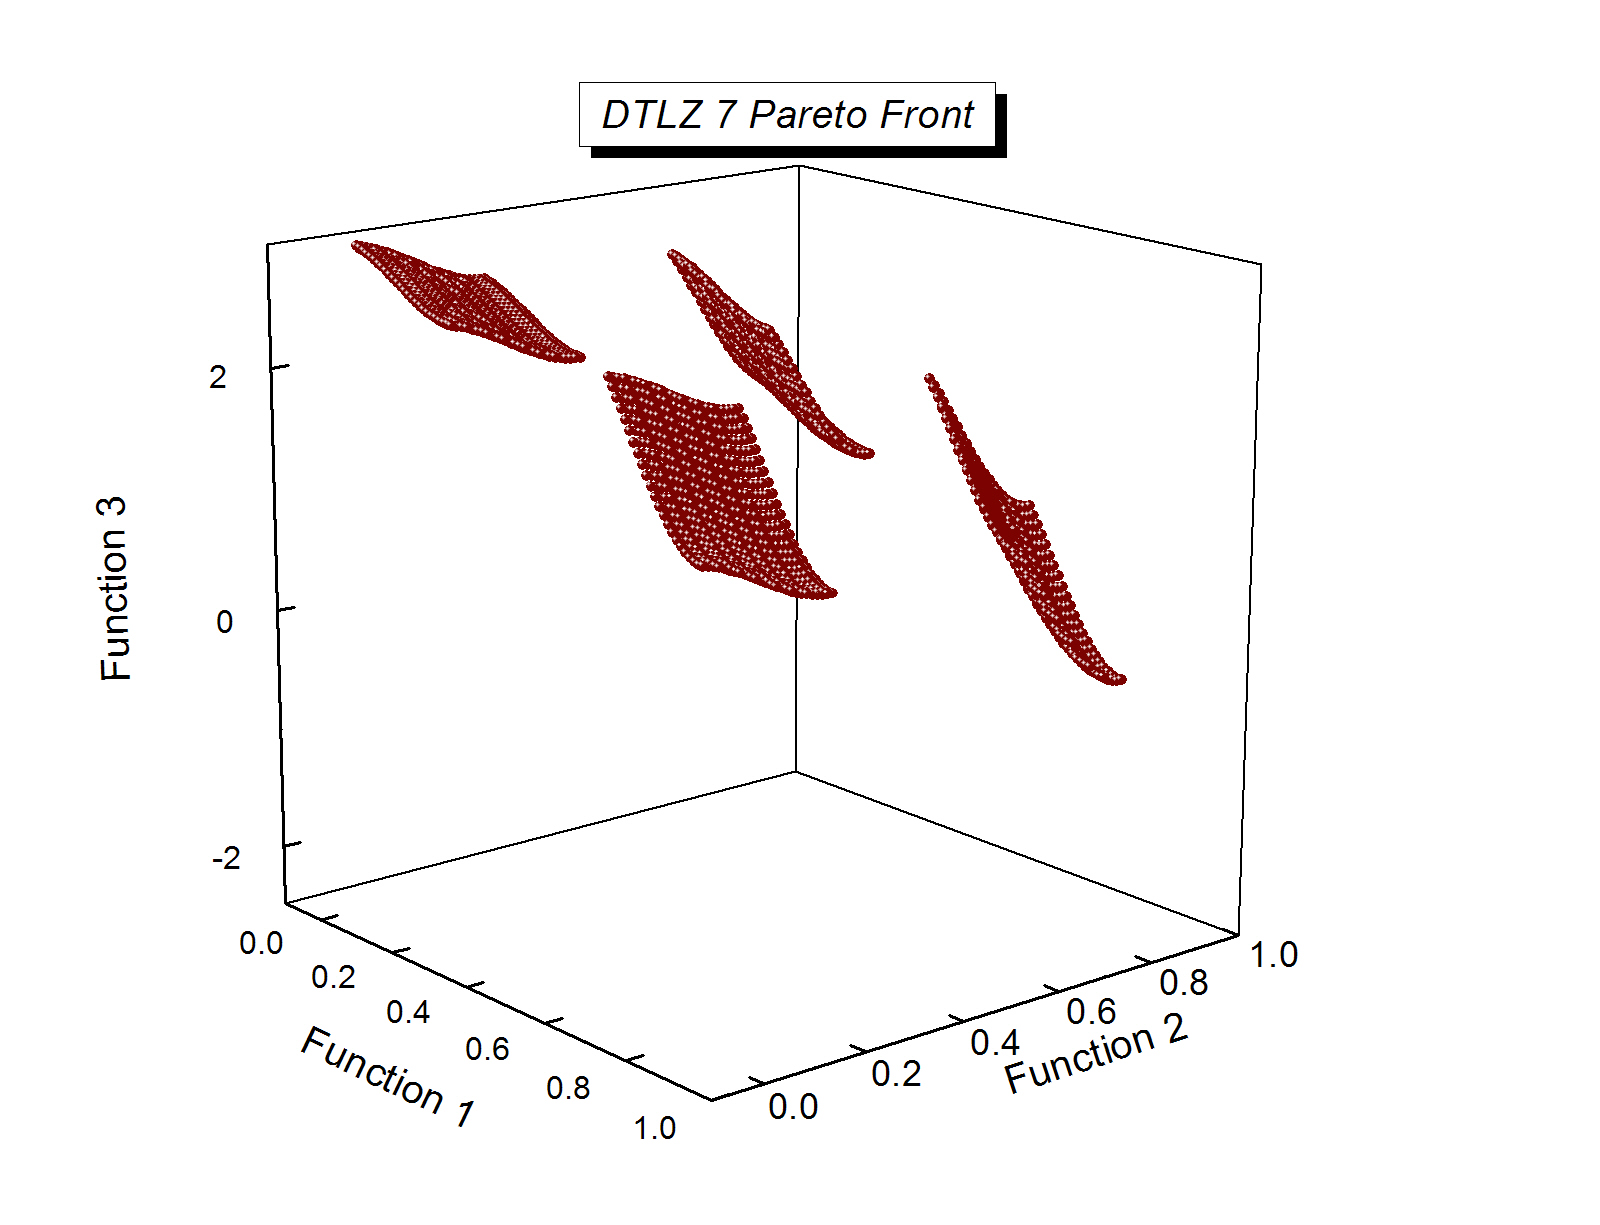
\includegraphics{dtlz7funb.jpg}
\caption{Three-dimensional DTLZ7 Pareto front 
(\href{http://delta.cs.cinvestav.mx/~ccoello/EMOO/testfuncs/}{image source})}\end{figure}
\index{global\_optimum() (inspyred.benchmarks.DTLZ7 method)}

\begin{fulllineitems}
\phantomsection\label{reference:inspyred.benchmarks.DTLZ7.global_optimum}\pysiglinewithargsret{\bfcode{global\_optimum}}{}{}
Return a globally optimal solution to this problem.

This function returns a globally optimal solution (i.e., a 
solution that lives on the Pareto front). Since there are many
solutions that are Pareto-optimal, this function randomly 
chooses one to return.

\end{fulllineitems}


\end{fulllineitems}



\subsection{Discrete Optimization Benchmarks}
\label{reference:discrete-optimization-benchmarks}\index{Knapsack (class in inspyred.benchmarks)}

\begin{fulllineitems}
\phantomsection\label{reference:inspyred.benchmarks.Knapsack}\pysiglinewithargsret{\strong{class }\code{inspyred.benchmarks.}\bfcode{Knapsack}}{\emph{capacity}, \emph{items}, \emph{duplicates=False}}{}
Defines the Knapsack benchmark problem.

This class defines the Knapsack problem: given a set of items, each
with a weight and a value, find the set of items of maximal value
that fit within a knapsack of fixed weight capacity. This problem 
assumes that the \code{items} parameter is a list of (weight, value) 
tuples. This problem is most easily defined as a maximization problem,
where the total value contained in the knapsack is to be maximized.
However, for the evolutionary computation (which may create infeasible
solutions that exceed the knapsack capacity), the fitness is either
the total value in the knapsack (for feasible solutions) or the
negative difference between the actual contents and the maximum 
capacity of the knapsack.

If evolutionary computation is to be used, then the \code{generator} 
function should be used to create candidates. If ant colony 
optimization is used, then the \code{constructor} function creates 
candidates. The \code{evaluator} function performs the evaluation for 
both types of candidates.

Public Attributes:
\begin{itemize}
\item {} 
\emph{capacity} -- the weight capacity of the knapsack

\item {} 
\emph{items} -- a list of (weight, value) tuples corresponding to the
possible items to be placed into the knapsack

\item {} 
\emph{components} -- the set of \code{TrailComponent} objects constructed
from the \code{items} parameter

\item {} 
\emph{duplicates} -- Boolean value specifying whether items may be 
duplicated in the knapsack (i.e., False corresponds to 0/1 Knapsack)

\item {} 
\emph{bias} -- the bias in selecting the component of maximum desirability
when constructing a candidate solution for ant colony optimization 
(default 0.5)

\end{itemize}
\index{constructor() (inspyred.benchmarks.Knapsack method)}

\begin{fulllineitems}
\phantomsection\label{reference:inspyred.benchmarks.Knapsack.constructor}\pysiglinewithargsret{\bfcode{constructor}}{\emph{random}, \emph{args}}{}
Return a candidate solution for an ant colony optimization.

\end{fulllineitems}

\index{evaluator() (inspyred.benchmarks.Knapsack method)}

\begin{fulllineitems}
\phantomsection\label{reference:inspyred.benchmarks.Knapsack.evaluator}\pysiglinewithargsret{\bfcode{evaluator}}{\emph{candidates}, \emph{args}}{}
Return the fitness values for the given candidates.

\end{fulllineitems}

\index{generator() (inspyred.benchmarks.Knapsack method)}

\begin{fulllineitems}
\phantomsection\label{reference:inspyred.benchmarks.Knapsack.generator}\pysiglinewithargsret{\bfcode{generator}}{\emph{random}, \emph{args}}{}
Return a candidate solution for an evolutionary computation.

\end{fulllineitems}


\end{fulllineitems}

\index{TSP (class in inspyred.benchmarks)}

\begin{fulllineitems}
\phantomsection\label{reference:inspyred.benchmarks.TSP}\pysiglinewithargsret{\strong{class }\code{inspyred.benchmarks.}\bfcode{TSP}}{\emph{weights}}{}
Defines the Traveling Salesman benchmark problem.

This class defines the Traveling Salesman problem: given a set of
locations and their pairwise distances, find the shortest route that
visits each location once and only once. This problem assumes that 
the \code{weights} parameter is an \emph{n}-by-\emph{n} list of pairwise 
distances among \emph{n} locations. This problem is treated as a 
maximization problem, so fitness values are determined to be the 
reciprocal of the total path length.

In the case of typical evolutionary computation, a candidate solution
is represented as a permutation of the \emph{n}-element list of the integers 
from 0 to \emph{n}-1. In the case of ant colony optimization, a candidate
solution is represented by a list of \code{TrailComponent} objects which
have (source, destination) tuples as their elements and the reciprocal
of the weight from source to destination as their values.

If evolutionary computation is to be used, then the \code{generator} 
function should be used to create candidates. If ant colony 
optimization is used, then the \code{constructor} function creates 
candidates. The \code{evaluator} function performs the evaluation for 
both types of candidates.

Public Attributes:
\begin{itemize}
\item {} 
\emph{weights} -- the two-dimensional list of pairwise distances

\item {} 
\emph{components} -- the set of \code{TrailComponent} objects constructed
from the \code{weights} attribute, where the element is the (source,
destination) tuple and the value is the reciprocal of its 
\code{weights} entry

\item {} 
\emph{bias} -- the bias in selecting the component of maximum desirability
when constructing a candidate solution for ant colony optimization 
(default 0.5)

\end{itemize}
\index{constructor() (inspyred.benchmarks.TSP method)}

\begin{fulllineitems}
\phantomsection\label{reference:inspyred.benchmarks.TSP.constructor}\pysiglinewithargsret{\bfcode{constructor}}{\emph{random}, \emph{args}}{}
Return a candidate solution for an ant colony optimization.

\end{fulllineitems}

\index{evaluator() (inspyred.benchmarks.TSP method)}

\begin{fulllineitems}
\phantomsection\label{reference:inspyred.benchmarks.TSP.evaluator}\pysiglinewithargsret{\bfcode{evaluator}}{\emph{candidates}, \emph{args}}{}
Return the fitness values for the given candidates.

\end{fulllineitems}

\index{generator() (inspyred.benchmarks.TSP method)}

\begin{fulllineitems}
\phantomsection\label{reference:inspyred.benchmarks.TSP.generator}\pysiglinewithargsret{\bfcode{generator}}{\emph{random}, \emph{args}}{}
Return a candidate solution for an evolutionary computation.

\end{fulllineitems}


\end{fulllineitems}



\chapter{Troubleshooting}
\label{troubleshooting::doc}\label{troubleshooting:troubleshooting}
Given the flexibility of the inspyred library, along with the inherent stochasticity of the algorithms, it can be difficult to track down errors that will inevitably arise. This chapter provides some suggestions that may make the process easier.


\section{Always Store the Seed}
\label{troubleshooting:always-store-the-seed}
Every inspyred algorithm requires that a pseudo-random number generator (PRNG) object be passed to it. This allows users to make use of different PRNGs if more sophisticated random number generation is desired (as long as it implements the relevant methods of Python's \code{Random} class). This also means that the PRNG must be seeded prior to its passing to an inspyred algorithm. This seed should always be printed (preferably to a file) in case the exact run of the algorithm needs to be duplicated. If an error occurs in a given run, it can be restarted by providing the same seed. The following code provides an example:

\begin{Verbatim}[commandchars=\\\{\}]
\PYG{k+kn}{import} \PYG{n+nn}{random}
\PYG{k+kn}{import} \PYG{n+nn}{time}
\PYG{n}{my\PYGZus{}seed} \PYG{o}{=} \PYG{n+nb}{int}\PYG{p}{(}\PYG{n}{time}\PYG{o}{.}\PYG{n}{time}\PYG{p}{(}\PYG{p}{)}\PYG{p}{)}
\PYG{n}{seedfile} \PYG{o}{=} \PYG{n+nb}{open}\PYG{p}{(}\PYG{l+s}{'}\PYG{l+s}{randomseed.txt}\PYG{l+s}{'}\PYG{p}{,} \PYG{l+s}{'}\PYG{l+s}{w}\PYG{l+s}{'}\PYG{p}{)}
\PYG{n}{seedfile}\PYG{o}{.}\PYG{n}{write}\PYG{p}{(}\PYG{l+s}{'}\PYG{l+s}{\PYGZob{}0\PYGZcb{}}\PYG{l+s}{'}\PYG{o}{.}\PYG{n}{format}\PYG{p}{(}\PYG{n}{my\PYGZus{}seed}\PYG{p}{)}\PYG{p}{)}
\PYG{n}{seedfile}\PYG{o}{.}\PYG{n}{close}\PYG{p}{(}\PYG{p}{)}
\PYG{n}{prng} \PYG{o}{=} \PYG{n}{random}\PYG{o}{.}\PYG{n}{Random}\PYG{p}{(}\PYG{p}{)}
\PYG{n}{prng}\PYG{o}{.}\PYG{n}{seed}\PYG{p}{(}\PYG{n}{my\PYGZus{}seed}\PYG{p}{)}
\end{Verbatim}


\section{Use and Consult the Logs}
\label{troubleshooting:use-and-consult-the-logs}
All inspyred algorithms provide detailed debugging data using Python's core \code{logging} module. This can be enabled by adding the following code to the \code{main} or calling scope:

\begin{Verbatim}[commandchars=\\\{\}]
\PYG{k+kn}{import} \PYG{n+nn}{logging}
\PYG{n}{logger} \PYG{o}{=} \PYG{n}{logging}\PYG{o}{.}\PYG{n}{getLogger}\PYG{p}{(}\PYG{l+s}{'}\PYG{l+s}{inspyred.ec}\PYG{l+s}{'}\PYG{p}{)}
\PYG{n}{logger}\PYG{o}{.}\PYG{n}{setLevel}\PYG{p}{(}\PYG{n}{logging}\PYG{o}{.}\PYG{n}{DEBUG}\PYG{p}{)}
\PYG{n}{file\PYGZus{}handler} \PYG{o}{=} \PYG{n}{logging}\PYG{o}{.}\PYG{n}{FileHandler}\PYG{p}{(}\PYG{l+s}{'}\PYG{l+s}{inspyred.log}\PYG{l+s}{'}\PYG{p}{,} \PYG{n}{mode}\PYG{o}{=}\PYG{l+s}{'}\PYG{l+s}{w}\PYG{l+s}{'}\PYG{p}{)}
\PYG{n}{file\PYGZus{}handler}\PYG{o}{.}\PYG{n}{setLevel}\PYG{p}{(}\PYG{n}{logging}\PYG{o}{.}\PYG{n}{DEBUG}\PYG{p}{)}
\PYG{n}{formatter} \PYG{o}{=} \PYG{n}{logging}\PYG{o}{.}\PYG{n}{Formatter}\PYG{p}{(}\PYG{l+s}{'}\PYG{l+s+si}{\PYGZpc{}(asctime)s}\PYG{l+s}{ - }\PYG{l+s+si}{\PYGZpc{}(name)s}\PYG{l+s}{ - }\PYG{l+s+si}{\PYGZpc{}(levelname)s}\PYG{l+s}{ - }\PYG{l+s+si}{\PYGZpc{}(message)s}\PYG{l+s}{'}\PYG{p}{)}
\PYG{n}{file\PYGZus{}handler}\PYG{o}{.}\PYG{n}{setFormatter}\PYG{p}{(}\PYG{n}{formatter}\PYG{p}{)}
\PYG{n}{logger}\PYG{o}{.}\PYG{n}{addHandler}\PYG{p}{(}\PYG{n}{file\PYGZus{}handler}\PYG{p}{)}
\end{Verbatim}

Consulting the log file will often reveal which component is misbehaving or behaving unexpectedly.


\section{Choose Operators that Work Together}
\label{troubleshooting:choose-operators-that-work-together}
The inspyred library gives users freedom to combine operators in almost any way they choose. However, this freedom means that the library will be unable to alert the user when a particular combination of operators produces a nonsensical algorithm. Remember that the operators must work together. For example, tournament selection may be employed to select 20 individuals from a population of 100. Then Gaussian mutation may be used to create 20 offspring. Finally, generational replacement may create the next generation from those offspring. The library will allow this, even though it means that, for at least the first generation, the population size is not constant. (It drops from 100 to 20.) The reason such a thing is allowed is because there may be a need for an algorithm that requires a non-constant population size. The inspyred library does not restrict any such algorithm. It is up to the user to ensure that all components work together to achieve the desired ends. (As stated previously, consulting the log file can help determine whether operators are combined correctly.)


\section{Converting from ecspy}
\label{troubleshooting:converting-from-ecspy}
Users of the ecspy library, the precursor to inspyred, may want to modify their code to use the new library instead. The best advice in such a case would be to find a similar example from the inspyred documentation and use it as a basis for the existing code. The problem-specific generator and evaluator functions will probably not need to be changed (depending on their level of separation from the library itself), but the library functionality will probably change around them. Custom operators will similarly probably need only minor changes, if any.

However, the pre-defined operators have been both modified and expanded. Existing keyword arguments should be checked carefully against the inspyred documentation to ensure that they are correct. An incorrectly named keyword argument will pass through unnoticed by the algorithm, and the default value will be used. For instance, in ecspy, a keyword argument for \code{tournament\_selection} was \emph{tourn\_size}. In inspyred, it has been more clearly named \emph{tournament\_size}. If code from ecspy is used without modification, then the tournament selection will use 2 (the default) as the tournament size, regardless of the setting for \emph{tourn\_size}. In all cases, consult the documentation to ensure that the appropriate keyword arguments are used.


\chapter{Indices}
\label{index:indices}\begin{itemize}
\item {} 
\emph{genindex}

\item {} 
\emph{modindex}

\item {} 
\emph{search}

\end{itemize}


\renewcommand{\indexname}{Python Module Index}
\begin{theindex}
\def\bigletter#1{{\Large\sffamily#1}\nopagebreak\vspace{1mm}}
\bigletter{a}
\item {\texttt{analysis}}, \pageref{reference:module-analysis}
\item {\texttt{archivers}}, \pageref{reference:module-archivers}
\indexspace
\bigletter{b}
\item {\texttt{benchmarks}}, \pageref{reference:module-benchmarks}
\indexspace
\bigletter{e}
\item {\texttt{emo}}, \pageref{reference:module-emo}
\item {\texttt{evaluators}}, \pageref{reference:module-evaluators}
\indexspace
\bigletter{g}
\item {\texttt{generators}}, \pageref{reference:module-generators}
\indexspace
\bigletter{i}
\item {\texttt{inspyred.benchmarks}}, \pageref{reference:module-inspyred.benchmarks}
\item {\texttt{inspyred.ec}}, \pageref{reference:module-inspyred.ec}
\item {\texttt{inspyred.ec.analysis}}, \pageref{reference:module-inspyred.ec.analysis}
\item {\texttt{inspyred.ec.archivers}}, \pageref{reference:module-inspyred.ec.archivers}
\item {\texttt{inspyred.ec.emo}}, \pageref{reference:module-inspyred.ec.emo}
\item {\texttt{inspyred.ec.evaluators}}, \pageref{reference:module-inspyred.ec.evaluators}
\item {\texttt{inspyred.ec.generators}}, \pageref{reference:module-inspyred.ec.generators}
\item {\texttt{inspyred.ec.migrators}}, \pageref{reference:module-inspyred.ec.migrators}
\item {\texttt{inspyred.ec.observers}}, \pageref{reference:module-inspyred.ec.observers}
\item {\texttt{inspyred.ec.replacers}}, \pageref{reference:module-inspyred.ec.replacers}
\item {\texttt{inspyred.ec.selectors}}, \pageref{reference:module-inspyred.ec.selectors}
\item {\texttt{inspyred.ec.terminators}}, \pageref{reference:module-inspyred.ec.terminators}
\item {\texttt{inspyred.ec.utilities}}, \pageref{reference:module-inspyred.ec.utilities}
\item {\texttt{inspyred.ec.variators}}, \pageref{reference:module-inspyred.ec.variators}
\item {\texttt{inspyred.swarm}}, \pageref{reference:module-inspyred.swarm}
\item {\texttt{inspyred.swarm.topologies}}, \pageref{reference:module-inspyred.swarm.topologies}
\indexspace
\bigletter{m}
\item {\texttt{migrators}}, \pageref{reference:module-migrators}
\indexspace
\bigletter{o}
\item {\texttt{observers}}, \pageref{reference:module-observers}
\indexspace
\bigletter{r}
\item {\texttt{replacers}}, \pageref{reference:module-replacers}
\indexspace
\bigletter{s}
\item {\texttt{selectors}}, \pageref{reference:module-selectors}
\indexspace
\bigletter{t}
\item {\texttt{terminators}}, \pageref{reference:module-terminators}
\item {\texttt{topologies}}, \pageref{reference:module-topologies}
\indexspace
\bigletter{u}
\item {\texttt{utilities}}, \pageref{reference:module-utilities}
\end{theindex}

\renewcommand{\indexname}{Index}
\printindex
\end{document}
